% Options for packages loaded elsewhere
\PassOptionsToPackage{unicode}{hyperref}
\PassOptionsToPackage{hyphens}{url}
%
\documentclass[
]{book}
\usepackage{amsmath,amssymb}
\usepackage{iftex}
\ifPDFTeX
  \usepackage[T1]{fontenc}
  \usepackage[utf8]{inputenc}
  \usepackage{textcomp} % provide euro and other symbols
\else % if luatex or xetex
  \usepackage{unicode-math} % this also loads fontspec
  \defaultfontfeatures{Scale=MatchLowercase}
  \defaultfontfeatures[\rmfamily]{Ligatures=TeX,Scale=1}
\fi
\usepackage{lmodern}
\ifPDFTeX\else
  % xetex/luatex font selection
\fi
% Use upquote if available, for straight quotes in verbatim environments
\IfFileExists{upquote.sty}{\usepackage{upquote}}{}
\IfFileExists{microtype.sty}{% use microtype if available
  \usepackage[]{microtype}
  \UseMicrotypeSet[protrusion]{basicmath} % disable protrusion for tt fonts
}{}
\makeatletter
\@ifundefined{KOMAClassName}{% if non-KOMA class
  \IfFileExists{parskip.sty}{%
    \usepackage{parskip}
  }{% else
    \setlength{\parindent}{0pt}
    \setlength{\parskip}{6pt plus 2pt minus 1pt}}
}{% if KOMA class
  \KOMAoptions{parskip=half}}
\makeatother
\usepackage{xcolor}
\usepackage{color}
\usepackage{fancyvrb}
\newcommand{\VerbBar}{|}
\newcommand{\VERB}{\Verb[commandchars=\\\{\}]}
\DefineVerbatimEnvironment{Highlighting}{Verbatim}{commandchars=\\\{\}}
% Add ',fontsize=\small' for more characters per line
\usepackage{framed}
\definecolor{shadecolor}{RGB}{248,248,248}
\newenvironment{Shaded}{\begin{snugshade}}{\end{snugshade}}
\newcommand{\AlertTok}[1]{\textcolor[rgb]{0.94,0.16,0.16}{#1}}
\newcommand{\AnnotationTok}[1]{\textcolor[rgb]{0.56,0.35,0.01}{\textbf{\textit{#1}}}}
\newcommand{\AttributeTok}[1]{\textcolor[rgb]{0.13,0.29,0.53}{#1}}
\newcommand{\BaseNTok}[1]{\textcolor[rgb]{0.00,0.00,0.81}{#1}}
\newcommand{\BuiltInTok}[1]{#1}
\newcommand{\CharTok}[1]{\textcolor[rgb]{0.31,0.60,0.02}{#1}}
\newcommand{\CommentTok}[1]{\textcolor[rgb]{0.56,0.35,0.01}{\textit{#1}}}
\newcommand{\CommentVarTok}[1]{\textcolor[rgb]{0.56,0.35,0.01}{\textbf{\textit{#1}}}}
\newcommand{\ConstantTok}[1]{\textcolor[rgb]{0.56,0.35,0.01}{#1}}
\newcommand{\ControlFlowTok}[1]{\textcolor[rgb]{0.13,0.29,0.53}{\textbf{#1}}}
\newcommand{\DataTypeTok}[1]{\textcolor[rgb]{0.13,0.29,0.53}{#1}}
\newcommand{\DecValTok}[1]{\textcolor[rgb]{0.00,0.00,0.81}{#1}}
\newcommand{\DocumentationTok}[1]{\textcolor[rgb]{0.56,0.35,0.01}{\textbf{\textit{#1}}}}
\newcommand{\ErrorTok}[1]{\textcolor[rgb]{0.64,0.00,0.00}{\textbf{#1}}}
\newcommand{\ExtensionTok}[1]{#1}
\newcommand{\FloatTok}[1]{\textcolor[rgb]{0.00,0.00,0.81}{#1}}
\newcommand{\FunctionTok}[1]{\textcolor[rgb]{0.13,0.29,0.53}{\textbf{#1}}}
\newcommand{\ImportTok}[1]{#1}
\newcommand{\InformationTok}[1]{\textcolor[rgb]{0.56,0.35,0.01}{\textbf{\textit{#1}}}}
\newcommand{\KeywordTok}[1]{\textcolor[rgb]{0.13,0.29,0.53}{\textbf{#1}}}
\newcommand{\NormalTok}[1]{#1}
\newcommand{\OperatorTok}[1]{\textcolor[rgb]{0.81,0.36,0.00}{\textbf{#1}}}
\newcommand{\OtherTok}[1]{\textcolor[rgb]{0.56,0.35,0.01}{#1}}
\newcommand{\PreprocessorTok}[1]{\textcolor[rgb]{0.56,0.35,0.01}{\textit{#1}}}
\newcommand{\RegionMarkerTok}[1]{#1}
\newcommand{\SpecialCharTok}[1]{\textcolor[rgb]{0.81,0.36,0.00}{\textbf{#1}}}
\newcommand{\SpecialStringTok}[1]{\textcolor[rgb]{0.31,0.60,0.02}{#1}}
\newcommand{\StringTok}[1]{\textcolor[rgb]{0.31,0.60,0.02}{#1}}
\newcommand{\VariableTok}[1]{\textcolor[rgb]{0.00,0.00,0.00}{#1}}
\newcommand{\VerbatimStringTok}[1]{\textcolor[rgb]{0.31,0.60,0.02}{#1}}
\newcommand{\WarningTok}[1]{\textcolor[rgb]{0.56,0.35,0.01}{\textbf{\textit{#1}}}}
\usepackage{longtable,booktabs,array}
\usepackage{calc} % for calculating minipage widths
% Correct order of tables after \paragraph or \subparagraph
\usepackage{etoolbox}
\makeatletter
\patchcmd\longtable{\par}{\if@noskipsec\mbox{}\fi\par}{}{}
\makeatother
% Allow footnotes in longtable head/foot
\IfFileExists{footnotehyper.sty}{\usepackage{footnotehyper}}{\usepackage{footnote}}
\makesavenoteenv{longtable}
\usepackage{graphicx}
\makeatletter
\def\maxwidth{\ifdim\Gin@nat@width>\linewidth\linewidth\else\Gin@nat@width\fi}
\def\maxheight{\ifdim\Gin@nat@height>\textheight\textheight\else\Gin@nat@height\fi}
\makeatother
% Scale images if necessary, so that they will not overflow the page
% margins by default, and it is still possible to overwrite the defaults
% using explicit options in \includegraphics[width, height, ...]{}
\setkeys{Gin}{width=\maxwidth,height=\maxheight,keepaspectratio}
% Set default figure placement to htbp
\makeatletter
\def\fps@figure{htbp}
\makeatother
\setlength{\emergencystretch}{3em} % prevent overfull lines
\providecommand{\tightlist}{%
  \setlength{\itemsep}{0pt}\setlength{\parskip}{0pt}}
\setcounter{secnumdepth}{5}
\newlength{\cslhangindent}
\setlength{\cslhangindent}{1.5em}
\newlength{\csllabelwidth}
\setlength{\csllabelwidth}{3em}
\newlength{\cslentryspacingunit} % times entry-spacing
\setlength{\cslentryspacingunit}{\parskip}
\newenvironment{CSLReferences}[2] % #1 hanging-ident, #2 entry spacing
 {% don't indent paragraphs
  \setlength{\parindent}{0pt}
  % turn on hanging indent if param 1 is 1
  \ifodd #1
  \let\oldpar\par
  \def\par{\hangindent=\cslhangindent\oldpar}
  \fi
  % set entry spacing
  \setlength{\parskip}{#2\cslentryspacingunit}
 }%
 {}
\usepackage{calc}
\newcommand{\CSLBlock}[1]{#1\hfill\break}
\newcommand{\CSLLeftMargin}[1]{\parbox[t]{\csllabelwidth}{#1}}
\newcommand{\CSLRightInline}[1]{\parbox[t]{\linewidth - \csllabelwidth}{#1}\break}
\newcommand{\CSLIndent}[1]{\hspace{\cslhangindent}#1}
\ifLuaTeX
  \usepackage{selnolig}  % disable illegal ligatures
\fi
\IfFileExists{bookmark.sty}{\usepackage{bookmark}}{\usepackage{hyperref}}
\IfFileExists{xurl.sty}{\usepackage{xurl}}{} % add URL line breaks if available
\urlstyle{same}
\hypersetup{
  pdftitle={Publication-quality data visualizations using the R tidyverse},
  pdfauthor={Jacob Lahne; Leah Hamilton},
  hidelinks,
  pdfcreator={LaTeX via pandoc}}

\title{Publication-quality data visualizations using the R tidyverse}
\author{Jacob Lahne\footnote{Virginia Tech, \href{mailto:jlahne@vt.edu}{\nolinkurl{jlahne@vt.edu}}} \and Leah Hamilton\footnote{Virginia State University, \href{mailto:lhamilton@vsu.edu}{\nolinkurl{lhamilton@vsu.edu}}}}
\date{}

\begin{document}
\maketitle

{
\setcounter{tocdepth}{1}
\tableofcontents
}
\hypertarget{introduction-and-welcome}{%
\chapter*{Introduction and welcome}\label{introduction-and-welcome}}
\addcontentsline{toc}{chapter}{Introduction and welcome}

Welcome to the Sensometrics Workshop ``\textbf{Publication-quality data visualizations using the R tidyverse}''!

This workshop is going to be conducted not using slides, but through \textbf{livecoding}. That means we are going to run code lines in the console or highlight and run code in scripts and other files. It is also an opportunity and encouragement for you to follow along. Along with introducing ourselves for today's workshop, we're going to discuss a bit about how that will work here.

\hypertarget{introductions}{%
\section*{Introductions}\label{introductions}}
\addcontentsline{toc}{section}{Introductions}

\hypertarget{leah-hamilton-phd}{%
\subsection*{Leah Hamilton, PhD}\label{leah-hamilton-phd}}
\addcontentsline{toc}{subsection}{Leah Hamilton, PhD}

Leah Hamilton is an Assistant Professor of Sensory \& Flavor Science at Virginia State University, in the US. Her primary research interest is flavor language, including the ways that people talk about flavors using their own words in different contexts. In her new position at Virginia State University, she'll be working closely with plant breeders and agricultural scientists to develop sensory-driven specialty crops and support the work of small and underprivileged farmers in the mid-Atlantic US.

\hypertarget{jacob-lahne-phd}{%
\subsection*{Jacob Lahne, PhD}\label{jacob-lahne-phd}}
\addcontentsline{toc}{subsection}{Jacob Lahne, PhD}

Jacob Lahne is an Associate Professor of Food Science \& Technology at Virginia Tech, in the United States. He runs the Virginia Tech Sensory Evaluation Laboratory, as well as teaching courses in data analytics and coding for food-science research. His main research focuses are sensory data-analysis methodologies and investigating the sensory properties of fermented and distilled foods and beverages.

\hypertarget{todays-agenda}{%
\section*{Today's agenda}\label{todays-agenda}}
\addcontentsline{toc}{section}{Today's agenda}

Today's workshop is going to take \textasciitilde3 hours, and we'll be covering the following material:

\begin{enumerate}
\def\labelenumi{\arabic{enumi}.}
\tightlist
\item
  Importing Data

  \begin{enumerate}
  \def\labelenumii{\arabic{enumii}.}
  \tightlist
  \item
    Reading tabular data
  \item
    Checking data fidelity
  \end{enumerate}
\item
  Basics of Tidy Data Analysis
\item
  Intro to \texttt{ggplot2}
\item
  Other Packages \& Extras

  \begin{enumerate}
  \def\labelenumii{\arabic{enumii}.}
  \tightlist
  \item
    Adding layers and geoms (e.g., \texttt{ggrepel})
  \item
    Plot-builders (e.g., \texttt{factoextra})
  \item
    Combining plots
  \end{enumerate}
\item
  Fine-Tuning Publication-Quality ggplots

  \begin{enumerate}
  \def\labelenumii{\arabic{enumii}.}
  \tightlist
  \item
    Exporting plots
  \item
    Formatting text
  \item
    Ordering categorical variables
  \end{enumerate}
\end{enumerate}

\hypertarget{how-were-going-to-run}{%
\section*{How we're going to run}\label{how-were-going-to-run}}
\addcontentsline{toc}{section}{How we're going to run}

This workshop is going to be run with \textbf{livecoding}, as noted above. This means we won't be using slides or a prepared video, but running through code step by step to show how these tools are used in practice. We encourage \textbf{you} to also follow along with livecoding, because the best way to learn coding is to actually do it.

\hypertarget{recommended-approach-for-livecoding}{%
\subsection*{Recommended approach for livecoding}\label{recommended-approach-for-livecoding}}
\addcontentsline{toc}{subsection}{Recommended approach for livecoding}

We recommend that you download the pre-made archive of code and data from the \href{https://github.com/lhami/sensometrics-tutorial-2024}{workshop github repo}. This archive, when unzipped, will have a folder structure and a \texttt{.Rproj} file. We recommend that you close out RStudio, unzip the archive, and double click the \texttt{.Rproj} file \emph{in that folder}, which will open a new session of RStudio with proper settings (like the home directory) for the files for this workshop.

In that folder, you will find a \texttt{data/} folder with the necessary data for the workshop, and a script named \texttt{sensometrics-all-code.R}. This latter file contains all of the code demonstrated in this workshop for your future reference. You can also follow along with the code at the \href{https://lhami.github.io/sensometrics-tutorial-2024}{workshop's page hosted on github.io} (which you're reading right now), and which will remain available after this workshop.

Once you're in RStudio, go to the \texttt{File\ \textgreater{}\ New\ File\ \textgreater{}\ R\ Script} menu to open a new script. Scrips are basically workbooks for you to store sequential lines of code to be run in the \texttt{Console}. It is where you can livecode along! Even though we are giving you all of the code you need right now, you will learn a lot more if you actively write out the code to follow along, rather than just running the entire code file.

The \texttt{Console} is the place to run code that is short and easy to type, or that you're experimenting with. It will allow you to write a single line of code, and after you hit \texttt{return}, \texttt{R} will execute the command. This is great for ``interactive programming'', but it isn't so great for building up a complex workflow, or for following along with this workshop!

You can write multiple lines of code in your \texttt{R} Script, then execute each one in any order (although keeping a logical sequence from top to bottom will help you keep track of what you're doing). In an \texttt{R} script, everything is expected to be valid R code.

\begin{Shaded}
\begin{Highlighting}[]
\NormalTok{You can}\StringTok{\textquotesingle{}t write this in an R script because it is plain text.  This will}
\StringTok{cause an error.}

\StringTok{\# If you want to write text or notes to yourself, use the "\#" symbol at the start of }
\StringTok{\# every line to "comment" out that line.  You can also put "\#" in the middle of}
\StringTok{\# a line in order to add a comment {-} everything after will be ignored.}

\StringTok{1 + 1 \# this is valid R syntax}

\StringTok{print("hello world") \# this is also valid R syntax}
\end{Highlighting}
\end{Shaded}

To run code from your \texttt{R} script, put your cursor on the line you want to run and either hit the run button with the green arrow at the top left or (my preferred method) type \texttt{cmd\ +\ return} (on Mac) or \texttt{ctrl\ +\ return} (on PC).

\hypertarget{dealing-with-errors}{%
\subsection*{Dealing with errors}\label{dealing-with-errors}}
\addcontentsline{toc}{subsection}{Dealing with errors}

Coding means \textbf{making mistakes}. This is fine--as you will surely see today, we will make a ton of trivial errors and have to fix things on the fly. If you run into trouble, try looking carefully at what you've done and see if you can see what went wrong. You can also make use of the help files in \texttt{R}.

You can always get help on a particular function by typing \texttt{?\textless{}search\ term\textgreater{}}, which will make the help documentation for whatever you've searched for appear. For example, try typing the following to get help for the \texttt{sessionInfo()} command:

\begin{Shaded}
\begin{Highlighting}[]
\NormalTok{?sessionInfo}
\end{Highlighting}
\end{Shaded}

But what if you don't know what to search for?

By typing \texttt{??\textless{}search\ term\textgreater{}} you will search \textbf{all} help files for the search term. R will return a list of matching articles to you in the help pane. This is considerably slower, since it's searching hundreds or thousands of text files. Try typing \texttt{??install} into your console to see how this works.

You will notice that there are two types of results in the help list for install. The help pages should be familiar. But what are ``vignettes''? Try clicking on one to find out.

Vignettes are formatted, conversational walkthroughs that are increasingly common (and helpful!) in R packages. Rather than explaining a single function they usually explain some aspect of a package, and how to use it. And, even better for our purposes, they are written in R Markdown. Click the ``source'' link next to the vignette name in order to see how the author wrote it in R Markdown. This is a great way to learn new tricks.

While you can find vignettes as we just did, a better way is to use the function \texttt{browseVignettes()}. This opens a web browser window that lists \textbf{all} vignettes installed on your computer. You can then use \texttt{cmd}/\texttt{ctrl\ +\ F} to search using terms in the web browser and quickly find package names, function names, or topics you are looking for.

\hypertarget{psa-not-knowing-is-normal}{%
\section*{PSA: not-knowing is normal!}\label{psa-not-knowing-is-normal}}
\addcontentsline{toc}{section}{PSA: not-knowing is normal!}

Above, I mentioned ``help files''. How do we get help when we (inevitably) run into problems in R? There are a couple steps you will find helpful in the future:

\begin{enumerate}
\def\labelenumi{\arabic{enumi}.}
\tightlist
\item
  Look up the help file for whatever you're doing. Do this by using the syntax \texttt{?\textless{}search\ item\textgreater{}} (for example \texttt{?c} gets help on the vector command) as a shortcut on the console.
\item
  Search the help files for a term you think is related. Can't remember the command for making a sequence of integers? Go to the ``Help'' pane in RStudio and search in the search box for ``sequence''. See if some of the top results get you what you need.
\item
  The internet. Seriously. I am not kidding even a little bit. R has one of the most active and (surprisingly) helpful user communities I've ever encountered. Try going to google and searching for ``How do I make a sequence of numbers in R?'' You will find quite a bit of useful help. I find the following sites particularly helpful

  \begin{enumerate}
  \def\labelenumii{\arabic{enumii}.}
  \tightlist
  \item
    \href{https://stackoverflow.com/questions/tagged/r}{Stack Overflow}
  \item
    \href{https://stats.stackexchange.com/questions/tagged/r}{Cross Validated/Stack Exchange}
  \item
    Seriously, \href{https://is.gd/80V5zF}{Google will get you most of the way to helpful answers} for many basic R questions.
  \end{enumerate}
\end{enumerate}

We may come back to this, but I want to emphasize that \textbf{looking up help is normal}. I do it all the time. Learning to ask questions in helpful ways, how to quickly parse the information you find, and how to slightly alter the answers to suit your particular situation are key skills.

\hypertarget{getting-help}{%
\subsection*{Getting Help}\label{getting-help}}
\addcontentsline{toc}{subsection}{Getting Help}

If you get stuck and can't figure out what went wrong, we are here to help! Because we have 2 instructors for this workshop, one of us is available to help at any time.

When you run into trouble, please raise your hand. We'll be keeping an eye out, and whichever instructor isn't livecoding will come to help you. If your issue is a common one or something we think is worth noting, don't worry--we'll make time to discuss it!

\hypertarget{a-crash-course-in-r-and-rstudio}{%
\chapter{\texorpdfstring{A crash course in \texttt{R} and RStudio}{A crash course in R and RStudio}}\label{a-crash-course-in-r-and-rstudio}}

In this section, we're going to very briefly go over the basics of \texttt{R}. This is meant to get everyone on the same page. If you've done the pre-work we described on the tutorial github repo, this will hopefully be pretty familiar!

\hypertarget{r-vs-rstudio}{%
\section{\texorpdfstring{\texttt{R} vs RStudio}{R vs RStudio}}\label{r-vs-rstudio}}

In this workshop we are going to be learning the basics of coding for text analysis in \texttt{R}, but we will be using the RStudio interface/IDE! Why am I using \texttt{R} for this workshop? And why do we need this extra layer of program to deal with it?

\hypertarget{what-is-r}{%
\subsection{\texorpdfstring{What is \texttt{R}?}{What is R?}}\label{what-is-r}}

\texttt{R} is a programming language that was built for statistical and numerical analysis. It is not unique in these spaces--most of you are probably familiar with a program like SAS, SPSS, Unscrambler, XLSTAT, JMP, etc. Unlike these, \texttt{R} is \textbf{free} and \textbf{open-source}. This has two main consequences:

\begin{enumerate}
\def\labelenumi{\arabic{enumi}.}
\tightlist
\item
  \texttt{R} is constantly being extended to do new, useful things because there is a vibrant community of analysts developing tools for it, and the barrier to entry is very low.\\
\item
  \texttt{R} doesn't have a fixed set of tasks that it can accomplish, and, in fact, I generally haven't found a data-analysis task I needed to do that I \emph{couldn't} in \texttt{R}.
\end{enumerate}

Because it's a programming \textbf{language}, \texttt{R} isn't point-and-click--today we're going to be typing commands into the console, hitting, enter, making errors, and repeating. But this is a good thing! The power and flexibility of \texttt{R} (and its ability to do most of the things we want) come from the fact that it is a programming language. While learning to use \texttt{R} can \emph{seem} intimidating, the effort to do so will give you a much more powerful suite of tools than the more limited point-and-click alternatives. \texttt{R} is built for research programming (data analysis), rather than for production programming. The only other alternative that is as widely supported in the research community is Python, but--honesty time here--I have never learned Python very well, and so we are learning \texttt{R}. And, in addition, Python doesn't have as good an Interactive Development Environment (IDE, explained further below) as RStudio!

If you open your \texttt{R.exe}/\texttt{R} application, you'll see something like this:

\begin{figure}
\centering
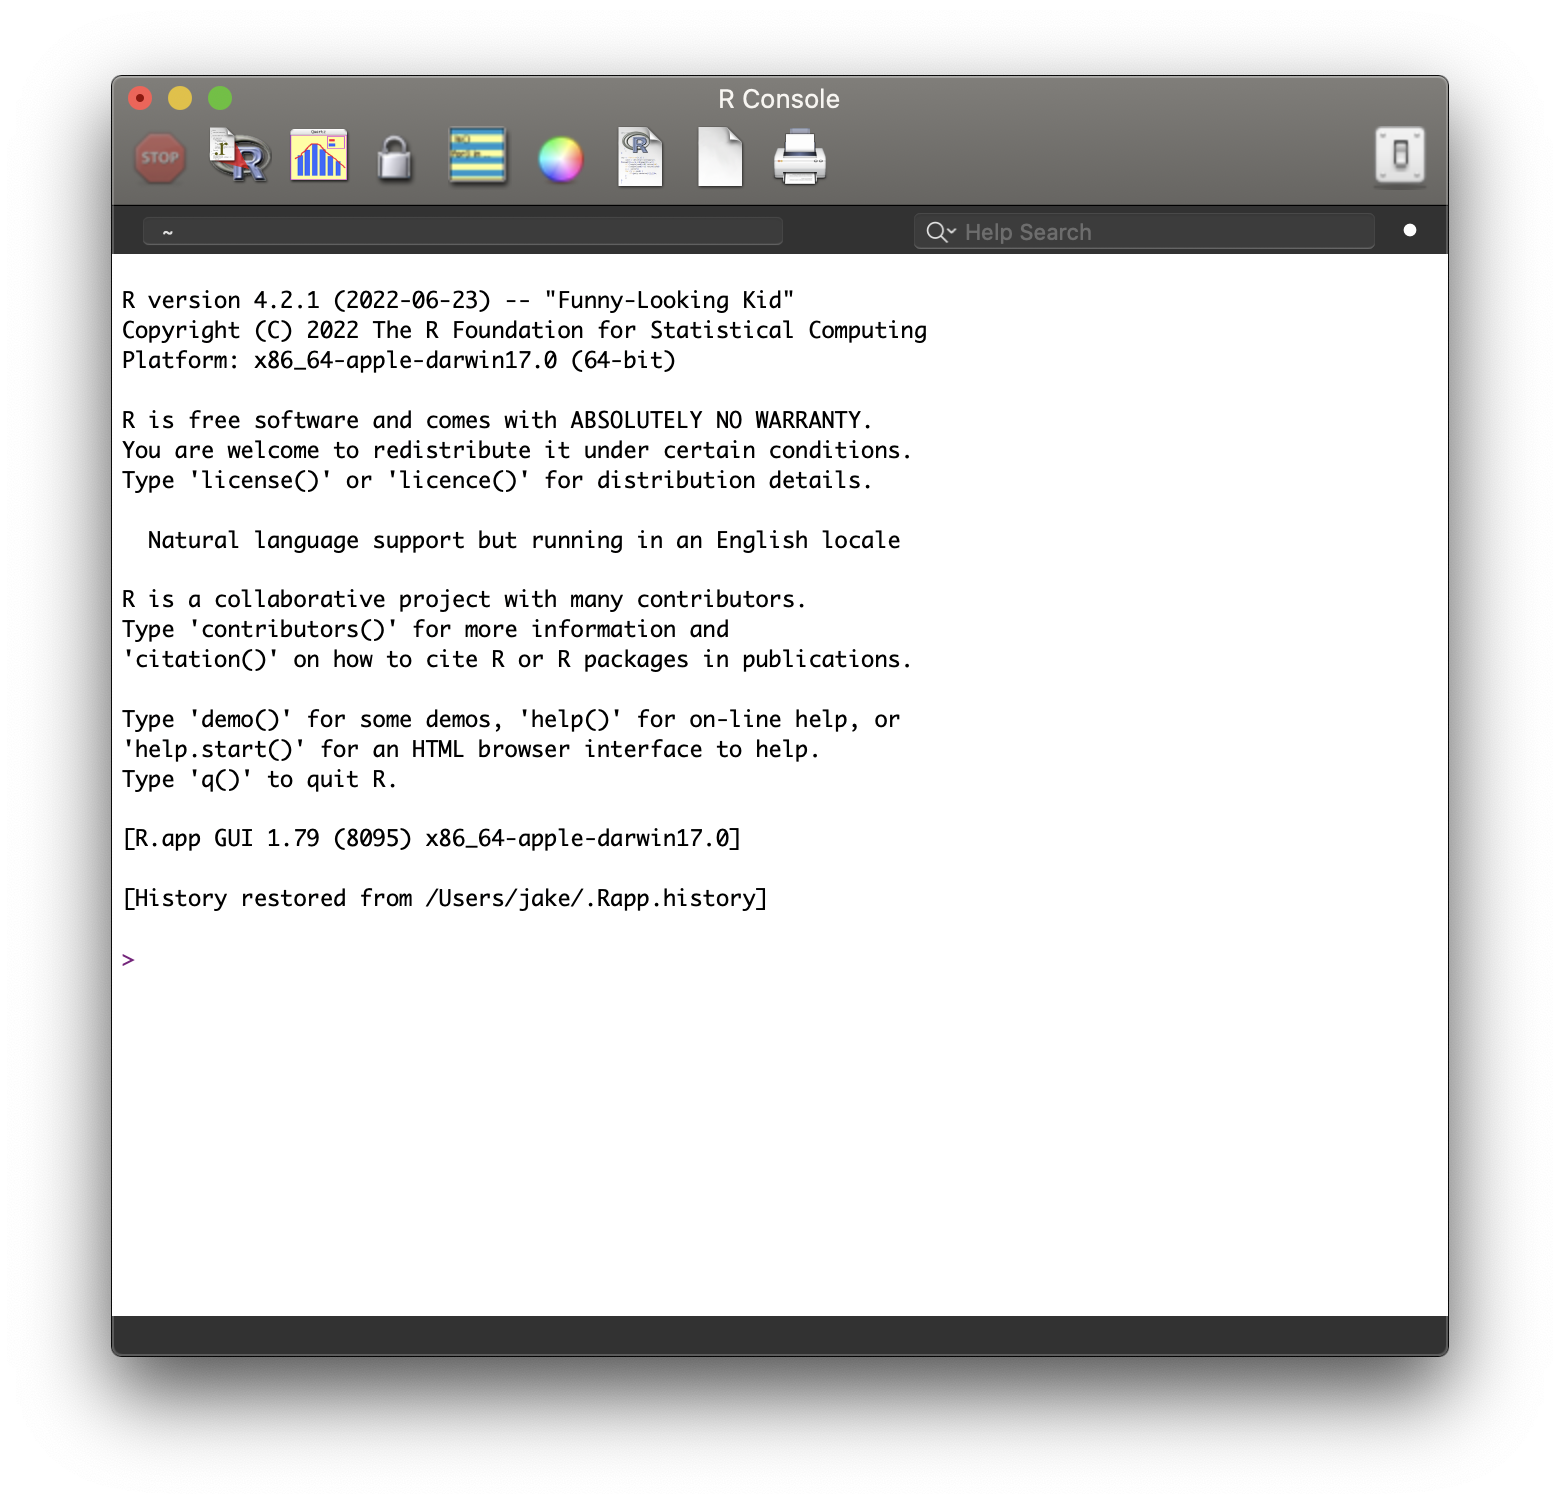
\includegraphics{img/R-app-interface.png}
\caption{The \texttt{R} graphical console}
\end{figure}

You can also work with \texttt{R} from a shell interface, but I will not be discussing this approach in this workshop.

\hypertarget{great-why-are-we-using-rstudio-then}{%
\subsection{Great, why are we using RStudio then?}\label{great-why-are-we-using-rstudio-then}}

RStudio is an ``\textbf{I}nteractive \textbf{D}evelopment \textbf{E}nvironment'' (IDE) for working with \texttt{R}. Without going into a lot of detail, that means that \texttt{R} lives on its own on your computer in a separate directory, and RStudio provides a bunch of better functionality for things like writing multiple files at once, making editing easier, autofilling code, and displaying plots. You can learn more about \href{https://www.rstudio.com/products/rstudio/}{RStudio here}.

With that out of the way, I am going to be sloppy in terminology and say/type ``\texttt{R}'' a lot of the times I mean ``RStudio''. I will be very clear if the distinction actually matters. RStudio is going to make your life way easier, and when you try to learn Python you are going to be sad :(

\hypertarget{the-parts-of-rstudio}{%
\section{The parts of RStudio}\label{the-parts-of-rstudio}}

The default layout of RStudio looks something like this (font sizes may vary):

\begin{figure}
\centering
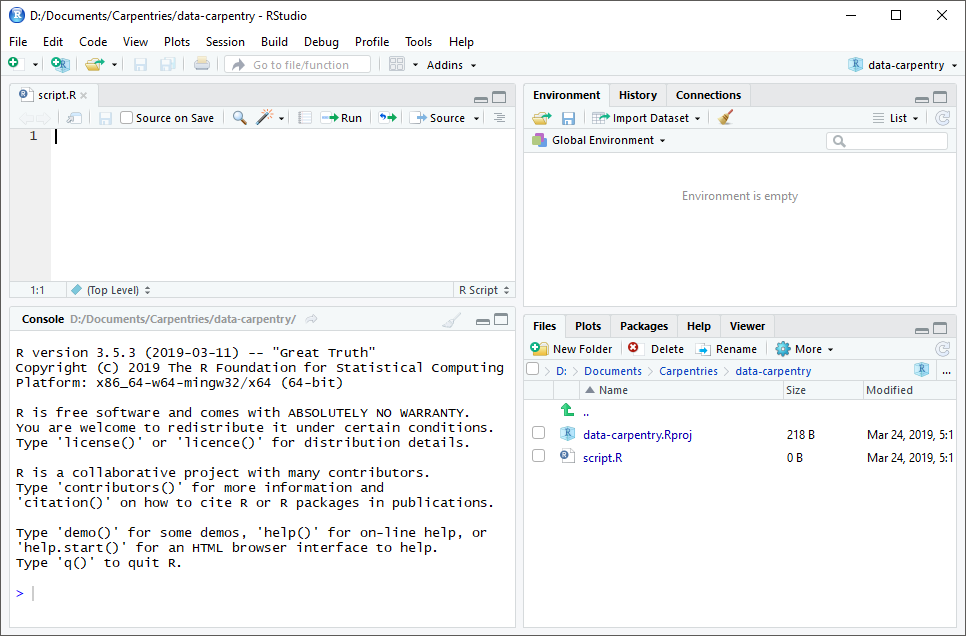
\includegraphics{img/R_00_Rstudio_01.png}
\caption{RStudio default layout, courtesy of \href{https://datacarpentry.org/r-socialsci/00-intro/index.html}{Data Carpentry}}
\end{figure}

RStudio always has 4 ``panes'' with various functions, which are in tabs (just like a web browser). The key ones for right now to pay attention are:

\begin{enumerate}
\def\labelenumi{\arabic{enumi}.}
\tightlist
\item
  The \texttt{Console} tab is the portal to interact directly with \texttt{R}. The \texttt{\textgreater{}} ``prompt'' is where you can type and execute commands (by hitting return). You can try this out right now by using it like a calculator - try \texttt{1\ +\ 1} if you like!
\item
  The \texttt{Files} tab shows the files in your \textbf{working directory}: like in the Windows Explorer or macOS Finder, files are displayed within folders. You can click on files to open them.
\item
  The \texttt{Help} tab shows documentation for \texttt{R} functions and packages--it is useful for learning how to use specific functions.
\item
  The \texttt{Plots} tab shows graphical output, and this is where the data visualizations we'll learn to make will (generally) appear.
\item
  The \texttt{Environment} tab shows the objects that exist in memory in your current \texttt{R} session. Without going into details, this is ``what you've done'' so far: data tables and variables you've created, etc.
\item
  Finally, the \texttt{Scripts} \textbf{pane} shows \emph{individual} tabs for each script and other RStudio file. Scripts (and other, more exotic file types like RMarkdown/.Rmd files) are documents that contain multiple \texttt{R} commands, like you'd type into the \texttt{Console}. However, unlike commands in the \texttt{Console}, these commands don't disappear as soon as they're run, and we can string them together to make workflows or even programs. This is where the real power of \texttt{R} will come from.
\end{enumerate}

You can change the layout of your Panes (and many other options) by going to the RStudio menu: \texttt{Tools\ \textgreater{}\ Global\ Options} and select \texttt{Pane\ Layout}.

You'll notice that my layout for RStudio looks quite different from the default, but you can always orient yourself by seeing what tab or pane I am in--these are always the same. I prefer giving myself more space for writing \texttt{R} scripts and markdown files, so I have given that specific Pane more space while minimizing the \texttt{History} pane.

While we're in Global Options, please make the following selections:

\begin{enumerate}
\def\labelenumi{\arabic{enumi}.}
\tightlist
\item
  Under \texttt{General}, uncheck all the boxes to do with restoring projects and workspaces. We want to make sure our code runs the same time every time (i.e., that our methods are reproducible), and letting RStudio load these will make this impossible:
\end{enumerate}

\begin{figure}
\centering
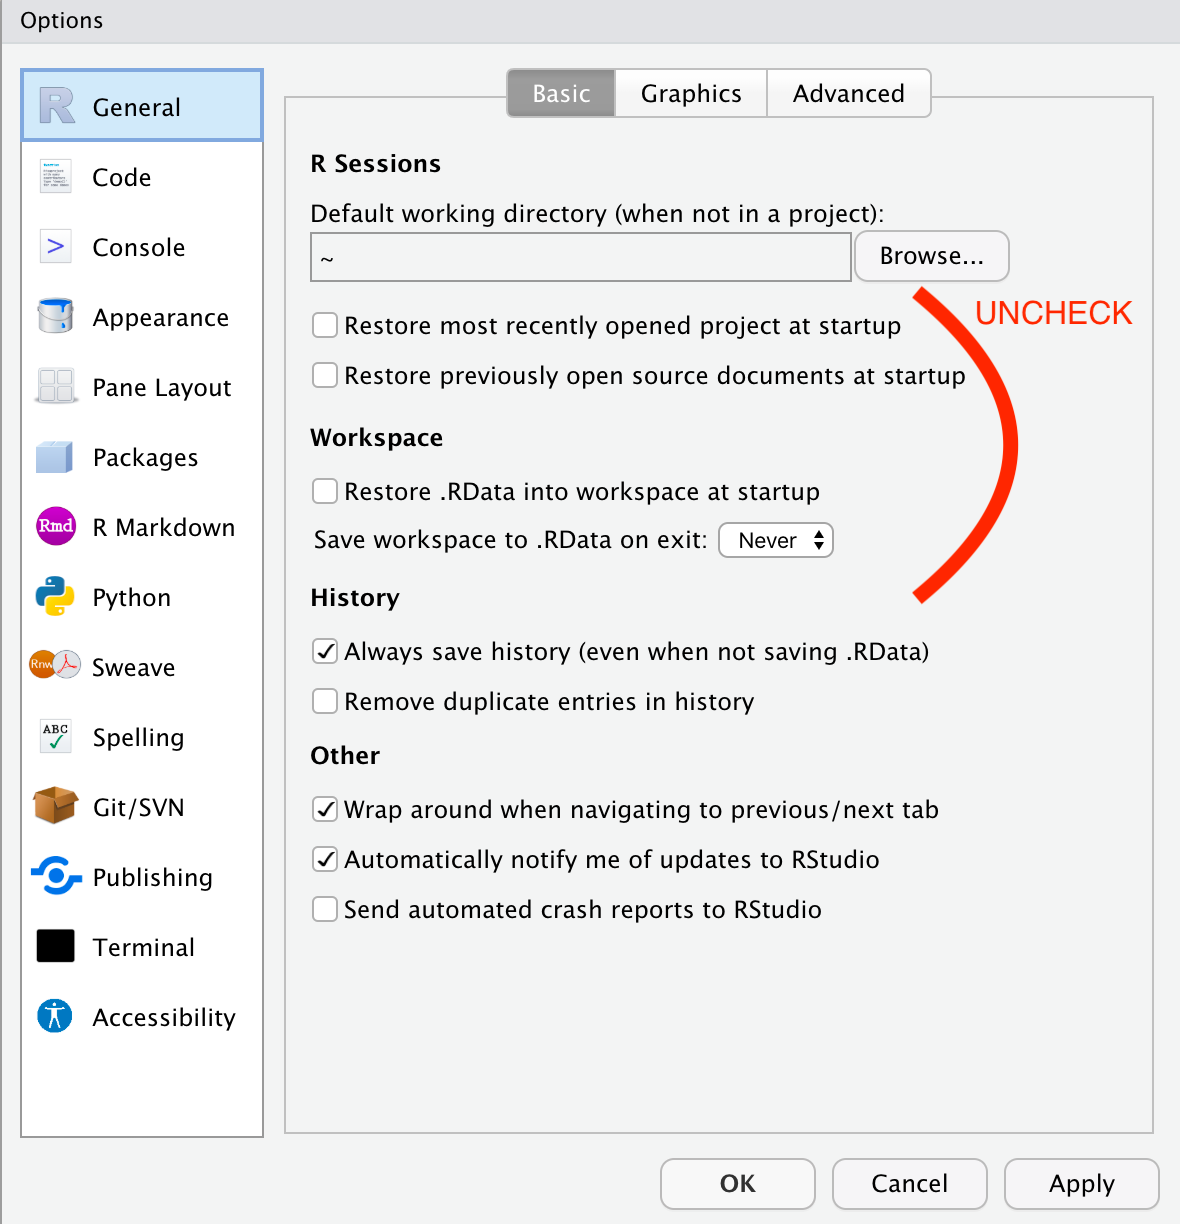
\includegraphics[width=4.16667in,height=\textheight]{img/global-options-settings.png}
\caption{Uncheck the options to restore various data and projects at startup.}
\end{figure}

\begin{enumerate}
\def\labelenumi{\arabic{enumi}.}
\setcounter{enumi}{1}
\tightlist
\item
  Make your life easier by setting up \textbf{autocompletion} for your code. Under the \texttt{Code\ \textgreater{}\ Completion} options, select the checkboxes to allow using \texttt{tab} for autocompletions, and also allowing multiline autocompletions. This means that RStudio will suggest functions and data for you if you hit \texttt{tab}, which will make you have to do way less typing:
\end{enumerate}

\begin{figure}
\centering
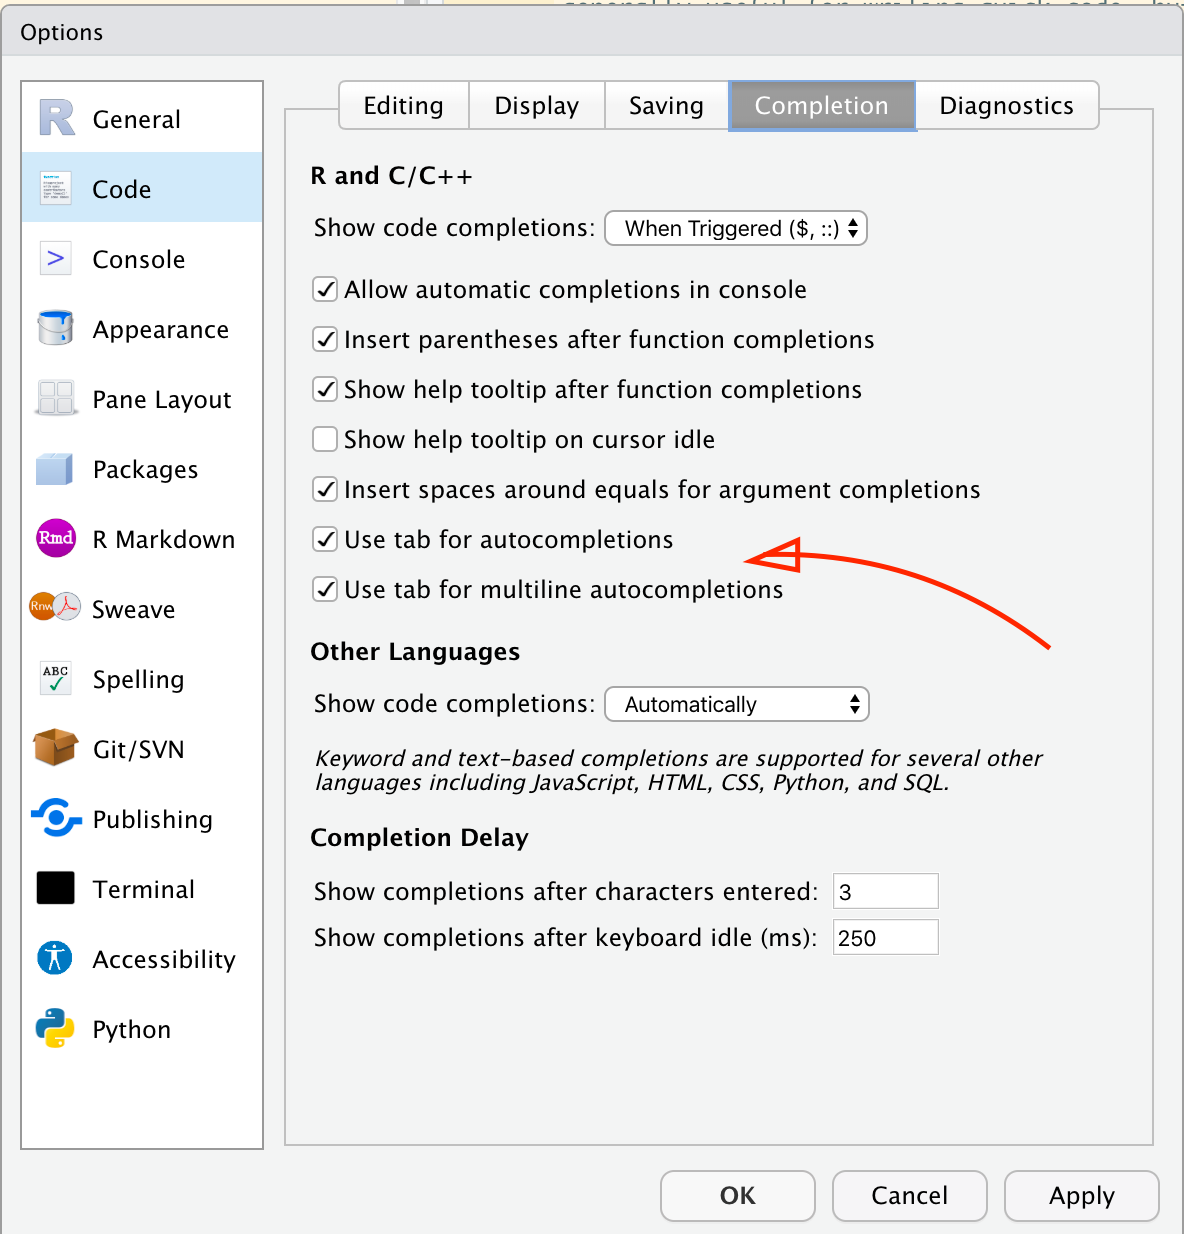
\includegraphics[width=4.16667in,height=\textheight]{img/code-autocompletion.png}
\caption{Check the boxes for tab and multiline autocompletions.}
\end{figure}

\hypertarget{the-working-directory-and-why-you-should-care}{%
\subsection{The ``working directory'' and why you should care}\label{the-working-directory-and-why-you-should-care}}

Before we move on to using \texttt{R} for real, we have one key general computing concept to tackle: the ``working directory''. The working directory is the folder on your computer in which \texttt{R} will look for files and save files.

When you need to tell \texttt{R} to \textbf{read in data from a file or output a file}, you will have to do so \textbf{in relation to your working directory}. Therefore, it is important that you know how to find your working directory and change it.

The easiest (but not best) way to do this is to use the \texttt{Files} pane. If you hit the ``gear'' icon in the \texttt{Files} pane menu, you'll see two commands to do with the working directory. You can \texttt{Go\ To\ Working\ Directory} to show you whatever \texttt{R} currently has set as the working directory. You can then navigate to any directory you want on your hard drive, and use the \texttt{Set\ As\ Working\ Directory} command to make that the working directory.

A better way to do this is to use the R commands \texttt{getwd()} and \texttt{setwd()}.

\begin{Shaded}
\begin{Highlighting}[]
\FunctionTok{getwd}\NormalTok{() }\CommentTok{\# will print the current working directory}
\end{Highlighting}
\end{Shaded}

\begin{verbatim}
## [1] "C:/Users/lhamilton/Documents/sensometrics-r-tutorial-2024"
\end{verbatim}

And we can manually change the working directory by using

\begin{Shaded}
\begin{Highlighting}[]
\FunctionTok{setwd}\NormalTok{(}\StringTok{"Enter/Your/Desired/Directory/Here"}\NormalTok{)}
\end{Highlighting}
\end{Shaded}

Notice that I am not running the second command, because it would cause an error!

When we use \texttt{R} to navigate directories, I recommend \textbf{always} using the forward slash: \texttt{/}, even though on Windows systems the typical slash is the backslash: \texttt{\textbackslash{}}. \texttt{R} will properly interpret the \texttt{/} for you in the context of your operating system, and this is more consistent with most modern code environments.

\hypertarget{extending-r-with-packages}{%
\section{\texorpdfstring{Extending \texttt{R} with packages}{Extending R with packages}}\label{extending-r-with-packages}}

One of the key advantages of \texttt{R} is that its open-source nature means that you can extend it to do all sorts of things. For example, for much of this workshop we are going to use the \texttt{tidyverse} packages and the \texttt{ca} package. There are various ways to install new packages, but the easiest way is to use the \texttt{Packages} tab. This will show you all the packages you currently have installed as an alphabetical list.

We install new packages using the \texttt{install.packages()} command. As part of the pre-work for the tutorial, you will have run the following commmands:

\begin{Shaded}
\begin{Highlighting}[]
\CommentTok{\# Install the tidyverse packages}
\FunctionTok{install.packages}\NormalTok{(}\StringTok{"tidyverse"}\NormalTok{)}
\CommentTok{\# Install the ca package}
\FunctionTok{install.packages}\NormalTok{(}\StringTok{"ca"}\NormalTok{)}
\end{Highlighting}
\end{Shaded}

While these commands will download packages and install them in a directory on your hard drive where \texttt{R} can find them, they \textbf{will not} make them immediately usable in an \texttt{R} programming session.

\hypertarget{loading-packages}{%
\subsection{Loading packages}\label{loading-packages}}

To actually use a package, you need to load it using the \texttt{library(\textless{}name\ of\ package\textgreater{})} command. So, for example, to load the \texttt{tidyverse} package we will use the command

\begin{Shaded}
\begin{Highlighting}[]
\FunctionTok{library}\NormalTok{(tidyverse)}
\end{Highlighting}
\end{Shaded}

\begin{verbatim}
## -- Attaching core tidyverse packages ------------------------ tidyverse 2.0.0 --
## v dplyr     1.1.4     v readr     2.1.4
## v forcats   1.0.0     v stringr   1.5.1
## v ggplot2   3.4.2     v tibble    3.2.1
## v lubridate 1.9.2     v tidyr     1.3.1
## v purrr     1.0.1     
## -- Conflicts ------------------------------------------ tidyverse_conflicts() --
## x dplyr::filter() masks stats::filter()
## x dplyr::lag()    masks stats::lag()
## i Use the conflicted package (<http://conflicted.r-lib.org/>) to force all conflicts to become errors
\end{verbatim}

You need to use multiple \texttt{library()} commands to load multiple packages, e.g.,

\begin{Shaded}
\begin{Highlighting}[]
\FunctionTok{library}\NormalTok{(tidyverse)}
\FunctionTok{library}\NormalTok{(ca)}
\end{Highlighting}
\end{Shaded}

If you want to know what packages you have loaded, you can run the \texttt{sessionInfo()} function, which will tell you a bunch of stuff, including the ``attached'' packages:

\begin{Shaded}
\begin{Highlighting}[]
\FunctionTok{sessionInfo}\NormalTok{()}
\end{Highlighting}
\end{Shaded}

\begin{verbatim}
## R version 4.3.1 (2023-06-16 ucrt)
## Platform: x86_64-w64-mingw32/x64 (64-bit)
## Running under: Windows 10 x64 (build 19045)
## 
## Matrix products: default
## 
## 
## locale:
## [1] LC_COLLATE=English_United States.utf8 
## [2] LC_CTYPE=English_United States.utf8   
## [3] LC_MONETARY=English_United States.utf8
## [4] LC_NUMERIC=C                          
## [5] LC_TIME=English_United States.utf8    
## 
## time zone: America/New_York
## tzcode source: internal
## 
## attached base packages:
## [1] stats     graphics  grDevices utils     datasets  methods   base     
## 
## other attached packages:
##  [1] ca_0.71.1       lubridate_1.9.2 forcats_1.0.0   stringr_1.5.1  
##  [5] dplyr_1.1.4     purrr_1.0.1     readr_2.1.4     tidyr_1.3.1    
##  [9] tibble_3.2.1    ggplot2_3.4.2   tidyverse_2.0.0
## 
## loaded via a namespace (and not attached):
##  [1] gtable_0.3.3      compiler_4.3.1    tidyselect_1.2.1  scales_1.3.0     
##  [5] yaml_2.3.7        fastmap_1.1.1     R6_2.5.1          generics_0.1.3   
##  [9] knitr_1.43        bookdown_0.34     munsell_0.5.1     pillar_1.9.0     
## [13] tzdb_0.4.0        rlang_1.1.1       utf8_1.2.4        stringi_1.7.12   
## [17] xfun_0.39         timechange_0.2.0  cli_3.6.1         withr_3.0.0      
## [21] magrittr_2.0.3    digest_0.6.33     grid_4.3.1        rstudioapi_0.15.0
## [25] hms_1.1.3         lifecycle_1.0.4   vctrs_0.6.5       evaluate_0.23    
## [29] glue_1.6.2        fansi_1.0.6       colorspace_2.1-0  rmarkdown_2.23   
## [33] tools_4.3.1       pkgconfig_2.0.3   htmltools_0.5.8.1
\end{verbatim}

Finally, you can also load (and unload) packages using the \texttt{Packages} tab, by clicking the checkbox next to the name of the package you want to load (or unload).

Typically, we think it's a good idea to put all of your \texttt{library()} function calls at the top of your script, so that you don't try to call a function from a package that has been loaded ``later'' (further down) in your script and cause an error.

\hypertarget{making-r-do-stuff}{%
\section{\texorpdfstring{Making \texttt{R} do stuff}{Making R do stuff}}\label{making-r-do-stuff}}

We can make \texttt{R} act as a basic calculator:

\begin{Shaded}
\begin{Highlighting}[]
\DecValTok{2} \SpecialCharTok{+} \DecValTok{3}
\end{Highlighting}
\end{Shaded}

\begin{verbatim}
## [1] 5
\end{verbatim}

\begin{Shaded}
\begin{Highlighting}[]
\DecValTok{4} \SpecialCharTok{/} \DecValTok{124}
\end{Highlighting}
\end{Shaded}

\begin{verbatim}
## [1] 0.03225806
\end{verbatim}

Mostly, we will be using \texttt{R} for writing complex, functional programs, in which we \textbf{assign variables} and use those variables in \textbf{functions}:

\begin{Shaded}
\begin{Highlighting}[]
\NormalTok{x }\OtherTok{\textless{}{-}} \StringTok{"dog"}
\FunctionTok{ifelse}\NormalTok{(x }\SpecialCharTok{==} \StringTok{"cat"}\NormalTok{, }\StringTok{"Definitely feline!"}\NormalTok{, }\StringTok{"You\textquotesingle{}ve got something else there!"}\NormalTok{)}
\end{Highlighting}
\end{Shaded}

\begin{verbatim}
## [1] "You've got something else there!"
\end{verbatim}

\hypertarget{livecoding-along}{%
\section{Livecoding along}\label{livecoding-along}}

We've now covered the \texttt{Console} tab and the \texttt{Scripts} pane. These are both areas in which you can write and execute code, but they work a little differently. The \texttt{Console} is the place to run code that is short and easy to type, or that you're experimenting with. It will allow you to write a single line of code, and after you hit \texttt{return}, \texttt{R} will execute the command. This is great for ``interactive programming'', but it isn't so great for building up a complex workflow, or for following along with this workshop!

This is why I have recommended that you create a new script to follow along with this workshop. You get a new script by going to \texttt{File\ \textgreater{}\ New\ File\ \textgreater{}\ R\ Script}. You can write multiple lines of code and then execute each one in any order (although keeping a logical sequence from top to bottom will help you keep track of what you're doing). In an \texttt{R} script, everything is expected to be valid R code.

\begin{Shaded}
\begin{Highlighting}[]
\NormalTok{You can}\StringTok{\textquotesingle{}t write this in an R script because it is plain text.  This will}
\StringTok{cause an error.}

\StringTok{\# If you want to write text or notes to yourself, use the "\#" symbol at the start of }
\StringTok{\# every line to "comment" out that line.  You can also put "\#" in the middle of}
\StringTok{\# a line in order to add a comment {-} everything after will be ignored.}

\StringTok{1 + 1 \# this is valid R syntax}

\StringTok{print("hello world") \# this is also valid R syntax}
\end{Highlighting}
\end{Shaded}

To run code from your \texttt{R} script, put your cursor on the line you want to run and either hit the run button with the green arrow at the top left or (my preferred method) type \texttt{cmd\ +\ return} (on Mac) or \texttt{ctrl\ +\ return} (on PC).

\hypertarget{summary-and-next-steps}{%
\section{Summary and next steps}\label{summary-and-next-steps}}

We've now run through briefly the ``what'' of the \texttt{R}/RStudio interface. Next, we're going to dive into importing some sensory datasets and processing them for visualization.

\hypertarget{importing-and-wrangling-data}{%
\chapter{Importing and wrangling data}\label{importing-and-wrangling-data}}

Now that everyone is on the same page for how we're going to use \texttt{R}, we're going to dive right into importing our data into \texttt{R}, exploring it, and--most importantly--visualizing it. In this part of the tutorial, we are going to focus on getting data into \texttt{R} and manipulating it.

Personally, I prefer to see the reason for doing something, rather than being shown a bunch of building blocks and not seeing how they fit together. Therefore, we're going to start off this section with a complete work flow for importing and visualizing some real results, and then work backward as we unpack how and why we've taken particular steps.

\hypertarget{motivation-exploring-berry-and-cider-cataliking-data}{%
\section{Motivation: exploring berry and cider CATA/liking data}\label{motivation-exploring-berry-and-cider-cataliking-data}}

Before we begin, we need to make sure we've loaded the packages we're going to use.

\begin{Shaded}
\begin{Highlighting}[]
\CommentTok{\# This package is actually a set of utility packages we will use a lot}
\FunctionTok{library}\NormalTok{(tidyverse)}
\end{Highlighting}
\end{Shaded}

The plan here is to present ``full'' workflows for data import, wrangling, and visualization below so as to give a skeleton to work through. This is going to look like a lot of code at once, but I don't use anything in these workflows that we will not be covering (in some way!) today. Hopefully, by the end of today's workshop you will be able both to understand and dissect complex code and use it to build your own analyses and visualizations.

\hypertarget{berries}{%
\subsection{Berries}\label{berries}}

Here we are going to import and process data from a study on berries. These data come from a large, central-location study on berries, the methodological details of which are published in Yeung et al. (2021). Very briefly, the data describe the attributes and liking scores reported by consumers for a variety of berries across multiple CLTs. A total of 969 participants (\texttt{Subject\ Code}) and 23 berries (\texttt{Sample\ Name}) were involved in these tests, with only one species of berry (blackberry, blueberry, raspberry, or strawberry) presented during each CLT. In the actual experimental design, subjects got multiple sample sets (so there are \emph{not} 969 unique subjects), but here we will treat them as unique for ease of description.

\begin{Shaded}
\begin{Highlighting}[]
\CommentTok{\# Import the data}
\NormalTok{raw\_berry\_data }\OtherTok{\textless{}{-}} 
  \FunctionTok{read\_csv}\NormalTok{(}\AttributeTok{file =} \StringTok{"data/clt{-}berry{-}data.csv"}\NormalTok{) }\SpecialCharTok{\%\textgreater{}\%}
  \FunctionTok{select}\NormalTok{(}\FunctionTok{where}\NormalTok{(}\SpecialCharTok{\textasciitilde{}} \SpecialCharTok{!}\FunctionTok{all}\NormalTok{(}\FunctionTok{is.na}\NormalTok{(.)))) }

\NormalTok{cleaned\_berry\_data }\OtherTok{\textless{}{-}}
\NormalTok{  raw\_berry\_data }\SpecialCharTok{\%\textgreater{}\%}
  \CommentTok{\# Get the relevant columns}
  \FunctionTok{select}\NormalTok{(}\StringTok{\textasciigrave{}}\AttributeTok{Subject Code}\StringTok{\textasciigrave{}}\NormalTok{, }
\NormalTok{         berry,}
\NormalTok{         sample,}
         \FunctionTok{starts\_with}\NormalTok{(}\StringTok{"cata\_"}\NormalTok{), }
         \FunctionTok{contains}\NormalTok{(}\StringTok{"overall"}\NormalTok{)) }\SpecialCharTok{\%\textgreater{}\%}
  \CommentTok{\# Rescale the LAM and US scales to a 9{-}pt range}
  \FunctionTok{mutate}\NormalTok{(}\AttributeTok{lms\_overall =}\NormalTok{ (lms\_overall }\SpecialCharTok{+} \DecValTok{100}\NormalTok{) }\SpecialCharTok{*}\NormalTok{ (}\DecValTok{8} \SpecialCharTok{/} \DecValTok{200}\NormalTok{) }\SpecialCharTok{+} \DecValTok{1}\NormalTok{,}
         \AttributeTok{us\_overall =}\NormalTok{ (us\_overall }\SpecialCharTok{+} \DecValTok{0}\NormalTok{) }\SpecialCharTok{*}\NormalTok{ (}\DecValTok{8} \SpecialCharTok{/} \DecValTok{15}\NormalTok{) }\SpecialCharTok{+} \DecValTok{1}\NormalTok{) }\SpecialCharTok{\%\textgreater{}\%}
  \CommentTok{\# Switch the 3 overall liking columns into a single column}
  \FunctionTok{pivot\_longer}\NormalTok{(}\FunctionTok{contains}\NormalTok{(}\StringTok{"overall"}\NormalTok{),}
               \AttributeTok{names\_to =} \StringTok{"hedonic\_scale"}\NormalTok{,}
               \AttributeTok{values\_to =} \StringTok{"rating"}\NormalTok{,}
               \AttributeTok{values\_drop\_na =} \ConstantTok{TRUE}\NormalTok{) }\SpecialCharTok{\%\textgreater{}\%}
  \CommentTok{\# Let\textquotesingle{}s make all the CATA variables into a single column to make life easier}
  \CommentTok{\# (and get rid of those NAs)}
  \FunctionTok{pivot\_longer}\NormalTok{(}\FunctionTok{starts\_with}\NormalTok{(}\StringTok{"cata\_"}\NormalTok{),}
               \AttributeTok{names\_to =} \StringTok{"cata\_variable"}\NormalTok{,}
               \AttributeTok{values\_to =} \StringTok{"checked"}\NormalTok{,}
               \AttributeTok{names\_transform =} \SpecialCharTok{\textasciitilde{}}\FunctionTok{str\_remove}\NormalTok{(., }\StringTok{"cata\_"}\NormalTok{),}
               \AttributeTok{values\_drop\_na =} \ConstantTok{TRUE}\NormalTok{)}

\NormalTok{berry\_penalty\_analysis\_data }\OtherTok{\textless{}{-}} 
\NormalTok{  cleaned\_berry\_data }\SpecialCharTok{\%\textgreater{}\%}
  \FunctionTok{group\_by}\NormalTok{(berry, cata\_variable, checked) }\SpecialCharTok{\%\textgreater{}\%}
  \FunctionTok{summarize}\NormalTok{(}\AttributeTok{penalty\_lift =} \FunctionTok{mean}\NormalTok{(rating),}
            \AttributeTok{count =} \FunctionTok{n}\NormalTok{()) }\SpecialCharTok{\%\textgreater{}\%}
  \FunctionTok{ungroup}\NormalTok{() }

\CommentTok{\# Make a plot of the overall penalty/lift for checked attributes}
\NormalTok{p1\_berry\_penalty }\OtherTok{\textless{}{-}} 
\NormalTok{  berry\_penalty\_analysis\_data }\SpecialCharTok{\%\textgreater{}\%}
  \FunctionTok{select}\NormalTok{(}\SpecialCharTok{{-}}\NormalTok{count) }\SpecialCharTok{\%\textgreater{}\%}
  \FunctionTok{pivot\_wider}\NormalTok{(}\AttributeTok{names\_from =}\NormalTok{ checked,}
              \AttributeTok{values\_from =}\NormalTok{ penalty\_lift,}
              \AttributeTok{names\_prefix =} \StringTok{"checked\_"}\NormalTok{) }\SpecialCharTok{\%\textgreater{}\%}
  \FunctionTok{group\_by}\NormalTok{(berry, cata\_variable) }\SpecialCharTok{\%\textgreater{}\%}
  \FunctionTok{summarize}\NormalTok{(}\AttributeTok{penalty\_lift =}\NormalTok{ checked\_1 }\SpecialCharTok{{-}}\NormalTok{ checked\_0) }\SpecialCharTok{\%\textgreater{}\%}
  \CommentTok{\# We can tidy up our CATA labels}
  \FunctionTok{separate}\NormalTok{(cata\_variable, }
           \AttributeTok{into =} \FunctionTok{c}\NormalTok{(}\StringTok{"mode"}\NormalTok{, }\StringTok{"variable"}\NormalTok{), }
           \AttributeTok{sep =} \StringTok{"\_"}\NormalTok{) }\SpecialCharTok{\%\textgreater{}\%}
  \CommentTok{\# Fix a typo}
  \FunctionTok{mutate}\NormalTok{(}\AttributeTok{mode =} \FunctionTok{str\_replace}\NormalTok{(mode, }\StringTok{"appearane"}\NormalTok{, }\StringTok{"appearance"}\NormalTok{)) }\SpecialCharTok{\%\textgreater{}\%}
  \FunctionTok{mutate}\NormalTok{(}\AttributeTok{mode =} \FunctionTok{case\_when}\NormalTok{(mode }\SpecialCharTok{==} \StringTok{"taste"} \SpecialCharTok{\textasciitilde{}} \StringTok{"(T)"}\NormalTok{,}
\NormalTok{                          mode }\SpecialCharTok{==} \StringTok{"appearance"} \SpecialCharTok{\textasciitilde{}} \StringTok{"(A)"}\NormalTok{)) }\SpecialCharTok{\%\textgreater{}\%}
  \FunctionTok{unite}\NormalTok{(variable, mode, }\AttributeTok{col =} \StringTok{"cata\_variable"}\NormalTok{, }\AttributeTok{sep =} \StringTok{" "}\NormalTok{) }\SpecialCharTok{\%\textgreater{}\%}
  \CommentTok{\# We are using a function from tidytext that makes faceting the final figure}
  \CommentTok{\# easier}
  \FunctionTok{mutate}\NormalTok{(}\AttributeTok{cata\_variable =}\NormalTok{ tidytext}\SpecialCharTok{::}\FunctionTok{reorder\_within}\NormalTok{(}\AttributeTok{x =}\NormalTok{ cata\_variable,}
                                                  \AttributeTok{by =}\NormalTok{ penalty\_lift,}
                                                  \AttributeTok{within =}\NormalTok{ berry)) }\SpecialCharTok{\%\textgreater{}\%}
  \CommentTok{\#And finally we plot!}
  \FunctionTok{ggplot}\NormalTok{(}\AttributeTok{mapping =} \FunctionTok{aes}\NormalTok{(}\AttributeTok{x =}\NormalTok{ cata\_variable, }\AttributeTok{y =}\NormalTok{ penalty\_lift)) }\SpecialCharTok{+}
  \FunctionTok{geom\_col}\NormalTok{(}\FunctionTok{aes}\NormalTok{(}\AttributeTok{fill =}\NormalTok{ penalty\_lift), }\AttributeTok{color =} \StringTok{"white"}\NormalTok{, }\AttributeTok{show.legend =} \ConstantTok{FALSE}\NormalTok{) }\SpecialCharTok{+} 
  \FunctionTok{facet\_wrap}\NormalTok{(}\SpecialCharTok{\textasciitilde{}}\NormalTok{berry, }\AttributeTok{scales =} \StringTok{"free"}\NormalTok{, }\AttributeTok{nrow =} \DecValTok{1}\NormalTok{) }\SpecialCharTok{+} 
\NormalTok{  tidytext}\SpecialCharTok{::}\FunctionTok{scale\_x\_reordered}\NormalTok{() }\SpecialCharTok{+} 
  \FunctionTok{coord\_flip}\NormalTok{() }\SpecialCharTok{+} 
  \FunctionTok{theme\_classic}\NormalTok{() }\SpecialCharTok{+} 
  \FunctionTok{scale\_fill\_gradient}\NormalTok{(}\AttributeTok{low =} \StringTok{"tan"}\NormalTok{, }\AttributeTok{high =} \StringTok{"darkgreen"}\NormalTok{) }\SpecialCharTok{+} 
  \FunctionTok{labs}\NormalTok{(}\AttributeTok{x =} \ConstantTok{NULL}\NormalTok{, }\AttributeTok{y =} \ConstantTok{NULL}\NormalTok{,}
       \AttributeTok{title =} \StringTok{"Penalty / Lift Analysis"}\NormalTok{,}
       \AttributeTok{subtitle =} \StringTok{"displays the mean difference (within berries) for when a CATA variable is checked}\SpecialCharTok{\textbackslash{}n}\StringTok{or un{-}checked"}\NormalTok{)}

\NormalTok{p1\_berry\_penalty}
\end{Highlighting}
\end{Shaded}

\begin{center}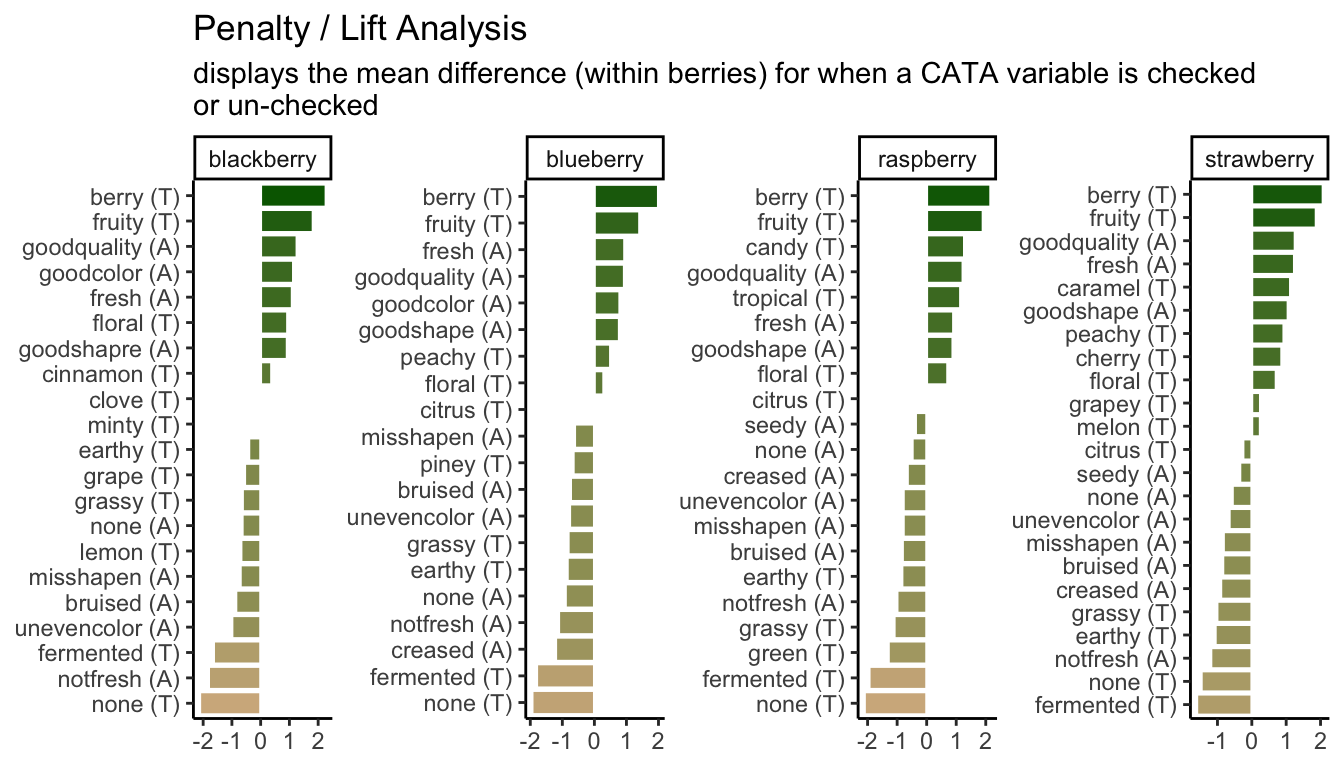
\includegraphics{02-import-wrangle-export_files/figure-latex/berry-full-penalty-1} \end{center}

\hypertarget{cider}{%
\subsection{Cider}\label{cider}}

Now, let's get our cider data. These data come from a small consumer study on 3 commercial ``hard'' (alcoholic) ciders, served in two conditions (chilled or unchilled) to 48 consumers, who used a pre-defined CATA lexicon, rated overall liking, and evaluated cider ``dryness'' on a 4-pt, structured line scale. The full details of the study are published in Calvert et al. (2022).

\begin{Shaded}
\begin{Highlighting}[]
\NormalTok{raw\_cider\_data }\OtherTok{\textless{}{-}} 
  \FunctionTok{read\_csv}\NormalTok{(}\StringTok{"data/CiderDryness\_SensoryDATA.csv"}\NormalTok{)}

\NormalTok{cider\_penalty\_data }\OtherTok{\textless{}{-}} 
\NormalTok{  raw\_cider\_data }\SpecialCharTok{\%\textgreater{}\%}
  \FunctionTok{pivot\_longer}\NormalTok{(Fresh\_Apples}\SpecialCharTok{:}\NormalTok{Synthetic,}
               \AttributeTok{names\_to =} \StringTok{"cata\_variable"}\NormalTok{,}
               \AttributeTok{values\_to =} \StringTok{"checked"}\NormalTok{) }\SpecialCharTok{\%\textgreater{}\%}
  \FunctionTok{group\_by}\NormalTok{(cata\_variable, checked) }\SpecialCharTok{\%\textgreater{}\%}
  \FunctionTok{summarize}\NormalTok{(}\AttributeTok{rating =} \FunctionTok{mean}\NormalTok{(Liking),}
            \AttributeTok{count =} \FunctionTok{n}\NormalTok{()) }\SpecialCharTok{\%\textgreater{}\%}
  \FunctionTok{mutate}\NormalTok{(}\AttributeTok{proportion =}\NormalTok{ count }\SpecialCharTok{/} \FunctionTok{sum}\NormalTok{(count)) }\SpecialCharTok{\%\textgreater{}\%}
  \FunctionTok{ungroup}\NormalTok{()}

\CommentTok{\# Define the "important" penalty/lift zones}

\NormalTok{zones }\OtherTok{\textless{}{-}} 
  \FunctionTok{tribble}\NormalTok{(}\SpecialCharTok{\textasciitilde{}}\NormalTok{penalty\_lift, }\SpecialCharTok{\textasciitilde{}}\NormalTok{xmin, }\SpecialCharTok{\textasciitilde{}}\NormalTok{xmax, }\SpecialCharTok{\textasciitilde{}}\NormalTok{ymin, }\SpecialCharTok{\textasciitilde{}}\NormalTok{ymax,}
          \StringTok{"penalty"}\NormalTok{, }\FloatTok{0.25}\NormalTok{, }\ConstantTok{Inf}\NormalTok{, }\SpecialCharTok{{-}}\ConstantTok{Inf}\NormalTok{, }\SpecialCharTok{{-}}\DecValTok{1}\NormalTok{,}
          \StringTok{"lift"}\NormalTok{, }\FloatTok{0.25}\NormalTok{, }\ConstantTok{Inf}\NormalTok{, }\DecValTok{1}\NormalTok{, }\ConstantTok{Inf}\NormalTok{)}

\CommentTok{\# Let\textquotesingle{}s make a plot where we take into account the frequency of checking as well}
\CommentTok{\# as the penalty}
\NormalTok{p2\_cider\_penalty }\OtherTok{\textless{}{-}} 
\NormalTok{  cider\_penalty\_data }\SpecialCharTok{\%\textgreater{}\%}
  \FunctionTok{select}\NormalTok{(}\SpecialCharTok{{-}}\NormalTok{count, }\SpecialCharTok{{-}}\NormalTok{proportion) }\SpecialCharTok{\%\textgreater{}\%}
  \FunctionTok{pivot\_wider}\NormalTok{(}\AttributeTok{names\_from =}\NormalTok{ checked,}
              \AttributeTok{values\_from =}\NormalTok{ rating) }\SpecialCharTok{\%\textgreater{}\%}
  \FunctionTok{mutate}\NormalTok{(}\AttributeTok{penalty =} \StringTok{\textasciigrave{}}\AttributeTok{1}\StringTok{\textasciigrave{}} \SpecialCharTok{{-}} \StringTok{\textasciigrave{}}\AttributeTok{0}\StringTok{\textasciigrave{}}\NormalTok{) }\SpecialCharTok{\%\textgreater{}\%}
  \FunctionTok{left\_join}\NormalTok{(cider\_penalty\_data }\SpecialCharTok{\%\textgreater{}\%}
              \FunctionTok{filter}\NormalTok{(checked }\SpecialCharTok{==} \DecValTok{1}\NormalTok{) }\SpecialCharTok{\%\textgreater{}\%}
              \FunctionTok{select}\NormalTok{(cata\_variable, proportion)) }\SpecialCharTok{\%\textgreater{}\%}
  \CommentTok{\# And now we plot!}
  \FunctionTok{ggplot}\NormalTok{(}\FunctionTok{aes}\NormalTok{(}\AttributeTok{x =}\NormalTok{ proportion, }\AttributeTok{y =}\NormalTok{ penalty)) }\SpecialCharTok{+} 
  \FunctionTok{geom\_hline}\NormalTok{(}\AttributeTok{yintercept =} \DecValTok{0}\NormalTok{) }\SpecialCharTok{+} 
  \FunctionTok{geom\_rect}\NormalTok{(}\FunctionTok{aes}\NormalTok{(}\AttributeTok{xmin =}\NormalTok{ xmin, }\AttributeTok{ymin =}\NormalTok{ ymin, }
                \AttributeTok{xmax =}\NormalTok{ xmax, }\AttributeTok{ymax =}\NormalTok{ ymax,}
                \AttributeTok{fill =}\NormalTok{ penalty\_lift, }\AttributeTok{color =}\NormalTok{ penalty\_lift),}
            \AttributeTok{data =}\NormalTok{ zones, }
            \AttributeTok{inherit.aes =} \ConstantTok{FALSE}\NormalTok{,}
            \AttributeTok{linetype =} \DecValTok{2}\NormalTok{) }\SpecialCharTok{+} 
  \FunctionTok{geom\_point}\NormalTok{() }\SpecialCharTok{+} 
\NormalTok{  ggrepel}\SpecialCharTok{::}\FunctionTok{geom\_label\_repel}\NormalTok{(}\FunctionTok{aes}\NormalTok{(}\AttributeTok{label =}\NormalTok{ cata\_variable), }\AttributeTok{alpha =} \DecValTok{2}\SpecialCharTok{/}\DecValTok{3}\NormalTok{) }\SpecialCharTok{+} 
  \FunctionTok{scale\_fill\_manual}\NormalTok{(}\StringTok{"penalty / lift zone:"}\NormalTok{, }
                    \AttributeTok{values =} \FunctionTok{alpha}\NormalTok{(}\FunctionTok{c}\NormalTok{( }\StringTok{"darkgreen"}\NormalTok{, }\StringTok{"tan"}\NormalTok{), }\AttributeTok{alpha =} \DecValTok{1}\SpecialCharTok{/}\DecValTok{4}\NormalTok{)) }\SpecialCharTok{+} 
  \FunctionTok{scale\_color\_manual}\NormalTok{(}\ConstantTok{NULL}\NormalTok{, }\AttributeTok{values =} \FunctionTok{c}\NormalTok{( }\StringTok{"darkgreen"}\NormalTok{, }\StringTok{"tan"}\NormalTok{), }\AttributeTok{breaks =} \ConstantTok{NULL}\NormalTok{) }\SpecialCharTok{+} 
  \FunctionTok{theme\_bw}\NormalTok{() }\SpecialCharTok{+} 
  \FunctionTok{theme}\NormalTok{(}\AttributeTok{panel.grid.minor =} \FunctionTok{element\_blank}\NormalTok{(),}
        \AttributeTok{panel.grid.major =} \FunctionTok{element\_blank}\NormalTok{(),}
        \AttributeTok{legend.position =} \StringTok{"top"}\NormalTok{) }\SpecialCharTok{+} 
  \FunctionTok{labs}\NormalTok{(}\AttributeTok{x =} \StringTok{"Proportion of checks for CATA attribute"}\NormalTok{,}
       \AttributeTok{y =} \StringTok{"Change in average liking when CATA}\SpecialCharTok{\textbackslash{}n}\StringTok{attribute is checked"}\NormalTok{,}
       \AttributeTok{title =} \StringTok{"Penalty/Lift Analysis"}\NormalTok{,}
       \AttributeTok{subtitle =} \StringTok{"in which average change is plotted against check frequency"}\NormalTok{)}

\NormalTok{p2\_cider\_penalty}
\end{Highlighting}
\end{Shaded}

\begin{center}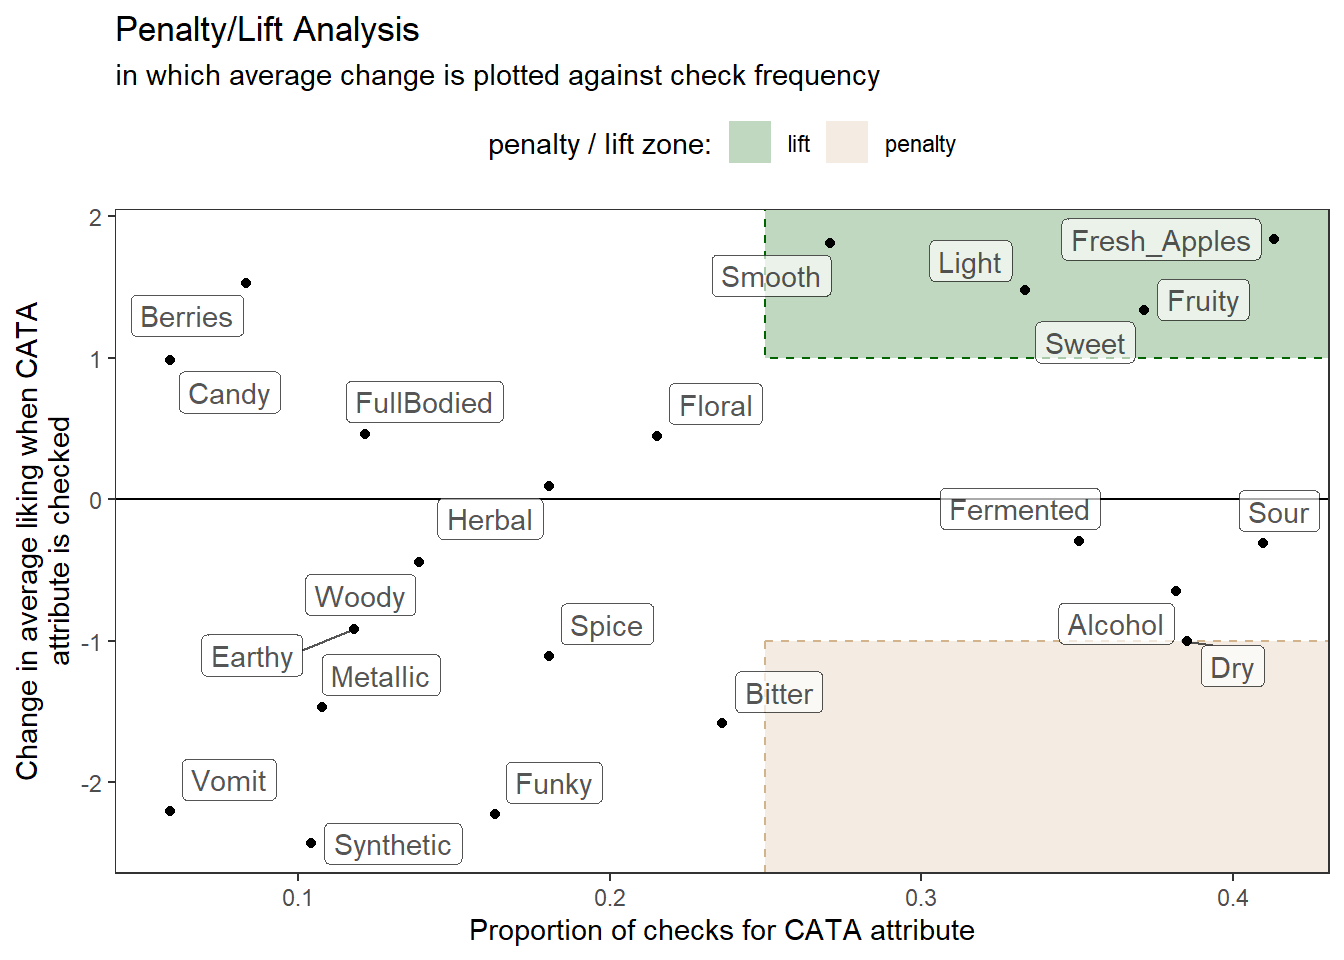
\includegraphics{02-import-wrangle-export_files/figure-latex/cider-full-penalty-1} \end{center}

\hypertarget{publication-quality}{%
\subsection{``Publication quality''}\label{publication-quality}}

What do we mean by ``publication quality'' visualizations? Neither of us are theorists of visualization--for that, we would recommend that you look at the excellent work from \href{https://clauswilke.com/dataviz/}{Claus Wilke} and \href{https://socviz.co/index.html\#preface}{Kieran Healey}. We will not be discussing (in any detail) ideas about which color palettes best communicate different types of data, what kinds of displays are most effective (box plots vs violin plots vs \ldots), or whether pie charts are really so bad (mostly yes).

Rather, we have noticed that most \texttt{R} packages for data analysis provide visualizations as part of their output, and many sensory scientists are using these \emph{default} outputs in publications. This is annoying because often these visualizations are meant to be part of the data exploration/analysis process: they are not polished or they don't display the data to its best advantage (whatever that is for the particular case). In this workshop, we want to help you develop the competency to alter or re-make these visualizations for yourself so that you can produce visualizations that are relevant to \emph{your} application, that are attractive and easy to read.

As an example, the \texttt{FactoMineR} package has excellent default visualizations for exploring and understanding the basic outputs of many common multivariate analyses used by sensory scientists. We can take a look at our cider CATA data visualized as a symmetric CA ``biplot'' without much effort:

\begin{Shaded}
\begin{Highlighting}[]
\NormalTok{ca\_cider }\OtherTok{\textless{}{-}} 
\NormalTok{  raw\_cider\_data }\SpecialCharTok{\%\textgreater{}\%}
  \FunctionTok{select}\NormalTok{(Sample\_Name, Temperature, Fresh\_Apples}\SpecialCharTok{:}\NormalTok{Synthetic) }\SpecialCharTok{\%\textgreater{}\%}
  \FunctionTok{unite}\NormalTok{(Sample\_Name, Temperature, }\AttributeTok{col =} \StringTok{"sample"}\NormalTok{, }\AttributeTok{sep =} \StringTok{" "}\NormalTok{) }\SpecialCharTok{\%\textgreater{}\%}
  \FunctionTok{group\_by}\NormalTok{(sample) }\SpecialCharTok{\%\textgreater{}\%}
  \FunctionTok{summarize}\NormalTok{(}\FunctionTok{across}\NormalTok{(}\FunctionTok{where}\NormalTok{(is.numeric), }\SpecialCharTok{\textasciitilde{}}\FunctionTok{sum}\NormalTok{(.))) }\SpecialCharTok{\%\textgreater{}\%}
  \FunctionTok{column\_to\_rownames}\NormalTok{(}\StringTok{"sample"}\NormalTok{) }\SpecialCharTok{\%\textgreater{}\%}
\NormalTok{  FactoMineR}\SpecialCharTok{::}\FunctionTok{CA}\NormalTok{(}\AttributeTok{graph =} \ConstantTok{FALSE}\NormalTok{)}

\NormalTok{p3\_cider\_factominer }\OtherTok{\textless{}{-}} \FunctionTok{plot}\NormalTok{(ca\_cider)}
\NormalTok{p3\_cider\_factominer}
\end{Highlighting}
\end{Shaded}

\begin{center}\includegraphics{02-import-wrangle-export_files/figure-latex/unnamed-chunk-1-1} \end{center}

But there might be things about this we want to change! It would be very helpful to know, for example, that this is a \texttt{ggplot2} object that can be altered by a basic handful of standardized syntax. For example:

\begin{Shaded}
\begin{Highlighting}[]
\NormalTok{p3\_cider\_factominer }\SpecialCharTok{+}
  \FunctionTok{theme\_dark}\NormalTok{() }\SpecialCharTok{+} 
  \FunctionTok{labs}\NormalTok{(}\AttributeTok{caption =} \StringTok{"Now we can say some more things!"}\NormalTok{, }
       \AttributeTok{subtitle =} \StringTok{"of 6 ciders tasted by 48 subjects"}\NormalTok{)}
\end{Highlighting}
\end{Shaded}

\begin{center}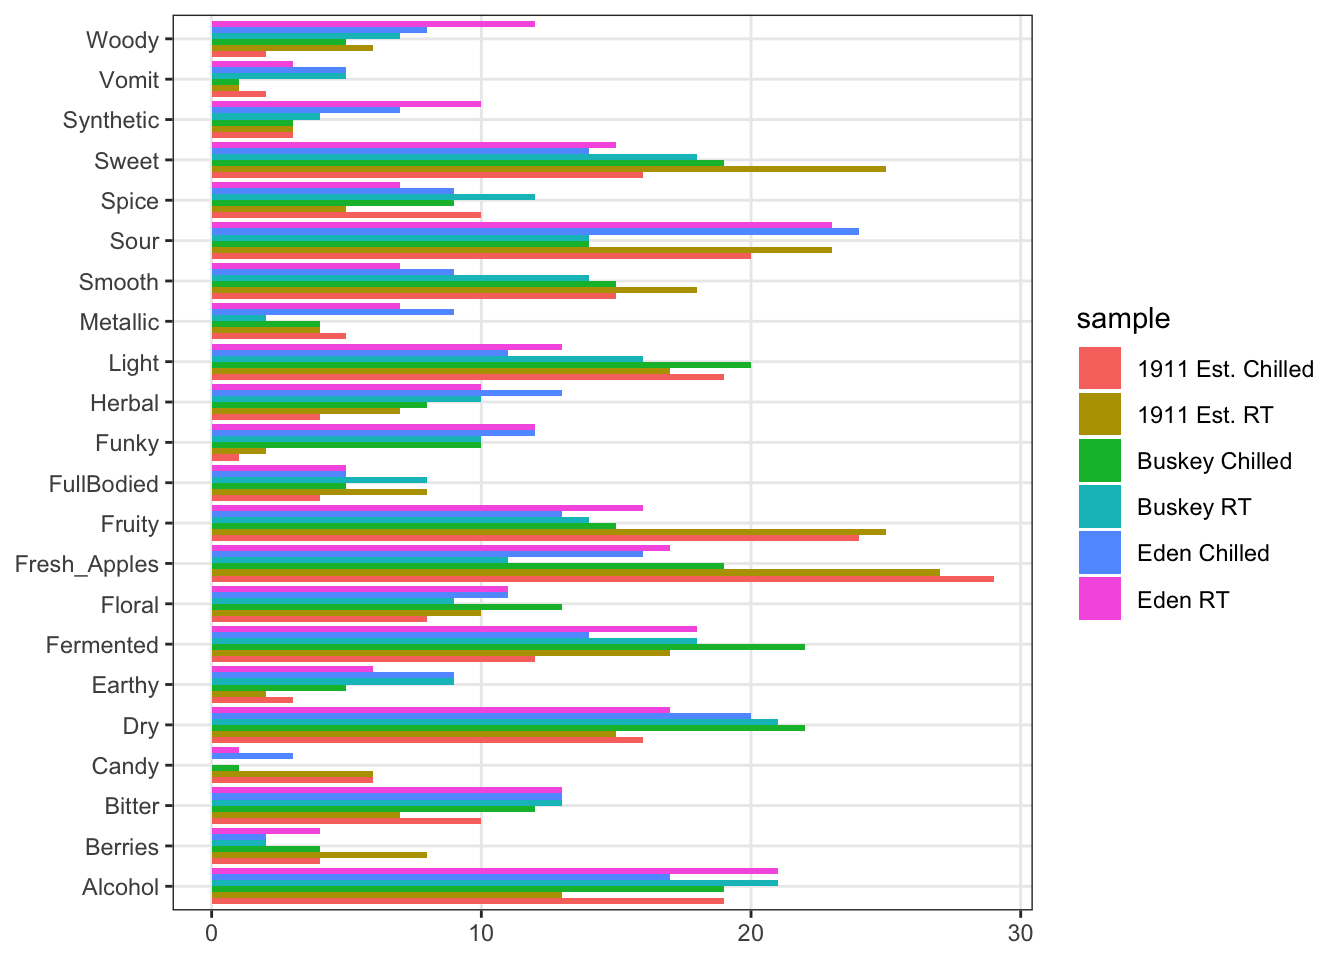
\includegraphics{02-import-wrangle-export_files/figure-latex/unnamed-chunk-2-1} \end{center}

Like I said, we're not here to tell you \emph{how} your plots should look\ldots{}

The motivating point, here, is to be able to make visualizations that accomplish what you want them to, rather than being at the mercy of packages that have certain defaults built in.

\hypertarget{getting-data-into-r}{%
\section{\texorpdfstring{Getting data into \texttt{R}}{Getting data into R}}\label{getting-data-into-r}}

Before we're able to analyze anything, we need to get data into \texttt{R}. In the workshop archive you downloaded, the \texttt{data/} directory has files called \texttt{clt-berry-data.csv} and \texttt{CiderDryness\_SensoryDATA.csv}. These are the files that hold the raw data.

\hypertarget{where-the-data-live}{%
\subsection{Where the data live}\label{where-the-data-live}}

To get these data into \texttt{R}, we need to briefly talk about \textbf{working directories} because this is how \texttt{R} ``sees'' your computer. It will look first in the working directory, and then you will have to tell it where the file is \emph{relative} to that directory. If you have been following along and opened up the \texttt{.Rproj} file in the downloaded archive, your working directory should be the archive's top level, which will mean that we only need to point \texttt{R} towards the \texttt{data/} folder and then the \texttt{clt-berry-data.csv} file. We can check the working directory with the \texttt{getwd()} function.

\begin{Shaded}
\begin{Highlighting}[]
\FunctionTok{getwd}\NormalTok{()}
\end{Highlighting}
\end{Shaded}

\begin{verbatim}
## [1] "C:/Users/lhamilton/Documents/sensometrics-r-tutorial-2024"
\end{verbatim}

Therefore, \textbf{relative to the working directory}, the file path to this data is \texttt{data/clt-berry-data.csv}. Please note that this is the UNIX convention for file paths: in Windows, the backslash \texttt{\textbackslash{}} is used to separate directories. Happily, RStudio will translate between the two conventions, so you can just follow along with the macOS/UNIX convention (\texttt{/}) in this workshop.

\hypertarget{getting-different-kinds-of-files-into-r}{%
\subsection{\texorpdfstring{Getting different kinds of files into \texttt{R}}{Getting different kinds of files into R}}\label{getting-different-kinds-of-files-into-r}}

The first step is to notice this is a \texttt{.csv} file, which stands for \textbf{c}omma-\textbf{s}eparated \textbf{v}alue. This means our data, in raw format, looks something like this:

\begin{verbatim}
# Comma-separated data (regarding Jake's cats)

cat_acquisition_order,name,weight,age\n
1,Nick,9,17\n
2,Margot,7,16\n
3,Little Guy,13,4\n
\end{verbatim}

Each line represents a row of data, and each field is separated by a comma (\texttt{,}). We can read this kind of data into \texttt{R} by using the \texttt{read\_csv()} function (this is a nicer version of the default \texttt{read.csv()} function, and we get access to it by loading \texttt{tidyverse} with \texttt{library(tidyverse)}).

\begin{Shaded}
\begin{Highlighting}[]
\FunctionTok{read\_csv}\NormalTok{(}\AttributeTok{file =} \StringTok{"data/clt{-}berry{-}data.csv"}\NormalTok{)}
\end{Highlighting}
\end{Shaded}

\begin{verbatim}
## Rows: 7507 Columns: 92
## -- Column specification --------------------------------------------------------
## Delimiter: ","
## chr  (7): Start Time (UTC), End Time (UTC), Sample Name, verbal_likes, verba...
## dbl (83): Subject Code, Participant Name, Serving Position, Sample Identifie...
## lgl  (2): Gender, Age
## 
## i Use `spec()` to retrieve the full column specification for this data.
## i Specify the column types or set `show_col_types = FALSE` to quiet this message.
\end{verbatim}

\begin{verbatim}
## # A tibble: 7,507 x 92
##    `Subject Code` `Participant Name` Gender Age   `Start Time (UTC)`
##             <dbl>              <dbl> <lgl>  <lgl> <chr>             
##  1           1001               1001 NA     NA    6/13/2019 21:05   
##  2           1001               1001 NA     NA    6/13/2019 20:55   
##  3           1001               1001 NA     NA    6/13/2019 20:49   
##  4           1001               1001 NA     NA    6/13/2019 20:45   
##  5           1001               1001 NA     NA    6/13/2019 21:00   
##  6           1001               1001 NA     NA    6/13/2019 21:10   
##  7           1002               1002 NA     NA    6/13/2019 20:08   
##  8           1002               1002 NA     NA    6/13/2019 19:57   
##  9           1002               1002 NA     NA    6/13/2019 20:13   
## 10           1002               1002 NA     NA    6/13/2019 20:03   
## # i 7,497 more rows
## # i 87 more variables: `End Time (UTC)` <chr>, `Serving Position` <dbl>,
## #   `Sample Identifier` <dbl>, `Sample Name` <chr>, `9pt_appearance` <dbl>,
## #   pre_expectation <dbl>, jar_color <dbl>, jar_gloss <dbl>, jar_size <dbl>,
## #   cata_appearance_unevencolor <dbl>, cata_appearance_misshapen <dbl>,
## #   cata_appearance_creased <dbl>, cata_appearance_seedy <dbl>,
## #   cata_appearance_bruised <dbl>, cata_appearance_notfresh <dbl>, ...
\end{verbatim}

\begin{Shaded}
\begin{Highlighting}[]
\FunctionTok{read\_csv}\NormalTok{(}\AttributeTok{file =} \StringTok{"data/CiderDryness\_SensoryDATA.csv"}\NormalTok{)}
\end{Highlighting}
\end{Shaded}

\begin{verbatim}
## Rows: 288 Columns: 27
## -- Column specification --------------------------------------------------------
## Delimiter: ","
## chr  (3): Sample_Name, Temperature, Panelist_Code
## dbl (24): MerlynScale_Ranking, Fresh_Apples, Fermented, Herbal, Dry, Spice, ...
## 
## i Use `spec()` to retrieve the full column specification for this data.
## i Specify the column types or set `show_col_types = FALSE` to quiet this message.
\end{verbatim}

\begin{verbatim}
## # A tibble: 288 x 27
##    Sample_Name Temperature Panelist_Code MerlynScale_Ranking Fresh_Apples
##    <chr>       <chr>       <chr>                       <dbl>        <dbl>
##  1 1911 Est.   Chilled     001                           2.3            1
##  2 Buskey      Chilled     001                           3.5            1
##  3 Eden        Chilled     001                           2.8            0
##  4 1911 Est.   RT          001                           4.2            0
##  5 Buskey      RT          001                           2              0
##  6 Eden        RT          001                           4              0
##  7 1911 Est.   Chilled     002                           3              1
##  8 Buskey      Chilled     002                           3.3            0
##  9 Eden        Chilled     002                           3.5            1
## 10 1911 Est.   RT          002                           4.5            0
## # i 278 more rows
## # i 22 more variables: Fermented <dbl>, Herbal <dbl>, Dry <dbl>, Spice <dbl>,
## #   Fruity <dbl>, Smooth <dbl>, Alcohol <dbl>, Light <dbl>, Sweet <dbl>,
## #   Woody <dbl>, Berries <dbl>, Sour <dbl>, Funky <dbl>, FullBodied <dbl>,
## #   Metallic <dbl>, Floral <dbl>, Candy <dbl>, Bitter <dbl>, Vomit <dbl>,
## #   Earthy <dbl>, Synthetic <dbl>, Liking <dbl>
\end{verbatim}

Remember that we need to store objects in the Environment if we want to access and modify them. Therefore, we need to remember to store these somewhere.

\begin{Shaded}
\begin{Highlighting}[]
\NormalTok{raw\_berry\_data }\OtherTok{\textless{}{-}} \FunctionTok{read\_csv}\NormalTok{(}\AttributeTok{file =} \StringTok{"data/clt{-}berry{-}data.csv"}\NormalTok{)}
\NormalTok{raw\_cider\_data }\OtherTok{\textless{}{-}} \FunctionTok{read\_csv}\NormalTok{(}\AttributeTok{file =} \StringTok{"data/CiderDryness\_SensoryDATA.csv"}\NormalTok{)}
\end{Highlighting}
\end{Shaded}

As a note, in many countries the separator (delimiter) will be the semi-colon (\texttt{;}), since the comma is used as the decimal marker. To read files formatted this way, you can use the \texttt{read\_csv2()} function. If you encounter tab-separated values files (\texttt{.tsv}) you can use the \texttt{read\_tsv()} function. If you have more non-standard delimiters, you can use the \texttt{read\_delim()} function, which will allow you to specify your own delimiter characters. Excel stores data by default in the \texttt{.xlsx} format, which can be read by installing and using the \texttt{readxl} package (or saving Excel data as \texttt{.csv}). You can also read many other formats of tabular data using the \texttt{rio} package (``read input/output''), which can be installed from CRAN (using, as you have learned, \texttt{install.packages("rio")}).

The \texttt{read\_csv()} function creates a type of object in \texttt{R} called a \texttt{tibble}, which is a special type of \texttt{data.frame}. These are rectangular ``spreadsheet-like'' objects like you would encounter in Excel or manipulate in JMP or SPSS.

We can learn more about the objects we just created by either examining them in the \texttt{Environment} tab or, preferably, using the \texttt{glimpse()} function to get a look at what we have (note that \texttt{glimpse()} comes from \texttt{tidyverse}; if you don't load it by running \texttt{library(tidyverse)} earlier in your session you will get an error).

\begin{Shaded}
\begin{Highlighting}[]
\FunctionTok{glimpse}\NormalTok{(raw\_berry\_data)}
\end{Highlighting}
\end{Shaded}

\begin{verbatim}
## Rows: 7,507
## Columns: 92
## $ `Subject Code`              <dbl> 1001, 1001, 1001, 1001, 1001, 1001, 1002, ~
## $ `Participant Name`          <dbl> 1001, 1001, 1001, 1001, 1001, 1001, 1002, ~
## $ Gender                      <lgl> NA, NA, NA, NA, NA, NA, NA, NA, NA, NA, NA~
## $ Age                         <lgl> NA, NA, NA, NA, NA, NA, NA, NA, NA, NA, NA~
## $ `Start Time (UTC)`          <chr> "6/13/2019 21:05", "6/13/2019 20:55", "6/1~
## $ `End Time (UTC)`            <chr> "6/13/2019 21:09", "6/13/2019 20:59", "6/1~
## $ `Serving Position`          <dbl> 5, 3, 2, 1, 4, 6, 3, 1, 4, 2, 6, 5, 2, 4, ~
## $ `Sample Identifier`         <dbl> 1426, 3167, 4624, 5068, 7195, 9161, 1426, ~
## $ `Sample Name`               <chr> "raspberry 6", "raspberry 5", "raspberry 2~
## $ `9pt_appearance`            <dbl> 4, 8, 4, 7, 7, 7, 6, 8, 8, 7, 9, 8, 5, 5, ~
## $ pre_expectation             <dbl> 2, 4, 2, 4, 3, 4, 2, 3, 5, 3, 4, 5, 3, 3, ~
## $ jar_color                   <dbl> 2, 3, 2, 2, 4, 4, 2, 3, 3, 2, 3, 4, 3, 3, ~
## $ jar_gloss                   <dbl> 4, 3, 2, 3, 3, 3, 4, 3, 4, 4, 2, 4, 3, 3, ~
## $ jar_size                    <dbl> 2, 3, 3, 4, 3, 3, 4, 3, 5, 3, 3, 4, 3, 3, ~
## $ cata_appearance_unevencolor <dbl> 0, 0, 0, 0, 1, 0, 0, 1, 1, 1, 0, 0, 0, 0, ~
## $ cata_appearance_misshapen   <dbl> 1, 0, 0, 0, 1, 0, 0, 0, 0, 0, 0, 0, 1, 1, ~
## $ cata_appearance_creased     <dbl> 0, 0, 0, 0, 0, 0, 0, 0, 1, 1, 0, 0, 1, 1, ~
## $ cata_appearance_seedy       <dbl> 0, 0, 0, 0, 0, 0, 0, 0, 0, 0, 0, 0, 0, 0, ~
## $ cata_appearance_bruised     <dbl> 0, 0, 0, 0, 0, 0, 0, 0, 1, 1, 0, 0, 0, 1, ~
## $ cata_appearance_notfresh    <dbl> 1, 0, 1, 0, 0, 0, 0, 0, 0, 0, 0, 0, 1, 1, ~
## $ cata_appearance_fresh       <dbl> 0, 1, 0, 1, 0, 1, 1, 1, 1, 1, 1, 1, 0, 0, ~
## $ cata_appearance_goodshape   <dbl> 0, 1, 0, 1, 0, 1, 1, 1, 0, 0, 1, 1, 0, 0, ~
## $ cata_appearance_goodquality <dbl> 0, 1, 0, 1, 0, 1, 1, 1, 1, 0, 1, 1, 1, 0, ~
## $ cata_appearance_none        <dbl> 0, 0, 0, 0, 0, 0, 0, 0, 0, 0, 0, 0, 0, 0, ~
## $ `9pt_overall`               <dbl> 4, 9, 3, 7, 4, 4, 4, 7, 7, 9, 7, 2, 8, 7, ~
## $ verbal_likes                <chr> "Out of the two, there was one that had a ~
## $ verbal_dislikes             <chr> "There were different flavors coming from ~
## $ `9pt_taste`                 <dbl> 4, 9, 3, 6, 3, 3, 4, 4, 6, 9, 6, 2, 8, 7, ~
## $ grid_sweetness              <dbl> 3, 6, 3, 6, 2, 3, 3, 2, 2, 6, 4, 1, 6, 4, ~
## $ grid_tartness               <dbl> 6, 5, 5, 3, 5, 6, 5, 5, 5, 2, 2, 7, 4, 5, ~
## $ grid_raspberryflavor        <dbl> 4, 7, 2, 6, 2, 3, 2, 6, 2, 7, 2, 2, 6, 5, ~
## $ jar_sweetness               <dbl> 2, 3, 2, 3, 2, 1, 1, 1, 1, 3, 2, 1, 3, 3, ~
## $ jar_tartness                <dbl> 4, 3, 3, 3, 4, 5, 4, 4, 4, 3, 4, 5, 3, 3, ~
## $ cata_taste_floral           <dbl> 0, 0, 0, 1, 0, 0, 0, 1, 1, 1, 1, 0, 0, 0, ~
## $ cata_taste_berry            <dbl> 1, 1, 0, 1, 0, 0, 0, 1, 0, 1, 0, 0, 1, 1, ~
## $ cata_taste_green            <dbl> 0, 0, 0, 1, 1, 1, 0, 0, 1, 0, 0, 1, 0, 0, ~
## $ cata_taste_grassy           <dbl> 0, 0, 0, 0, 1, 1, 1, 0, 1, 0, 1, 1, 0, 1, ~
## $ cata_taste_fermented        <dbl> 0, 0, 1, 0, 0, 0, 0, 0, 0, 0, 0, 0, 0, 0, ~
## $ cata_taste_tropical         <dbl> 1, 1, 0, 0, 0, 0, 0, 0, 0, 1, 0, 0, 1, 1, ~
## $ cata_taste_fruity           <dbl> 1, 1, 0, 1, 0, 0, 0, 0, 0, 1, 0, 0, 1, 0, ~
## $ cata_taste_citrus           <dbl> 1, 0, 0, 0, 0, 1, 1, 0, 0, 0, 1, 0, 1, 1, ~
## $ cata_taste_earthy           <dbl> 0, 0, 0, 0, 1, 0, 0, 1, 0, 0, 0, 1, 0, 0, ~
## $ cata_taste_candy            <dbl> 0, 0, 1, 0, 0, 0, 0, 0, 0, 0, 0, 0, 1, 0, ~
## $ cata_taste_none             <dbl> 0, 0, 0, 0, 0, 0, 0, 0, 0, 0, 0, 0, 0, 0, ~
## $ `9pt_texture`               <dbl> 6, 8, 2, 8, 5, 6, 6, 9, 8, 7, 7, 7, 8, 7, ~
## $ grid_seediness              <dbl> 3, 5, 6, 3, 5, 5, 6, 4, 6, 5, 6, 5, 4, 4, ~
## $ grid_firmness               <dbl> 5, 5, 5, 2, 6, 5, 5, 6, 5, 3, 5, 5, 4, 5, ~
## $ grid_juiciness              <dbl> 2, 5, 2, 2, 2, 4, 2, 4, 2, 3, 3, 2, 6, 5, ~
## $ jar_firmness                <dbl> 3, 3, 4, 2, 4, 3, 3, 3, 3, 2, 3, 3, 3, 3, ~
## $ jar_juciness                <dbl> 2, 3, 1, 2, 2, 2, 1, 2, 1, 3, 2, 1, 3, 3, ~
## $ post_expectation            <dbl> 1, 5, 2, 4, 2, 2, 2, 2, 2, 5, 2, 1, 4, 3, ~
## $ price                       <dbl> 1.99, 4.99, 2.99, 4.99, 2.99, 3.99, 3.99, ~
## $ product_tier                <dbl> 1, 3, 2, 3, 1, 2, 2, 2, 1, 3, 2, 1, 2, 2, ~
## $ purchase_intent             <dbl> 1, 5, 2, 4, 2, 2, 3, 4, 2, 5, 3, 1, 5, 5, ~
## $ subject                     <dbl> 1031946, 1031946, 1031946, 1031946, 103194~
## $ test_day                    <chr> "Raspberry Day 1", "Raspberry Day 1", "Ras~
## $ us_appearance               <dbl> NA, NA, NA, NA, NA, NA, NA, NA, NA, NA, NA~
## $ us_overall                  <dbl> NA, NA, NA, NA, NA, NA, NA, NA, NA, NA, NA~
## $ us_taste                    <dbl> NA, NA, NA, NA, NA, NA, NA, NA, NA, NA, NA~
## $ us_texture                  <dbl> NA, NA, NA, NA, NA, NA, NA, NA, NA, NA, NA~
## $ lms_appearance              <dbl> NA, NA, NA, NA, NA, NA, NA, NA, NA, NA, NA~
## $ lms_overall                 <dbl> NA, NA, NA, NA, NA, NA, NA, NA, NA, NA, NA~
## $ lms_taste                   <dbl> NA, NA, NA, NA, NA, NA, NA, NA, NA, NA, NA~
## $ lms_texture                 <dbl> NA, NA, NA, NA, NA, NA, NA, NA, NA, NA, NA~
## $ cata_appearane_bruised      <dbl> NA, NA, NA, NA, NA, NA, NA, NA, NA, NA, NA~
## $ cata_appearance_goodshapre  <dbl> NA, NA, NA, NA, NA, NA, NA, NA, NA, NA, NA~
## $ cata_appearance_goodcolor   <dbl> NA, NA, NA, NA, NA, NA, NA, NA, NA, NA, NA~
## $ grid_blackberryflavor       <dbl> NA, NA, NA, NA, NA, NA, NA, NA, NA, NA, NA~
## $ cata_taste_cinnamon         <dbl> NA, NA, NA, NA, NA, NA, NA, NA, NA, NA, NA~
## $ cata_taste_lemon            <dbl> NA, NA, NA, NA, NA, NA, NA, NA, NA, NA, NA~
## $ cata_taste_clove            <dbl> NA, NA, NA, NA, NA, NA, NA, NA, NA, NA, NA~
## $ cata_taste_minty            <dbl> NA, NA, NA, NA, NA, NA, NA, NA, NA, NA, NA~
## $ cata_taste_grape            <dbl> NA, NA, NA, NA, NA, NA, NA, NA, NA, NA, NA~
## $ grid_crispness              <dbl> NA, NA, NA, NA, NA, NA, NA, NA, NA, NA, NA~
## $ jar_crispness               <dbl> NA, NA, NA, NA, NA, NA, NA, NA, NA, NA, NA~
## $ jar_juiciness               <dbl> NA, NA, NA, NA, NA, NA, NA, NA, NA, NA, NA~
## $ cata_appearane_creased      <dbl> NA, NA, NA, NA, NA, NA, NA, NA, NA, NA, NA~
## $ grid_blueberryflavor        <dbl> NA, NA, NA, NA, NA, NA, NA, NA, NA, NA, NA~
## $ cata_taste_piney            <dbl> NA, NA, NA, NA, NA, NA, NA, NA, NA, NA, NA~
## $ cata_taste_peachy           <dbl> NA, NA, NA, NA, NA, NA, NA, NA, NA, NA, NA~
## $ `9pt_aroma`                 <dbl> NA, NA, NA, NA, NA, NA, NA, NA, NA, NA, NA~
## $ grid_strawberryflavor       <dbl> NA, NA, NA, NA, NA, NA, NA, NA, NA, NA, NA~
## $ cata_taste_caramel          <dbl> NA, NA, NA, NA, NA, NA, NA, NA, NA, NA, NA~
## $ cata_taste_grapey           <dbl> NA, NA, NA, NA, NA, NA, NA, NA, NA, NA, NA~
## $ cata_taste_melon            <dbl> NA, NA, NA, NA, NA, NA, NA, NA, NA, NA, NA~
## $ cata_taste_cherry           <dbl> NA, NA, NA, NA, NA, NA, NA, NA, NA, NA, NA~
## $ grid_crunchiness            <dbl> NA, NA, NA, NA, NA, NA, NA, NA, NA, NA, NA~
## $ jar_crunch                  <dbl> NA, NA, NA, NA, NA, NA, NA, NA, NA, NA, NA~
## $ us_aroma                    <dbl> NA, NA, NA, NA, NA, NA, NA, NA, NA, NA, NA~
## $ lms_aroma                   <dbl> NA, NA, NA, NA, NA, NA, NA, NA, NA, NA, NA~
## $ berry                       <chr> "raspberry", "raspberry", "raspberry", "ra~
## $ sample                      <dbl> 6, 5, 2, 3, 4, 1, 6, 5, 2, 3, 4, 1, 6, 5, ~
\end{verbatim}

\begin{Shaded}
\begin{Highlighting}[]
\FunctionTok{glimpse}\NormalTok{(raw\_cider\_data)}
\end{Highlighting}
\end{Shaded}

\begin{verbatim}
## Rows: 288
## Columns: 27
## $ Sample_Name         <chr> "1911 Est.", "Buskey", "Eden", "1911 Est.", "Buske~
## $ Temperature         <chr> "Chilled", "Chilled", "Chilled", "RT", "RT", "RT",~
## $ Panelist_Code       <chr> "001", "001", "001", "001", "001", "001", "002", "~
## $ MerlynScale_Ranking <dbl> 2.3, 3.5, 2.8, 4.2, 2.0, 4.0, 3.0, 3.3, 3.5, 4.5, ~
## $ Fresh_Apples        <dbl> 1, 1, 0, 0, 0, 0, 1, 0, 1, 0, 0, 1, 1, 0, 0, 0, 0,~
## $ Fermented           <dbl> 0, 1, 0, 1, 1, 1, 1, 0, 0, 0, 0, 1, 0, 1, 0, 0, 0,~
## $ Herbal              <dbl> 0, 0, 1, 0, 1, 0, 0, 0, 0, 0, 0, 0, 0, 0, 1, 0, 1,~
## $ Dry                 <dbl> 1, 1, 0, 0, 1, 1, 0, 0, 0, 0, 0, 0, 0, 0, 0, 0, 0,~
## $ Spice               <dbl> 0, 0, 0, 0, 1, 0, 0, 0, 0, 0, 0, 0, 0, 0, 0, 0, 0,~
## $ Fruity              <dbl> 0, 0, 0, 0, 0, 0, 0, 1, 0, 0, 0, 0, 0, 0, 0, 1, 1,~
## $ Smooth              <dbl> 0, 0, 0, 0, 0, 0, 0, 0, 0, 0, 0, 0, 0, 0, 0, 0, 0,~
## $ Alcohol             <dbl> 0, 0, 0, 0, 0, 0, 0, 0, 0, 0, 0, 0, 0, 0, 0, 0, 0,~
## $ Light               <dbl> 0, 0, 0, 0, 0, 1, 1, 1, 0, 0, 0, 0, 0, 0, 0, 0, 1,~
## $ Sweet               <dbl> 0, 1, 0, 1, 1, 1, 0, 0, 0, 0, 0, 0, 1, 0, 1, 1, 0,~
## $ Woody               <dbl> 1, 0, 0, 0, 0, 0, 0, 0, 0, 0, 0, 0, 0, 0, 0, 0, 0,~
## $ Berries             <dbl> 1, 0, 0, 0, 0, 0, 0, 0, 0, 0, 0, 0, 0, 0, 0, 0, 0,~
## $ Sour                <dbl> 1, 1, 1, 1, 1, 1, 1, 0, 1, 0, 0, 0, 1, 0, 0, 0, 0,~
## $ Funky               <dbl> 0, 0, 1, 1, 1, 0, 0, 0, 0, 0, 1, 0, 0, 0, 0, 0, 0,~
## $ FullBodied          <dbl> 0, 0, 0, 0, 0, 0, 0, 0, 0, 0, 1, 0, 0, 0, 0, 0, 0,~
## $ Metallic            <dbl> 1, 0, 0, 1, 0, 0, 0, 0, 0, 0, 0, 1, 0, 0, 0, 0, 0,~
## $ Floral              <dbl> 0, 0, 0, 0, 0, 1, 0, 0, 0, 0, 0, 0, 0, 1, 1, 0, 0,~
## $ Candy               <dbl> 0, 0, 0, 0, 0, 0, 0, 0, 0, 0, 0, 0, 0, 0, 0, 1, 0,~
## $ Bitter              <dbl> 0, 0, 0, 0, 0, 1, 0, 0, 0, 0, 0, 0, 0, 0, 0, 0, 0,~
## $ Vomit               <dbl> 0, 0, 1, 1, 1, 0, 0, 0, 0, 0, 0, 0, 0, 0, 0, 0, 0,~
## $ Earthy              <dbl> 1, 0, 1, 0, 1, 0, 0, 0, 0, 0, 0, 0, 0, 0, 0, 0, 0,~
## $ Synthetic           <dbl> 0, 0, 0, 1, 0, 1, 0, 0, 0, 1, 0, 0, 0, 0, 0, 0, 0,~
## $ Liking              <dbl> 6, 7, 4, 2, 7, 5, 8, 6, 7, 3, 4, 4, 7, 6, 5, 6, 4,~
\end{verbatim}

This tells us how many rows we have, what the names of our columns (variables) are, what kind of column they are (numeric, character, logical, etc), and a preview of the first few entres in each column.

\hypertarget{wrangling-selecting-filtering-reshaping-data}{%
\section{Wrangling (selecting, filtering, reshaping) data}\label{wrangling-selecting-filtering-reshaping-data}}

Our students often tell us that the hardest part of data analysis and visualization is getting data into the tool you want to use (here \texttt{R}) and into the right ``shape'' for the relevant analysis. We tend to agree: a common saying in data science is that about 90\% of the effort in an analysis workflow is in getting data wrangled into the right format and shape, and 10\% is actual analysis. In a point and click program like SPSS or XLSTAT we don't think about this as much because the activity of reshaping the data--making it longer or wider as required, finding and cleaning missing values, selecting columns or rows, etc--is often temporally and programmatically separated from the ``actual'' analysis.

In \texttt{R}, this can feel a bit different because we are using the same interface to manipulate our data and to analyze it. Sometimes we'll want to jump back out to a spreadsheet program like Excel or even the command line (the ``shell'' like \texttt{bash} or \texttt{zsh}) to make some changes. But in general the tools for manipulating data in \texttt{R} are both more powerful and more easily used than doing these activities by hand, and you will make yourself a much more effective analyst by mastering these basic tools.

Here, we are going to emphasize the set of tools from the \href{https://www.tidyverse.org/}{\texttt{tidyverse}}, which are extensively documented in Hadley Wickham and Garrett Grolemund's book \href{https://r4ds.had.co.nz/}{\emph{R for Data Science}}. If you want to learn more, start there!

\begin{figure}
\centering
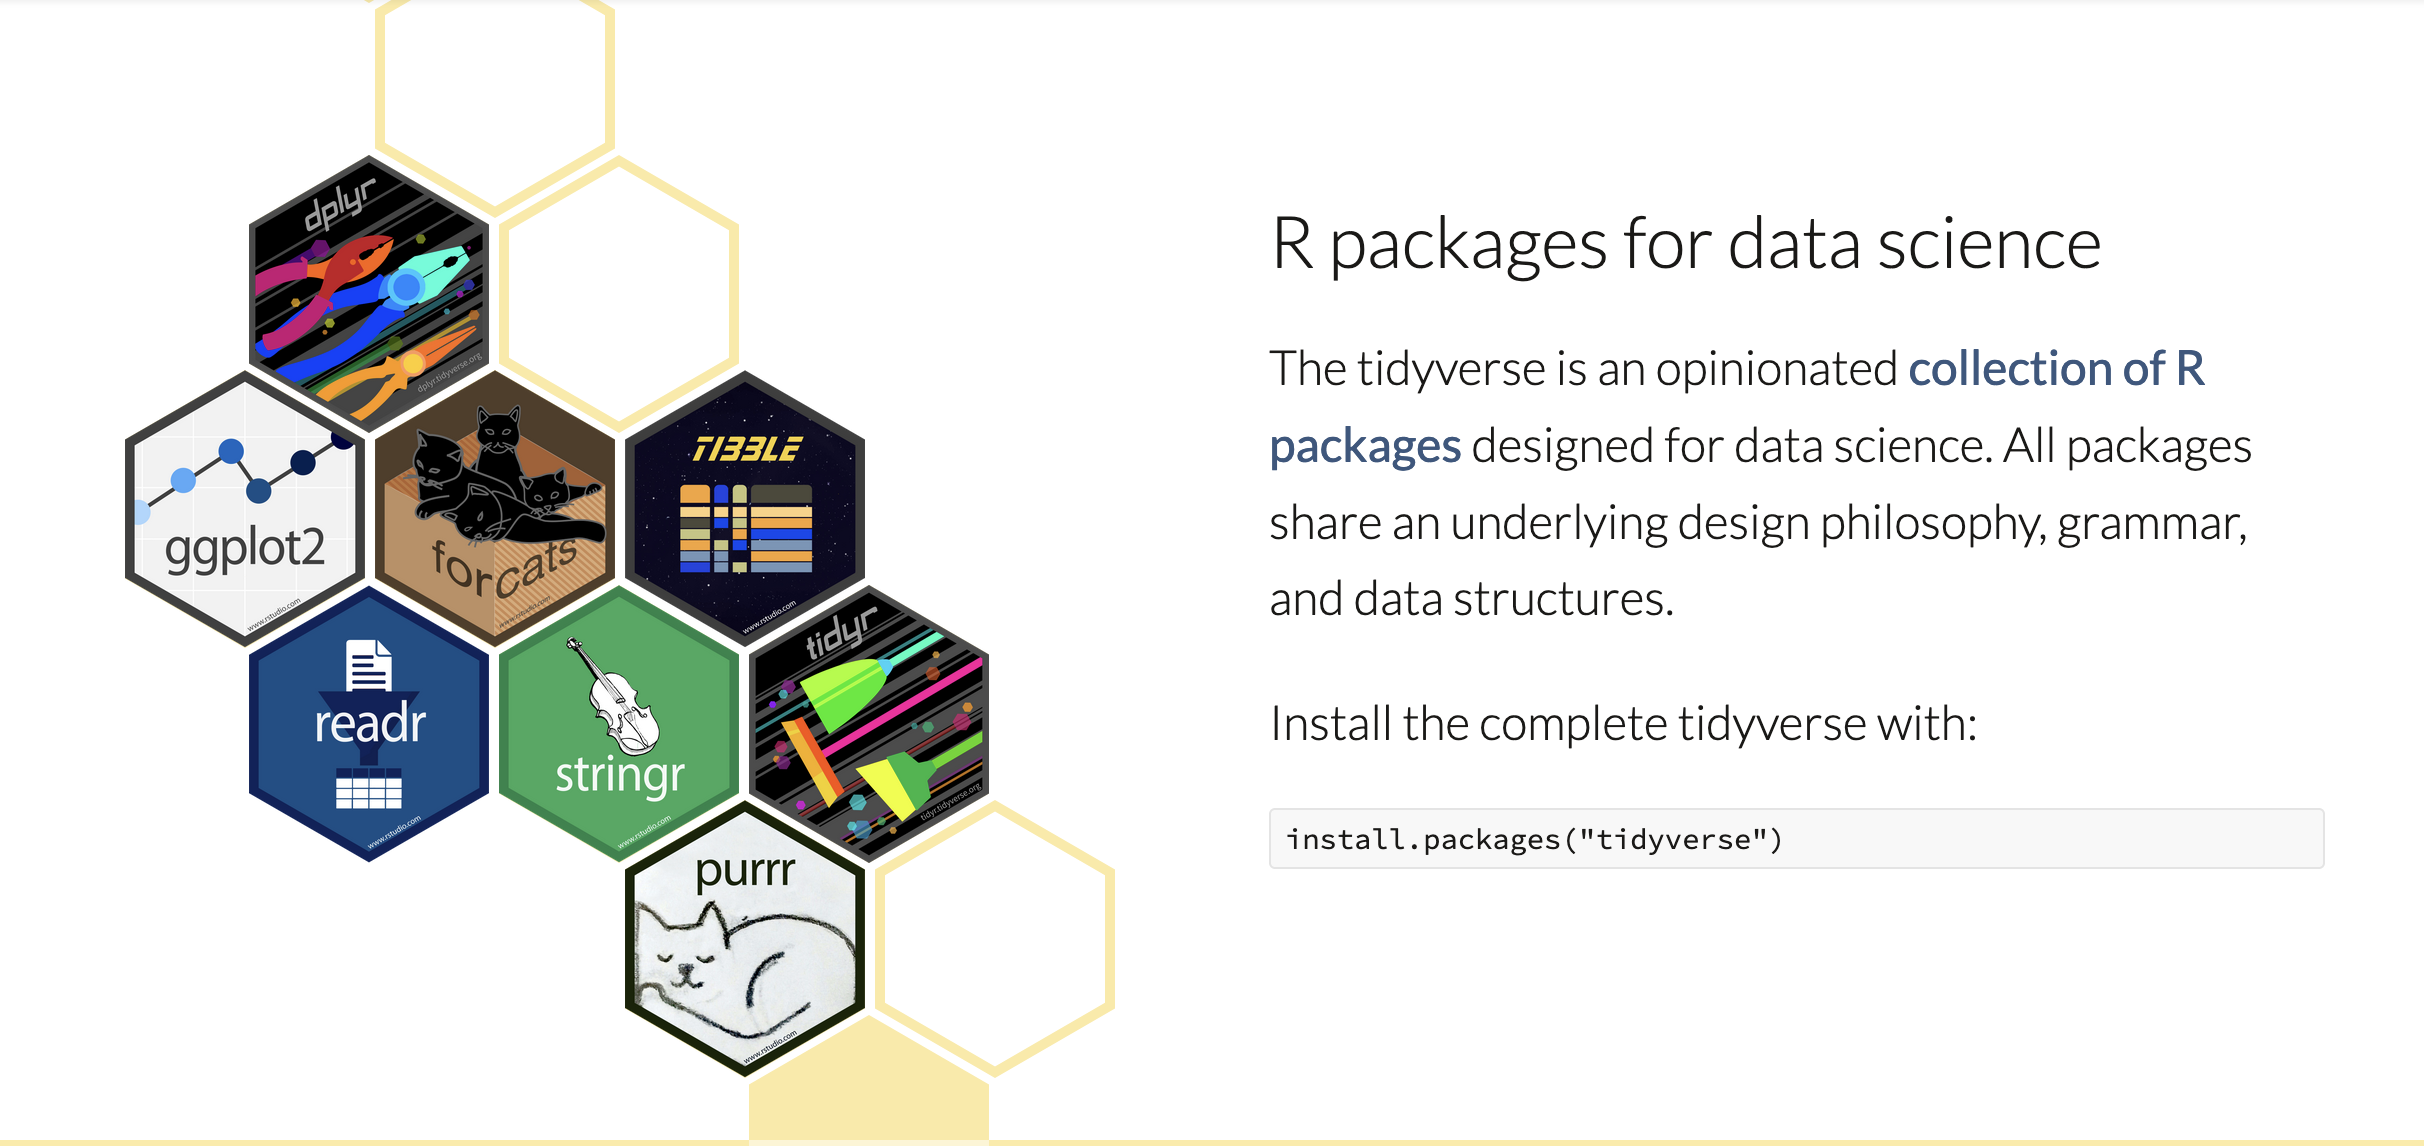
\includegraphics{img/tidyverse-iconography.png}
\caption{The \texttt{tidyverse} is associated with this hexagonal iconography.}
\end{figure}

If you're at all familiar with \texttt{R}, you will have learned about subsetting \texttt{R} objects like lists and data frames using operators like \texttt{{[}} or \texttt{{[}{[}} and logical comparisons like \texttt{x\ \textless{}\ 10}. If you are used to code conventions, this is a great system! However, for people who are less familiar with coding, these are often difficult to parse and to remember. So in this workshop we're going to assume you've been exposed to this information, and we're not going to use or focus on it very much; instead, we're going to look at the tools within the \texttt{tidyverse} that accomplish the same things in--we think!--a much easier to parse and remember fashion.

\hypertarget{the-pipe-for-multiple-steps-in-a-workflow}{%
\subsection{\texorpdfstring{The ``pipe'' for multiple steps in a workflow: \texttt{\%\textgreater{}\%}}{The ``pipe'' for multiple steps in a workflow: \%\textgreater\%}}\label{the-pipe-for-multiple-steps-in-a-workflow}}

While I am not going to go over much of the base \texttt{R} syntax, I want to talk about one particular tool that is becoming standard in modern \texttt{R} coding: the \textbf{pipe}, which is written in \texttt{tidyverse} as \texttt{\%\textgreater{}\%}. This garbage-looking set of symbols is actually your best friend, you just don't know it yet. I use this tool constantly in my R programming.

OK, enough background, what the heck \emph{is} a pipe? The term ``pipe'' comes from what it does: like a pipe, \texttt{\%\textgreater{}\%} lets whatever is on its left side flow through to the right hand side. It is easiest to read \texttt{\%\textgreater{}\%} as ``\textbf{AND THEN}''.

\begin{Shaded}
\begin{Highlighting}[]
\NormalTok{raw\_berry\_data }\SpecialCharTok{\%\textgreater{}\%}                         \CommentTok{\# Start with the berry\_data}
  \FunctionTok{filter}\NormalTok{(berry }\SpecialCharTok{==} \StringTok{"blackberry"}\NormalTok{) }\SpecialCharTok{\%\textgreater{}\%}        \CommentTok{\# AND THEN filter to blackberries}
  \FunctionTok{select}\NormalTok{(}\StringTok{\textasciigrave{}}\AttributeTok{Sample Name}\StringTok{\textasciigrave{}}\NormalTok{,                    }\CommentTok{\# AND THEN select sample name, overall liking...}
         \FunctionTok{contains}\NormalTok{(}\StringTok{"\_overall"}\NormalTok{), }
         \FunctionTok{contains}\NormalTok{(}\StringTok{"cata\_"}\NormalTok{))}
\end{Highlighting}
\end{Shaded}

\begin{verbatim}
## # A tibble: 1,495 x 40
##    `Sample Name` `9pt_overall` us_overall lms_overall cata_appearance_unevenco~1
##    <chr>                 <dbl>      <dbl>       <dbl>                      <dbl>
##  1 Blackberry 4              2         NA          NA                          0
##  2 Blackberry 2              5         NA          NA                          0
##  3 Blackberry 1              8         NA          NA                          0
##  4 Blackberry 3              6         NA          NA                          0
##  5 Blackberry 5              8         NA          NA                          0
##  6 Blackberry 4              6         NA          NA                          0
##  7 Blackberry 2              1         NA          NA                          0
##  8 Blackberry 1              8         NA          NA                          0
##  9 Blackberry 3              8         NA          NA                          0
## 10 Blackberry 5              8         NA          NA                          0
## # i 1,485 more rows
## # i abbreviated name: 1: cata_appearance_unevencolor
## # i 35 more variables: cata_appearance_misshapen <dbl>,
## #   cata_appearance_creased <dbl>, cata_appearance_seedy <dbl>,
## #   cata_appearance_bruised <dbl>, cata_appearance_notfresh <dbl>,
## #   cata_appearance_fresh <dbl>, cata_appearance_goodshape <dbl>,
## #   cata_appearance_goodquality <dbl>, cata_appearance_none <dbl>, ...
\end{verbatim}

Typing \texttt{\%\textgreater{}\%} is no fun. But, happily, RStudio builds in a shortcut for you: macOS is \texttt{cmd\ +\ shift\ +\ M}, Windows is \texttt{ctrl\ +\ shift\ +\ M}.

Please note that since \texttt{R} 4.1, a \emph{native} pipe has been implemented (you don't need to load \texttt{tidyverse} for it to work), which is written as \texttt{\textbar{}\textgreater{}}. If you are new to using pipes, you can pretty safely use either one that you prefer, and you can configure the keyboard shortcuts above to use either the native or \texttt{tidyverse} pipe. The default depends on your version of Rstudio. If you want to learn details, \href{https://www.tidyverse.org/blog/2023/04/base-vs-magrittr-pipe/}{this article is helpful}.

\textbf{TL;DR}: The pipe lets us quickly write functional workflows without saving a lot of intermediate steps. We're going to use it a lot in the following examples, and I'll call it out the first few times so that you can get the hang of it.

\hypertarget{subsetting-your-data}{%
\subsection{Subsetting your data}\label{subsetting-your-data}}

The first thing you'll notice about our \texttt{raw\_berry\_data} in particular is that it is \emph{full} of information we don't need! A common situation in R is wanting to select some rows and some columns of our data--this is called ``\textbf{subsetting}'' our data. But this is less easy than it might be for the beginner in R. Happily, the \texttt{tidverse} methods are much easier to read (and modeled after syntax from \textbf{SQL}, which may be helpful for some users).

\hypertarget{selecting-certain-columns-select}{%
\subsubsection{\texorpdfstring{Selecting certain columns: \texttt{select()}}{Selecting certain columns: select()}}\label{selecting-certain-columns-select}}

The first thing we did in our code to wrangle our \protect\hyperlink{berries}{\texttt{raw\_berry\_data}} into something useful was to determine that a number of columns were not necessary. We really only want the subject ID, the sample ID columns, and the CATA and the liking data. The rest of the data is either metadata (test date, etc) or other kinds of data that are not relevant to our analysis. We want to get rid of these.

The \texttt{tidyverse::select()} function (we write \texttt{{[}package{]}::{[}function{]}} to explicitly describe where a function comes from) lets us select columns in a rectangular data frame (like \texttt{.csv} and other spreadsheets) by name, position, or logical criteria. The subject ID is stored in a column called \texttt{Subject\ Code}, and the berry information is stored in two columns: \texttt{berry} and \texttt{sample}, indicating what kind of berry and what sample \# it is.

\begin{Shaded}
\begin{Highlighting}[]
\NormalTok{raw\_berry\_data }\SpecialCharTok{\%\textgreater{}\%}        \CommentTok{\# We start with our raw\_berry\_data frame}
  \FunctionTok{select}\NormalTok{(}\StringTok{\textasciigrave{}}\AttributeTok{Subject Code}\StringTok{\textasciigrave{}}\NormalTok{,  }\CommentTok{\# AND THEN we select these 3 columns}
\NormalTok{         berry,}
\NormalTok{         sample) }\SpecialCharTok{\%\textgreater{}\%}      \CommentTok{\# AND THEN we use glimpse() to get a quick summary}
  \FunctionTok{glimpse}\NormalTok{()}
\end{Highlighting}
\end{Shaded}

\begin{verbatim}
## Rows: 7,507
## Columns: 3
## $ `Subject Code` <dbl> 1001, 1001, 1001, 1001, 1001, 1001, 1002, 1002, 1002, 1~
## $ berry          <chr> "raspberry", "raspberry", "raspberry", "raspberry", "ra~
## $ sample         <dbl> 6, 5, 2, 3, 4, 1, 6, 5, 2, 3, 4, 1, 6, 5, 2, 3, 4, 1, 6~
\end{verbatim}

Now we only have these 3 columns!

\textbf{An aside:} Note the way that \texttt{Subject\ Code} is written: as \texttt{\textasciigrave{}Subject\ Code\textasciigrave{}}. This is because \texttt{R} will see some characters, including (but not limited to) white space (\texttt{}), leading numbers (starting with \texttt{1-9}), and special characters (like \texttt{,} or \texttt{:}), as indications that the variable name has ended. We can refer to these strange column names by using the \textbf{back-tick} operator \texttt{\textasciigrave{}} to escape the normal naming conventions. This happens often when, as we did here, we import data that wasn't made in \texttt{R}, like many \texttt{.csv} files. It is a pain to type back-ticks, but the \texttt{tab}-completion behavior we set up makes this easier.

To return to selection, we also want overall liking data and we want CATA variables. There are a lot of these, and typing them out individually in \texttt{select()} would be a pain. Luckily, there are a set of special functions for use within \texttt{select()} (and other \texttt{tidyverse} functions) that let us use logical operators to select ranges of columns/variables You can learn about them using the \texttt{?select} command to get the help file.

\begin{Shaded}
\begin{Highlighting}[]
\NormalTok{berry\_columns }\OtherTok{\textless{}{-}} 
\NormalTok{  raw\_berry\_data }\SpecialCharTok{\%\textgreater{}\%}
  \FunctionTok{select}\NormalTok{(}\StringTok{\textasciigrave{}}\AttributeTok{Subject Code}\StringTok{\textasciigrave{}}\NormalTok{,}
\NormalTok{         berry,}
\NormalTok{         sample,}
         \FunctionTok{starts\_with}\NormalTok{(}\StringTok{"cata"}\NormalTok{),    }\CommentTok{\# select columns whose names start with "cata"}
         \FunctionTok{contains}\NormalTok{(}\StringTok{"overall"}\NormalTok{))    }\CommentTok{\# select columns whose names contain "overall"}

\NormalTok{berry\_columns }\SpecialCharTok{\%\textgreater{}\%}
  \FunctionTok{glimpse}\NormalTok{()}
\end{Highlighting}
\end{Shaded}

\begin{verbatim}
## Rows: 7,507
## Columns: 42
## $ `Subject Code`              <dbl> 1001, 1001, 1001, 1001, 1001, 1001, 1002, ~
## $ berry                       <chr> "raspberry", "raspberry", "raspberry", "ra~
## $ sample                      <dbl> 6, 5, 2, 3, 4, 1, 6, 5, 2, 3, 4, 1, 6, 5, ~
## $ cata_appearance_unevencolor <dbl> 0, 0, 0, 0, 1, 0, 0, 1, 1, 1, 0, 0, 0, 0, ~
## $ cata_appearance_misshapen   <dbl> 1, 0, 0, 0, 1, 0, 0, 0, 0, 0, 0, 0, 1, 1, ~
## $ cata_appearance_creased     <dbl> 0, 0, 0, 0, 0, 0, 0, 0, 1, 1, 0, 0, 1, 1, ~
## $ cata_appearance_seedy       <dbl> 0, 0, 0, 0, 0, 0, 0, 0, 0, 0, 0, 0, 0, 0, ~
## $ cata_appearance_bruised     <dbl> 0, 0, 0, 0, 0, 0, 0, 0, 1, 1, 0, 0, 0, 1, ~
## $ cata_appearance_notfresh    <dbl> 1, 0, 1, 0, 0, 0, 0, 0, 0, 0, 0, 0, 1, 1, ~
## $ cata_appearance_fresh       <dbl> 0, 1, 0, 1, 0, 1, 1, 1, 1, 1, 1, 1, 0, 0, ~
## $ cata_appearance_goodshape   <dbl> 0, 1, 0, 1, 0, 1, 1, 1, 0, 0, 1, 1, 0, 0, ~
## $ cata_appearance_goodquality <dbl> 0, 1, 0, 1, 0, 1, 1, 1, 1, 0, 1, 1, 1, 0, ~
## $ cata_appearance_none        <dbl> 0, 0, 0, 0, 0, 0, 0, 0, 0, 0, 0, 0, 0, 0, ~
## $ cata_taste_floral           <dbl> 0, 0, 0, 1, 0, 0, 0, 1, 1, 1, 1, 0, 0, 0, ~
## $ cata_taste_berry            <dbl> 1, 1, 0, 1, 0, 0, 0, 1, 0, 1, 0, 0, 1, 1, ~
## $ cata_taste_green            <dbl> 0, 0, 0, 1, 1, 1, 0, 0, 1, 0, 0, 1, 0, 0, ~
## $ cata_taste_grassy           <dbl> 0, 0, 0, 0, 1, 1, 1, 0, 1, 0, 1, 1, 0, 1, ~
## $ cata_taste_fermented        <dbl> 0, 0, 1, 0, 0, 0, 0, 0, 0, 0, 0, 0, 0, 0, ~
## $ cata_taste_tropical         <dbl> 1, 1, 0, 0, 0, 0, 0, 0, 0, 1, 0, 0, 1, 1, ~
## $ cata_taste_fruity           <dbl> 1, 1, 0, 1, 0, 0, 0, 0, 0, 1, 0, 0, 1, 0, ~
## $ cata_taste_citrus           <dbl> 1, 0, 0, 0, 0, 1, 1, 0, 0, 0, 1, 0, 1, 1, ~
## $ cata_taste_earthy           <dbl> 0, 0, 0, 0, 1, 0, 0, 1, 0, 0, 0, 1, 0, 0, ~
## $ cata_taste_candy            <dbl> 0, 0, 1, 0, 0, 0, 0, 0, 0, 0, 0, 0, 1, 0, ~
## $ cata_taste_none             <dbl> 0, 0, 0, 0, 0, 0, 0, 0, 0, 0, 0, 0, 0, 0, ~
## $ cata_appearane_bruised      <dbl> NA, NA, NA, NA, NA, NA, NA, NA, NA, NA, NA~
## $ cata_appearance_goodshapre  <dbl> NA, NA, NA, NA, NA, NA, NA, NA, NA, NA, NA~
## $ cata_appearance_goodcolor   <dbl> NA, NA, NA, NA, NA, NA, NA, NA, NA, NA, NA~
## $ cata_taste_cinnamon         <dbl> NA, NA, NA, NA, NA, NA, NA, NA, NA, NA, NA~
## $ cata_taste_lemon            <dbl> NA, NA, NA, NA, NA, NA, NA, NA, NA, NA, NA~
## $ cata_taste_clove            <dbl> NA, NA, NA, NA, NA, NA, NA, NA, NA, NA, NA~
## $ cata_taste_minty            <dbl> NA, NA, NA, NA, NA, NA, NA, NA, NA, NA, NA~
## $ cata_taste_grape            <dbl> NA, NA, NA, NA, NA, NA, NA, NA, NA, NA, NA~
## $ cata_appearane_creased      <dbl> NA, NA, NA, NA, NA, NA, NA, NA, NA, NA, NA~
## $ cata_taste_piney            <dbl> NA, NA, NA, NA, NA, NA, NA, NA, NA, NA, NA~
## $ cata_taste_peachy           <dbl> NA, NA, NA, NA, NA, NA, NA, NA, NA, NA, NA~
## $ cata_taste_caramel          <dbl> NA, NA, NA, NA, NA, NA, NA, NA, NA, NA, NA~
## $ cata_taste_grapey           <dbl> NA, NA, NA, NA, NA, NA, NA, NA, NA, NA, NA~
## $ cata_taste_melon            <dbl> NA, NA, NA, NA, NA, NA, NA, NA, NA, NA, NA~
## $ cata_taste_cherry           <dbl> NA, NA, NA, NA, NA, NA, NA, NA, NA, NA, NA~
## $ `9pt_overall`               <dbl> 4, 9, 3, 7, 4, 4, 4, 7, 7, 9, 7, 2, 8, 7, ~
## $ us_overall                  <dbl> NA, NA, NA, NA, NA, NA, NA, NA, NA, NA, NA~
## $ lms_overall                 <dbl> NA, NA, NA, NA, NA, NA, NA, NA, NA, NA, NA~
\end{verbatim}

Because I am intimately familiar with these data, I know that all of the CATA variables were stored in columns starting with \texttt{"cata"}, and that ratings for overall acceptability were stored in columns that had \texttt{"overall"} somewhere in their name.

Unlike in our original workflow, we have created an intermediate data frame called \texttt{berry\_columns} to save us from repeating steps. But, as above in the original workflow, there is no reason we need to do this.

In our workflow above, note that our \protect\hyperlink{cider}{cider data} came to us pretty clean; we are not using \texttt{select()} anywhere to discard columns.

\hypertarget{filtering-certain-rows-filter}{%
\subsubsection{\texorpdfstring{Filtering certain rows: \texttt{filter()}}{Filtering certain rows: filter()}}\label{filtering-certain-rows-filter}}

Frequently we only want to select some of our observations, which are typically stored in the rows in our rectangular data frames. \texttt{select()} won't help us here, but its row-wise cousin, \texttt{filter()}, lets us filter down to only rows that meet some logical criteria. While you will notice that we do not use \texttt{filter()} on either the \protect\hyperlink{cider}{cider} or the \protect\hyperlink{berry}{berry} data above--we want to retain all of our observations in this case--it is easy to imagine situations in which we might want to only inspect a subset of our data.

For example, in the berry data, perhaps we want to separate out our observations on raspberries from all of our other data.

\begin{Shaded}
\begin{Highlighting}[]
\NormalTok{raw\_berry\_data }\SpecialCharTok{\%\textgreater{}\%}
  \FunctionTok{distinct}\NormalTok{(berry)                   }\CommentTok{\# distinct() gives all unique value combinations}
\end{Highlighting}
\end{Shaded}

\begin{verbatim}
## # A tibble: 4 x 1
##   berry     
##   <chr>     
## 1 raspberry 
## 2 blackberry
## 3 blueberry 
## 4 strawberry
\end{verbatim}

\begin{Shaded}
\begin{Highlighting}[]
\CommentTok{\# of the variables it is provided}

\NormalTok{raw\_berry\_data }\SpecialCharTok{\%\textgreater{}\%}
  \FunctionTok{filter}\NormalTok{(berry }\SpecialCharTok{==} \StringTok{"raspberry"}\NormalTok{) }\SpecialCharTok{\%\textgreater{}\%}  \CommentTok{\# we filter to only rows where the berry variable}
  \FunctionTok{distinct}\NormalTok{(berry)                   }\CommentTok{\# is equal to "raspberry"}
\end{Highlighting}
\end{Shaded}

\begin{verbatim}
## # A tibble: 1 x 1
##   berry    
##   <chr>    
## 1 raspberry
\end{verbatim}

We can use \texttt{filter()} to get rows according to more complex criteria than the basic comparison operators in \texttt{R} (e.g., \texttt{==}, \texttt{!=}, \texttt{\textgreater{}}, \texttt{\textless{}}, etc). I want to highlight two basic functions that are extremely useful here.

First, the \texttt{\%in\%} operator will search for whatever is on the left-hand side within the vector provided right-hand side. This is especially useful when we don't want to build a complicated Boolean search from those comparisons (using \texttt{\&}, \texttt{\textbar{}}, etc). If we want to get both raspberries and blackberries, we can write:

\begin{Shaded}
\begin{Highlighting}[]
\NormalTok{raw\_berry\_data }\SpecialCharTok{\%\textgreater{}\%}
  \FunctionTok{filter}\NormalTok{(berry }\SpecialCharTok{\%in\%} \FunctionTok{c}\NormalTok{(}\StringTok{"raspberry"}\NormalTok{, }\StringTok{"blackberry"}\NormalTok{)) }\SpecialCharTok{\%\textgreater{}\%}
  \FunctionTok{distinct}\NormalTok{(berry)}
\end{Highlighting}
\end{Shaded}

\begin{verbatim}
## # A tibble: 2 x 1
##   berry     
##   <chr>     
## 1 raspberry 
## 2 blackberry
\end{verbatim}

Second, since frequently we are using \texttt{filter()} to get rows that meet some criteria stored in categorical variables, the \texttt{str\_detect()} function from \texttt{stringr} (a package within the \texttt{tidyverse}) is extremely useful, along with its cousins \texttt{str\_starts()} and \texttt{str\_ends()}. Let's say we want to get the second test day for each berry. We can accomplish this by searching for ``Day 2'' in the text of the \texttt{test\_day} variable.

\begin{Shaded}
\begin{Highlighting}[]
\NormalTok{raw\_berry\_data }\SpecialCharTok{\%\textgreater{}\%}
  \FunctionTok{distinct}\NormalTok{(test\_day)}
\end{Highlighting}
\end{Shaded}

\begin{verbatim}
## # A tibble: 12 x 1
##    test_day        
##    <chr>           
##  1 Raspberry Day 1 
##  2 Raspberry Day 2 
##  3 Raspberry Day 3 
##  4 Blackberry Day 1
##  5 Blackberry Day 2
##  6 Blackberry Day 3
##  7 Blueberry Day 1 
##  8 Blueberry Day 2 
##  9 Blueberry Day 3 
## 10 Strawberry Day 1
## 11 Strawberry Day 2
## 12 Strawberry Day 3
\end{verbatim}

\begin{Shaded}
\begin{Highlighting}[]
\NormalTok{raw\_berry\_data }\SpecialCharTok{\%\textgreater{}\%}
  \FunctionTok{filter}\NormalTok{(}\FunctionTok{str\_detect}\NormalTok{(test\_day, }\StringTok{"Day 2"}\NormalTok{)) }\SpecialCharTok{\%\textgreater{}\%}
  \FunctionTok{distinct}\NormalTok{(test\_day)}
\end{Highlighting}
\end{Shaded}

\begin{verbatim}
## # A tibble: 4 x 1
##   test_day        
##   <chr>           
## 1 Raspberry Day 2 
## 2 Blackberry Day 2
## 3 Blueberry Day 2 
## 4 Strawberry Day 2
\end{verbatim}

The combination of \texttt{filter()} and \texttt{select()} goes a long way to helping us wrangle our data into the right shape for our analyses.

\hypertarget{reshaping-your-data}{%
\subsection{Reshaping your data}\label{reshaping-your-data}}

At this point, we've gotten data into \texttt{R} and applied some tools to select and filter only relevant variables and observations. However, we often find that our raw data needs to be actively transformed for analysis. We might find that we need to do simple operations like calculate new quantities based on our raw measurements, convert units, or create new indicator variables. All of these operations require us to look at existing variables and create new variables \emph{based on} those existing variables/columns.

We also might notice that we are storing our data in a format that doesn't work for us. You might be familiar with the idea of \href{https://en.wikipedia.org/wiki/Pivot_table}{pivot tables}, especially from Excel. We often find that our data is in ``wide'' format when we need it to be ``long'', or vice-versa. While this seems different from creating new variables, pivoting operations also look at the structure of data (how cells are created at the intersection of rows and columns) to create new rows or new columns.

\hypertarget{creating-new-columns-mutate}{%
\subsubsection{\texorpdfstring{Creating new columns: \texttt{mutate()}}{Creating new columns: mutate()}}\label{creating-new-columns-mutate}}

Let's start with the simpler operation: creating new columns (variables) based on existing ones.

We do this above in our workflow \texttt{mutate()}. Often, we want to create a new column temporarily, or to combine several existing columns. We can do this using the \texttt{mutate()} function. Let's (for the moment) only consider the 9-pt hedonic scale, and create a variable that tells us whether the rating is higher than some cutoff (say 6/9, a common cutoff).

\begin{Shaded}
\begin{Highlighting}[]
\NormalTok{berry\_columns }\SpecialCharTok{\%\textgreater{}\%}
  \FunctionTok{select}\NormalTok{(berry, sample, }\StringTok{\textasciigrave{}}\AttributeTok{9pt\_overall}\StringTok{\textasciigrave{}}\NormalTok{) }\SpecialCharTok{\%\textgreater{}\%}  \CommentTok{\# we select these for easy printing}
  \FunctionTok{mutate}\NormalTok{(}\AttributeTok{good =} \StringTok{\textasciigrave{}}\AttributeTok{9pt\_overall}\StringTok{\textasciigrave{}} \SpecialCharTok{\textgreater{}} \DecValTok{6}\NormalTok{)}
\end{Highlighting}
\end{Shaded}

\begin{verbatim}
## # A tibble: 7,507 x 4
##    berry     sample `9pt_overall` good 
##    <chr>      <dbl>         <dbl> <lgl>
##  1 raspberry      6             4 FALSE
##  2 raspberry      5             9 TRUE 
##  3 raspberry      2             3 FALSE
##  4 raspberry      3             7 TRUE 
##  5 raspberry      4             4 FALSE
##  6 raspberry      1             4 FALSE
##  7 raspberry      6             4 FALSE
##  8 raspberry      5             7 TRUE 
##  9 raspberry      2             7 TRUE 
## 10 raspberry      3             9 TRUE 
## # i 7,497 more rows
\end{verbatim}

Note the syntax above: in \texttt{mutate()}, we put the name of the variable we want to create (or change) on the left hand side of an assignment \texttt{=} operator, and then on the right-hand side we describe (in \texttt{R} code) how to define the new variable.

Frequently, we want to update existing variables. We can do this by providing an existing column name on the left-hand side.

In our \protect\hyperlink{berry}{berry} workflow, we can observe that we have 3 (!) different columns measuring overall liking: \texttt{9pt\_overall}, \texttt{lms\_overall}, and \texttt{us\_overall}. Part of the original experiment was to compare the performance of 3 different hedonic scales (the 9-pt hedonic scale, the Labeled Affective Magnitude scale (mislabeled here as LMS), and an unstructured line scale). We found that these scales didn't make a huge difference, so now we'd like to combine our data to improve our overall power.

But this is a problem: the 9-pt scale has a range of \([1,9]\) LAM has a range of \([-100,100]\), and the unstructured line scale has a range of \([0,15]\). We need to rescale the data to a consistent metric.

\begin{Shaded}
\begin{Highlighting}[]
\NormalTok{berry\_columns }\SpecialCharTok{\%\textgreater{}\%}
  \FunctionTok{mutate}\NormalTok{(}\AttributeTok{lms\_overall =}\NormalTok{ (lms\_overall }\SpecialCharTok{+} \DecValTok{100}\NormalTok{) }\SpecialCharTok{*}\NormalTok{ (}\DecValTok{8} \SpecialCharTok{/} \DecValTok{200}\NormalTok{) }\SpecialCharTok{+} \DecValTok{1}\NormalTok{,}
         \AttributeTok{us\_overall =}\NormalTok{ (us\_overall }\SpecialCharTok{+} \DecValTok{0}\NormalTok{) }\SpecialCharTok{*}\NormalTok{ (}\DecValTok{8} \SpecialCharTok{/} \DecValTok{15}\NormalTok{) }\SpecialCharTok{+} \DecValTok{1}\NormalTok{) }\SpecialCharTok{\%\textgreater{}\%}
  \FunctionTok{select}\NormalTok{(}\StringTok{\textasciigrave{}}\AttributeTok{9pt\_overall}\StringTok{\textasciigrave{}}\NormalTok{, lms\_overall, us\_overall) }\SpecialCharTok{\%\textgreater{}\%}
  \FunctionTok{summary}\NormalTok{()}
\end{Highlighting}
\end{Shaded}

\begin{verbatim}
##   9pt_overall     lms_overall     us_overall   
##  Min.   :1.000   Min.   :1.00   Min.   :1.000  
##  1st Qu.:4.000   1st Qu.:4.64   1st Qu.:4.200  
##  Median :6.000   Median :6.04   Median :5.800  
##  Mean   :5.679   Mean   :5.81   Mean   :5.529  
##  3rd Qu.:7.000   3rd Qu.:7.24   3rd Qu.:6.867  
##  Max.   :9.000   Max.   :9.00   Max.   :9.000  
##  NA's   :5062    NA's   :5005   NA's   :4947
\end{verbatim}

\texttt{mutate()} is a very easy way to edit your data mid-pipe. So we might want to do some calculations, create a temporary variable using \texttt{mutate()}, and then continue our pipe. \textbf{Unless we use \texttt{\textless{}-} to store our \texttt{mutate()}'d data, the results will be only temporary.}

\begin{Shaded}
\begin{Highlighting}[]
\CommentTok{\# Our changes from mutate() were not saved}
\NormalTok{berry\_columns }\SpecialCharTok{\%\textgreater{}\%} 
  \FunctionTok{select}\NormalTok{(}\StringTok{\textasciigrave{}}\AttributeTok{9pt\_overall}\StringTok{\textasciigrave{}}\NormalTok{, lms\_overall, us\_overall) }\SpecialCharTok{\%\textgreater{}\%}
  \FunctionTok{summary}\NormalTok{()}
\end{Highlighting}
\end{Shaded}

\begin{verbatim}
##   9pt_overall     lms_overall        us_overall    
##  Min.   :1.000   Min.   :-100.00   Min.   : 0.000  
##  1st Qu.:4.000   1st Qu.:  -9.00   1st Qu.: 6.000  
##  Median :6.000   Median :  26.00   Median : 9.000  
##  Mean   :5.679   Mean   :  20.25   Mean   : 8.491  
##  3rd Qu.:7.000   3rd Qu.:  56.00   3rd Qu.:11.000  
##  Max.   :9.000   Max.   : 100.00   Max.   :15.000  
##  NA's   :5062    NA's   :5005      NA's   :4947
\end{verbatim}

\begin{Shaded}
\begin{Highlighting}[]
\NormalTok{berry\_columns }\OtherTok{\textless{}{-}} 
\NormalTok{  berry\_columns }\SpecialCharTok{\%\textgreater{}\%}
  \FunctionTok{mutate}\NormalTok{(}\AttributeTok{lms\_overall =}\NormalTok{ (lms\_overall }\SpecialCharTok{+} \DecValTok{100}\NormalTok{) }\SpecialCharTok{*}\NormalTok{ (}\DecValTok{8} \SpecialCharTok{/} \DecValTok{200}\NormalTok{) }\SpecialCharTok{+} \DecValTok{1}\NormalTok{,}
         \AttributeTok{us\_overall =}\NormalTok{ (us\_overall }\SpecialCharTok{+} \DecValTok{0}\NormalTok{) }\SpecialCharTok{*}\NormalTok{ (}\DecValTok{8} \SpecialCharTok{/} \DecValTok{15}\NormalTok{) }\SpecialCharTok{+} \DecValTok{1}\NormalTok{) }

\CommentTok{\# And now they are}
\NormalTok{berry\_columns }\SpecialCharTok{\%\textgreater{}\%} 
  \FunctionTok{select}\NormalTok{(}\StringTok{\textasciigrave{}}\AttributeTok{9pt\_overall}\StringTok{\textasciigrave{}}\NormalTok{, lms\_overall, us\_overall) }\SpecialCharTok{\%\textgreater{}\%}
  \FunctionTok{summary}\NormalTok{()}
\end{Highlighting}
\end{Shaded}

\begin{verbatim}
##   9pt_overall     lms_overall     us_overall   
##  Min.   :1.000   Min.   :1.00   Min.   :1.000  
##  1st Qu.:4.000   1st Qu.:4.64   1st Qu.:4.200  
##  Median :6.000   Median :6.04   Median :5.800  
##  Mean   :5.679   Mean   :5.81   Mean   :5.529  
##  3rd Qu.:7.000   3rd Qu.:7.24   3rd Qu.:6.867  
##  Max.   :9.000   Max.   :9.00   Max.   :9.000  
##  NA's   :5062    NA's   :5005   NA's   :4947
\end{verbatim}

We have overwitten our original variables with rescaled versions of the LAM and unstructured scales. Now our values are commensurate.

\textbf{NB:} Sometimes we want to simultaneously \texttt{select()} and \texttt{mutate()} columns; the \texttt{transmute()} function is a simple wrapper for both of these operations combined and is quite useful for longer and more complex workflows. The \texttt{.keep} argument of \texttt{mutate()} can also be used to keep a subset of columns, rather than the whole tibble.

\hypertarget{pivoting-pivot_longerpivot_wider}{%
\subsubsection{\texorpdfstring{Pivoting: \texttt{pivot\_longer()}/\texttt{pivot\_wider()}}{Pivoting: pivot\_longer()/pivot\_wider()}}\label{pivoting-pivot_longerpivot_wider}}

A key concept motivating the \texttt{tidyverse} is the idea of \href{https://r4ds.hadley.nz/data-tidy\#sec-tidy-data}{``tidy'' data}, which is typically also tied to the ability to move between \href{https://datacarpentry.org/r-socialsci/instructor/04-tidyr.html\#reshaping-with-pivot_wider-and-pivot_longer}{``long'' and ``wide'' data}. Typically, tidy data means data that is ``long'', although I don't know if I am convinced that it is an exact 1-to-1 map.

Frequently, sensory data is recorded ``wide'', with \emph{experimental units} in rows and all of the \emph{measured or observed variables} on those experimental units in the columns. Our cider data is a great example:

\begin{Shaded}
\begin{Highlighting}[]
\NormalTok{raw\_cider\_data}
\end{Highlighting}
\end{Shaded}

\begin{verbatim}
## # A tibble: 288 x 27
##    Sample_Name Temperature Panelist_Code MerlynScale_Ranking Fresh_Apples
##    <chr>       <chr>       <chr>                       <dbl>        <dbl>
##  1 1911 Est.   Chilled     001                           2.3            1
##  2 Buskey      Chilled     001                           3.5            1
##  3 Eden        Chilled     001                           2.8            0
##  4 1911 Est.   RT          001                           4.2            0
##  5 Buskey      RT          001                           2              0
##  6 Eden        RT          001                           4              0
##  7 1911 Est.   Chilled     002                           3              1
##  8 Buskey      Chilled     002                           3.3            0
##  9 Eden        Chilled     002                           3.5            1
## 10 1911 Est.   RT          002                           4.5            0
## # i 278 more rows
## # i 22 more variables: Fermented <dbl>, Herbal <dbl>, Dry <dbl>, Spice <dbl>,
## #   Fruity <dbl>, Smooth <dbl>, Alcohol <dbl>, Light <dbl>, Sweet <dbl>,
## #   Woody <dbl>, Berries <dbl>, Sour <dbl>, Funky <dbl>, FullBodied <dbl>,
## #   Metallic <dbl>, Floral <dbl>, Candy <dbl>, Bitter <dbl>, Vomit <dbl>,
## #   Earthy <dbl>, Synthetic <dbl>, Liking <dbl>
\end{verbatim}

We describe the experimental units in the first 3 columns: \texttt{Sample\_Name}, \texttt{Temperature}, and \texttt{Panelist\_Code} define a single serving/sample. The rest of the columns describe the measurements or observations we made on that single serving. According to \href{https://r4ds.hadley.nz/data-tidy\#sec-billboard}{the principles of tidy data, the column names themselves define a sort of meta-variable}: what are we recording? We can make this data tidy (and long) by instead storing \emph{that meta-variable} in one column and the actual measurement in another.

The \texttt{pivot\_*()} functions are the tools to accomplish this. They are remarkably simple and powerful tools for transforming data from wide to long (and vice-versa) as the \protect\hyperlink{cider}{analysis demands}.

\begin{Shaded}
\begin{Highlighting}[]
\NormalTok{long\_cider\_data }\OtherTok{\textless{}{-}} 
\NormalTok{  raw\_cider\_data }\SpecialCharTok{\%\textgreater{}\%}
  \FunctionTok{pivot\_longer}\NormalTok{(}\AttributeTok{cols =}\NormalTok{ Fresh\_Apples}\SpecialCharTok{:}\NormalTok{Synthetic,}
               \AttributeTok{names\_to =} \StringTok{"cata\_variable"}\NormalTok{,}
               \AttributeTok{values\_to =} \StringTok{"checked"}\NormalTok{)}

\NormalTok{long\_cider\_data}
\end{Highlighting}
\end{Shaded}

\begin{verbatim}
## # A tibble: 6,336 x 7
##    Sample_Name Temperature Panelist_Code MerlynScale_Ranking Liking
##    <chr>       <chr>       <chr>                       <dbl>  <dbl>
##  1 1911 Est.   Chilled     001                           2.3      6
##  2 1911 Est.   Chilled     001                           2.3      6
##  3 1911 Est.   Chilled     001                           2.3      6
##  4 1911 Est.   Chilled     001                           2.3      6
##  5 1911 Est.   Chilled     001                           2.3      6
##  6 1911 Est.   Chilled     001                           2.3      6
##  7 1911 Est.   Chilled     001                           2.3      6
##  8 1911 Est.   Chilled     001                           2.3      6
##  9 1911 Est.   Chilled     001                           2.3      6
## 10 1911 Est.   Chilled     001                           2.3      6
## # i 6,326 more rows
## # i 2 more variables: cata_variable <chr>, checked <dbl>
\end{verbatim}

\texttt{pivot\_longer()} takes wide data and makes it longer, moving the implicit variable stored in the column names into an explicit variable. It uses a \texttt{select()}-style interface for choosing columns to make longer, and you can specify the names of the new columns you're creating (if you don't, column names will be placed in a new \texttt{name} column and the cell values will be placed in a \texttt{value} column).

I really like the Data Carpentry animation that shows what is happening in motion:

\begin{figure}
\centering
\includegraphics{https://datacarpentry.org/r-socialsci/fig/tidyr-pivot_wider_longer.gif}
\caption{Pivoting data to tidy it, from \href{https://datacarpentry.org/r-socialsci/instructor/04-tidyr.html\#reshaping-with-pivot_wider-and-pivot_longer}{Data Carpentry}.}
\end{figure}

Here, we actually left \texttt{MerlynScale\_Ranking} and \texttt{Liking} out of our \texttt{pivot\_longer()} because they are going to be dependent variables for our penalty analysis.

We also used a \texttt{pivot\_longer()} in our \protect\hyperlink{berries}{berry workflow}.

\begin{Shaded}
\begin{Highlighting}[]
\NormalTok{long\_berry\_data }\OtherTok{\textless{}{-}} 
\NormalTok{  berry\_columns }\SpecialCharTok{\%\textgreater{}\%}
  \FunctionTok{pivot\_longer}\NormalTok{(}\AttributeTok{cols =} \FunctionTok{contains}\NormalTok{(}\StringTok{"overall"}\NormalTok{),}
               \AttributeTok{names\_to =} \StringTok{"hedonic\_scale"}\NormalTok{,}
               \AttributeTok{values\_to =} \StringTok{"rating"}\NormalTok{,}
               \AttributeTok{values\_drop\_na =} \ConstantTok{TRUE}\NormalTok{)}

\NormalTok{long\_berry\_data }\SpecialCharTok{\%\textgreater{}\%}
  \FunctionTok{select}\NormalTok{(berry, sample, hedonic\_scale, rating)}
\end{Highlighting}
\end{Shaded}

\begin{verbatim}
## # A tibble: 7,507 x 4
##    berry     sample hedonic_scale rating
##    <chr>      <dbl> <chr>          <dbl>
##  1 raspberry      6 9pt_overall        4
##  2 raspberry      5 9pt_overall        9
##  3 raspberry      2 9pt_overall        3
##  4 raspberry      3 9pt_overall        7
##  5 raspberry      4 9pt_overall        4
##  6 raspberry      1 9pt_overall        4
##  7 raspberry      6 9pt_overall        4
##  8 raspberry      5 9pt_overall        7
##  9 raspberry      2 9pt_overall        7
## 10 raspberry      3 9pt_overall        9
## # i 7,497 more rows
\end{verbatim}

We used the tool a little differently here, however: we wanted to pull all of our hedonic rating data into a single place, note the use of \texttt{contains()} in our \texttt{pivot\_longer()} selection. Since each subject only used one hedonic scale in an occasion, our overall data table had blocks of \texttt{NA} values throughout it; we dropped the \texttt{NA} values when pivoting. Now we have longer data that gives us one column for an overall hedonic rating, and another (nominal) column that tells us which scale that value originally came from.

Did you notice that we \protect\hyperlink{berries}{actually pivoted longer \emph{twice}}? The goal of this particular workflow was to produce a penalty analysis, and to do that we are treating the CATA and the hedonic ratings as qualitatively different kinds of outcomes: essentially, CATA becomes the independent variable for this analysis, and hedonic liking becomes the observed outcome. Therefore, we couldn't pivot all at once. Instead, we first gathered our (now commensurate) ratings using a first pivot, and then gathered our CATA variables using a second.

\begin{Shaded}
\begin{Highlighting}[]
\NormalTok{long\_berry\_data }\OtherTok{\textless{}{-}} 
\NormalTok{  long\_berry\_data }\SpecialCharTok{\%\textgreater{}\%}
  \FunctionTok{pivot\_longer}\NormalTok{(}\FunctionTok{starts\_with}\NormalTok{(}\StringTok{"cata\_"}\NormalTok{),}
               \AttributeTok{names\_to =} \StringTok{"cata\_variable"}\NormalTok{,}
               \AttributeTok{values\_to =} \StringTok{"checked"}\NormalTok{,}
               \AttributeTok{names\_prefix =} \StringTok{"cata\_"}\NormalTok{,}
               \AttributeTok{values\_drop\_na =} \ConstantTok{TRUE}\NormalTok{)}

\NormalTok{long\_berry\_data}
\end{Highlighting}
\end{Shaded}

\begin{verbatim}
## # A tibble: 159,741 x 7
##    `Subject Code` berry     sample hedonic_scale rating cata_variable    checked
##             <dbl> <chr>      <dbl> <chr>          <dbl> <chr>              <dbl>
##  1           1001 raspberry      6 9pt_overall        4 appearance_unev~       0
##  2           1001 raspberry      6 9pt_overall        4 appearance_miss~       1
##  3           1001 raspberry      6 9pt_overall        4 appearance_crea~       0
##  4           1001 raspberry      6 9pt_overall        4 appearance_seedy       0
##  5           1001 raspberry      6 9pt_overall        4 appearance_brui~       0
##  6           1001 raspberry      6 9pt_overall        4 appearance_notf~       1
##  7           1001 raspberry      6 9pt_overall        4 appearance_fresh       0
##  8           1001 raspberry      6 9pt_overall        4 appearance_good~       0
##  9           1001 raspberry      6 9pt_overall        4 appearance_good~       0
## 10           1001 raspberry      6 9pt_overall        4 appearance_none        0
## # i 159,731 more rows
\end{verbatim}

Here, notice we once again drop \texttt{NA} values because some CATA variables only applied to some berries (e.g., raspberries had different CATA attributes than strawberries, natch). We also used a shortcut in \texttt{pivot\_longer()} to remove the \texttt{"cata\_"} prefix from each CATA variable name, purely to make them more readable.

While we don't use \texttt{pivot\_wider()} in the flow above, it does the opposite of \texttt{pivot\_longer()}: provided with a column of ID variables (like the CATA variables) and a column containing observations, it produces a wider, less tidy data frame. This is most frequently useful when getting data ready for some kind of multivariate analysis, like a regression or SVD. We can see the effects on our long cider data.

\begin{Shaded}
\begin{Highlighting}[]
\NormalTok{long\_cider\_data }\SpecialCharTok{\%\textgreater{}\%}
  \FunctionTok{pivot\_wider}\NormalTok{(}\AttributeTok{names\_from =}\NormalTok{ cata\_variable,}
              \AttributeTok{values\_from =}\NormalTok{ checked)}
\end{Highlighting}
\end{Shaded}

\begin{verbatim}
## # A tibble: 288 x 27
##    Sample_Name Temperature Panelist_Code MerlynScale_Ranking Liking Fresh_Apples
##    <chr>       <chr>       <chr>                       <dbl>  <dbl>        <dbl>
##  1 1911 Est.   Chilled     001                           2.3      6            1
##  2 Buskey      Chilled     001                           3.5      7            1
##  3 Eden        Chilled     001                           2.8      4            0
##  4 1911 Est.   RT          001                           4.2      2            0
##  5 Buskey      RT          001                           2        7            0
##  6 Eden        RT          001                           4        5            0
##  7 1911 Est.   Chilled     002                           3        8            1
##  8 Buskey      Chilled     002                           3.3      6            0
##  9 Eden        Chilled     002                           3.5      7            1
## 10 1911 Est.   RT          002                           4.5      3            0
## # i 278 more rows
## # i 21 more variables: Fermented <dbl>, Herbal <dbl>, Dry <dbl>, Spice <dbl>,
## #   Fruity <dbl>, Smooth <dbl>, Alcohol <dbl>, Light <dbl>, Sweet <dbl>,
## #   Woody <dbl>, Berries <dbl>, Sour <dbl>, Funky <dbl>, FullBodied <dbl>,
## #   Metallic <dbl>, Floral <dbl>, Candy <dbl>, Bitter <dbl>, Vomit <dbl>,
## #   Earthy <dbl>, Synthetic <dbl>
\end{verbatim}

\hypertarget{split-apply-combine-group_bysummarize}{%
\subsubsection{\texorpdfstring{Split-apply-combine: \texttt{group\_by()}/\texttt{summarize()}}{Split-apply-combine: group\_by()/summarize()}}\label{split-apply-combine-group_bysummarize}}

Many basic data analyses can be described as \emph{split-apply-combine}: \emph{split} the data into groups, \emph{apply} some analysis into groups, and then \emph{combine} the results.

For example, in our \texttt{raw\_berry\_data} we might want to split the data by each berry sample, calculate the average overall rating and standard deviation of the rating for each, and the generate a summary table telling us these results. Using the \texttt{filter()} and \texttt{select()} commands we've learned so far, you could probably cobble together this analysis without further tools.

However, \texttt{tidyverse} provides two powerful tools to do this kind of analysis:

\begin{verbatim}
1.  The `group_by()` function takes a data table and groups it by **categorical** values of any column (generally don't try to use `group_by()` on a numeric variable)
2.  The `summarize()` function is like `mutate()` for groups created with `group_by()`: 
    1.  First, you specify 1 or more new columns you want to calculate for each group
    2.  Second, the function produces 1 value for each group for each new column
    
\end{verbatim}

We actually use this approach exactly to get our penalty analysis results for both the berry and cider data sets. Before we embark on that, though, let's quickly cobble together the exact example (means and SDs) to get an intuition for how a split-apply-combine approach works.

\begin{Shaded}
\begin{Highlighting}[]
\NormalTok{raw\_berry\_data }\SpecialCharTok{\%\textgreater{}\%}
  
  \CommentTok{\# here we are filtering and selecting just to get unstructured line scale}
  \CommentTok{\# ratings (simply because this is the raw data)}
  
  \FunctionTok{select}\NormalTok{(berry, sample, us\_overall) }\SpecialCharTok{\%\textgreater{}\%}
  \FunctionTok{drop\_na}\NormalTok{() }\SpecialCharTok{\%\textgreater{}\%} \CommentTok{\# convenience function to remove the NA rows}

  \CommentTok{\# Now we can *split*: group by berry and by sample }
  
  \FunctionTok{group\_by}\NormalTok{(berry, sample) }\SpecialCharTok{\%\textgreater{}\%}
  
  \CommentTok{\# And now we *apply* a set of summary functions to each group (berry x sample}
  \CommentTok{\# \#) and then *combine* the analyses to get a summary table}
  
  \FunctionTok{summarize}\NormalTok{(}\AttributeTok{mean =} \FunctionTok{mean}\NormalTok{(us\_overall),}
            \AttributeTok{sd =} \FunctionTok{sd}\NormalTok{(us\_overall),}
            \AttributeTok{n =} \FunctionTok{n}\NormalTok{(),}
            \AttributeTok{se =}\NormalTok{ sd }\SpecialCharTok{/} \FunctionTok{sqrt}\NormalTok{(n),}
            \AttributeTok{ll =}\NormalTok{ mean }\SpecialCharTok{{-}} \DecValTok{2} \SpecialCharTok{*}\NormalTok{ se,}
            \AttributeTok{ul =}\NormalTok{ mean }\SpecialCharTok{+} \DecValTok{2} \SpecialCharTok{*}\NormalTok{ se)}
\end{Highlighting}
\end{Shaded}

\begin{verbatim}
## `summarise()` has grouped output by 'berry'. You can override using the
## `.groups` argument.
\end{verbatim}

\begin{verbatim}
## # A tibble: 23 x 8
## # Groups:   berry [4]
##    berry      sample  mean    sd     n    se    ll    ul
##    <chr>       <dbl> <dbl> <dbl> <int> <dbl> <dbl> <dbl>
##  1 blackberry      1  7.60  4.09    98 0.413  6.78  8.43
##  2 blackberry      2  6.5   3.91    98 0.395  5.71  7.29
##  3 blackberry      3  8.48  3.93    98 0.397  7.69  9.27
##  4 blackberry      4  8.86  3.91    98 0.395  8.07  9.65
##  5 blackberry      5  8.26  4.11    98 0.415  7.43  9.08
##  6 blueberry       1  9.47  3.25   103 0.321  8.82 10.1 
##  7 blueberry       2  9.30  3.62   103 0.357  8.59 10.0 
##  8 blueberry       3  9.01  3.79   103 0.374  8.26  9.76
##  9 blueberry       4  8.67  3.67   103 0.361  7.95  9.39
## 10 blueberry       5  9.23  3.91   103 0.386  8.46 10.0 
## # i 13 more rows
\end{verbatim}

Notice that I can request multiple summary functions for each group; I can also use summaries I just defined (like \texttt{sd} or \texttt{n}) in further calculations. Here, we've easily calculated a basic Fisher's LSD table for our means (letting \(t\approx2\)).

Now let's look at what we \emph{actually} did for our penalty analyses. For the cider data, we needed to calculate the change in mean score for when an attribute was checked or not (typical approach for CATA data).

\begin{Shaded}
\begin{Highlighting}[]
\NormalTok{cider\_penalty\_data }\OtherTok{\textless{}{-}} 
\NormalTok{  long\_cider\_data }\SpecialCharTok{\%\textgreater{}\%}
  \FunctionTok{group\_by}\NormalTok{(cata\_variable, checked) }\SpecialCharTok{\%\textgreater{}\%}
  \FunctionTok{summarize}\NormalTok{(}\AttributeTok{rating =} \FunctionTok{mean}\NormalTok{(Liking),}
            \AttributeTok{count =} \FunctionTok{n}\NormalTok{()) }\SpecialCharTok{\%\textgreater{}\%}
  
  \CommentTok{\# You can also use mutate() within data that has been *split* by group\_by();}
  \CommentTok{\# the difference between summarize() and mutate() is that summarize()}
  \CommentTok{\# collapses each group to a single row.}
  
  \FunctionTok{mutate}\NormalTok{(}\AttributeTok{proportion =}\NormalTok{ count }\SpecialCharTok{/} \FunctionTok{sum}\NormalTok{(count)) }\SpecialCharTok{\%\textgreater{}\%}

  \CommentTok{\# We use ungroup() because leaving groups in a data frame can have unexpected}
  \CommentTok{\# results if we forget that we\textquotesingle{}ve specified them.}
  
  \FunctionTok{ungroup}\NormalTok{()}
\end{Highlighting}
\end{Shaded}

\begin{verbatim}
## `summarise()` has grouped output by 'cata_variable'. You can override using the
## `.groups` argument.
\end{verbatim}

\begin{Shaded}
\begin{Highlighting}[]
\NormalTok{cider\_penalty\_data}
\end{Highlighting}
\end{Shaded}

\begin{verbatim}
## # A tibble: 44 x 5
##    cata_variable checked rating count proportion
##    <chr>           <dbl>  <dbl> <int>      <dbl>
##  1 Alcohol             0   5.56   178     0.618 
##  2 Alcohol             1   4.91   110     0.382 
##  3 Berries             0   5.18   264     0.917 
##  4 Berries             1   6.71    24     0.0833
##  5 Bitter              0   5.68   220     0.764 
##  6 Bitter              1   4.10    68     0.236 
##  7 Candy               0   5.25   271     0.941 
##  8 Candy               1   6.24    17     0.0590
##  9 Dry                 0   5.69   177     0.615 
## 10 Dry                 1   4.69   111     0.385 
## # i 34 more rows
\end{verbatim}

In this case, when we start with our \texttt{long\_cider\_data}, we have a column for each CATA attribute and another column for whether that attribute is checked. By treating these as variables to \texttt{group\_by()} we can get the information we need for penalty analysis: the mean liking rating for each combination of these variables. We also calculated the \emph{proportion} of times each combination was observed, since sometimes simple penalty analysis can obscure this information.

For the berries, we did something similar (although we ignored the proportions) partly to illustrate alternative visualization possibilities, and partly because the larger experimental design made this analysis unwieldy.

\begin{Shaded}
\begin{Highlighting}[]
\NormalTok{berry\_penalty\_data }\OtherTok{\textless{}{-}} 
\NormalTok{  long\_berry\_data }\SpecialCharTok{\%\textgreater{}\%}
  \FunctionTok{group\_by}\NormalTok{(berry, cata\_variable, checked) }\SpecialCharTok{\%\textgreater{}\%}
  \FunctionTok{summarize}\NormalTok{(}\AttributeTok{penalty\_lift =} \FunctionTok{mean}\NormalTok{(rating),}
            \AttributeTok{count =} \FunctionTok{n}\NormalTok{()) }\SpecialCharTok{\%\textgreater{}\%}
  \FunctionTok{ungroup}\NormalTok{() }
\end{Highlighting}
\end{Shaded}

\begin{verbatim}
## `summarise()` has grouped output by 'berry', 'cata_variable'. You can override
## using the `.groups` argument.
\end{verbatim}

\begin{Shaded}
\begin{Highlighting}[]
\NormalTok{berry\_penalty\_data}
\end{Highlighting}
\end{Shaded}

\begin{verbatim}
## # A tibble: 170 x 5
##    berry      cata_variable          checked penalty_lift count
##    <chr>      <chr>                    <dbl>        <dbl> <int>
##  1 blackberry appearance_fresh             0         4.70   518
##  2 blackberry appearance_fresh             1         5.80   977
##  3 blackberry appearance_goodcolor         0         4.63   458
##  4 blackberry appearance_goodcolor         1         5.77  1037
##  5 blackberry appearance_goodquality       0         4.69   636
##  6 blackberry appearance_goodquality       1         5.96   859
##  7 blackberry appearance_goodshapre        0         4.93   708
##  8 blackberry appearance_goodshapre        1         5.86   787
##  9 blackberry appearance_misshapen         0         5.63  1048
## 10 blackberry appearance_misshapen         1         4.92   447
## # i 160 more rows
\end{verbatim}

\hypertarget{some-convenience-functions}{%
\subsection{Some convenience functions}\label{some-convenience-functions}}

While we have only reviewed what I consider the ``basic'' functionality of \texttt{tidyverse} for data wrangling, hopefully this gives you a good idea of the powerful and pretty user-friendly tools provided to you through this package. I wanted to mention a few very basic tools that also make tasks typically painful in \texttt{R} easy.

\hypertarget{renaming-columns}{%
\subsubsection{Renaming columns}\label{renaming-columns}}

Renaming data frames in \texttt{R} is harder than you might think. With the tools we've just learned, you might realize that, for example, you could probably use some combination of \texttt{select()} and \texttt{mutate()}/\texttt{transmute()} to rename columns, but I make heavy use of the appropriately-named \texttt{rename()} function to easily change the name of variables:

\begin{Shaded}
\begin{Highlighting}[]
\NormalTok{berry\_penalty\_data }\SpecialCharTok{\%\textgreater{}\%}
  \FunctionTok{rename}\NormalTok{(}\AttributeTok{penalty =}\NormalTok{ penalty\_lift)}
\end{Highlighting}
\end{Shaded}

\begin{verbatim}
## # A tibble: 170 x 5
##    berry      cata_variable          checked penalty count
##    <chr>      <chr>                    <dbl>   <dbl> <int>
##  1 blackberry appearance_fresh             0    4.70   518
##  2 blackberry appearance_fresh             1    5.80   977
##  3 blackberry appearance_goodcolor         0    4.63   458
##  4 blackberry appearance_goodcolor         1    5.77  1037
##  5 blackberry appearance_goodquality       0    4.69   636
##  6 blackberry appearance_goodquality       1    5.96   859
##  7 blackberry appearance_goodshapre        0    4.93   708
##  8 blackberry appearance_goodshapre        1    5.86   787
##  9 blackberry appearance_misshapen         0    5.63  1048
## 10 blackberry appearance_misshapen         1    4.92   447
## # i 160 more rows
\end{verbatim}

Notice above we do not quote column names. We can also \texttt{rename()} by column position, which is particularly useful when importing files:

\begin{Shaded}
\begin{Highlighting}[]
\FunctionTok{read\_csv}\NormalTok{(}\StringTok{"data/CiderDryness\_SensoryDATA.csv"}\NormalTok{) }\SpecialCharTok{\%\textgreater{}\%}
  \FunctionTok{rename}\NormalTok{(}\AttributeTok{sample =} \DecValTok{1}\NormalTok{) }\CommentTok{\# This is actually called "Sample\_Name" in the .csv}
\end{Highlighting}
\end{Shaded}

\begin{verbatim}
## # A tibble: 288 x 27
##    sample   Temperature Panelist_Code MerlynScale_Ranking Fresh_Apples Fermented
##    <chr>    <chr>       <chr>                       <dbl>        <dbl>     <dbl>
##  1 1911 Es~ Chilled     001                           2.3            1         0
##  2 Buskey   Chilled     001                           3.5            1         1
##  3 Eden     Chilled     001                           2.8            0         0
##  4 1911 Es~ RT          001                           4.2            0         1
##  5 Buskey   RT          001                           2              0         1
##  6 Eden     RT          001                           4              0         1
##  7 1911 Es~ Chilled     002                           3              1         1
##  8 Buskey   Chilled     002                           3.3            0         0
##  9 Eden     Chilled     002                           3.5            1         0
## 10 1911 Es~ RT          002                           4.5            0         0
## # i 278 more rows
## # i 21 more variables: Herbal <dbl>, Dry <dbl>, Spice <dbl>, Fruity <dbl>,
## #   Smooth <dbl>, Alcohol <dbl>, Light <dbl>, Sweet <dbl>, Woody <dbl>,
## #   Berries <dbl>, Sour <dbl>, Funky <dbl>, FullBodied <dbl>, Metallic <dbl>,
## #   Floral <dbl>, Candy <dbl>, Bitter <dbl>, Vomit <dbl>, Earthy <dbl>,
## #   Synthetic <dbl>, Liking <dbl>
\end{verbatim}

\hypertarget{reorder-rows}{%
\subsubsection{Reorder rows}\label{reorder-rows}}

We often want to reorder the rows in a data frame according to some criteria (usually data-based). Again, a pain in base \texttt{R}, this is made easy using the \texttt{arrange()} function in \texttt{tidyverse}.

\begin{Shaded}
\begin{Highlighting}[]
\NormalTok{berry\_penalty\_data }\SpecialCharTok{\%\textgreater{}\%}
  \FunctionTok{arrange}\NormalTok{(penalty\_lift)}
\end{Highlighting}
\end{Shaded}

\begin{verbatim}
## # A tibble: 170 x 5
##    berry      cata_variable       checked penalty_lift count
##    <chr>      <chr>                 <dbl>        <dbl> <int>
##  1 blackberry taste_none                1         3.45   105
##  2 blackberry appearance_notfresh       1         3.76   127
##  3 raspberry  taste_none                1         3.85   103
##  4 strawberry taste_none                1         4.04   121
##  5 raspberry  taste_fermented           1         4.04   150
##  6 strawberry taste_fermented           1         4.06   303
##  7 blackberry taste_fermented           1         4.08   274
##  8 blueberry  taste_none                1         4.08    94
##  9 blackberry taste_berry               0         4.21   702
## 10 blueberry  taste_fermented           1         4.27   147
## # i 160 more rows
\end{verbatim}

We can use either the \texttt{-} (the subtraction operator) or the convenience function \texttt{desc()} to reverse columns in \texttt{arrange()}. We can also sort by multiple criteria, for example here we can sort by the observed CATA \texttt{0/1} descending (highest first), and then break ties by the rating, sorting ascending (lowest first).

\begin{Shaded}
\begin{Highlighting}[]
\NormalTok{cider\_penalty\_data }\SpecialCharTok{\%\textgreater{}\%}
  \FunctionTok{arrange}\NormalTok{(}\SpecialCharTok{{-}}\NormalTok{count, rating)}
\end{Highlighting}
\end{Shaded}

\begin{verbatim}
## # A tibble: 44 x 5
##    cata_variable checked rating count proportion
##    <chr>           <dbl>  <dbl> <int>      <dbl>
##  1 Candy               0   5.25   271      0.941
##  2 Vomit               0   5.44   271      0.941
##  3 Berries             0   5.18   264      0.917
##  4 Synthetic           0   5.56   258      0.896
##  5 Metallic            0   5.47   257      0.892
##  6 Earthy              0   5.42   254      0.882
##  7 FullBodied          0   5.25   253      0.878
##  8 Woody               0   5.37   248      0.861
##  9 Funky               0   5.67   241      0.837
## 10 Herbal              0   5.29   236      0.819
## # i 34 more rows
\end{verbatim}

Finally, \texttt{arrange()} will respect groups, so we can sort our penalties within our berries to see what matters most:

\begin{Shaded}
\begin{Highlighting}[]
\NormalTok{berry\_penalty\_data }\SpecialCharTok{\%\textgreater{}\%}
  \FunctionTok{group\_by}\NormalTok{(berry) }\SpecialCharTok{\%\textgreater{}\%}
  \FunctionTok{arrange}\NormalTok{(}\SpecialCharTok{{-}}\NormalTok{penalty\_lift) }\SpecialCharTok{\%\textgreater{}\%}
  \FunctionTok{slice\_head}\NormalTok{(}\AttributeTok{n =} \DecValTok{5}\NormalTok{)}
\end{Highlighting}
\end{Shaded}

\begin{verbatim}
## # A tibble: 20 x 5
## # Groups:   berry [4]
##    berry      cata_variable          checked penalty_lift count
##    <chr>      <chr>                    <dbl>        <dbl> <int>
##  1 blackberry taste_fruity                 1         6.62   510
##  2 blackberry taste_berry                  1         6.49   793
##  3 blackberry taste_floral                 1         6.20   248
##  4 blackberry appearance_goodquality       1         5.96   859
##  5 blackberry appearance_goodshapre        1         5.86   787
##  6 blueberry  taste_berry                  1         6.78  1079
##  7 blueberry  taste_fruity                 1         6.77   761
##  8 blueberry  taste_peachy                 1         6.36   286
##  9 blueberry  appearance_goodquality       1         6.27  1191
## 10 blueberry  appearance_fresh             1         6.25  1248
## 11 raspberry  taste_candy                  1         6.94   323
## 12 raspberry  taste_fruity                 1         6.85  1029
## 13 raspberry  taste_tropical               1         6.78   417
## 14 raspberry  taste_berry                  1         6.65  1353
## 15 raspberry  appearance_goodquality       1         6.47  1069
## 16 strawberry taste_fruity                 1         6.56   782
## 17 strawberry taste_berry                  1         6.51   941
## 18 strawberry taste_caramel                1         6.50    74
## 19 strawberry appearance_goodquality       1         6.29   619
## 20 strawberry taste_peachy                 1         6.28   157
\end{verbatim}

\hypertarget{subset-data}{%
\subsubsection{Subset data}\label{subset-data}}

Note the \texttt{slice\_head()} function above: this gives us the first 5 rows (of each group, because we used \texttt{group\_by()}) in the data set. The family of \texttt{slice\_*()} functions is very useful for subsetting data.

\hypertarget{saving-your-data}{%
\section{Saving your data}\label{saving-your-data}}

Often, you will have an ugly, raw data file. You want to clean up this data file: remove junk variables, rename columns, omit outliers, and have something that is actually workable. Sometimes, you create a new intermediate product (say, a penalty-analysis table) that you'd like to be able to share and work with elsewhere. Now, you know how to do all that in \texttt{R}, often with fewer clicks and less effort than in Excel or other WYSIWYG tool. But once you restart your \texttt{R} session, you will need to rerun this workflow, and you can't access your data products in other software.

To save this work, you can use \texttt{write.csv()} or \texttt{readr::write\_csv()} and its relatives (e.g., functions like \texttt{write.file()}). These will create \textbf{or overwrite} a file in the directory location you specify.

\begin{Shaded}
\begin{Highlighting}[]
\CommentTok{\# We will keep in the tidyverse idiom with readr::write\_csv()}
\FunctionTok{write\_csv}\NormalTok{(}\AttributeTok{x =}\NormalTok{ berry\_penalty\_data,}
          \AttributeTok{file =} \StringTok{"data/berry{-}penalty{-}data.csv"}\NormalTok{)}
\end{Highlighting}
\end{Shaded}

Sometimes, we want to be able to save \texttt{R} data for re-loading later. It's good to do this explicitly, rather than relying on something like RStudio's version of autosaving (which we've turned off for you at the beginning of this tutorial). You might want to do this instead of \texttt{write\_csv()} because:

\begin{itemize}
\tightlist
\item
  You have non-tabular data (lists, tensors, ggplots, etc)
\item
  You are saving the output of time-consuming workflows and want to be able to start again without re-running those workflows
\item
  You want to bundle a lot of objects together into a single file for yourself or other \texttt{R} users
\end{itemize}

If you want to save a single \texttt{R} object, the \texttt{write\_rds()} function saves an object into a native \texttt{R} data format: \texttt{.rds}. This uses syntax similar to \texttt{write\_csv()}:

\begin{Shaded}
\begin{Highlighting}[]
\NormalTok{berry\_penalty\_data }\SpecialCharTok{\%\textgreater{}\%}
  \FunctionTok{write\_rds}\NormalTok{(}\AttributeTok{file =} \StringTok{"data/berry{-}penalty{-}data.rds"}\NormalTok{)}
\end{Highlighting}
\end{Shaded}

Often, though, it can be helpful to save multiple \texttt{R} objects so that a workplace can be restored. In this case, the generic \texttt{save()} function will save a \emph{list} of \texttt{R} objects provided as symbolic names into a file of format \texttt{.RData}, which can be restored with \texttt{load()}.

\begin{Shaded}
\begin{Highlighting}[]
\FunctionTok{save}\NormalTok{(long\_berry\_data,}
\NormalTok{     long\_cider\_data,}
     \AttributeTok{file =} \StringTok{"data/long{-}data{-}objects.RData"}\NormalTok{)}

\FunctionTok{rm}\NormalTok{(long\_berry\_data, long\_cider\_data)}

\FunctionTok{load}\NormalTok{(}\AttributeTok{file =} \StringTok{"data/long{-}data{-}objects.RData"}\NormalTok{)}
\end{Highlighting}
\end{Shaded}

This can be very helpful for sharing data.

\hypertarget{a-note-on-replicability}{%
\subsection{A note on replicability}\label{a-note-on-replicability}}

In order to make sure that your data are replicable, you should \emph{always} keep your raw data and the script/code that transforms that data into your cleaned form. That way, when (\emph{not} if) you discover a couple minor errors, you can go back and fix them, and you will not be stuck trying to remember how you overwrote this data in the first place.

This will also protect you if, in the future, someone looks at your data and asks something like ``but where did these means come from?''

\hypertarget{wrap-up}{%
\section{Wrap up}\label{wrap-up}}

This is just a taste of the quality-of-life data wrangling tools available in tidyverse. To learn more, you can look into some of the resources we've linked here (in particular the \href{https://r4ds.hadley.nz/}{R for Data Science handbook}), some of our \href{https://jlahne.github.io/eurosense-tutorial-2022/}{previous} \href{https://lhami.github.io/pangborn-r-tutorial-2023/}{workshops} on the topic, to see how these tools can be applied to sensory data, or my recently created \href{https://jlahne.github.io/r-opus-v2/}{R Opus v2}, which applies these tools to a variety of common sensory analyses.

\hypertarget{the-basics-of-plotting-with-ggplot2}{%
\chapter{\texorpdfstring{The basics of plotting with \texttt{ggplot2}}{The basics of plotting with ggplot2}}\label{the-basics-of-plotting-with-ggplot2}}

Base \texttt{R} includes extremely powerful utilities for data visualization, but most modern applications make use of the \texttt{tidyverse} package \texttt{ggplot2}.

A quick word about base \texttt{R} plotting--I don't mean to declare that you can't use base \texttt{R} plotting for your projects at all, and I have published several papers using base \texttt{R} plots. Particularly as you are using \texttt{R} for your own data exploration (not meant for sharing outside your team, say), base utilities like \texttt{plot()} will be very useful for quick insight.

\texttt{ggplot2} provides a standardized, programmatic interface for data visualization, in contrast to the piecemeal approach common to base \texttt{R} graphics plotting. This means that, while the syntax itself can be challenging to learn, syntax for different tasks is linked by a common vocabulary, and differs in logical and predictable ways.

Together with other \texttt{tidyverse} principles (like \texttt{select()} and \texttt{filter()} approaches), \texttt{ggplot2} makes it easy to make publication-quality visualizations with relative ease.

In general, \texttt{ggplot2} works best with data in ``long'' or ``tidy'' format, such as that resulting from the output of \texttt{pivot\_longer()}. The

The schematic elements of a ggplot are as follows:

\begin{Shaded}
\begin{Highlighting}[]
\CommentTok{\# The ggplot() function creates your plotting environment.  We usually save it to a variable in R so that we can use the plug{-}n{-}play functionality of ggplot without retyping a bunch of nonsense}
\NormalTok{p }\OtherTok{\textless{}{-}} \FunctionTok{ggplot}\NormalTok{(}\AttributeTok{mapping =} \FunctionTok{aes}\NormalTok{(}\AttributeTok{x =} \SpecialCharTok{\textless{}}\NormalTok{a variable}\SpecialCharTok{\textgreater{}}\NormalTok{, }\AttributeTok{y =} \SpecialCharTok{\textless{}}\NormalTok{another variable}\SpecialCharTok{\textgreater{}}\NormalTok{, ...),}
            \AttributeTok{data =} \SpecialCharTok{\textless{}}\NormalTok{your data}\SpecialCharTok{\textgreater{}}\NormalTok{)}

\CommentTok{\# Then, you can add various ways of plotting data to make different visualizations.}
\NormalTok{p }\SpecialCharTok{+} 
\NormalTok{  geom\_}\SpecialCharTok{\textless{}}\NormalTok{your chosen way of plotting}\SpecialCharTok{\textgreater{}}\NormalTok{(...) }\SpecialCharTok{+}
\NormalTok{  theme\_}\SpecialCharTok{\textless{}}\NormalTok{your chosen theme}\SpecialCharTok{\textgreater{}} \SpecialCharTok{+}
\NormalTok{  ...}
\end{Highlighting}
\end{Shaded}

In graphical form, the following diagram (\href{https://vt-hydroinformatics.github.io/Plotting.html\#our-first-ggplot}{from VT Professor JP Gannon}) gives an intuition of what is happening:

\begin{figure}
\centering
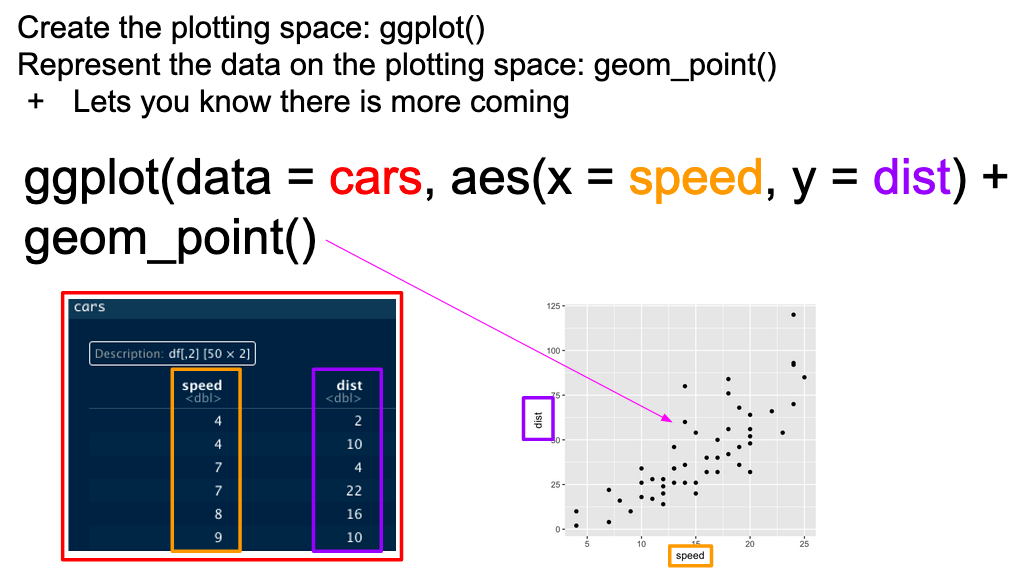
\includegraphics{img/GGplot syntax.png}
\caption{Basic ggplot mappings. Color boxes indicate where the elements go in the function and in the plot.}
\end{figure}

\hypertarget{your-first-ggplot}{%
\section{\texorpdfstring{Your first \texttt{ggplot()}}{Your first ggplot()}}\label{your-first-ggplot}}

Our cider data is already relatively tidy and is much easier to visually inspect, so we will be primarily using it in this section.

Let's begin by making an example \texttt{ggplot()} to demonstrate how it works.

\begin{Shaded}
\begin{Highlighting}[]
\CommentTok{\# We start with our data and pipe it into ggplot}
\NormalTok{raw\_cider\_data }\SpecialCharTok{\%\textgreater{}\%}
  \CommentTok{\# Here we set up the base plot}
  \FunctionTok{ggplot}\NormalTok{(}\AttributeTok{mapping =} \FunctionTok{aes}\NormalTok{(}\AttributeTok{x =}\NormalTok{ MerlynScale\_Ranking, }\AttributeTok{y =}\NormalTok{ Liking)) }\SpecialCharTok{+} 
   \CommentTok{\# Here we tell our base plot to add points}
  \FunctionTok{geom\_point}\NormalTok{()                          }
\end{Highlighting}
\end{Shaded}

\begin{center}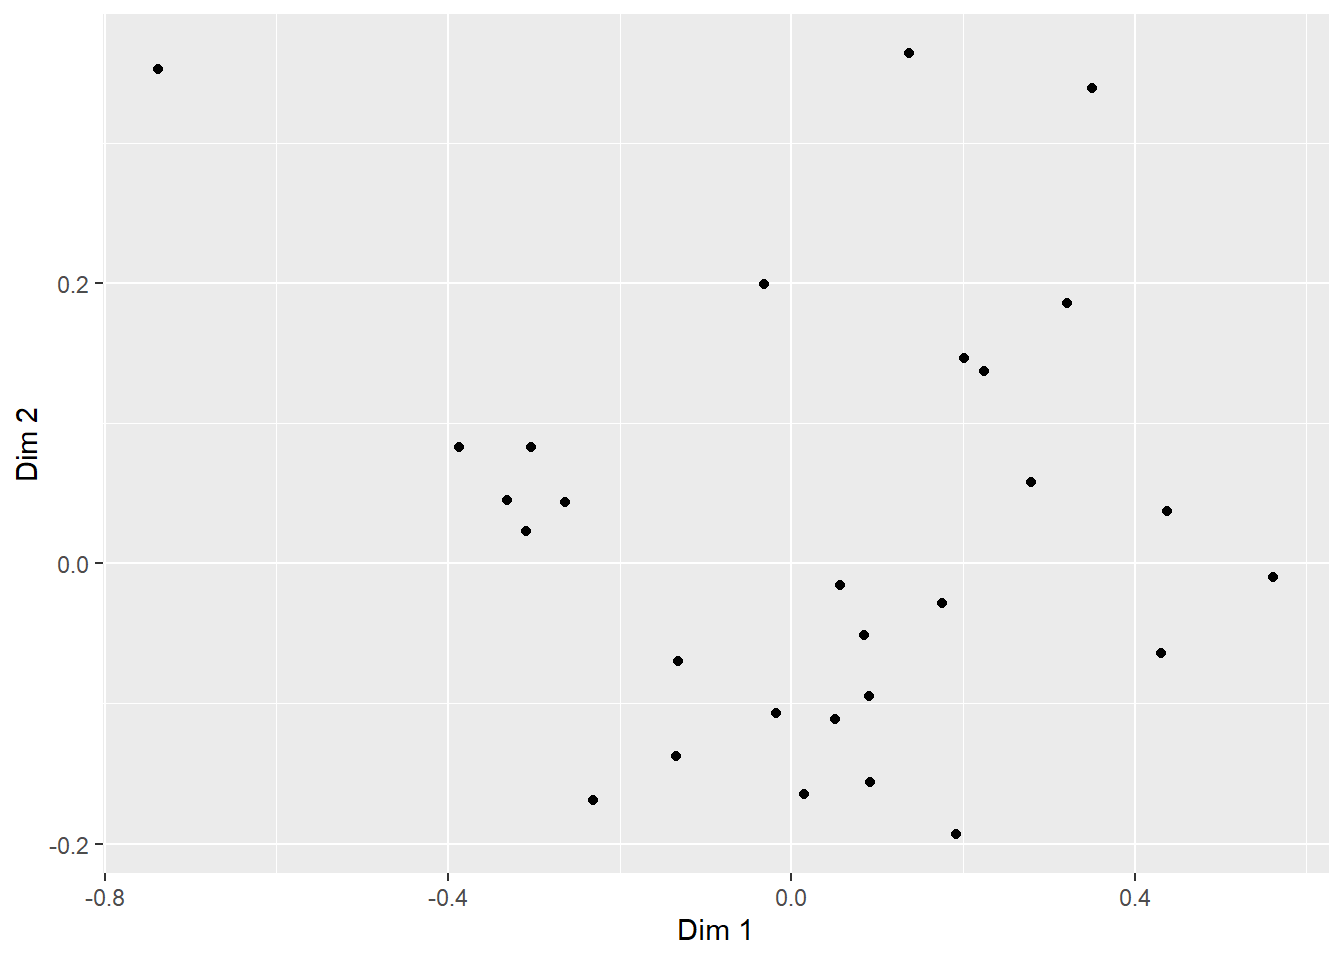
\includegraphics{03-ggplot2-basics_files/figure-latex/a first ggplot-1} \end{center}

This doesn't look all that impressive--partly because the data being plotted itself isn't that sensible, and partly because we haven't made many changes. But before we start looking into that, let's break down the parts of this command.

\hypertarget{the-aes-function-and-mapping-argument}{%
\section{\texorpdfstring{The \texttt{aes()} function and \texttt{mapping\ =} argument}{The aes() function and mapping = argument}}\label{the-aes-function-and-mapping-argument}}

The \texttt{ggplot()} function takes two arguments that are essential, as well as some others you'll rarely use. The first, \texttt{data\ =}, is straightforward, and you'll usually be passing data to the function at the end of some pipeline using \texttt{\%\textgreater{}\%}

The second, \texttt{mapping\ =}, is less clear. This argument requires the \texttt{aes()} function, which can be read as the ``aesthetic'' function. The way that this function works is quite complex, and really not worth digging into here, but I understand it in my head as \textbf{telling \texttt{ggplot()} what part of my data is going to connect to what part of the plot}. So, if we write \texttt{aes(x\ =\ MerlynScale\_Ranking)}, we can read this in our heads as ``the values of x will be mapped from the `MerlynScale\_Ranking' column''.

This sentence tells us the other important thing about \texttt{ggplot()} and the \texttt{aes()} mappings: \textbf{mapped variables each have to be in their own column}. This is another reason that \texttt{ggplot()} requires tidy data.

\hypertarget{adding-layers-with-geom_-functions}{%
\section{\texorpdfstring{Adding layers with \texttt{geom\_*()} functions}{Adding layers with geom\_*() functions}}\label{adding-layers-with-geom_-functions}}

In the above example, we added (literally, using \texttt{+}) a function called \texttt{geom\_point()} to the base \texttt{ggplot()} call. This is functionally a ``layer'' of our plot, that tells \texttt{ggplot2} how to actually visualize the elements specified in the \texttt{aes()} function--in the case of \texttt{geom\_point()}, we create a point for each row's combination of \texttt{x\ =\ MerlynScale\_Ranking} and \texttt{y\ =\ Liking}.

\begin{Shaded}
\begin{Highlighting}[]
\NormalTok{raw\_cider\_data }\SpecialCharTok{\%\textgreater{}\%}
  \FunctionTok{select}\NormalTok{(MerlynScale\_Ranking, Liking)}
\end{Highlighting}
\end{Shaded}

\begin{verbatim}
## # A tibble: 288 x 2
##    MerlynScale_Ranking Liking
##                  <dbl>  <dbl>
##  1                 2.3      6
##  2                 3.5      7
##  3                 2.8      4
##  4                 4.2      2
##  5                 2        7
##  6                 4        5
##  7                 3        8
##  8                 3.3      6
##  9                 3.5      7
## 10                 4.5      3
## # i 278 more rows
\end{verbatim}

There are many \texttt{geom\_*()} functions in \texttt{ggplot2}, and many others defined in other accessory packages. These are the heart of visualizations. We can swap them out to get different results:

\begin{Shaded}
\begin{Highlighting}[]
\NormalTok{raw\_cider\_data }\SpecialCharTok{\%\textgreater{}\%}
  \FunctionTok{ggplot}\NormalTok{(}\AttributeTok{mapping =} \FunctionTok{aes}\NormalTok{(}\AttributeTok{x =}\NormalTok{ MerlynScale\_Ranking, }\AttributeTok{y =}\NormalTok{ Liking)) }\SpecialCharTok{+} 
  \FunctionTok{geom\_smooth}\NormalTok{()}
\end{Highlighting}
\end{Shaded}

\begin{verbatim}
## `geom_smooth()` using method = 'loess' and formula = 'y ~ x'
\end{verbatim}

\begin{center}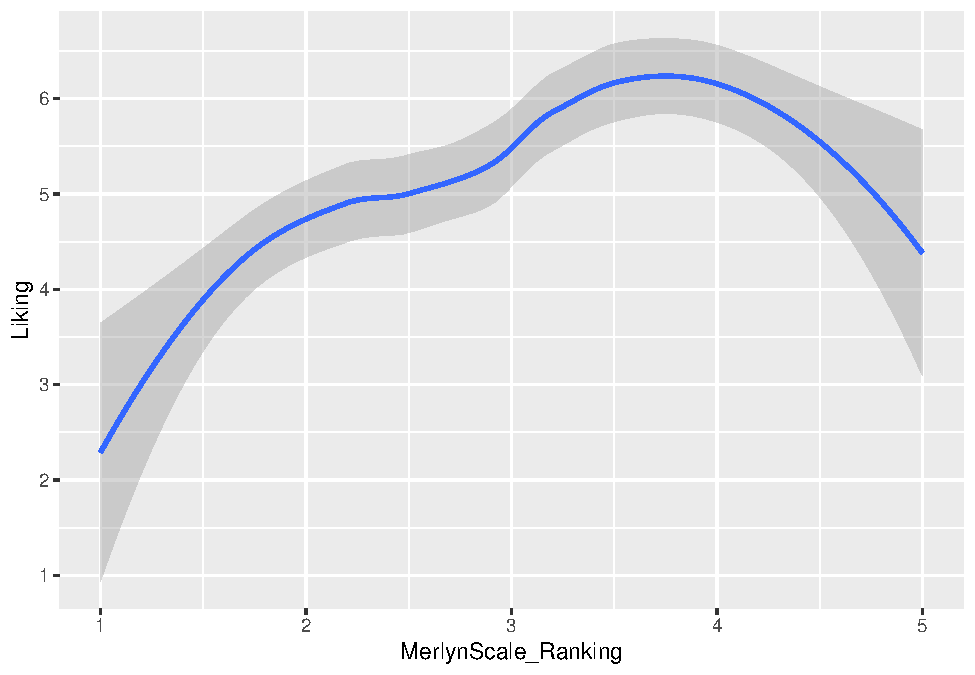
\includegraphics{03-ggplot2-basics_files/figure-latex/switching geom switches the way the data map-1} \end{center}

Here we fit a smoothed line to our data using the default methods in \texttt{geom\_smooth()} (which in this case heuristically defaults to a spline model with LOESS smoothing, but could be linear, GAM, etc).

We can also combine layers, as the term ``layer'' implies:

\begin{Shaded}
\begin{Highlighting}[]
\NormalTok{raw\_cider\_data }\SpecialCharTok{\%\textgreater{}\%}
  \FunctionTok{ggplot}\NormalTok{(}\AttributeTok{mapping =} \FunctionTok{aes}\NormalTok{(}\AttributeTok{x =}\NormalTok{ MerlynScale\_Ranking, }\AttributeTok{y =}\NormalTok{ Liking)) }\SpecialCharTok{+} 
  \FunctionTok{geom\_jitter}\NormalTok{() }\SpecialCharTok{+} \CommentTok{\# add some random noise to show overlapping points}
  \FunctionTok{geom\_smooth}\NormalTok{()}
\end{Highlighting}
\end{Shaded}

\begin{verbatim}
## `geom_smooth()` using method = 'loess' and formula = 'y ~ x'
\end{verbatim}

\begin{center}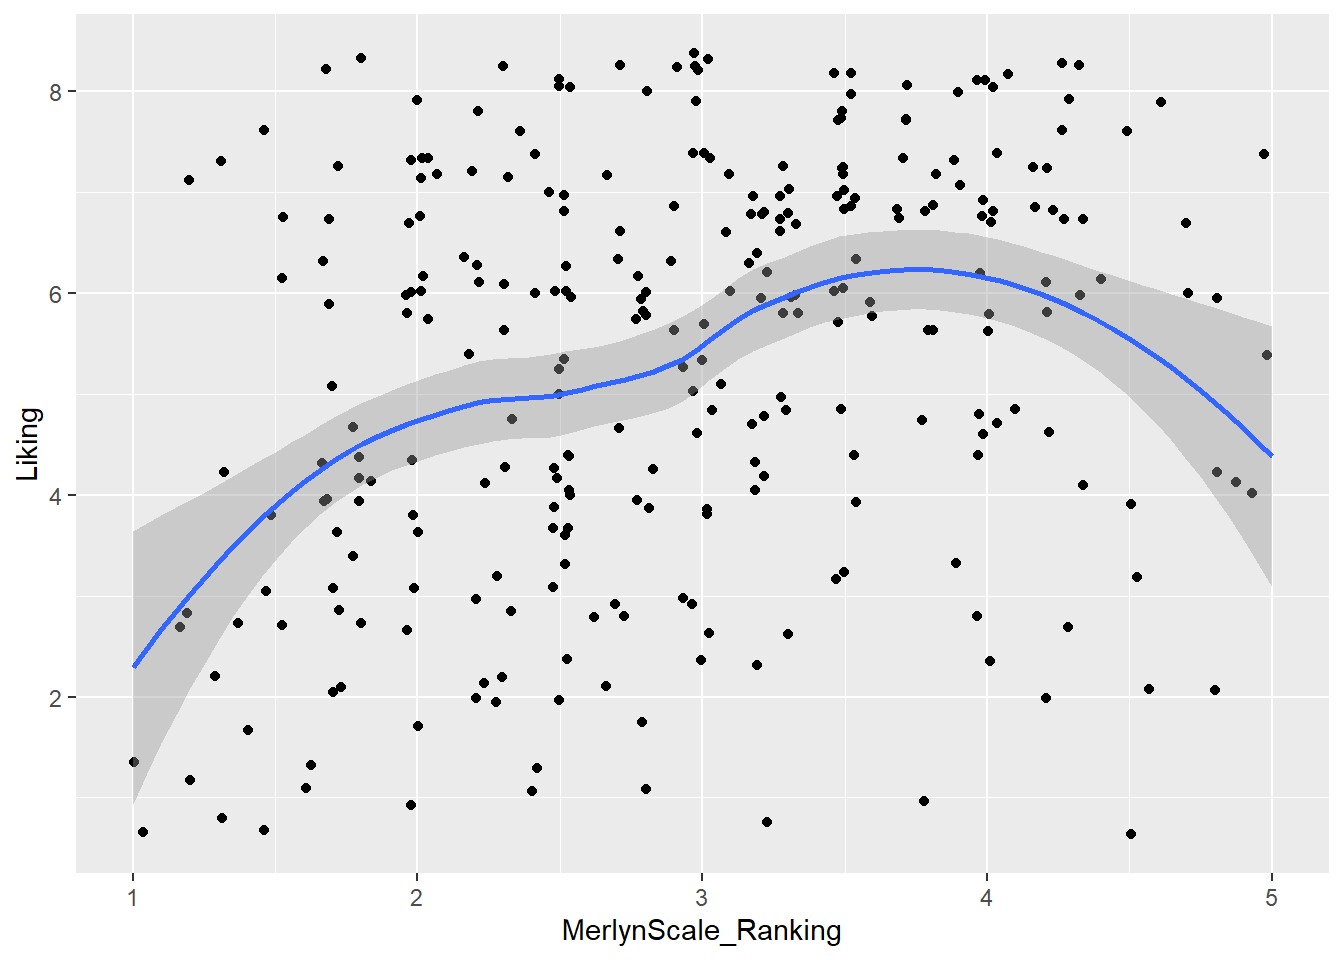
\includegraphics{03-ggplot2-basics_files/figure-latex/geoms are layers in a plot-1} \end{center}

Note that we don't need to tell \emph{either} \texttt{geom\_smooth()} or \texttt{geom\_jitter()} what \texttt{x} and \texttt{y} are--they ``inherit'' them from the \texttt{ggplot()} function to which they are added (\texttt{+}), which defines the plot itself.

What other arguments can be set to aesthetics? Well, we can set other visual properties like \textbf{color}, \textbf{size}, \textbf{transparency} (called ``alpha''), and so on. For example, let's try to look at whether there is a relationship between whether a cider is perceived as ``Dry'' through CATA, measured as ``Dry'' (low values) on the Merlyn Scale, and overall liking.

\begin{Shaded}
\begin{Highlighting}[]
\NormalTok{raw\_cider\_data }\SpecialCharTok{\%\textgreater{}\%}
  \FunctionTok{mutate}\NormalTok{(}\AttributeTok{Dry =} \FunctionTok{as.factor}\NormalTok{(Dry)) }\SpecialCharTok{\%\textgreater{}\%}
  \FunctionTok{ggplot}\NormalTok{(}\AttributeTok{mapping =} \FunctionTok{aes}\NormalTok{(}\AttributeTok{x =}\NormalTok{ MerlynScale\_Ranking, }\AttributeTok{y =}\NormalTok{ Liking, }\AttributeTok{color =}\NormalTok{ Dry)) }\SpecialCharTok{+}
  \FunctionTok{geom\_jitter}\NormalTok{(}\AttributeTok{alpha =} \DecValTok{1}\SpecialCharTok{/}\DecValTok{2}\NormalTok{) }\SpecialCharTok{+} 
  \FunctionTok{scale\_color\_manual}\NormalTok{(}\AttributeTok{values =} \FunctionTok{c}\NormalTok{(}\StringTok{"darkblue"}\NormalTok{, }\StringTok{"darkorange"}\NormalTok{)) }\SpecialCharTok{+} 
  \FunctionTok{theme\_bw}\NormalTok{()}
\end{Highlighting}
\end{Shaded}

\begin{center}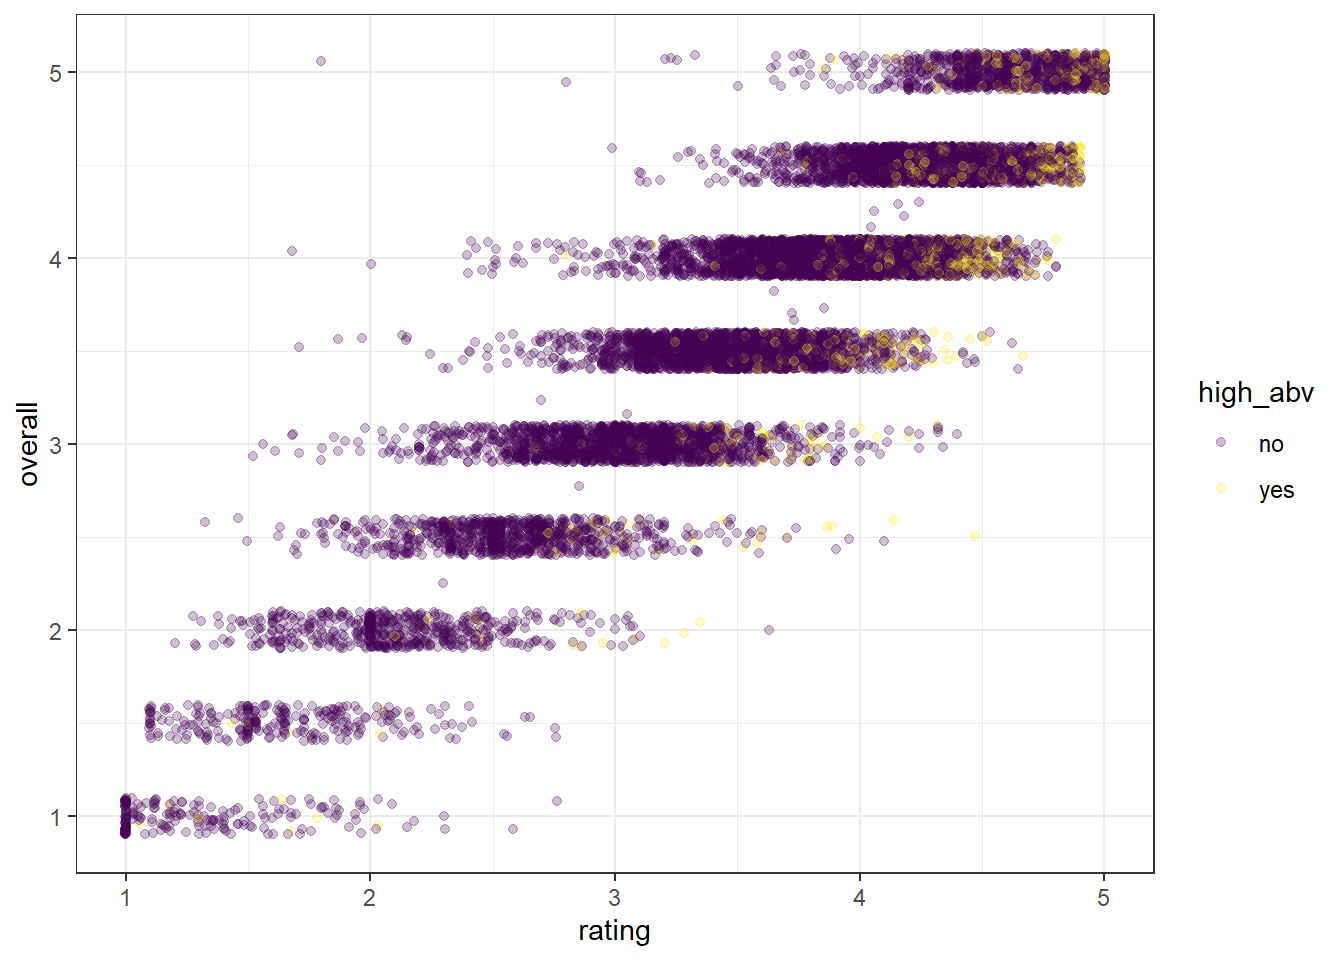
\includegraphics{03-ggplot2-basics_files/figure-latex/here are some other parts of the plot we can control with data-1} \end{center}

We can see that most of the orange dots are to the left side of the figure (associated with lower Merlyn scale ratings), and that most of th3e blue dots are to the right (associated with higher Merlyn Scale ratings). It's hard to make sense of patterns of liking in this visualization, but it looks like ``Dry'' CATA checks may have somewhat lower liking ratings overall.

\hypertarget{arguments-inside-and-outside-of-aes}{%
\section{\texorpdfstring{Arguments inside and outside of \texttt{aes()}}{Arguments inside and outside of aes()}}\label{arguments-inside-and-outside-of-aes}}

In the last plot, we saw an example in the \texttt{geom\_jitter(alpha\ =\ 1/2)} function of setting the \texttt{alpha} (transparency) aesthetic element directly, without using \texttt{aes()} to \textbf{map} a variable to this aesthetic. That is why this is not wrapped in the \texttt{aes()} function. In \texttt{ggplot2}, this is how we set aesthetics to fixed values.

If we had a value we wanted to map transparency to, we would set \texttt{aes(alpha\ =\ \textless{}variable\textgreater{})}. In this dataset, I can't think of a good option for alpha, but note that we can set any variable in these two ways:

\begin{Shaded}
\begin{Highlighting}[]
\CommentTok{\# First, here is the previous figure, showing how we can set aesthetics}
\NormalTok{raw\_cider\_data }\SpecialCharTok{\%\textgreater{}\%}
  \FunctionTok{mutate}\NormalTok{(}\AttributeTok{Dry =} \FunctionTok{as.factor}\NormalTok{(Dry)) }\SpecialCharTok{\%\textgreater{}\%}
  \FunctionTok{ggplot}\NormalTok{(}\FunctionTok{aes}\NormalTok{(}\AttributeTok{x =}\NormalTok{ MerlynScale\_Ranking, }\AttributeTok{y =}\NormalTok{ Liking)) }\SpecialCharTok{+} 
  \CommentTok{\# We can set new aes() mappings in individual layers, as well as the plot itself}
  \FunctionTok{geom\_jitter}\NormalTok{(}\FunctionTok{aes}\NormalTok{(}\AttributeTok{color =}\NormalTok{ Dry)) }\SpecialCharTok{+} 
  \FunctionTok{scale\_color\_manual}\NormalTok{(}\AttributeTok{values =} \FunctionTok{c}\NormalTok{(}\StringTok{"darkblue"}\NormalTok{, }\StringTok{"darkorange"}\NormalTok{)) }\SpecialCharTok{+}
  \FunctionTok{theme\_bw}\NormalTok{()}
\end{Highlighting}
\end{Shaded}

\begin{center}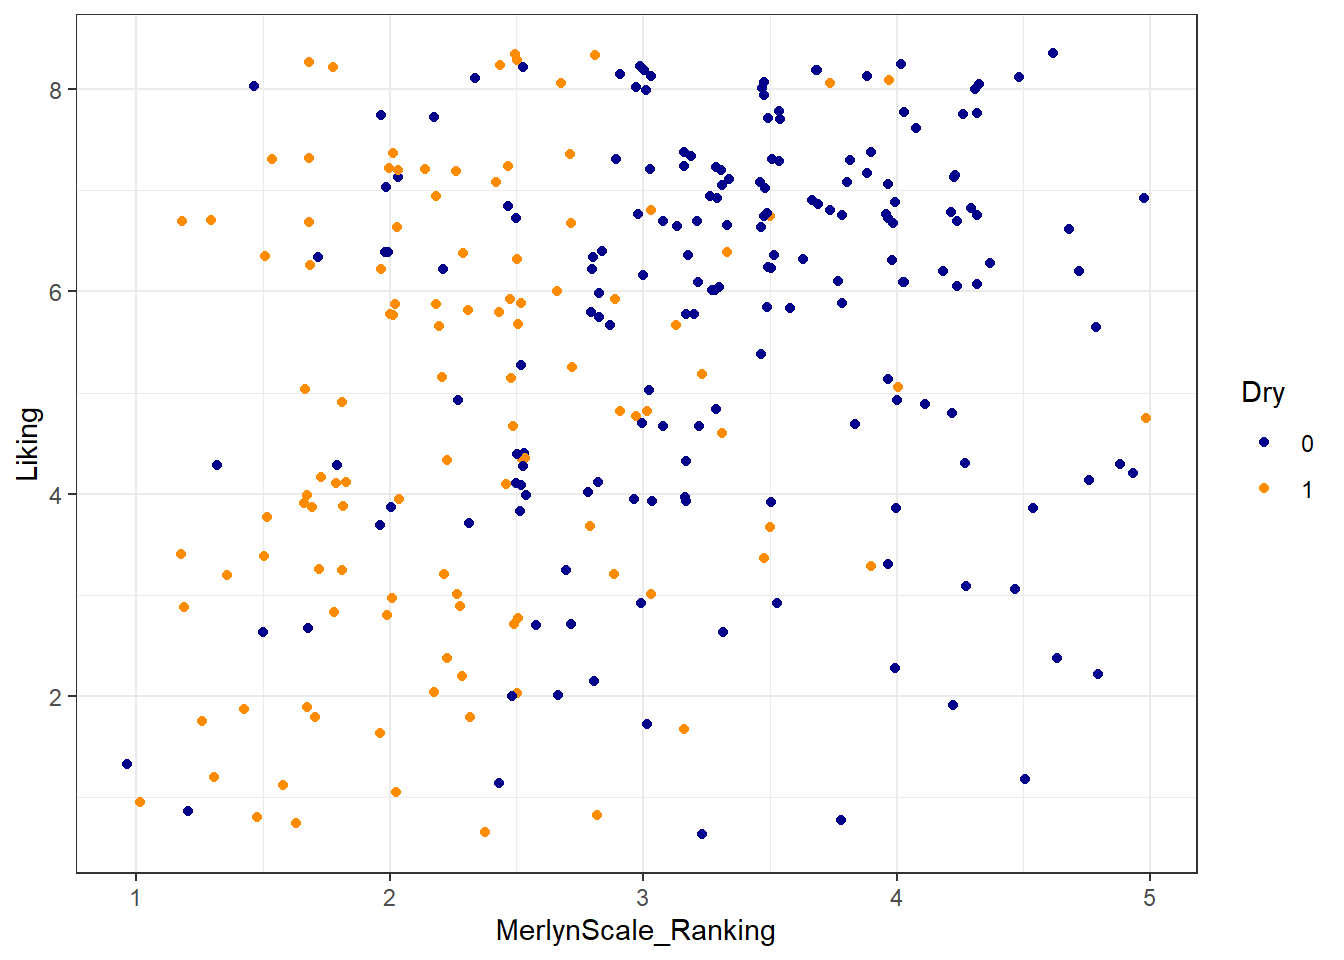
\includegraphics{03-ggplot2-basics_files/figure-latex/using the aes function-1} \end{center}

\begin{Shaded}
\begin{Highlighting}[]
\CommentTok{\# And now we manually set a color for our points: note this means our color}
\CommentTok{\# WON\textquotesingle{}T change with different values of a variable.}
\NormalTok{raw\_cider\_data }\SpecialCharTok{\%\textgreater{}\%}
  \FunctionTok{mutate}\NormalTok{(}\AttributeTok{Dry =} \FunctionTok{as.factor}\NormalTok{(Dry)) }\SpecialCharTok{\%\textgreater{}\%}
  \FunctionTok{ggplot}\NormalTok{(}\FunctionTok{aes}\NormalTok{(}\AttributeTok{x =}\NormalTok{ MerlynScale\_Ranking, }\AttributeTok{y =}\NormalTok{ Liking)) }\SpecialCharTok{+} 
  \CommentTok{\# notice we no longer use aes() below, and color no longer matches \textasciigrave{}Dry\textasciigrave{}}
  \FunctionTok{geom\_jitter}\NormalTok{(}\AttributeTok{color =} \StringTok{"darkorange"}\NormalTok{) }\SpecialCharTok{+} 
  \FunctionTok{theme\_bw}\NormalTok{()}
\end{Highlighting}
\end{Shaded}

\begin{center}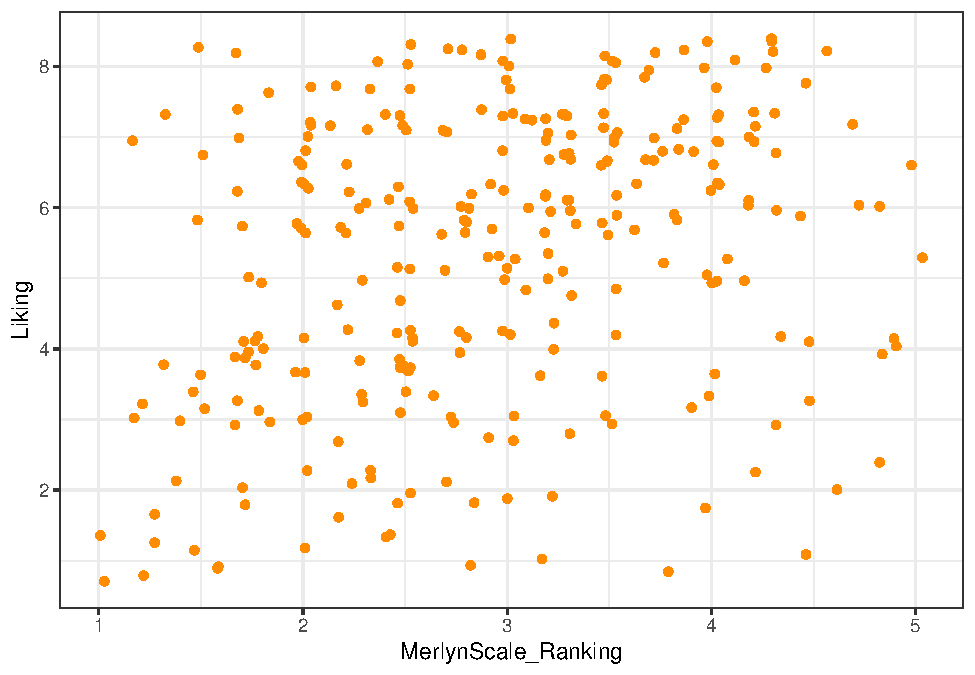
\includegraphics{03-ggplot2-basics_files/figure-latex/using the aes function-2} \end{center}

\hypertarget{using-theme_-to-change-visual-options-quickly}{%
\subsection{\texorpdfstring{Using \texttt{theme\_*()} to change visual options quickly}{Using theme\_*() to change visual options quickly}}\label{using-theme_-to-change-visual-options-quickly}}

In the last several plots, notice that we have changed from the default (and to my mind unattractive) grey background of \texttt{ggplot2} to a black and white theme. This is by adding a \texttt{theme\_bw()} call to the list of commands. \texttt{ggplot2} includes a number of default \texttt{theme\_*()} functions, and you can get many more through other \texttt{R} packages. They can have subtle to dramatic effects:

\begin{Shaded}
\begin{Highlighting}[]
\NormalTok{raw\_cider\_data }\SpecialCharTok{\%\textgreater{}\%}
  \FunctionTok{ggplot}\NormalTok{(}\FunctionTok{aes}\NormalTok{(}\AttributeTok{x =}\NormalTok{ MerlynScale\_Ranking, }\AttributeTok{y =}\NormalTok{ Liking)) }\SpecialCharTok{+} 
  \FunctionTok{geom\_jitter}\NormalTok{() }\SpecialCharTok{+} 
  \FunctionTok{theme\_void}\NormalTok{()}
\end{Highlighting}
\end{Shaded}

\begin{center}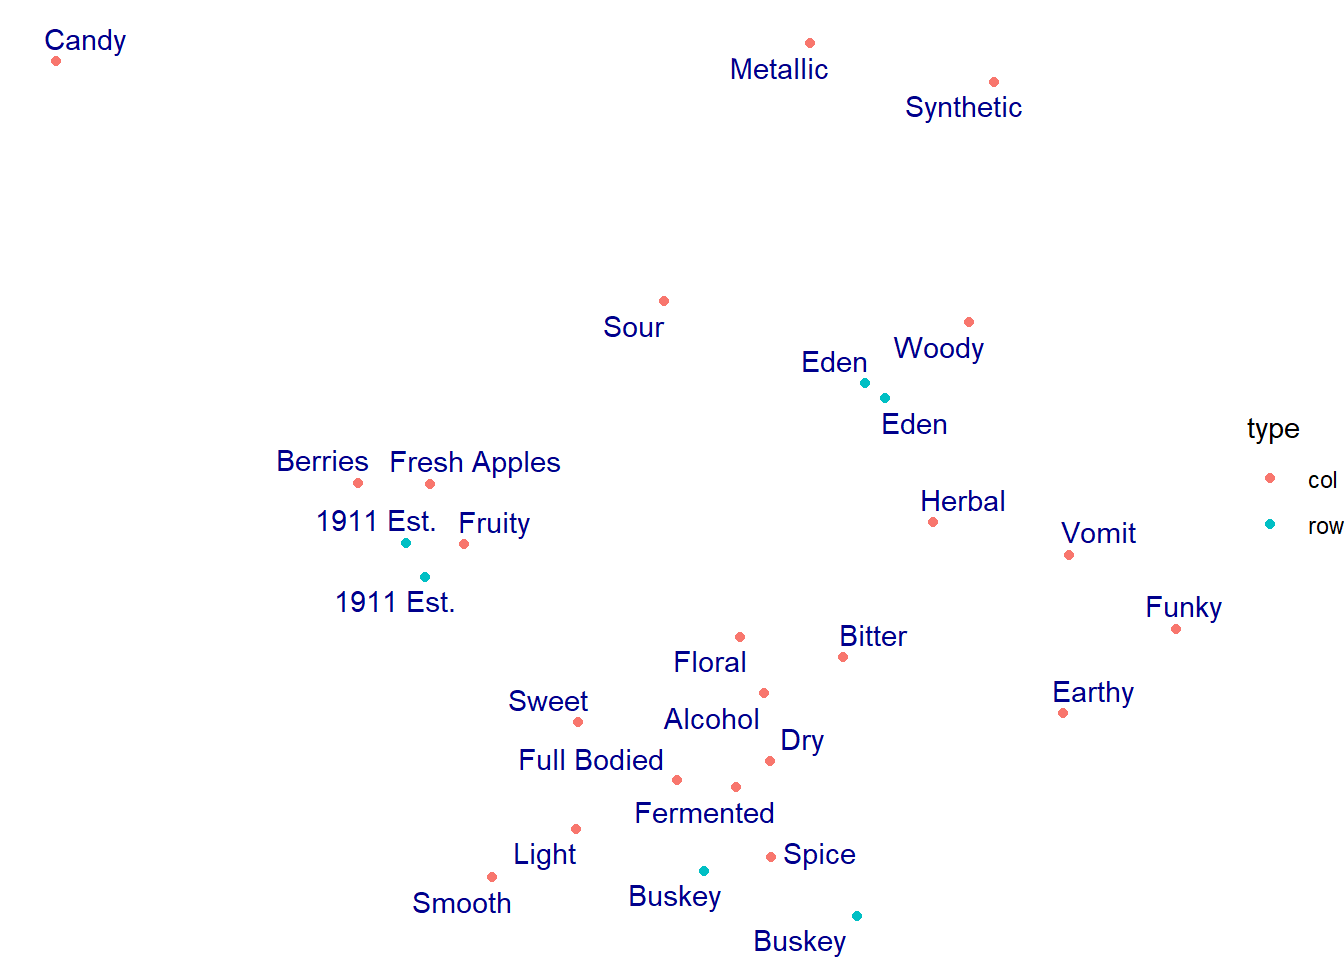
\includegraphics{03-ggplot2-basics_files/figure-latex/using the theme functions-1} \end{center}

You can edit every last element of the plot's theme using the base \texttt{theme()} function, which is powerful but a little bit tricky to use.

\begin{Shaded}
\begin{Highlighting}[]
\NormalTok{raw\_cider\_data }\SpecialCharTok{\%\textgreater{}\%}
  \FunctionTok{ggplot}\NormalTok{(}\FunctionTok{aes}\NormalTok{(}\AttributeTok{x =}\NormalTok{ MerlynScale\_Ranking, }\AttributeTok{y =}\NormalTok{ Liking)) }\SpecialCharTok{+} 
  \FunctionTok{geom\_jitter}\NormalTok{() }\SpecialCharTok{+} 
  \FunctionTok{theme\_bw}\NormalTok{() }\SpecialCharTok{+} 
  \CommentTok{\# we use theme() to remove grid lines, for example}
  \FunctionTok{theme}\NormalTok{(}\AttributeTok{panel.grid =} \FunctionTok{element\_blank}\NormalTok{())}
\end{Highlighting}
\end{Shaded}

\begin{center}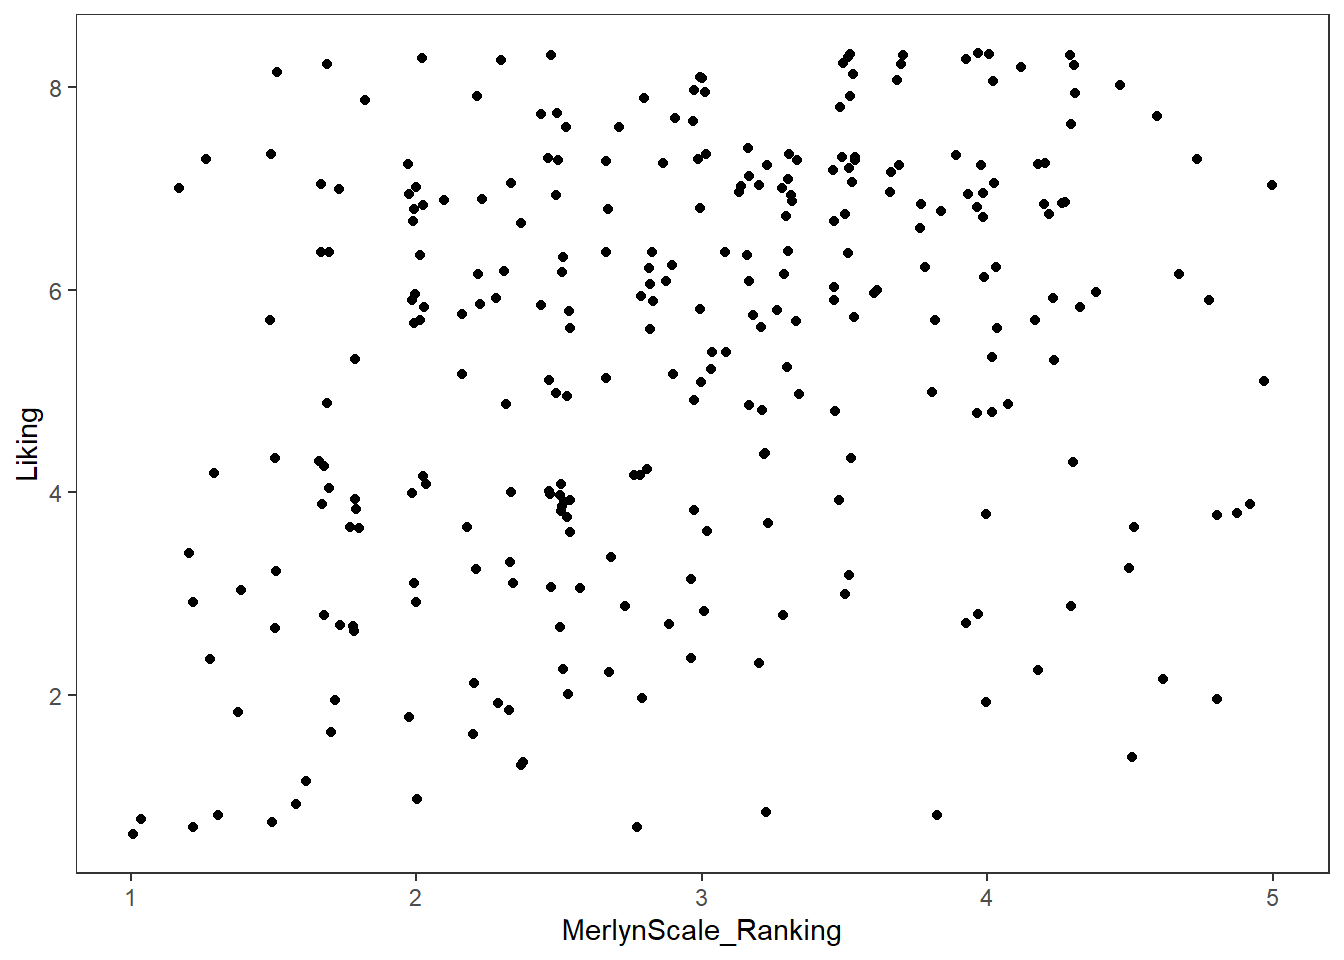
\includegraphics{03-ggplot2-basics_files/figure-latex/using theme-1} \end{center}

Most of the use of \texttt{theme()} involves functions names as \texttt{element\_*()}. When we remove elements, for example, we use \texttt{element\_blank()} (not, for example, \texttt{NA} or \texttt{NULL} as we typically would in other parts of \texttt{R}).

Finally, we can set default themes for a particular script using the \texttt{theme\_set()} function. We can also use this to set custom defaults:

\begin{Shaded}
\begin{Highlighting}[]
\FunctionTok{theme\_set}\NormalTok{(}
  \FunctionTok{theme\_bw}\NormalTok{() }\SpecialCharTok{+} 
    \FunctionTok{theme}\NormalTok{(}\AttributeTok{panel.grid.minor =} \FunctionTok{element\_blank}\NormalTok{())}
\NormalTok{)}

\NormalTok{raw\_cider\_data }\SpecialCharTok{\%\textgreater{}\%}
  \FunctionTok{ggplot}\NormalTok{(}\FunctionTok{aes}\NormalTok{(}\AttributeTok{x =}\NormalTok{ MerlynScale\_Ranking, }\AttributeTok{y =}\NormalTok{ Liking)) }\SpecialCharTok{+} 
  \FunctionTok{geom\_jitter}\NormalTok{()}
\end{Highlighting}
\end{Shaded}

\begin{center}\includegraphics{03-ggplot2-basics_files/figure-latex/unnamed-chunk-1-1} \end{center}

All plots from here on will \emph{default} to the \texttt{theme\_bw()} theme, with the ``minor'' grid lines removed for a cleaner grid look.

\hypertarget{changing-aesthetic-elements-with-scale_-functions}{%
\subsection{\texorpdfstring{Changing aesthetic elements with \texttt{scale\_*()} functions}{Changing aesthetic elements with scale\_*() functions}}\label{changing-aesthetic-elements-with-scale_-functions}}

Finally, say we didn't like the default color set for the points.

How can we manipulate the colors that are plotted? The \textbf{way in which} mapped, aesthetic variables are assigned to visual elements is controlled by the \texttt{scale\_*()} functions.

In my experience, the most frequently encountered scales are those for color: either \texttt{scale\_fill\_*()} for solid objects (like the bars in a histogram) or \texttt{scale\_color\_*()} for lines and points (like the outlines of the histogram bars).

Scale functions work by telling \texttt{ggplot()} \emph{how} to map aesthetic variables to visual elements. You may have noticed that I added a \texttt{scale\_color\_manual()} function to the end of several plots above. This function lets me manually specify the colors that are assigned to each colored element.

\begin{Shaded}
\begin{Highlighting}[]
\NormalTok{p }\OtherTok{\textless{}{-}} 
\NormalTok{  raw\_cider\_data }\SpecialCharTok{\%\textgreater{}\%}
  \FunctionTok{mutate}\NormalTok{(}\AttributeTok{Dry =} \FunctionTok{as.factor}\NormalTok{(Dry)) }\SpecialCharTok{\%\textgreater{}\%}
  \CommentTok{\# This block gets us a subset of beer styles for clear visualization}
  \FunctionTok{ggplot}\NormalTok{(}\AttributeTok{mapping =} \FunctionTok{aes}\NormalTok{(}\AttributeTok{x =}\NormalTok{ Liking)) }\SpecialCharTok{+} 
  \FunctionTok{geom\_density}\NormalTok{(}\AttributeTok{mapping =} \FunctionTok{aes}\NormalTok{(}\AttributeTok{fill =}\NormalTok{ Dry), }\AttributeTok{alpha =} \DecValTok{1}\SpecialCharTok{/}\DecValTok{3}\NormalTok{, }\AttributeTok{color =} \StringTok{"transparent"}\NormalTok{)}

\NormalTok{p}
\end{Highlighting}
\end{Shaded}

\begin{center}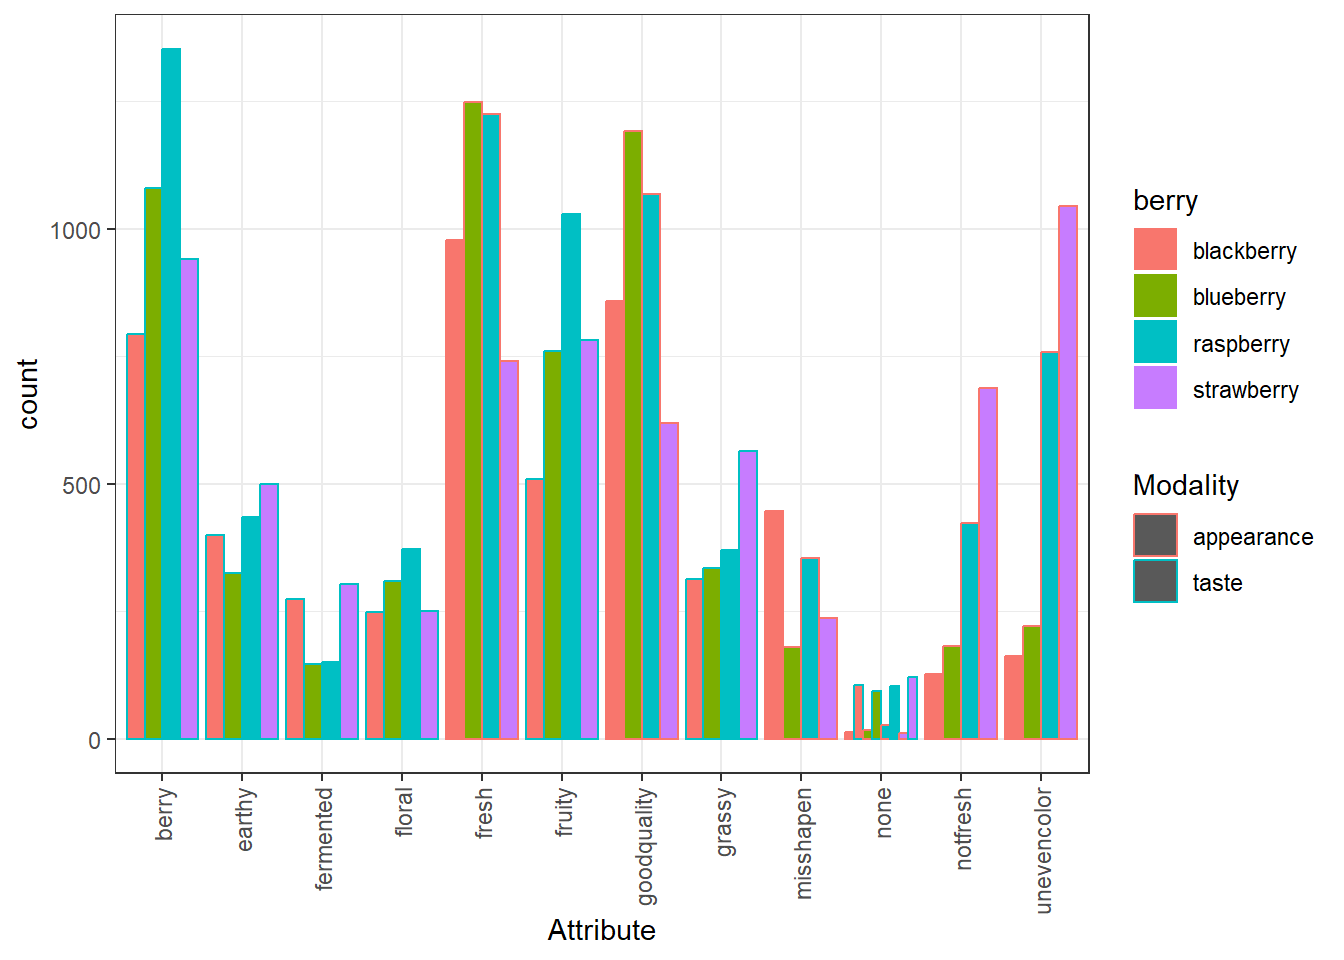
\includegraphics{03-ggplot2-basics_files/figure-latex/ggplots are R objects-1} \end{center}

We can take a saved plot (like \texttt{p}) and use scales to change how it is visualized.

\begin{Shaded}
\begin{Highlighting}[]
\NormalTok{p }\SpecialCharTok{+} \FunctionTok{scale\_fill\_viridis\_d}\NormalTok{()}
\end{Highlighting}
\end{Shaded}

\begin{center}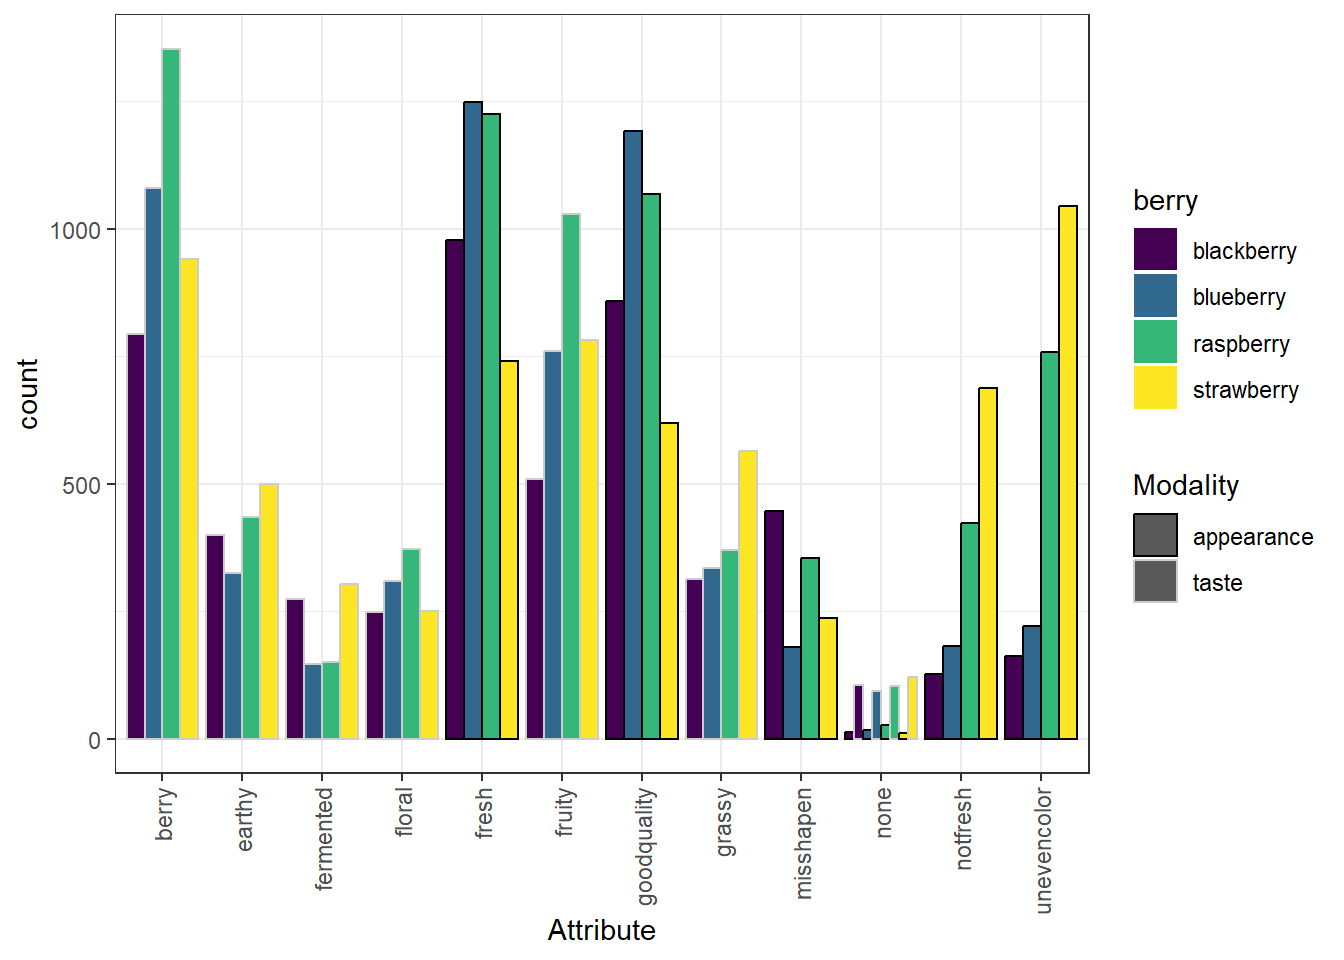
\includegraphics{03-ggplot2-basics_files/figure-latex/we can modify stored plots after the fact-1} \end{center}

\texttt{ggplot2} has a broad range of built-in options for scales, but there are many others available in add-on packages that build on top of it. The \texttt{scale\_*\_viridis\_*()} functions use a package callled \texttt{viridis} that provides (theoretically) color-blind safe colors for both continuous (gradient) and categorical (discrete) mappings, but I do find that their defaults (using light colors like yellow on one end of the scale) are hard to see for anyone!

As we saw above, you can also build your own scales using the \texttt{scale\_*\_manual()} functions, in which you give a vector of the same length as your mapped aesthetic variable in order to set up the visual assignment. That sounds jargon-y, so here is an example:

\begin{Shaded}
\begin{Highlighting}[]
\CommentTok{\# We\textquotesingle{}ll pick 14 random colors from the colors R knows about}
\NormalTok{random\_colors }\OtherTok{\textless{}{-}} \FunctionTok{print}\NormalTok{(}\FunctionTok{colors}\NormalTok{()[}\FunctionTok{sample}\NormalTok{(}\AttributeTok{x =} \DecValTok{1}\SpecialCharTok{:}\FunctionTok{length}\NormalTok{(}\FunctionTok{colors}\NormalTok{()), }\AttributeTok{size =} \DecValTok{10}\NormalTok{)])}
\end{Highlighting}
\end{Shaded}

\begin{verbatim}
##  [1] "goldenrod3"      "honeydew4"       "green"           "indianred2"     
##  [5] "orange4"         "paleturquoise2"  "lightsteelblue2" "lightgoldenrod" 
##  [9] "grey76"          "khaki"
\end{verbatim}

\begin{Shaded}
\begin{Highlighting}[]
\NormalTok{p }\SpecialCharTok{+} 
  \FunctionTok{scale\_fill\_manual}\NormalTok{(}\AttributeTok{values =}\NormalTok{ random\_colors)}
\end{Highlighting}
\end{Shaded}

\begin{center}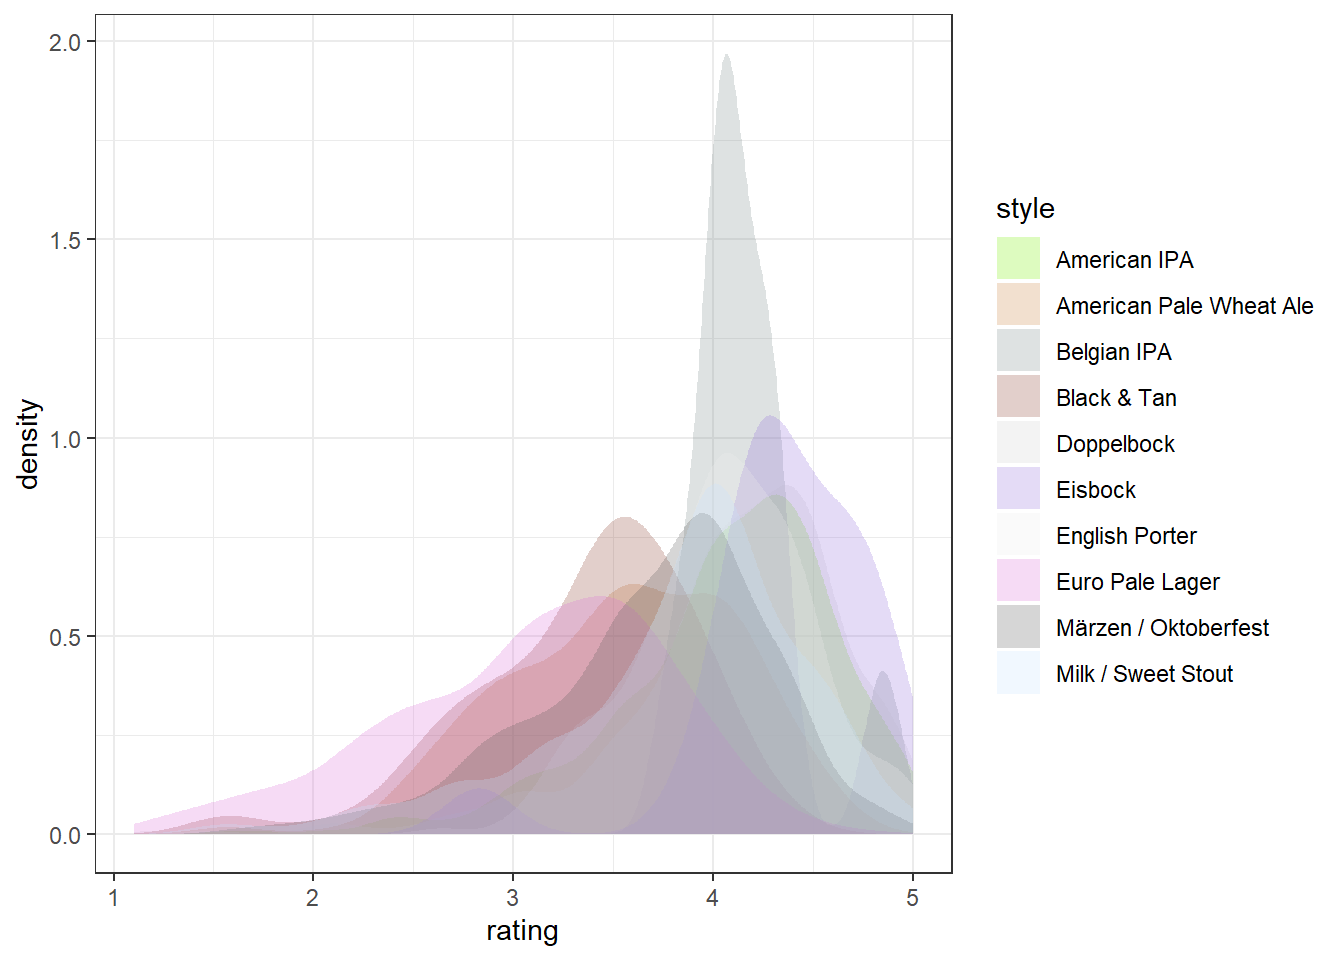
\includegraphics{03-ggplot2-basics_files/figure-latex/another example of posthoc plot modification-1} \end{center}

\hypertarget{finally-facet_}{%
\subsection{\texorpdfstring{Finally, \texttt{facet\_*()}}{Finally, facet\_*()}}\label{finally-facet_}}

The last powerful tool I want to show off is the ability of \texttt{ggplot2} to make what\href{https://socviz.co/groupfacettx.html\#facet-to-make-small-multiples}{Edward Tufte called ``small multiples''}: breaking out the data into multiple, identical plots by some categorical classifier in order to show trends more effectively.

So far we've seen how to visualize the overall liking of ciders in our small data set by the Merlyn Scale Ranking, and how to assign color, transparency, and fill to other attributes. We can use such an approach to get a quick picture of the CATA selections for each cider in a clear, easy to see visualization:

\begin{Shaded}
\begin{Highlighting}[]
\NormalTok{raw\_cider\_data }\SpecialCharTok{\%\textgreater{}\%}
  \FunctionTok{pivot\_longer}\NormalTok{(Fresh\_Apples}\SpecialCharTok{:}\NormalTok{Synthetic) }\SpecialCharTok{\%\textgreater{}\%}
  \FunctionTok{group\_by}\NormalTok{(Sample\_Name, Temperature, name) }\SpecialCharTok{\%\textgreater{}\%}
  \FunctionTok{summarize}\NormalTok{(}\AttributeTok{total =} \FunctionTok{sum}\NormalTok{(value)) }\SpecialCharTok{\%\textgreater{}\%}
  \FunctionTok{ggplot}\NormalTok{(}\FunctionTok{aes}\NormalTok{(}\AttributeTok{x =} \FunctionTok{interaction}\NormalTok{(Sample\_Name, Temperature), }\AttributeTok{y =}\NormalTok{ total)) }\SpecialCharTok{+} 
  \FunctionTok{geom\_col}\NormalTok{(}\FunctionTok{aes}\NormalTok{(}\AttributeTok{fill =}\NormalTok{ Sample\_Name)) }\SpecialCharTok{+}
  \FunctionTok{scale\_fill\_manual}\NormalTok{(}\AttributeTok{values =}\NormalTok{ wesanderson}\SpecialCharTok{::}\NormalTok{wes\_palettes}\SpecialCharTok{$}\NormalTok{FantasticFox1) }\SpecialCharTok{+} 
  \FunctionTok{coord\_flip}\NormalTok{() }\SpecialCharTok{+} 
  \FunctionTok{facet\_wrap}\NormalTok{(}\SpecialCharTok{\textasciitilde{}}\NormalTok{name, }\AttributeTok{ncol =} \DecValTok{6}\NormalTok{) }\SpecialCharTok{+} 
  \FunctionTok{labs}\NormalTok{(}\AttributeTok{x =} \ConstantTok{NULL}\NormalTok{, }\AttributeTok{y =} \ConstantTok{NULL}\NormalTok{, }\AttributeTok{fill =} \ConstantTok{NULL}\NormalTok{) }\SpecialCharTok{+} 
  \FunctionTok{theme}\NormalTok{(}\AttributeTok{legend.position =} \StringTok{"top"}\NormalTok{)}
\end{Highlighting}
\end{Shaded}

\begin{verbatim}
## `summarise()` has grouped output by 'Sample_Name', 'Temperature'. You can
## override using the `.groups` argument.
\end{verbatim}

\begin{center}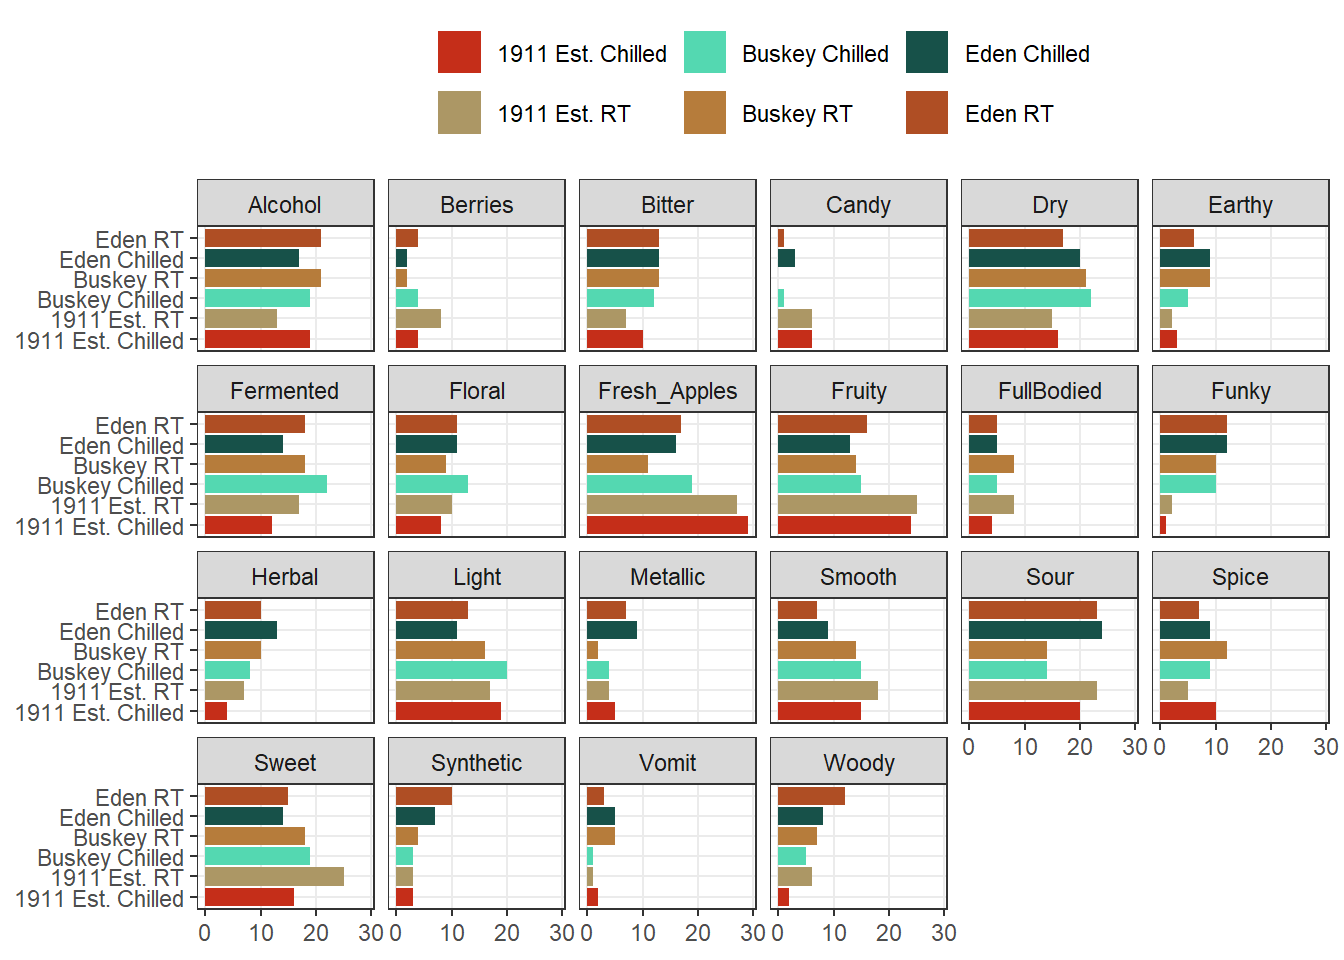
\includegraphics{03-ggplot2-basics_files/figure-latex/cider-facets-1} \end{center}

We can see that overall for the most frequently used attributes, the serving temperature doesn't matter (and for the most part there is some reassuring consistency in the use of terms to describe each cider at different temperatures).

But in the previous part of this workshop, we showed much more complex plots for our berry data, which showed the same plot broken up by a classifying variable: this is called ``faceting''. Let's return from our cider data to our berry data in order to finally complete the workflow I showed in the beginning of the workshop.

Now we are prepared to walk through the entire workflow

\begin{Shaded}
\begin{Highlighting}[]
\CommentTok{\# First we wrangle our data using the tools we\textquotesingle{}ve learned to get penalties/lifts}
\CommentTok{\# for each attributes}
\NormalTok{berry\_penalty\_analysis\_data }\OtherTok{\textless{}{-}} 
\NormalTok{  berry\_long\_cata }\SpecialCharTok{\%\textgreater{}\%}
  \FunctionTok{group\_by}\NormalTok{(berry, cata\_variable, checked) }\SpecialCharTok{\%\textgreater{}\%}
  \FunctionTok{summarize}\NormalTok{(}\AttributeTok{penalty\_lift =} \FunctionTok{mean}\NormalTok{(rating),}
            \AttributeTok{count =} \FunctionTok{n}\NormalTok{()) }\SpecialCharTok{\%\textgreater{}\%}
  \FunctionTok{ungroup}\NormalTok{() }
\end{Highlighting}
\end{Shaded}

\begin{verbatim}
## `summarise()` has grouped output by 'berry', 'cata_variable'. You can override
## using the `.groups` argument.
\end{verbatim}

\begin{Shaded}
\begin{Highlighting}[]
\NormalTok{p1\_berry\_penalty }\OtherTok{\textless{}{-}} 
  
  \CommentTok{\# We start by widening our data just a bit, and use a function to give some}
  \CommentTok{\# better names to our mean values for when an attribute it checked (1) or not}
  \CommentTok{\# (0).}
  
\NormalTok{  berry\_penalty\_analysis\_data }\SpecialCharTok{\%\textgreater{}\%}
  \FunctionTok{select}\NormalTok{(}\SpecialCharTok{{-}}\NormalTok{count) }\SpecialCharTok{\%\textgreater{}\%}
  \FunctionTok{pivot\_wider}\NormalTok{(}\AttributeTok{names\_from =}\NormalTok{ checked,}
              \AttributeTok{values\_from =}\NormalTok{ penalty\_lift,}
              \AttributeTok{names\_prefix =} \StringTok{"checked\_"}\NormalTok{) }\SpecialCharTok{\%\textgreater{}\%}
  
  \CommentTok{\# Then we actually calculate the penalty/lift: what is the difference in the}
  \CommentTok{\# mean liking when an attribute is checked or not?}
  
  \FunctionTok{group\_by}\NormalTok{(berry, cata\_variable) }\SpecialCharTok{\%\textgreater{}\%}
  \FunctionTok{summarize}\NormalTok{(}\AttributeTok{penalty\_lift =}\NormalTok{ checked\_1 }\SpecialCharTok{{-}}\NormalTok{ checked\_0) }\SpecialCharTok{\%\textgreater{}\%}
  
  \CommentTok{\# We have two kinds of CATA attibutes: visual assessment and by{-}mouth}
  \CommentTok{\# assessment.  It would be nice to keep track.}
  
  \FunctionTok{separate}\NormalTok{(cata\_variable, }
           \AttributeTok{into =} \FunctionTok{c}\NormalTok{(}\StringTok{"mode"}\NormalTok{, }\StringTok{"variable"}\NormalTok{), }
           \AttributeTok{sep =} \StringTok{"\_"}\NormalTok{) }\SpecialCharTok{\%\textgreater{}\%}
  
  \CommentTok{\# Fix a typo}
  
  \FunctionTok{mutate}\NormalTok{(}\AttributeTok{mode =} \FunctionTok{str\_replace}\NormalTok{(mode, }\StringTok{"appearane"}\NormalTok{, }\StringTok{"appearance"}\NormalTok{)) }\SpecialCharTok{\%\textgreater{}\%}
  \FunctionTok{mutate}\NormalTok{(}\AttributeTok{mode =} \FunctionTok{case\_when}\NormalTok{(mode }\SpecialCharTok{==} \StringTok{"taste"} \SpecialCharTok{\textasciitilde{}} \StringTok{"(T)"}\NormalTok{,}
\NormalTok{                          mode }\SpecialCharTok{==} \StringTok{"appearance"} \SpecialCharTok{\textasciitilde{}} \StringTok{"(A)"}\NormalTok{)) }\SpecialCharTok{\%\textgreater{}\%}
  \FunctionTok{unite}\NormalTok{(variable, mode, }\AttributeTok{col =} \StringTok{"cata\_variable"}\NormalTok{, }\AttributeTok{sep =} \StringTok{" "}\NormalTok{) }\SpecialCharTok{\%\textgreater{}\%}
  
  \CommentTok{\# We are using a function from tidytext that makes faceting the final figure}
  \CommentTok{\# easier: reorder\_within() makes a set of factors able to be ordered}
  \CommentTok{\# differently within another variable.  In this case, we have different}
  \CommentTok{\# attributes and different penalties within each berry by design}
  
  \FunctionTok{mutate}\NormalTok{(}\AttributeTok{cata\_variable =}\NormalTok{ tidytext}\SpecialCharTok{::}\FunctionTok{reorder\_within}\NormalTok{(}\AttributeTok{x =}\NormalTok{ cata\_variable,}
                                                  \AttributeTok{by =}\NormalTok{ penalty\_lift,}
                                                  \AttributeTok{within =}\NormalTok{ berry)) }\SpecialCharTok{\%\textgreater{}\%}
  
  \CommentTok{\#And finally we plot!}
  
  \FunctionTok{ggplot}\NormalTok{(}\AttributeTok{mapping =} \FunctionTok{aes}\NormalTok{(}\AttributeTok{x =}\NormalTok{ cata\_variable, }\AttributeTok{y =}\NormalTok{ penalty\_lift)) }\SpecialCharTok{+}
  \FunctionTok{geom\_col}\NormalTok{(}\FunctionTok{aes}\NormalTok{(}\AttributeTok{fill =}\NormalTok{ penalty\_lift), }\AttributeTok{color =} \StringTok{"white"}\NormalTok{, }\AttributeTok{show.legend =} \ConstantTok{FALSE}\NormalTok{) }\SpecialCharTok{+} 
  \FunctionTok{facet\_wrap}\NormalTok{(}\SpecialCharTok{\textasciitilde{}}\NormalTok{berry, }\AttributeTok{scales =} \StringTok{"free"}\NormalTok{, }\AttributeTok{nrow =} \DecValTok{1}\NormalTok{) }\SpecialCharTok{+} 
  
  \CommentTok{\# To take advantage of our newly reordered factors, we also need to use the}
  \CommentTok{\# matching tidytext::scale\_x\_reordered() function}
  
\NormalTok{  tidytext}\SpecialCharTok{::}\FunctionTok{scale\_x\_reordered}\NormalTok{() }\SpecialCharTok{+} 
  \FunctionTok{coord\_flip}\NormalTok{() }\SpecialCharTok{+} 
  \FunctionTok{theme\_classic}\NormalTok{() }\SpecialCharTok{+} 
  \FunctionTok{scale\_fill\_gradient}\NormalTok{(}\AttributeTok{low =} \StringTok{"tan"}\NormalTok{, }\AttributeTok{high =} \StringTok{"darkgreen"}\NormalTok{) }\SpecialCharTok{+} 
  \FunctionTok{labs}\NormalTok{(}\AttributeTok{x =} \ConstantTok{NULL}\NormalTok{, }\AttributeTok{y =} \ConstantTok{NULL}\NormalTok{,}
       \AttributeTok{title =} \StringTok{"Penalty / Lift Analysis"}\NormalTok{,}
       \AttributeTok{subtitle =} \StringTok{"displays the mean difference (within berries) for when a CATA variable is checked}\SpecialCharTok{\textbackslash{}n}\StringTok{or un{-}checked"}\NormalTok{)}
\end{Highlighting}
\end{Shaded}

\begin{verbatim}
## `summarise()` has grouped output by 'berry'. You can override using the
## `.groups` argument.
\end{verbatim}

\begin{Shaded}
\begin{Highlighting}[]
\NormalTok{p1\_berry\_penalty}
\end{Highlighting}
\end{Shaded}

\begin{center}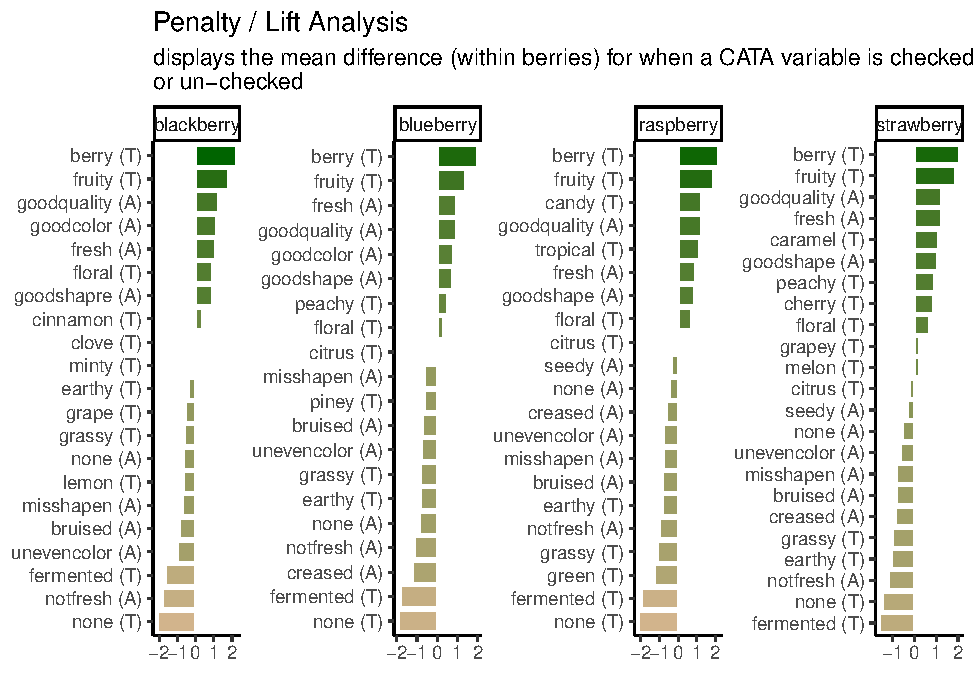
\includegraphics{03-ggplot2-basics_files/figure-latex/berry-penalty-plots-1} \end{center}

We can see that the 2 most important attributes for driving liking are the same across all 4 berries, but that the highest penalty is different across them.

\hypertarget{some-further-reading}{%
\section{Some further reading}\label{some-further-reading}}

This has been a lightning tour of \texttt{ggplot2} as preparatory material for our core material on text analysis; it barely scratches the surface. If you're interested in learning more, I recommend taking a look at the following sources:

\begin{enumerate}
\def\labelenumi{\arabic{enumi}.}
\tightlist
\item
  Kieran Healy's ``\href{https://socviz.co/index.html\#preface}{Data Visualization: a Practical Introduction}''.
\item
  The plotting section of \href{https://r4ds.had.co.nz/data-visualisation.html}{R for Data Science}.
\item
  Hadley Wickham's core reference textbook on \href{https://ggplot2-book.org/}{ggplot2}.
\end{enumerate}

\hypertarget{using-ggplot-with-other-packages}{%
\chapter{Using ggplot with Other Packages}\label{using-ggplot-with-other-packages}}

As you might have noticed, we had you download more packages than just \texttt{ggplot2} for this tutorial. \texttt{ggplot2} is a framework and will help you make many standard plots, but it can't do everything. Or, sometimes, you may not want to use it to do everything yourself.

Packages meant to work with \texttt{ggplot2} to more easily make specific kinds of visualizations are also called ggplot \textbf{extensions}. The four most common kinds of ggplot extensions are:

\begin{enumerate}
\def\labelenumi{\arabic{enumi}.}
\tightlist
\item
  Packages that add \texttt{geom\_*()s} or \texttt{stat\_*()}s for new kinds of plots
\item
  Packages that add \texttt{theme\_*()}s and \texttt{scale\_*()}s for specific color or style needs
\item
  Packages that make \texttt{ggplot} objects, so you never write \texttt{ggplot()} yourself
\item
  Packages that combine multiple plots in various ways
\end{enumerate}

You can view many of these extensions \href{https://exts.ggplot2.tidyverse.org/gallery/}{on the tidyverse website} (where you'll also see many examples that fall into multiple of these categories or don't fit into the categories here at all).

\hypertarget{data-for-the-rest-of-the-tutorial}{%
\section{Data for the rest of the tutorial}\label{data-for-the-rest-of-the-tutorial}}

In order to dive into the actual visualization parts of a data analysis workflow, we're going to skip over most of the intensive data wrangling from here on out. In addition to the existing \texttt{raw\_berry\_data} and \texttt{raw\_cider\_data} we've read in previously with \texttt{read\_csv()}, let's use \texttt{load("data/cleaned-data.RData")} to pull in 6 tibbles of data at various intermediate stages.

If you're curious, we've included all of the code we used to wrangle these tibbles in the script \texttt{datawrangling.R}, but for now, let's just load them in and use the \texttt{FactoMineR} package to get some product coordinates.

\begin{Shaded}
\begin{Highlighting}[]
\FunctionTok{load}\NormalTok{(}\StringTok{"data/cleaned{-}data.RData"}\NormalTok{)}

\NormalTok{cider\_contingency }\SpecialCharTok{\%\textgreater{}\%}
\NormalTok{  FactoMineR}\SpecialCharTok{::}\FunctionTok{CA}\NormalTok{(}\AttributeTok{graph =} \ConstantTok{FALSE}\NormalTok{) }\OtherTok{{-}\textgreater{}}\NormalTok{ ca\_cider}

\NormalTok{berry\_mfa\_summary }\SpecialCharTok{\%\textgreater{}\%}
\NormalTok{  FactoMineR}\SpecialCharTok{::}\FunctionTok{MFA}\NormalTok{(}\AttributeTok{group =} \FunctionTok{c}\NormalTok{(}\FunctionTok{sum}\NormalTok{(}\FunctionTok{str\_detect}\NormalTok{(}\FunctionTok{colnames}\NormalTok{(berry\_mfa\_summary), }\StringTok{"\^{}cata\_"}\NormalTok{)),}
                            \FunctionTok{sum}\NormalTok{(}\FunctionTok{str\_detect}\NormalTok{(}\FunctionTok{colnames}\NormalTok{(berry\_mfa\_summary), }\StringTok{"\^{}liking\_"}\NormalTok{))),}
                  \AttributeTok{type =} \FunctionTok{c}\NormalTok{(}\StringTok{"f"}\NormalTok{,}\StringTok{"s"}\NormalTok{), }\AttributeTok{graph =} \ConstantTok{FALSE}\NormalTok{,}
                  \AttributeTok{name.group =} \FunctionTok{c}\NormalTok{(}\StringTok{"CATA"}\NormalTok{,}\StringTok{"Liking"}\NormalTok{)) }\OtherTok{{-}\textgreater{}}\NormalTok{ berry\_mfa\_res}

\FunctionTok{save}\NormalTok{(ca\_cider,}
\NormalTok{     berry\_mfa\_res,}
     \AttributeTok{file =} \StringTok{"data/svd{-}results.RData"}\NormalTok{)}
\end{Highlighting}
\end{Shaded}

\hypertarget{new-geom_s-and-stat_s}{%
\section{\texorpdfstring{New \texttt{geom\_*()s} and \texttt{stat\_*()}s}{New geom\_*()s and stat\_*()s}}\label{new-geom_s-and-stat_s}}

If you want to label each individual point in the plotting area using text, rather than some symbol or color that indicates the legend off to the side, you can do this using the base \texttt{ggplot2} functions \texttt{geom\_text()} and \texttt{geom\_label()}:

\begin{Shaded}
\begin{Highlighting}[]
\CommentTok{\#Let\textquotesingle{}s use the cider CA example from before.}
\CommentTok{\#We can make our own plots from the coordinates.}
\NormalTok{ca\_cider}\SpecialCharTok{$}\NormalTok{col}\SpecialCharTok{$}\NormalTok{coord }\SpecialCharTok{\%\textgreater{}\%}
  \FunctionTok{as\_tibble}\NormalTok{(}\AttributeTok{rownames =} \StringTok{"Attribute"}\NormalTok{) }\SpecialCharTok{\%\textgreater{}\%}
  \FunctionTok{ggplot}\NormalTok{(}\FunctionTok{aes}\NormalTok{(}\AttributeTok{x =} \StringTok{\textasciigrave{}}\AttributeTok{Dim 1}\StringTok{\textasciigrave{}}\NormalTok{, }\AttributeTok{y =} \StringTok{\textasciigrave{}}\AttributeTok{Dim 2}\StringTok{\textasciigrave{}}\NormalTok{, }\AttributeTok{label =}\NormalTok{ Attribute)) }\SpecialCharTok{+}
  \FunctionTok{theme\_bw}\NormalTok{() }\OtherTok{{-}\textgreater{}}\NormalTok{ ca\_cider\_termplot}

\NormalTok{ca\_cider\_termplot }\SpecialCharTok{+}
  \FunctionTok{geom\_text}\NormalTok{()}
\end{Highlighting}
\end{Shaded}

\begin{center}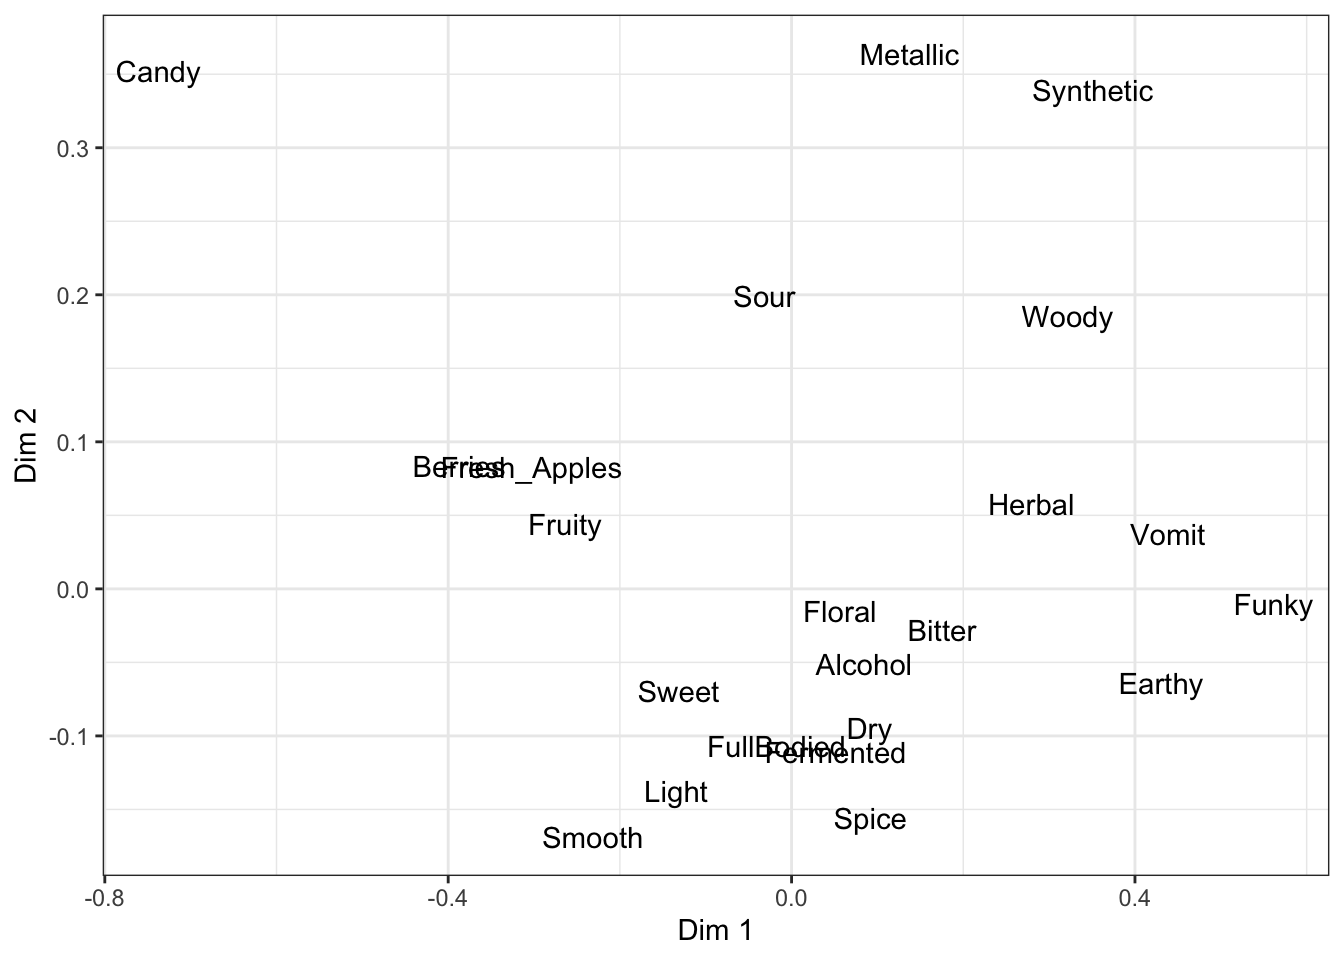
\includegraphics{04-ggplot2-extensions_files/figure-latex/using geom_text with 22 sensory attributes-1} \end{center}

\begin{Shaded}
\begin{Highlighting}[]
\NormalTok{ca\_cider\_termplot }\SpecialCharTok{+}
  \FunctionTok{geom\_label}\NormalTok{()}
\end{Highlighting}
\end{Shaded}

\begin{center}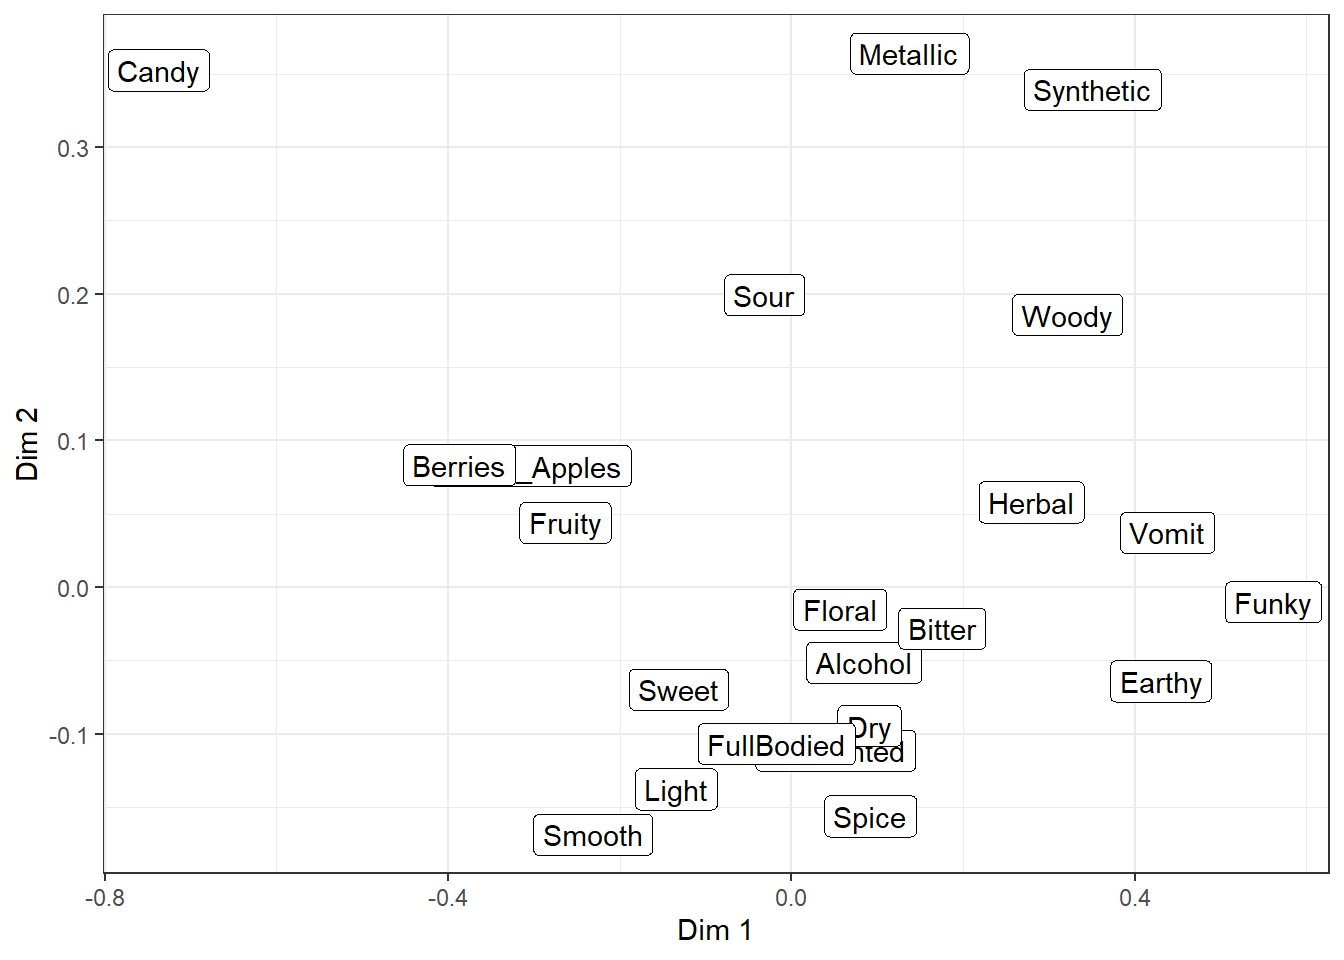
\includegraphics{04-ggplot2-extensions_files/figure-latex/using geom_label with 22 sensory attributes-1} \end{center}

But, as you can see, the text starts to overlap itself quickly even with only a small handful of attributes. The extension I personally use most often, to make crowded plots like this more readable, is the package \texttt{ggrepel}, which adds new \texttt{geom\_text\_repel()} and \texttt{geom\_label\_repel()}.

\begin{Shaded}
\begin{Highlighting}[]
\NormalTok{ca\_cider\_termplot }\SpecialCharTok{+}
\NormalTok{  ggrepel}\SpecialCharTok{::}\FunctionTok{geom\_label\_repel}\NormalTok{()}
\end{Highlighting}
\end{Shaded}

\begin{center}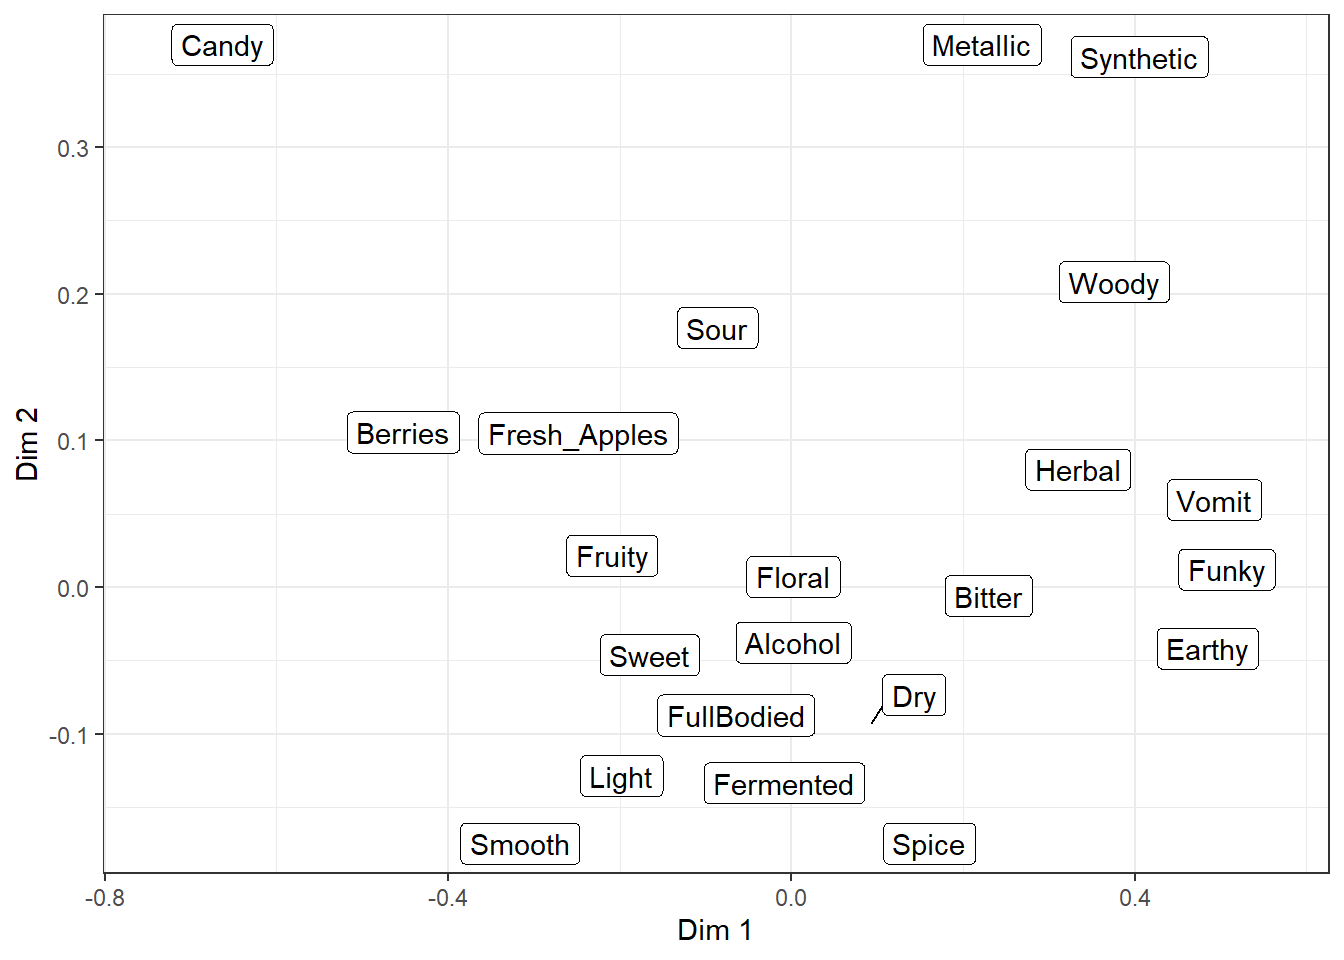
\includegraphics{04-ggplot2-extensions_files/figure-latex/using geom_label_repel with 22 sensory attributes-1} \end{center}

They're almost identical to the normal text and label \texttt{geom\_*()}s, but they use an iterative algorithm to push each piece of text away from the other text and unrelated points or \texttt{geom\_()}s, while being pulled towards the point being labeled. It is \emph{not deterministic}, so it will be slightly different each time you run the code (try it now!) unless you use \texttt{set.seed()} first or set \texttt{seed\ =\ ***} when adding \texttt{geom\_*\_repel()}.

Even with a set seed, changing the plot size or adding \texttt{geom\_*()}s to the plot will also slightly change the locations of the labels, so if you're going to try and find a seed that works well for your data, you should be checking it on your final exported plot at the publication resolution (we'll talk about that next chapter).

\begin{Shaded}
\begin{Highlighting}[]
\NormalTok{ca\_cider\_termplot }\SpecialCharTok{+}
\NormalTok{  ggrepel}\SpecialCharTok{::}\FunctionTok{geom\_label\_repel}\NormalTok{(}\AttributeTok{seed =} \DecValTok{12345}\NormalTok{)}
\end{Highlighting}
\end{Shaded}

\begin{center}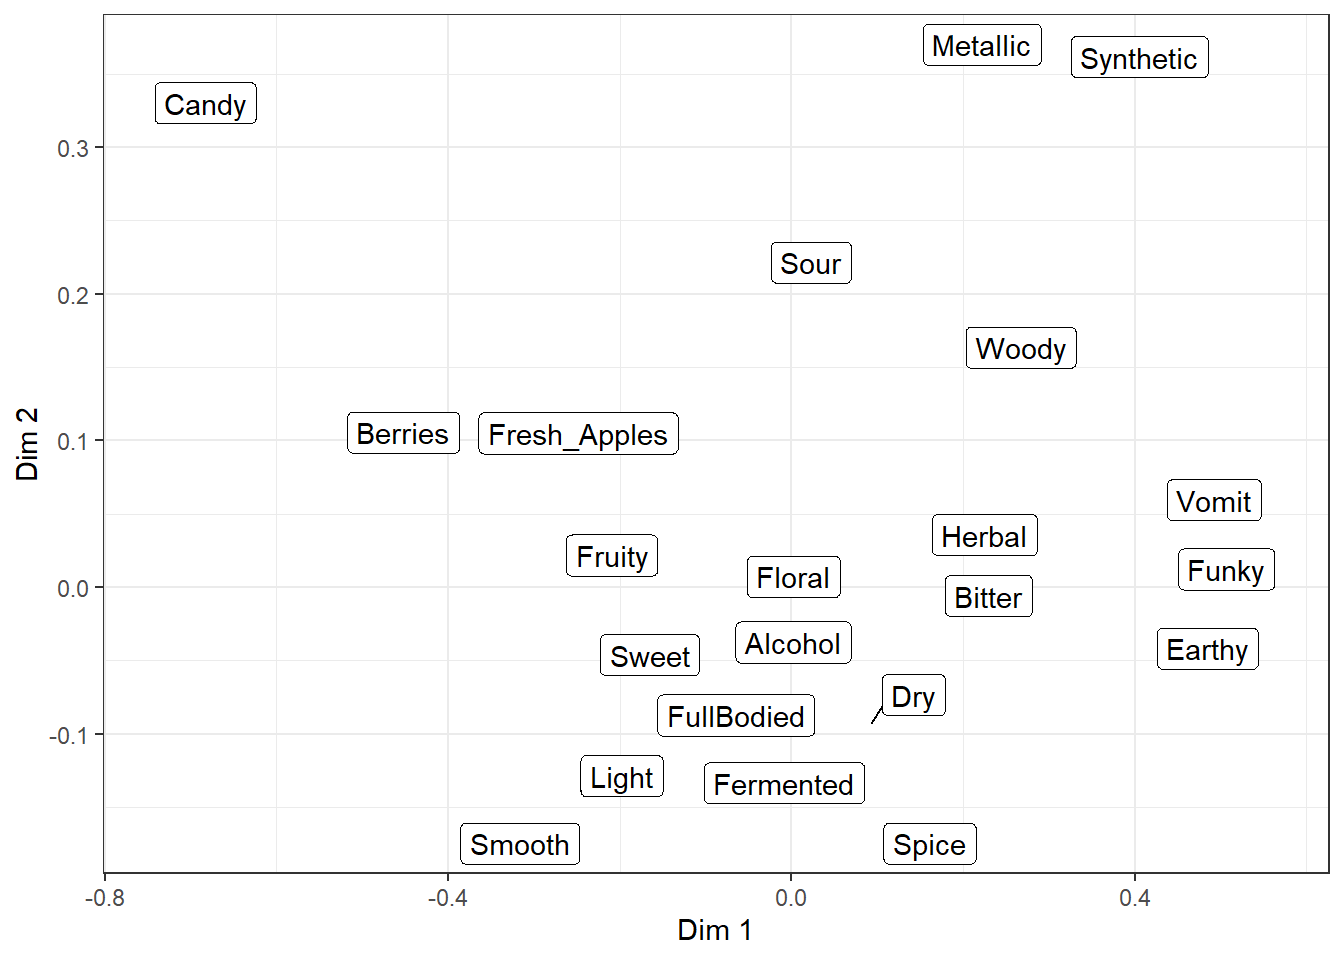
\includegraphics{04-ggplot2-extensions_files/figure-latex/geom_text_repel with a set seed will look the same every time-1} \end{center}

There are many settings you can play with to adjust these forces, how far a label has to move for a line to show up, whether any labels are left off in dense areas, and how long it tries to find a solution. And, randomly, the ability to give each letter-shape a border in a different color, which seems to be totally undocumented in the help files. It can be useful if there are other, multi-colored \texttt{geom\_*()}s in the background.

\begin{Shaded}
\begin{Highlighting}[]
\NormalTok{raw\_cider\_data }\SpecialCharTok{\%\textgreater{}\%}
  \FunctionTok{mutate}\NormalTok{(}\AttributeTok{Product =} \FunctionTok{str\_c}\NormalTok{(Sample\_Name, Temperature, }\AttributeTok{sep =} \StringTok{" "}\NormalTok{)) }\SpecialCharTok{\%\textgreater{}\%}
  \FunctionTok{group\_by}\NormalTok{(Product) }\SpecialCharTok{\%\textgreater{}\%}
  \FunctionTok{summarize}\NormalTok{(}\AttributeTok{Liking =} \FunctionTok{mean}\NormalTok{(Liking)) }\SpecialCharTok{\%\textgreater{}\%}
  \FunctionTok{left\_join}\NormalTok{(ca\_cider}\SpecialCharTok{$}\NormalTok{row}\SpecialCharTok{$}\NormalTok{coord }\SpecialCharTok{\%\textgreater{}\%}
              \FunctionTok{as\_tibble}\NormalTok{(}\AttributeTok{rownames =} \StringTok{"Product"}\NormalTok{)) }\SpecialCharTok{\%\textgreater{}\%}
  \FunctionTok{rename\_with}\NormalTok{(}\SpecialCharTok{\textasciitilde{}} \FunctionTok{str\_replace\_all}\NormalTok{(.x, }\StringTok{" "}\NormalTok{, }\StringTok{"."}\NormalTok{)) }\OtherTok{{-}\textgreater{}}\NormalTok{ ca\_cider\_productcoord}

\CommentTok{\#This is NOT a statistically sound preference model, this is just for demonstration}
\NormalTok{ca\_cider\_prefmod }\OtherTok{\textless{}{-}} \FunctionTok{lm}\NormalTok{(Liking }\SpecialCharTok{\textasciitilde{}}\NormalTok{ Dim}\FloatTok{.1} \SpecialCharTok{*}\NormalTok{ Dim}\FloatTok{.2}\NormalTok{, }\AttributeTok{data =}\NormalTok{ ca\_cider\_productcoord)}
\FunctionTok{expand.grid}\NormalTok{(}\AttributeTok{Dim.1 =} \FunctionTok{seq}\NormalTok{(}\FunctionTok{min}\NormalTok{(ca\_cider}\SpecialCharTok{$}\NormalTok{col}\SpecialCharTok{$}\NormalTok{coord[, }\StringTok{"Dim 1"}\NormalTok{]) }\SpecialCharTok{{-}} \FloatTok{0.1}\NormalTok{,}
                    \FunctionTok{max}\NormalTok{(ca\_cider}\SpecialCharTok{$}\NormalTok{col}\SpecialCharTok{$}\NormalTok{coord[, }\StringTok{"Dim 1"}\NormalTok{]) }\SpecialCharTok{+} \FloatTok{0.1}\NormalTok{,}
                    \AttributeTok{by =} \FloatTok{0.01}\NormalTok{),}
            \AttributeTok{Dim.2 =} \FunctionTok{seq}\NormalTok{(}\FunctionTok{min}\NormalTok{(ca\_cider}\SpecialCharTok{$}\NormalTok{col}\SpecialCharTok{$}\NormalTok{coord[, }\StringTok{"Dim 2"}\NormalTok{]) }\SpecialCharTok{{-}} \FloatTok{0.1}\NormalTok{,}
                    \FunctionTok{max}\NormalTok{(ca\_cider}\SpecialCharTok{$}\NormalTok{col}\SpecialCharTok{$}\NormalTok{coord[, }\StringTok{"Dim 2"}\NormalTok{]) }\SpecialCharTok{+} \FloatTok{0.1}\NormalTok{,}
                    \AttributeTok{by =} \FloatTok{0.01}\NormalTok{)) }\SpecialCharTok{\%\textgreater{}\%}
  \FunctionTok{mutate}\NormalTok{(., }\AttributeTok{Liking =} \FunctionTok{predict}\NormalTok{(ca\_cider\_prefmod, }\AttributeTok{newdata =}\NormalTok{ .)) }\OtherTok{{-}\textgreater{}}\NormalTok{ ca\_cider\_prefinterp}

\NormalTok{ca\_cider\_termplot }\SpecialCharTok{+}
  \FunctionTok{geom\_contour\_filled}\NormalTok{(}\FunctionTok{aes}\NormalTok{(}\AttributeTok{x =}\NormalTok{ Dim}\FloatTok{.1}\NormalTok{, }\AttributeTok{y =}\NormalTok{ Dim}\FloatTok{.2}\NormalTok{, }\AttributeTok{z =}\NormalTok{ Liking, }\AttributeTok{fill =} \FunctionTok{after\_stat}\NormalTok{(level)),}
                  \AttributeTok{inherit.aes =} \ConstantTok{FALSE}\NormalTok{,}
                  \AttributeTok{data =}\NormalTok{ ca\_cider\_prefinterp) }\SpecialCharTok{+} 
  \FunctionTok{scale\_x\_continuous}\NormalTok{(}\AttributeTok{expand =} \FunctionTok{c}\NormalTok{(}\DecValTok{0}\NormalTok{, }\DecValTok{0}\NormalTok{)) }\SpecialCharTok{+}
  \FunctionTok{scale\_y\_continuous}\NormalTok{(}\AttributeTok{expand =} \FunctionTok{c}\NormalTok{(}\DecValTok{0}\NormalTok{, }\DecValTok{0}\NormalTok{)) }\SpecialCharTok{+}
\NormalTok{  ggrepel}\SpecialCharTok{::}\FunctionTok{geom\_text\_repel}\NormalTok{(}\AttributeTok{size =} \DecValTok{6}\NormalTok{, }\AttributeTok{color =} \StringTok{"white"}\NormalTok{, }\AttributeTok{bg.color =} \StringTok{"grey7"}\NormalTok{)}
\end{Highlighting}
\end{Shaded}

\begin{center}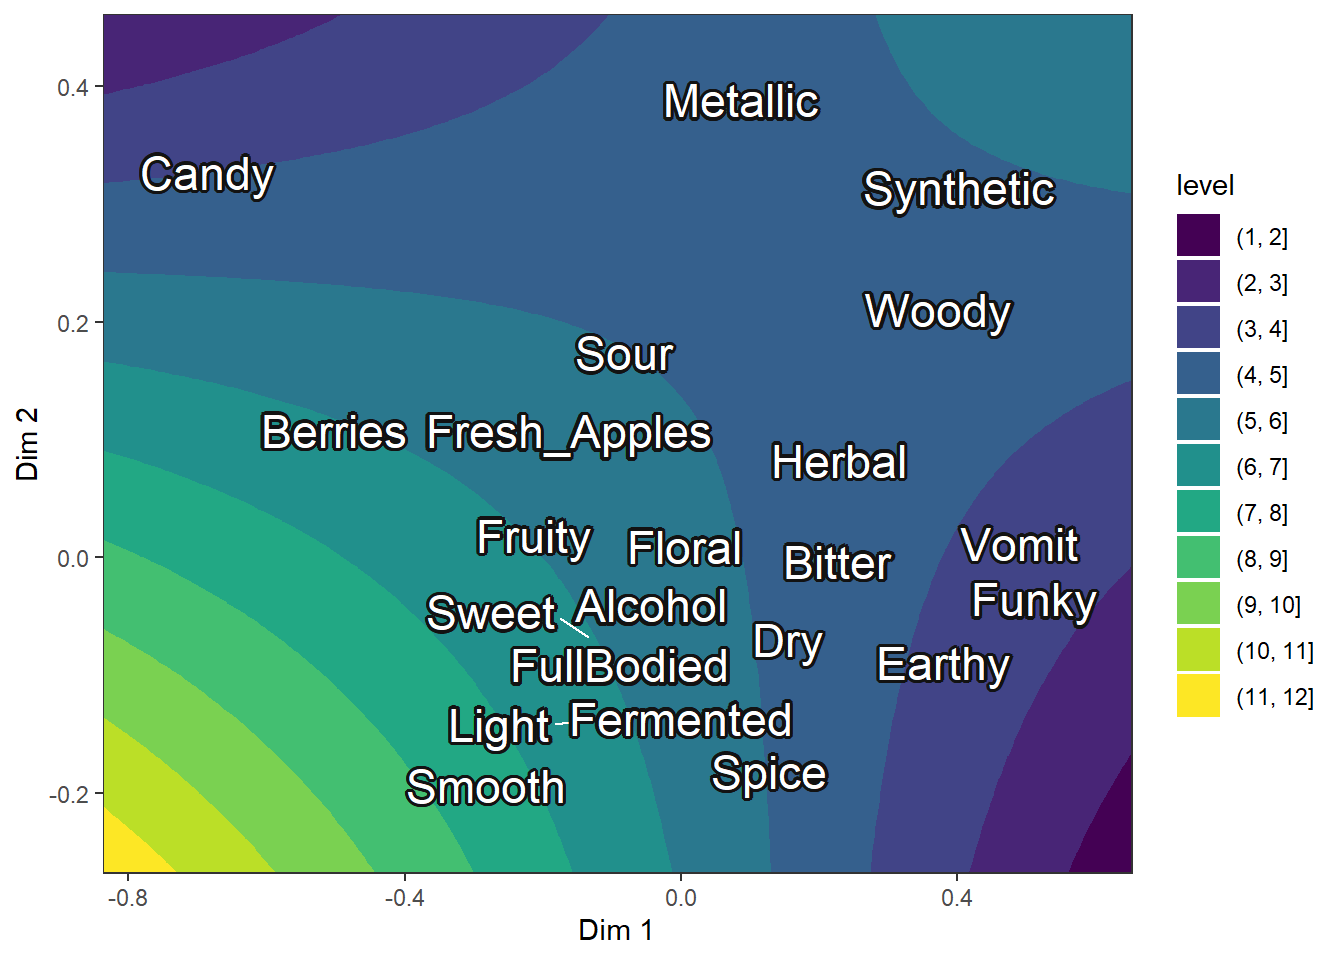
\includegraphics{04-ggplot2-extensions_files/figure-latex/geom_text_repel text borders-1} \end{center}

Another useful tool for visualizing any ordinal/binned data (e.g., the 9-point hedonic scale) at scale is the \texttt{geom\_beeswarm()} and \texttt{geom\_quasirandom()} from the \texttt{ggbeeswarm} package, which are similar to \texttt{geom\_jitter()} but intended for looking at a single numeric variable at a time, possibly across multiple categories.

They limit the jitter to a single direction and ensure that no points are overlapping (or, in the case of \texttt{geom\_quasirandom()}, that there's a uniform amount of overlap) so you can get a more accurate picture of the density, but take up less space than many faceted \texttt{geom\_histogram()}s (at least for the same amount of fine-tuning).

\begin{Shaded}
\begin{Highlighting}[]
\CommentTok{\#The jitter plot is actually not very helpful with this many points}
\NormalTok{berry\_long\_liking }\SpecialCharTok{\%\textgreater{}\%}
  \FunctionTok{ggplot}\NormalTok{(}\FunctionTok{aes}\NormalTok{(}\AttributeTok{x =}\NormalTok{ Scale, }\AttributeTok{y =}\NormalTok{ Liking, }\AttributeTok{color =}\NormalTok{ Scale)) }\SpecialCharTok{+}
  \FunctionTok{geom\_jitter}\NormalTok{() }\SpecialCharTok{+}
  \FunctionTok{facet\_wrap}\NormalTok{(}\SpecialCharTok{\textasciitilde{}}\NormalTok{ Attribute) }\SpecialCharTok{+}
  \FunctionTok{theme\_bw}\NormalTok{()}
\end{Highlighting}
\end{Shaded}

\begin{center}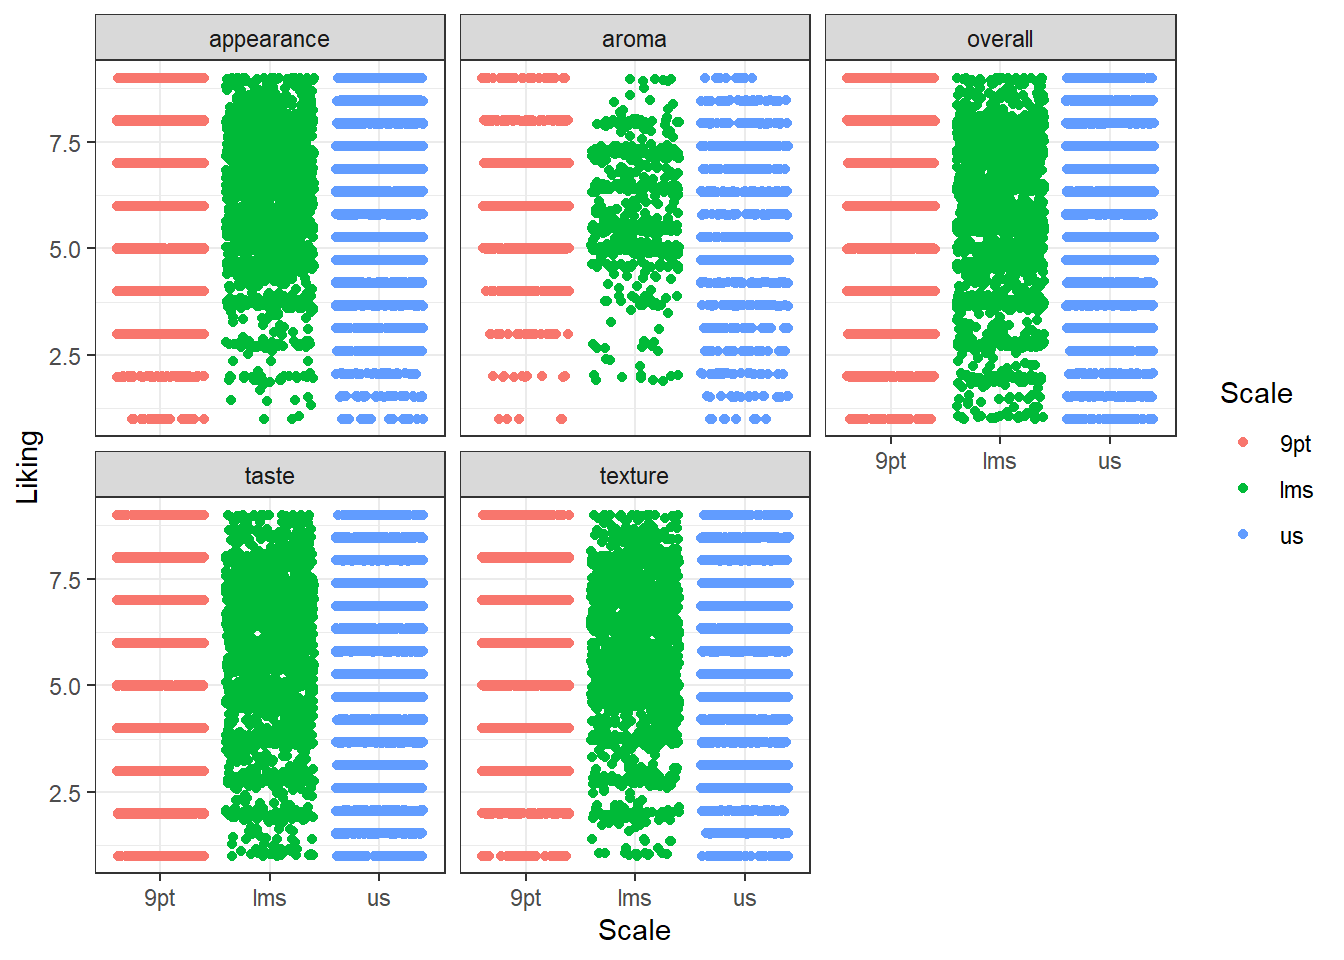
\includegraphics{04-ggplot2-extensions_files/figure-latex/using ggbeeswarm to compare ordinal distributions-1} \end{center}

\begin{Shaded}
\begin{Highlighting}[]
\CommentTok{\#geom\_beeswarm() will also have the same problem, but geom\_quasirandom()}
\CommentTok{\#visualizes the density at each "bin" without us having to specify bins.}
\CommentTok{\#So these are easy to compare}
\NormalTok{berry\_long\_liking }\SpecialCharTok{\%\textgreater{}\%}
  \FunctionTok{ggplot}\NormalTok{(}\FunctionTok{aes}\NormalTok{(}\AttributeTok{x =}\NormalTok{ Scale, }\AttributeTok{y =}\NormalTok{ Liking, }\AttributeTok{color =}\NormalTok{ Scale)) }\SpecialCharTok{+}
\NormalTok{  ggbeeswarm}\SpecialCharTok{::}\FunctionTok{geom\_quasirandom}\NormalTok{() }\SpecialCharTok{+}
  \FunctionTok{facet\_wrap}\NormalTok{(}\SpecialCharTok{\textasciitilde{}}\NormalTok{ Attribute) }\SpecialCharTok{+}
  \FunctionTok{theme\_bw}\NormalTok{()}
\end{Highlighting}
\end{Shaded}

\begin{center}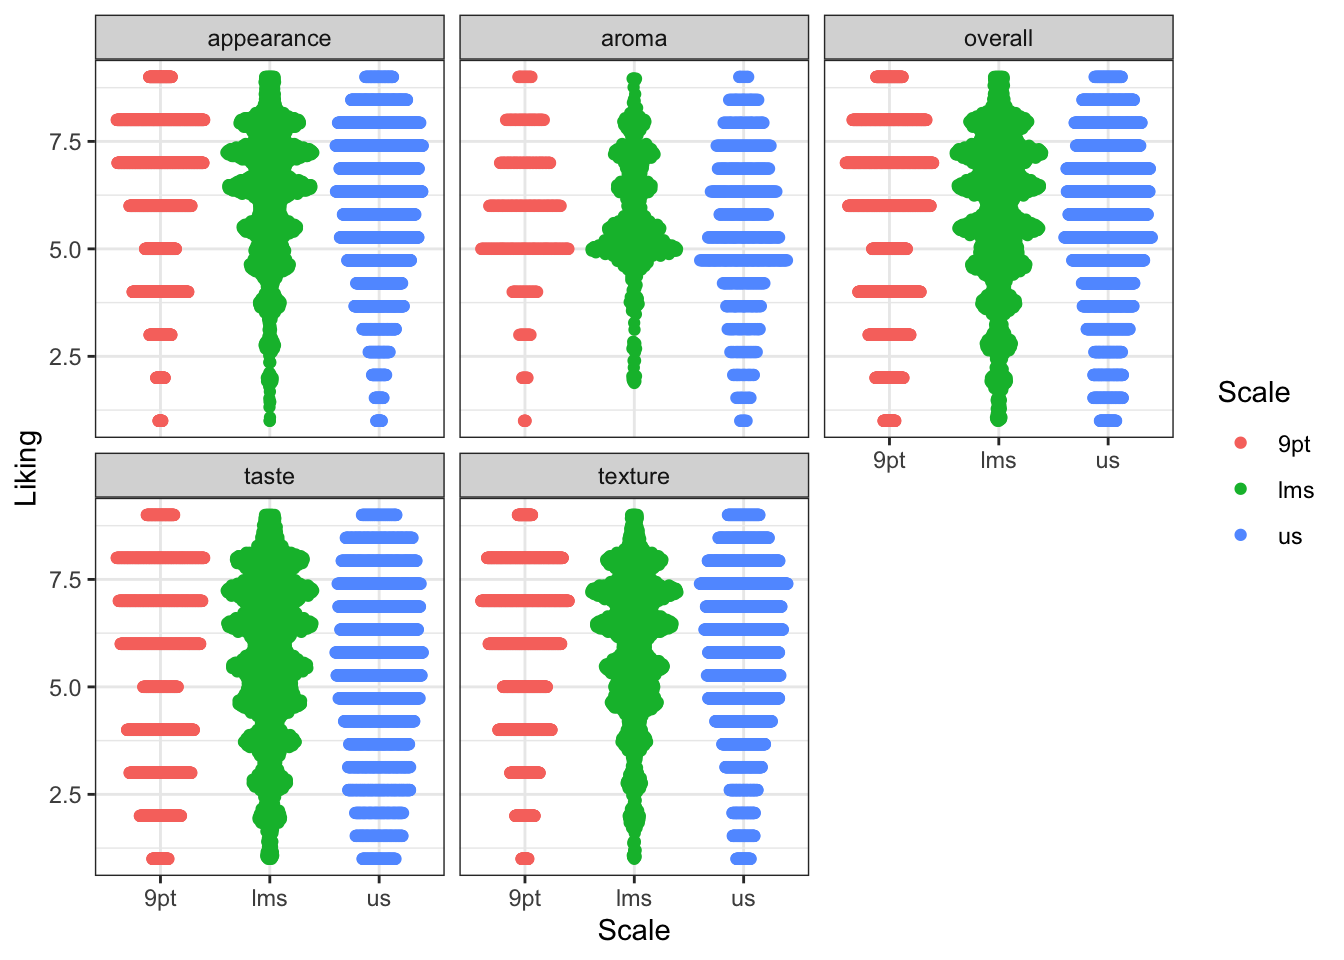
\includegraphics{04-ggplot2-extensions_files/figure-latex/using ggbeeswarm to compare ordinal distributions-2} \end{center}

If you want to easily add circles and ellipses to a plot (say, the unit circle or a confidence ellipse), you'll probably want to install the \texttt{ggforce} package and use \texttt{geom\_circle()} or \texttt{geom\_ellipse()}, respectively.

\begin{Shaded}
\begin{Highlighting}[]
\NormalTok{berry\_mfa\_res}\SpecialCharTok{$}\NormalTok{quanti.var}\SpecialCharTok{$}\NormalTok{coord }\SpecialCharTok{\%\textgreater{}\%}
  \FunctionTok{as\_tibble}\NormalTok{(}\AttributeTok{rownames =} \StringTok{"Modality"}\NormalTok{) }\SpecialCharTok{\%\textgreater{}\%}
  \FunctionTok{ggplot}\NormalTok{() }\SpecialCharTok{+}
  \FunctionTok{geom\_segment}\NormalTok{(}\FunctionTok{aes}\NormalTok{(}\AttributeTok{x =} \DecValTok{0}\NormalTok{, }\AttributeTok{y =} \DecValTok{0}\NormalTok{, }\AttributeTok{xend =}\NormalTok{ Dim}\FloatTok{.1}\NormalTok{, }\AttributeTok{yend =}\NormalTok{ Dim}\FloatTok{.2}\NormalTok{), }\AttributeTok{arrow =} \FunctionTok{arrow}\NormalTok{()) }\SpecialCharTok{+}
\NormalTok{  ggforce}\SpecialCharTok{::}\FunctionTok{geom\_circle}\NormalTok{(}\FunctionTok{aes}\NormalTok{(}\AttributeTok{x0 =} \DecValTok{0}\NormalTok{, }\AttributeTok{y0 =} \DecValTok{0}\NormalTok{, }\AttributeTok{r =} \DecValTok{1}\NormalTok{), }\AttributeTok{color =} \StringTok{"blue"}\NormalTok{) }\SpecialCharTok{+}
\NormalTok{  ggrepel}\SpecialCharTok{::}\FunctionTok{geom\_text\_repel}\NormalTok{(}\FunctionTok{aes}\NormalTok{(}\AttributeTok{x =}\NormalTok{ Dim}\FloatTok{.1}\NormalTok{, }\AttributeTok{y =}\NormalTok{ Dim}\FloatTok{.2}\NormalTok{, }\AttributeTok{label =}\NormalTok{ Modality)) }\SpecialCharTok{+}
  \FunctionTok{theme\_bw}\NormalTok{() }\SpecialCharTok{+}
  \FunctionTok{theme}\NormalTok{(}\AttributeTok{aspect.ratio =} \DecValTok{1}\NormalTok{)}
\end{Highlighting}
\end{Shaded}

\begin{center}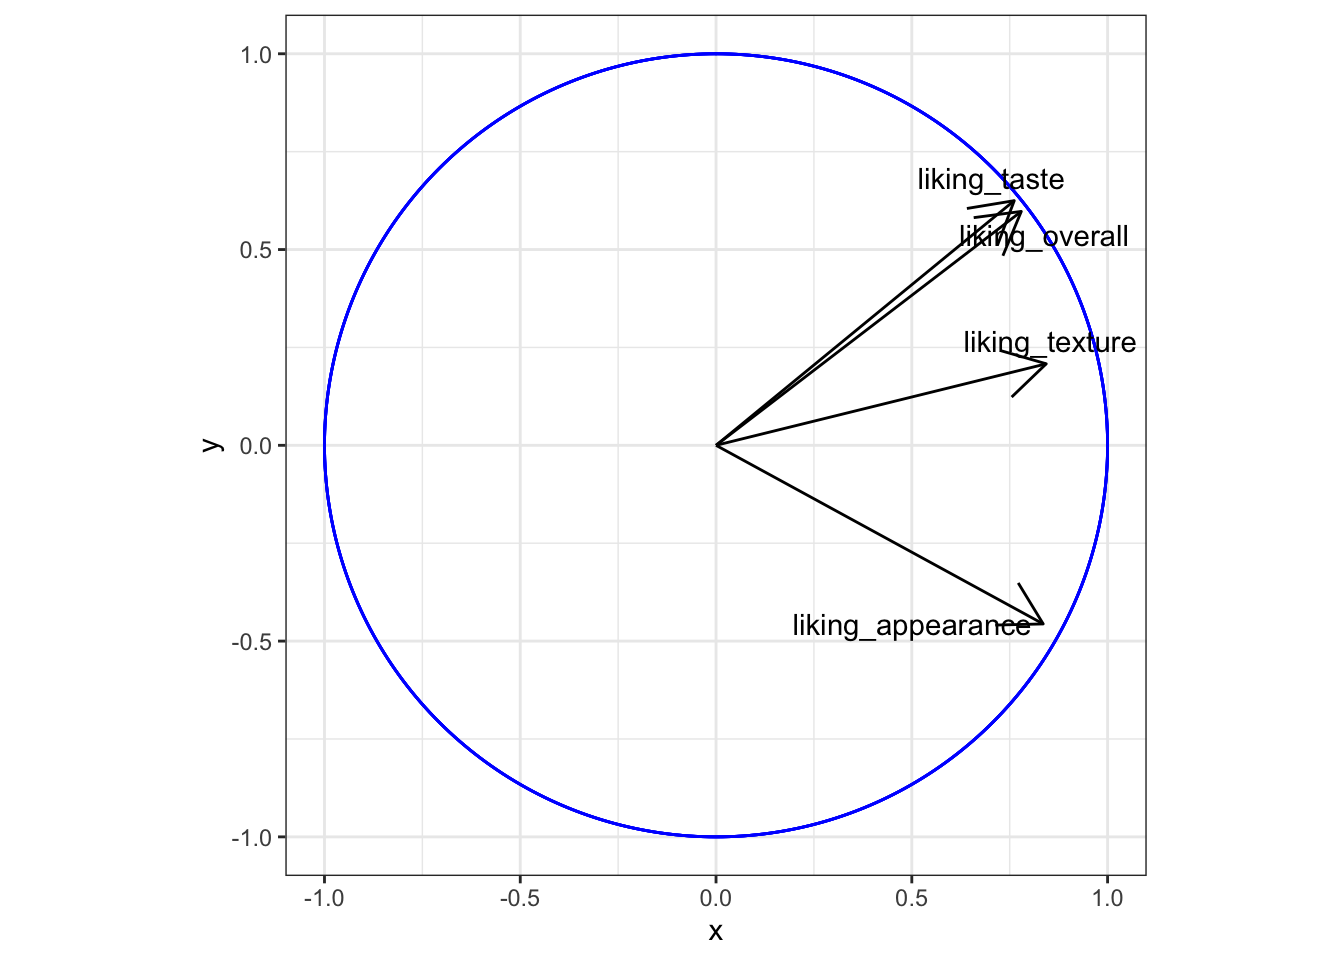
\includegraphics{04-ggplot2-extensions_files/figure-latex/adding a unit circle with ggforce-1} \end{center}

\hypertarget{new-theme_s-and-scale_s}{%
\section{\texorpdfstring{New \texttt{theme\_*()}s and \texttt{scale\_*()}s}{New theme\_*()s and scale\_*()s}}\label{new-theme_s-and-scale_s}}

Most of the additional \texttt{geom\_*()}s in \texttt{ggplot2} extensions involve some sort of calculation, so the confidence that you're using someone else's algorithm that's (hopefully!) been double-checked is a real benefit. You've already seen how to change the way your plots look with \texttt{theme()} one argument at a time, and how to set \texttt{scale\_*\_manual()} if you have the exact colors or color range that you want.

So there's nothing these prettying-up packages will do that you can't do yourself, but there are a huge number of \texttt{ggplot2} extensions that include some version of a no-gridline minimal theme for convenience. Such as:

\begin{Shaded}
\begin{Highlighting}[]
\NormalTok{berry\_long\_liking }\SpecialCharTok{\%\textgreater{}\%}
  \FunctionTok{ggplot}\NormalTok{(}\FunctionTok{aes}\NormalTok{(}\AttributeTok{x =}\NormalTok{ Scale, }\AttributeTok{y =}\NormalTok{ Liking, }\AttributeTok{color =}\NormalTok{ Scale)) }\SpecialCharTok{+}
\NormalTok{  ggbeeswarm}\SpecialCharTok{::}\FunctionTok{geom\_quasirandom}\NormalTok{() }\SpecialCharTok{+}
  \FunctionTok{facet\_wrap}\NormalTok{(}\SpecialCharTok{\textasciitilde{}}\NormalTok{ Attribute) }\SpecialCharTok{+}
\NormalTok{  cowplot}\SpecialCharTok{::}\FunctionTok{theme\_minimal\_hgrid}\NormalTok{()}
\end{Highlighting}
\end{Shaded}

\begin{center}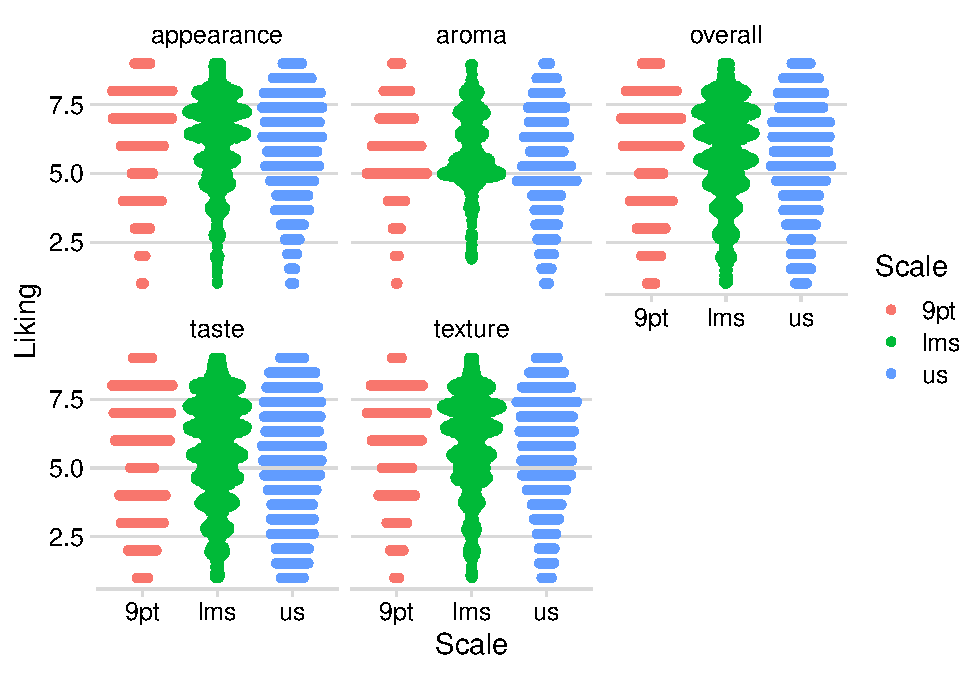
\includegraphics{04-ggplot2-extensions_files/figure-latex/the minimal themes in cowplot-1} \end{center}

Packages that added \texttt{scale\_*()}s used to be one of the most common kinds of ggplot extensions (because, as you'll notice, the above figure with the default color scale is not red-green colorblind friendly), but the most popular scales now come with \texttt{ggplot2} itself.

\texttt{RColorBrewer}'s colorblind- and printer-friendly palettes for categorical data are now available in \texttt{ggplot2::scale\_*\_brewer\_*()}, and you've already seen us use the \texttt{viridis} color palettes in \texttt{ggplot2::scale\_*\_viridis\_*()}. The \texttt{viridis} color scales \emph{can} be used for categorical data, if you use the \texttt{\_d()} versions, but they were designed for ordinal and binned data, since some colors will seem more related than others. See \href{https://clauswilke.com/dataviz/color-basics.html}{Chapter 4} and \href{https://clauswilke.com/dataviz/color-pitfalls.html}{Chapter 19} of Claus O. Wilke's book \emph{Fundamentals of Data Visualization}.

\hypertarget{modifying-ggplots-made-by-other-packages}{%
\section{\texorpdfstring{Modifying \texttt{ggplot()}s made by other packages}{Modifying ggplot()s made by other packages}}\label{modifying-ggplots-made-by-other-packages}}

So far in this chapter, we've been making all of the plots with a call to \texttt{ggplot()} and then adding on geoms, themes, labels, scales, and facets with \texttt{+}. But we've also been able to save our plots to variables partway through and then keep adding things to the saved plots. This is an incredibly useful difference from the way plots work in base R.

Some packages utilize \texttt{ggplot2} by making a whole plot for you with their own internal call to \texttt{ggplot()}, which means that you can treat it like any other ggplot for the sake of customizing. Most packages which can save a whole plot to a variable or output several plots in a list use \texttt{ggplot()} to do so.

\begin{Shaded}
\begin{Highlighting}[]
\CommentTok{\#FactoMineR uses ggplot for its internal plotting,}
\CommentTok{\#Which is why we can assign the output to a variable}
\CommentTok{\#and not see the plot right away}
\CommentTok{\#(although the CA() function will also display several plots by default)}
\NormalTok{cider\_contingency }\SpecialCharTok{\%\textgreater{}\%}
\NormalTok{  FactoMineR}\SpecialCharTok{::}\FunctionTok{CA}\NormalTok{(}\AttributeTok{graph =} \ConstantTok{FALSE}\NormalTok{) }\SpecialCharTok{\%\textgreater{}\%}
\NormalTok{  FactoMineR}\SpecialCharTok{::}\FunctionTok{plot.CA}\NormalTok{() }\OtherTok{{-}\textgreater{}}\NormalTok{ ca\_cider\_biplot\_facto}

\CommentTok{\#The ca package, meanwhile, uses base plotting.}
\CommentTok{\#You can tell because it prints this plot immediately.}
\NormalTok{cider\_contingency }\SpecialCharTok{\%\textgreater{}\%}
\NormalTok{  ca}\SpecialCharTok{::}\FunctionTok{ca}\NormalTok{() }\SpecialCharTok{\%\textgreater{}\%}
\NormalTok{  ca}\SpecialCharTok{::}\FunctionTok{plot.ca}\NormalTok{() }\OtherTok{{-}\textgreater{}}\NormalTok{ ca\_cider\_biplot\_green}
\end{Highlighting}
\end{Shaded}

\begin{center}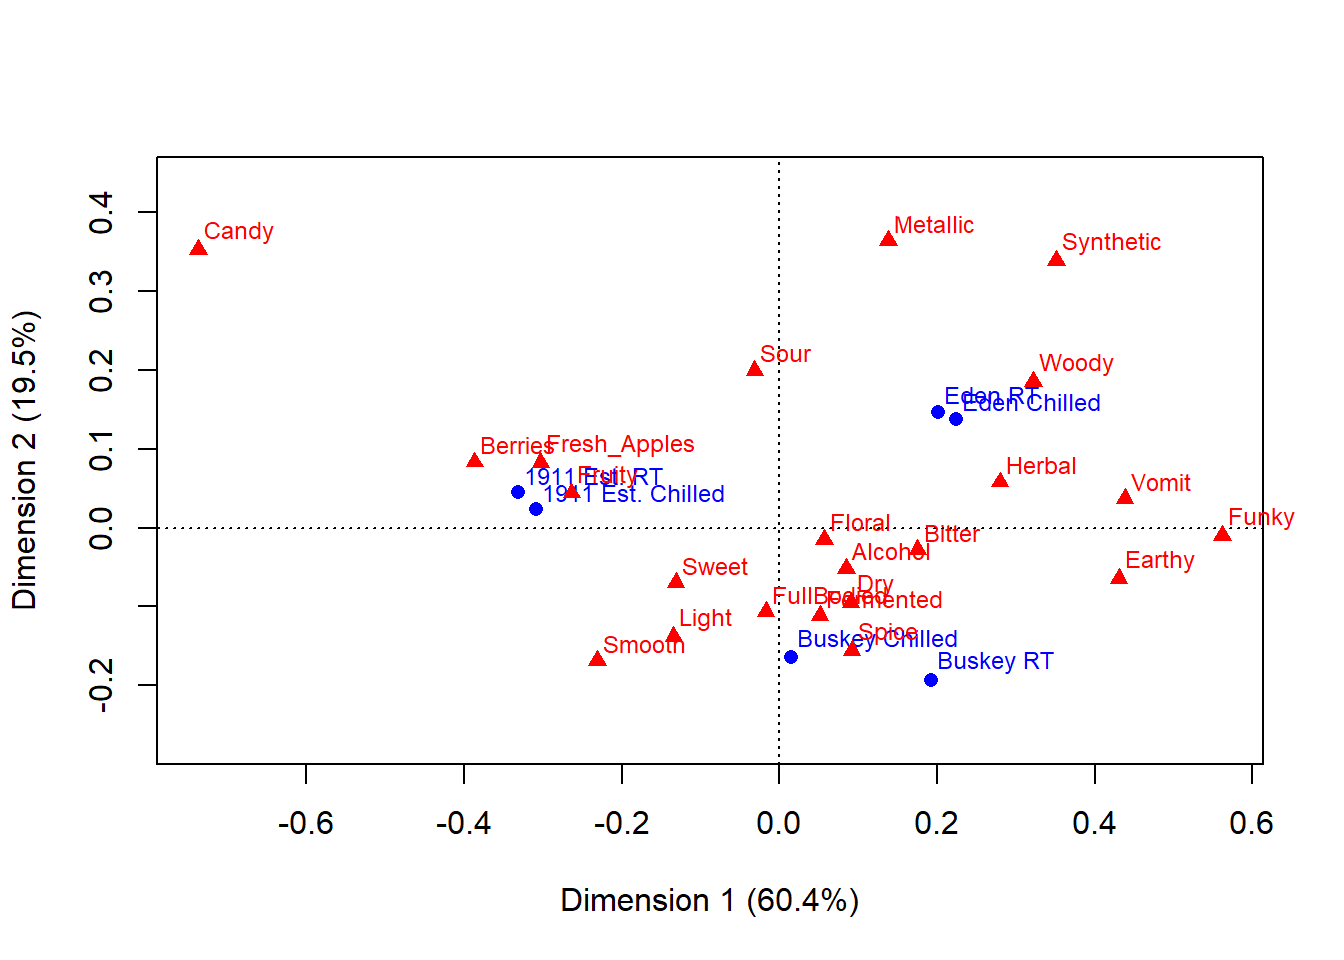
\includegraphics{04-ggplot2-extensions_files/figure-latex/FactoMineR makes ggplots-1} \end{center}

You can see that the last code chunk only output one plot right away, but we can confirm our suspicions with the base \texttt{R} \texttt{class()} function.

\begin{Shaded}
\begin{Highlighting}[]
\FunctionTok{class}\NormalTok{(ca\_cider\_termplot) }\CommentTok{\# Made with ggplot() ourselves}
\end{Highlighting}
\end{Shaded}

\begin{verbatim}
## [1] "gg"     "ggplot"
\end{verbatim}

\begin{Shaded}
\begin{Highlighting}[]
\FunctionTok{class}\NormalTok{(ca\_cider\_biplot\_facto) }\CommentTok{\# Made with ggplot{-}based FactoMineR}
\end{Highlighting}
\end{Shaded}

\begin{verbatim}
## [1] "gg"     "ggplot"
\end{verbatim}

\begin{Shaded}
\begin{Highlighting}[]
\FunctionTok{class}\NormalTok{(ca\_cider\_biplot\_green) }\CommentTok{\# Made with ca::ca(), not a plot at all}
\end{Highlighting}
\end{Shaded}

\begin{verbatim}
## [1] "list"
\end{verbatim}

\begin{Shaded}
\begin{Highlighting}[]
\NormalTok{ca\_cider\_biplot\_green }\CommentTok{\# It\textquotesingle{}s two tables of coordinates!}
\end{Highlighting}
\end{Shaded}

\begin{verbatim}
## $rows
##                          Dim1        Dim2
## 1911 Est. Chilled -0.30922746  0.02323046
## 1911 Est. RT      -0.33096663  0.04492088
## Buskey Chilled     0.01508206 -0.16463573
## Buskey RT          0.19222871 -0.19341072
## Eden Chilled       0.22460300  0.13702229
## Eden RT            0.20122093  0.14661009
## 
## $cols
##                     Dim1        Dim2
## Fresh_Apples -0.30305451  0.08260444
## Fermented     0.05136995 -0.11123214
## Herbal        0.27953814  0.05798442
## Dry           0.09068713 -0.09458987
## Spice         0.09194648 -0.15607561
## Fruity       -0.26360780  0.04401256
## Smooth       -0.23141023 -0.16865980
## Alcohol       0.08456228 -0.05135981
## Light        -0.13444990 -0.13768159
## Sweet        -0.13152453 -0.06963735
## Woody         0.32164765  0.18574435
## Berries      -0.38694032  0.08324652
## Sour         -0.03153644  0.19917586
## Funky         0.56153039 -0.01014260
## FullBodied   -0.01727177 -0.10673686
## Metallic      0.13770506  0.36391448
## Floral        0.05665116 -0.01517803
## Candy        -0.73752932  0.35245085
## Bitter        0.17535866 -0.02812715
## Vomit         0.43823154  0.03719609
## Earthy        0.43043925 -0.06405187
## Synthetic     0.35094003  0.33924051
\end{verbatim}

What this means is that we can look at the \texttt{FactoMineR}-made plot we've saved to \texttt{ca\_cider\_biplot\_facto}:

\begin{Shaded}
\begin{Highlighting}[]
\NormalTok{ca\_cider\_biplot\_facto}
\end{Highlighting}
\end{Shaded}

\begin{center}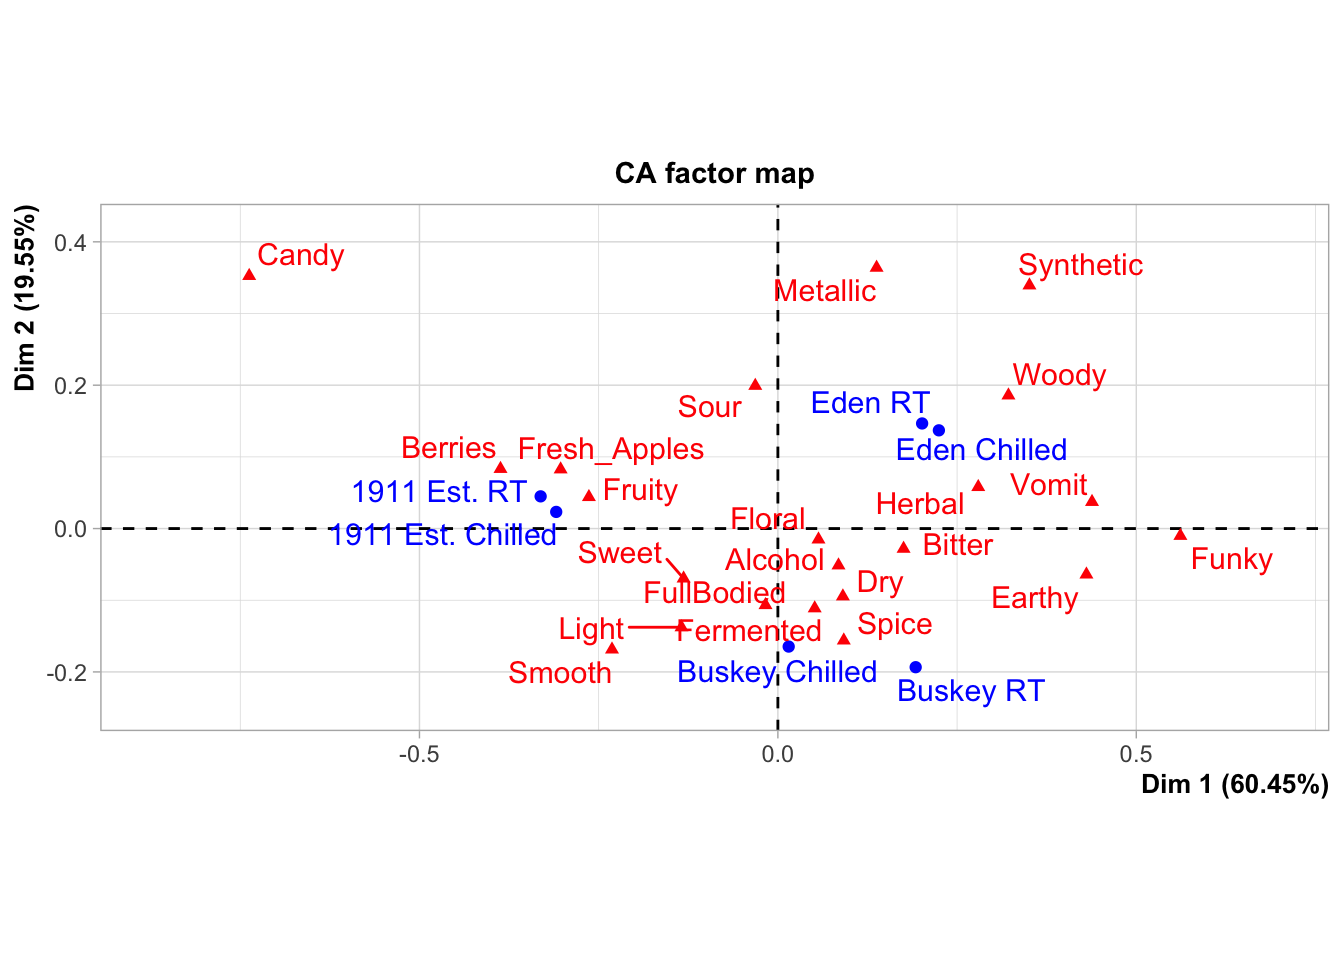
\includegraphics{04-ggplot2-extensions_files/figure-latex/you can see saved ggplots by calling the variable-1} \end{center}

\emph{And} we can still change up many of the elements by adding additional elements, although you're likely to get some weird warning messages \emph{and} some silent errors. (The \texttt{ggrepel} error message is actually just because there are too many \texttt{geom\_text\_repel()} labels close-together in a small plots, because expanding \texttt{xlim()} crowds everything in the center of the plot.)

\begin{Shaded}
\begin{Highlighting}[]
\NormalTok{ca\_cider\_biplot\_facto }\SpecialCharTok{+}
  \FunctionTok{theme}\NormalTok{(}\AttributeTok{panel.grid =} \FunctionTok{element\_blank}\NormalTok{(), }\CommentTok{\# Removes the axis lines}
        \AttributeTok{plot.title =} \FunctionTok{element\_blank}\NormalTok{()) }\SpecialCharTok{+} \CommentTok{\# Removes the title}
  \FunctionTok{xlim}\NormalTok{(}\SpecialCharTok{{-}}\DecValTok{1}\NormalTok{,}\DecValTok{1}\NormalTok{) }\SpecialCharTok{+} \CommentTok{\# Extends the x limits, with a warning}
  \FunctionTok{scale\_color\_brewer}\NormalTok{(}\AttributeTok{type =} \StringTok{"qual"}\NormalTok{, }\AttributeTok{palette =} \StringTok{"Dark2"}\NormalTok{)}
\end{Highlighting}
\end{Shaded}

\begin{verbatim}
## Scale for x is already present.
## Adding another scale for x, which will replace the existing scale.
\end{verbatim}

\begin{center}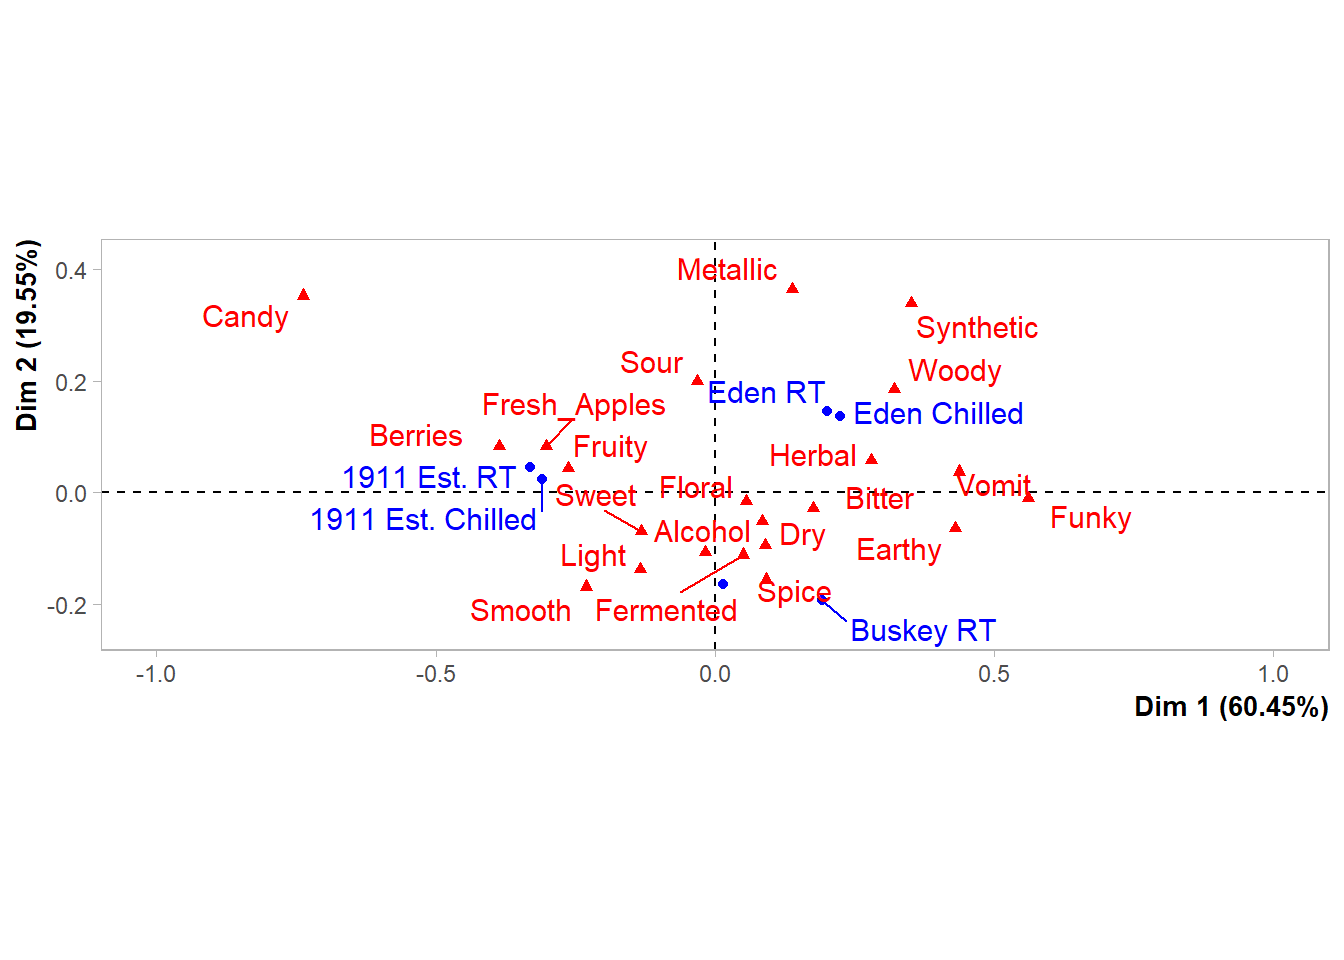
\includegraphics{04-ggplot2-extensions_files/figure-latex/you can change many things about FactoMineR plots with ggplot semantics-1} \end{center}

\begin{Shaded}
\begin{Highlighting}[]
  \CommentTok{\# Silently fails to change the color scale}
\end{Highlighting}
\end{Shaded}

You can't just \texttt{+\ scale\_color\_*()} to a \texttt{FactoMineR} plot, because the \texttt{ggplot} already has a non-default color scheme and adding a second color scale does nothing. If you look at the help file for \texttt{?FactoMineR::plot.CA}, you can set several styling parameters when you're making the plot, and you can remake it as many times as you need, but doing so does have significantly less flexibility than the approach to plotting we've outlined in this workshop.

We also can't go back and adjust the parameters passed to \texttt{geom\_text\_repel()} after the fact, even though we can tell from the warning messages that that's the package being used to put the attribute and product names onto the biplot.

It will almost always be possible to add more \texttt{geom\_*()}s to plots made by other packages, as long as you don't mind them being added \emph{on top of} any existing elements in the plot.

\begin{Shaded}
\begin{Highlighting}[]
\NormalTok{liking\_arrow }\OtherTok{\textless{}{-}} \FunctionTok{data.frame}\NormalTok{(}\AttributeTok{x1 =} \DecValTok{0}\NormalTok{, }\AttributeTok{y1 =} \DecValTok{0}\NormalTok{, }\AttributeTok{x2 =} \SpecialCharTok{{-}}\FloatTok{0.4}\NormalTok{, }\AttributeTok{y2 =} \SpecialCharTok{{-}}\FloatTok{0.1}\NormalTok{, }\AttributeTok{text =} \StringTok{"Liking"}\NormalTok{)}

\NormalTok{ca\_cider\_biplot\_facto }\SpecialCharTok{+}
  \FunctionTok{geom\_segment}\NormalTok{(}\FunctionTok{aes}\NormalTok{(}\AttributeTok{x=}\NormalTok{ x1, }\AttributeTok{y =}\NormalTok{ y1, }\AttributeTok{xend =}\NormalTok{ x2, }\AttributeTok{yend =}\NormalTok{ y2), }\AttributeTok{color =} \StringTok{"orange"}\NormalTok{,}
               \AttributeTok{arrow =} \FunctionTok{arrow}\NormalTok{(}\AttributeTok{length =} \FunctionTok{unit}\NormalTok{(}\FloatTok{0.03}\NormalTok{, }\StringTok{"npc"}\NormalTok{)), }\AttributeTok{linewidth =} \DecValTok{1}\NormalTok{,}
               \AttributeTok{data =}\NormalTok{ liking\_arrow) }\SpecialCharTok{+}
  \FunctionTok{geom\_text}\NormalTok{(}\FunctionTok{aes}\NormalTok{(}\AttributeTok{x =}\NormalTok{ x2, }\AttributeTok{y =}\NormalTok{ y2, }\AttributeTok{label =}\NormalTok{ text), }\AttributeTok{color =} \StringTok{"orange"}\NormalTok{,}
            \AttributeTok{hjust =} \StringTok{"outward"}\NormalTok{, }\AttributeTok{vjust =} \StringTok{"outward"}\NormalTok{, }\AttributeTok{fontface =} \StringTok{"italic"}\NormalTok{,}
            \AttributeTok{data =}\NormalTok{ liking\_arrow)}
\end{Highlighting}
\end{Shaded}

\begin{center}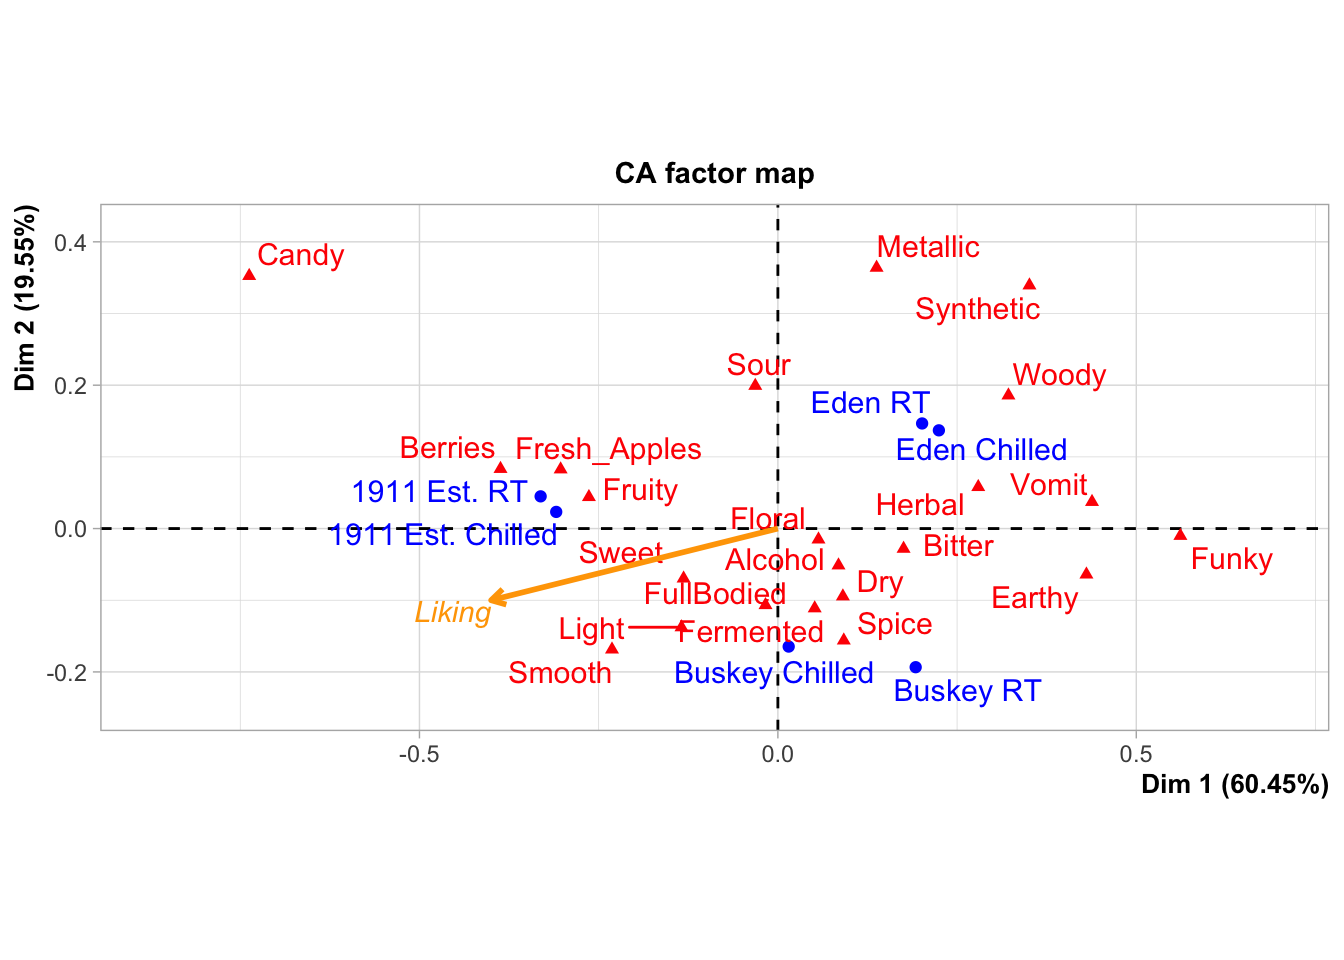
\includegraphics{04-ggplot2-extensions_files/figure-latex/you can easily add new geoms to FactoMineR plots-1} \end{center}

If you desperately need to \href{https://cran.r-project.org/web/packages/gginnards/vignettes/user-guide-2.html\#replacing-scales-coordinates-whole-themes-and-data.}{change a scale or reorder \texttt{geom\_*()}s from an existing \texttt{ggplot}} in a hurry, look into the \texttt{gginnards} package.

\hypertarget{combining-plots}{%
\section{Combining Plots}\label{combining-plots}}

You've already seen how to \texttt{facet\_*()} plots to view ``small multiple'' plots side-by side:

\begin{Shaded}
\begin{Highlighting}[]
\NormalTok{raw\_cider\_data }\SpecialCharTok{\%\textgreater{}\%}
  \FunctionTok{pivot\_longer}\NormalTok{(Fresh\_Apples}\SpecialCharTok{:}\NormalTok{Synthetic) }\SpecialCharTok{\%\textgreater{}\%}
  \FunctionTok{group\_by}\NormalTok{(Sample\_Name, Temperature, name) }\SpecialCharTok{\%\textgreater{}\%}
  \FunctionTok{summarize}\NormalTok{(}\AttributeTok{total =} \FunctionTok{sum}\NormalTok{(value)) }\SpecialCharTok{\%\textgreater{}\%}
  \FunctionTok{ggplot}\NormalTok{(}\FunctionTok{aes}\NormalTok{(}\AttributeTok{x =} \FunctionTok{interaction}\NormalTok{(Sample\_Name, Temperature), }\AttributeTok{y =}\NormalTok{ total)) }\SpecialCharTok{+} 
  \FunctionTok{geom\_col}\NormalTok{(}\FunctionTok{aes}\NormalTok{(}\AttributeTok{fill =}\NormalTok{ Sample\_Name)) }\SpecialCharTok{+}
  \FunctionTok{scale\_fill\_manual}\NormalTok{(}\AttributeTok{values =}\NormalTok{ wesanderson}\SpecialCharTok{::}\NormalTok{wes\_palettes}\SpecialCharTok{$}\NormalTok{FantasticFox1) }\SpecialCharTok{+} 
  \FunctionTok{coord\_flip}\NormalTok{() }\SpecialCharTok{+} 
  \FunctionTok{labs}\NormalTok{(}\AttributeTok{x =} \ConstantTok{NULL}\NormalTok{, }\AttributeTok{y =} \ConstantTok{NULL}\NormalTok{, }\AttributeTok{fill =} \ConstantTok{NULL}\NormalTok{) }\SpecialCharTok{+}
  \FunctionTok{theme\_bw}\NormalTok{() }\SpecialCharTok{+} 
  \FunctionTok{theme}\NormalTok{(}\AttributeTok{legend.position =} \StringTok{"top"}\NormalTok{,}
        \AttributeTok{panel.grid =} \FunctionTok{element\_blank}\NormalTok{()) }\OtherTok{{-}\textgreater{}}\NormalTok{ cider\_count\_plot}

\NormalTok{cider\_count\_plot }\SpecialCharTok{+}
  \FunctionTok{facet\_wrap}\NormalTok{(}\SpecialCharTok{\textasciitilde{}}\NormalTok{name, }\AttributeTok{ncol =} \DecValTok{6}\NormalTok{)}
\end{Highlighting}
\end{Shaded}

\begin{center}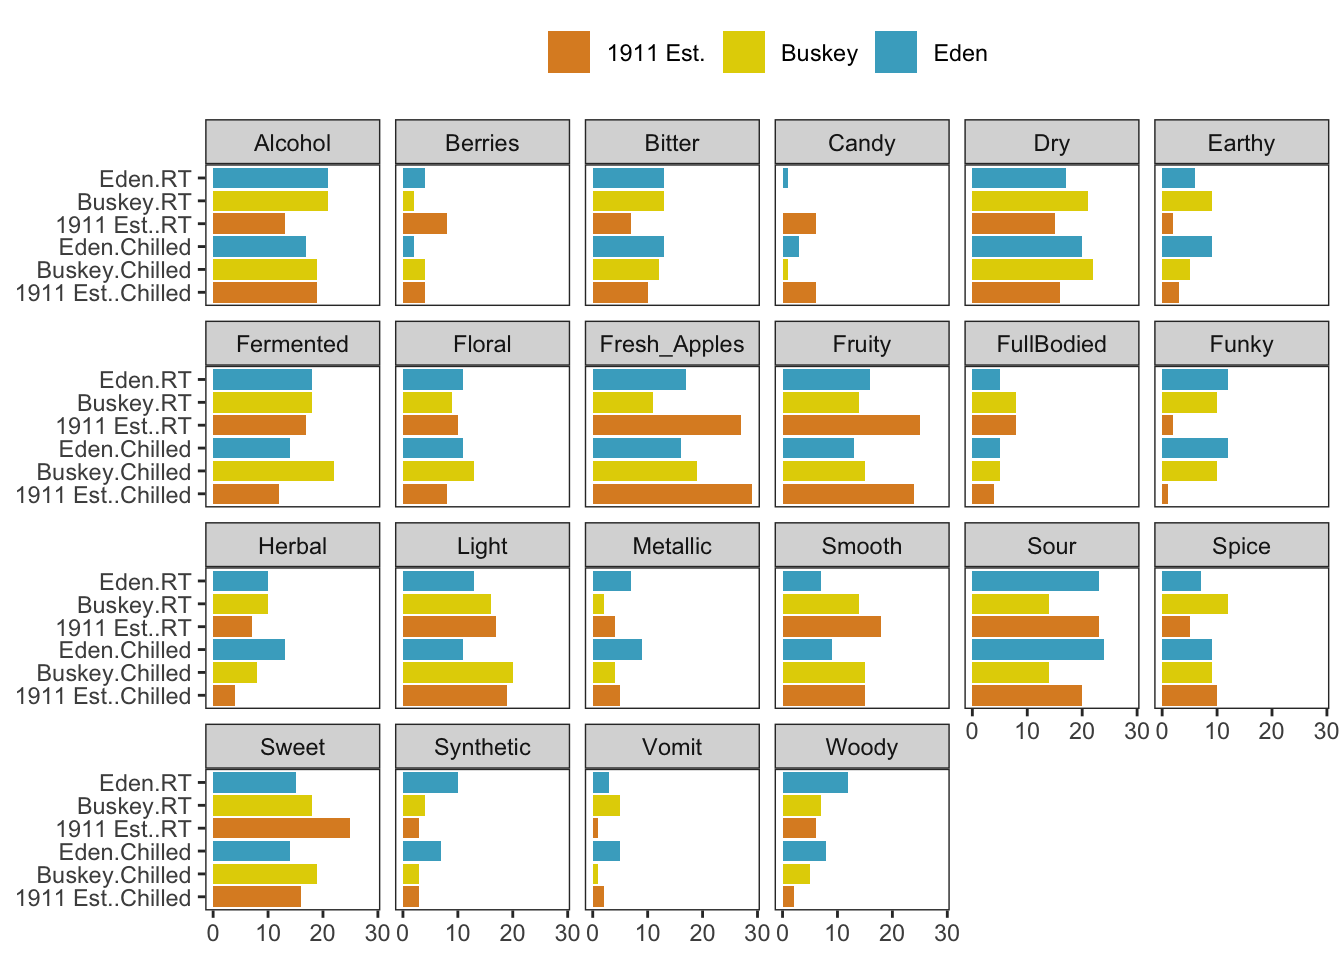
\includegraphics{04-ggplot2-extensions_files/figure-latex/remember faceting-1} \end{center}

This works very well whenever you have multiple plots using the same \texttt{geom\_*()}s that you want to show on the same axes, and you can even adjust the axis limits from facet to facet using \texttt{scales\ =\ "free*"}:

\begin{Shaded}
\begin{Highlighting}[]
\NormalTok{cider\_count\_plot }\SpecialCharTok{+}
  \FunctionTok{facet\_wrap}\NormalTok{(}\SpecialCharTok{\textasciitilde{}}\NormalTok{name, }\AttributeTok{ncol =} \DecValTok{6}\NormalTok{,}
             \AttributeTok{scales =} \StringTok{"free\_x"}\NormalTok{) }\CommentTok{\# Each plot now has a different x{-}axis}
\end{Highlighting}
\end{Shaded}

\begin{center}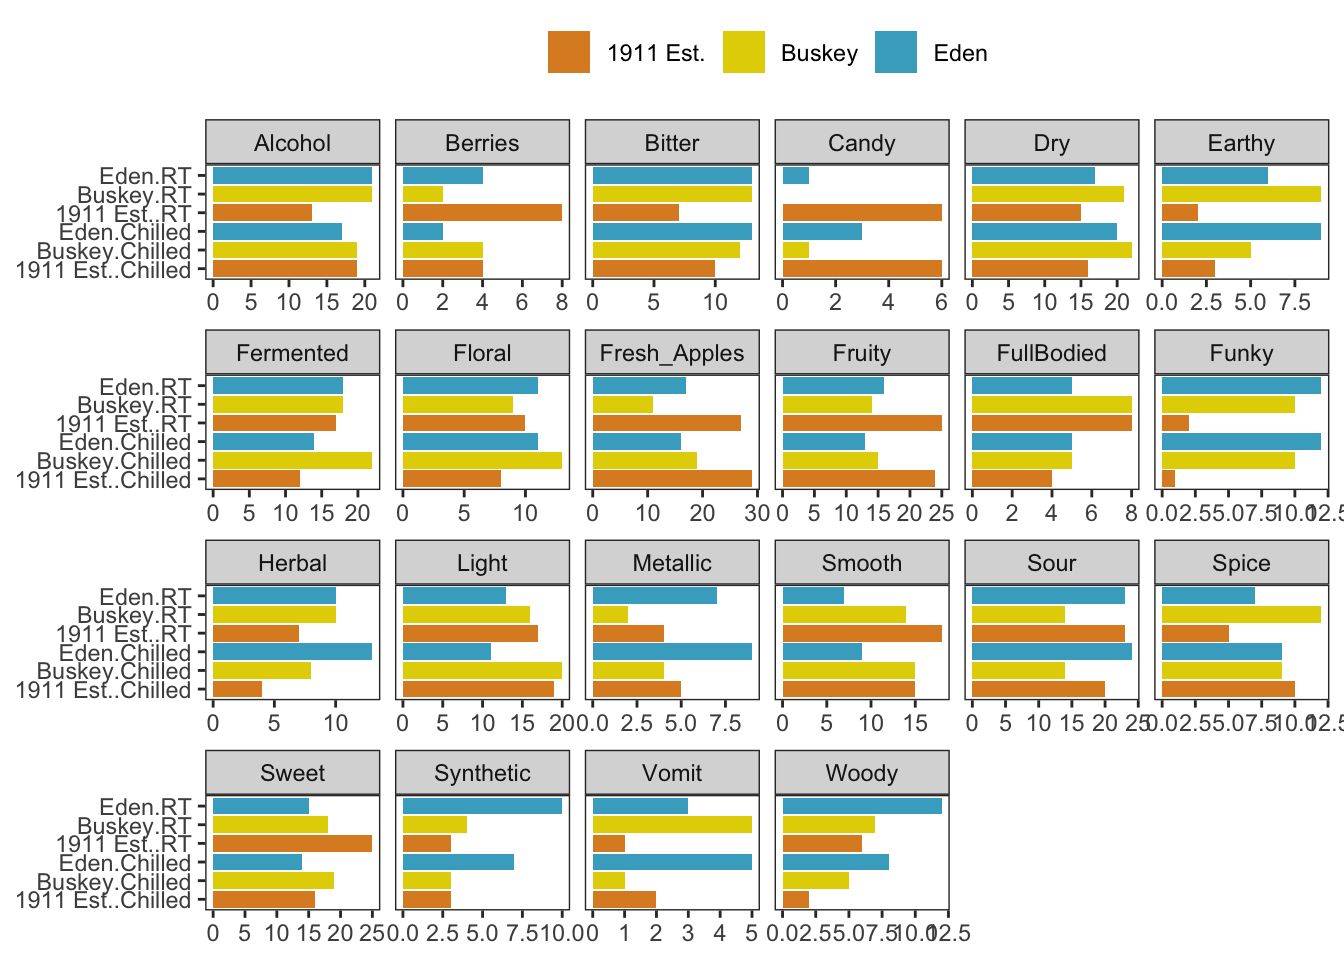
\includegraphics{04-ggplot2-extensions_files/figure-latex/faceted plots with different x-axes-1} \end{center}

Not that we'd argue you \emph{should} here. Also, take note that the \texttt{x} in \texttt{free\_x} refers to the horizontal axis in the final plot, \emph{after} the \texttt{coord\_flip()}, and \emph{not} the \texttt{x} aesthetic we set in the \texttt{ggplot()} call.

But if you have different plot types entirely (different data sources, different \texttt{geom\_()}s, or different categorical axes) that you want to place side-by-side, say a loading plot and the product map resulting from a PCA or MFA, you're going to need something to paste together multiple \texttt{ggplot\_()}s.

The easiest way to do this is using \texttt{patchwork}, which will work on ggplots you've made yourself \emph{or} with ones made by packages like \texttt{FactoMineR}. \emph{When you have \texttt{patchwork} loaded}, the \texttt{+} operator will put two plots side-by-side:

\begin{Shaded}
\begin{Highlighting}[]
\FunctionTok{library}\NormalTok{(patchwork)}
\FunctionTok{plot}\NormalTok{(berry\_mfa\_res, }\AttributeTok{choix =} \StringTok{"var"}\NormalTok{) }\SpecialCharTok{+} \FunctionTok{plot}\NormalTok{(berry\_mfa\_res, }\AttributeTok{partial =} \StringTok{"all"}\NormalTok{)}
\end{Highlighting}
\end{Shaded}

\begin{center}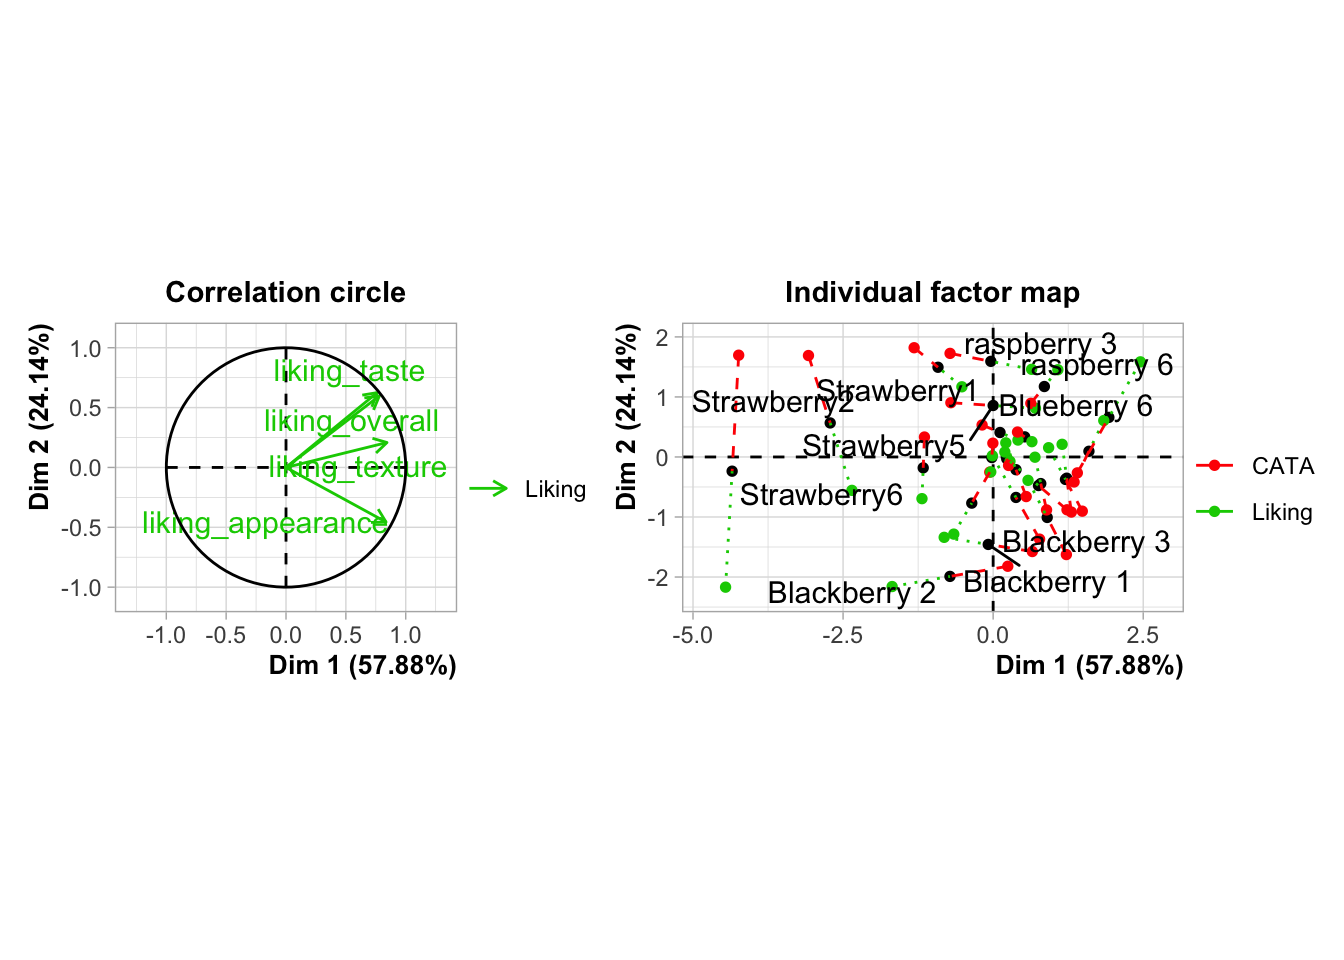
\includegraphics{04-ggplot2-extensions_files/figure-latex/combining plots with patchwork-1} \end{center}

And the \texttt{/} operator will arrange two plots vertically:

\begin{Shaded}
\begin{Highlighting}[]
\FunctionTok{plot}\NormalTok{(berry\_mfa\_res, }\AttributeTok{choix =} \StringTok{"var"}\NormalTok{) }\SpecialCharTok{/} \FunctionTok{plot}\NormalTok{(berry\_mfa\_res, }\AttributeTok{partial =} \StringTok{"all"}\NormalTok{)}
\end{Highlighting}
\end{Shaded}

\begin{center}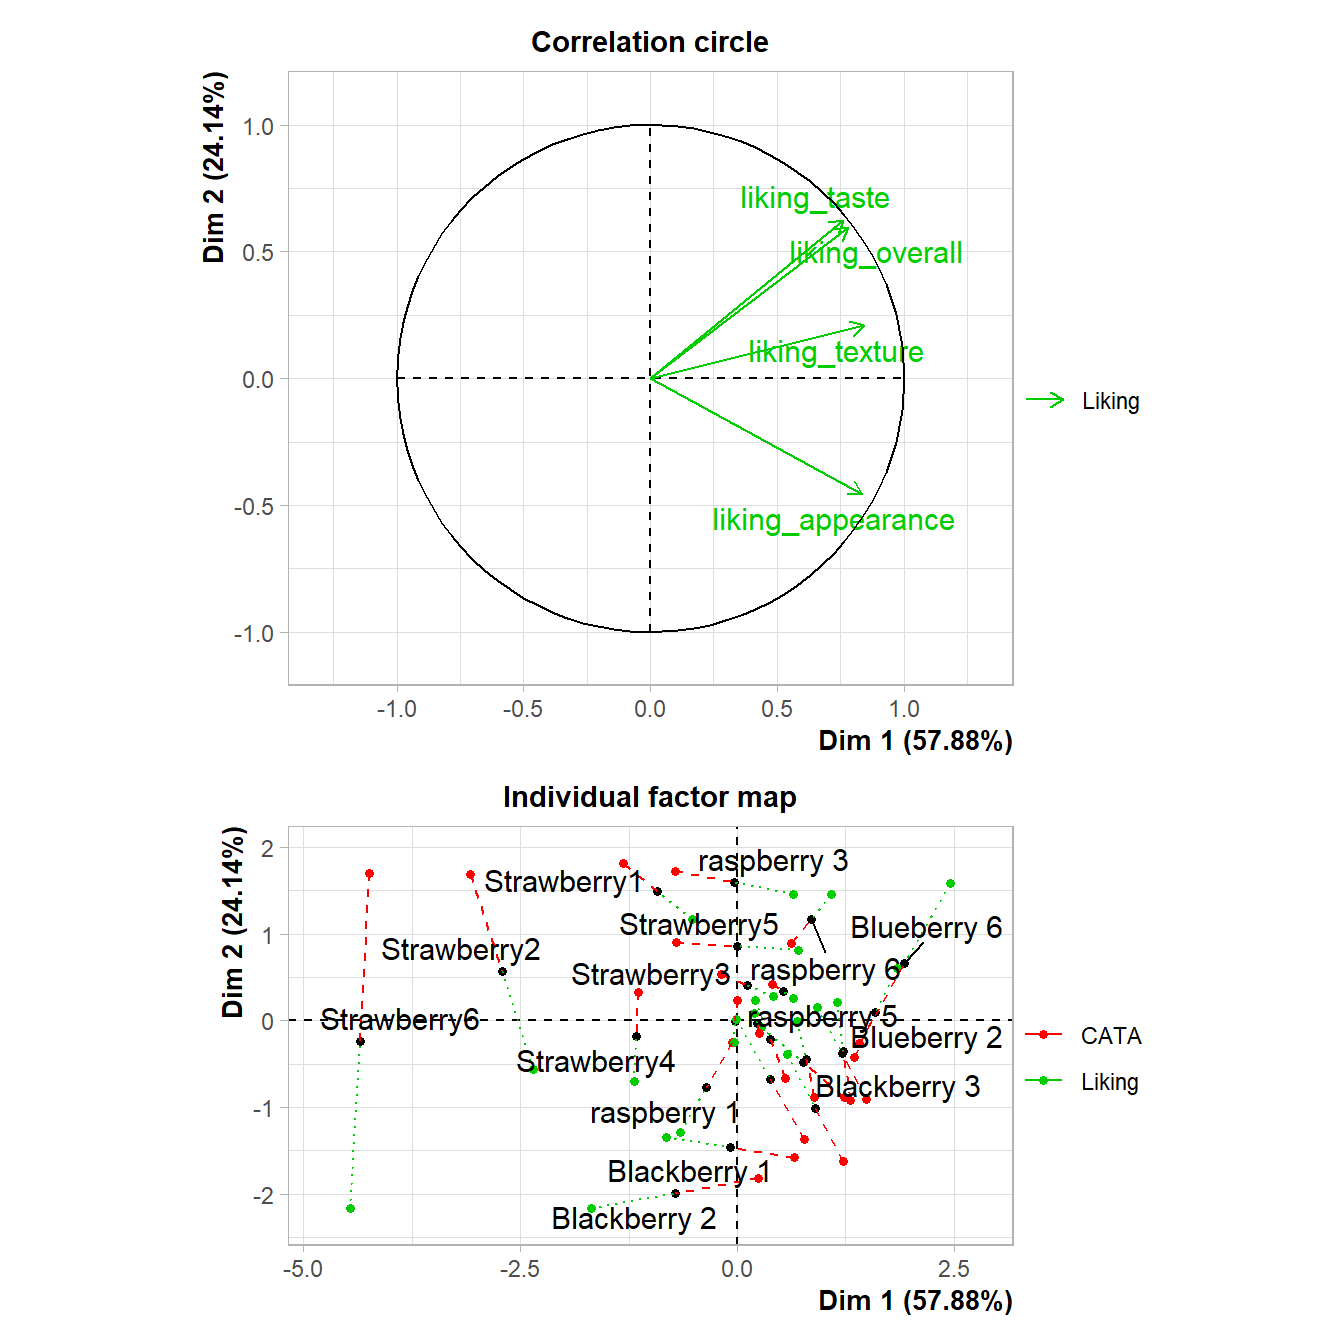
\includegraphics{04-ggplot2-extensions_files/figure-latex/arranging plots vertically with patchwork-1} \end{center}

The advantage of doing this with a package like \texttt{patchwork}, rather than saving separate images, is that it aligns all of the plot areas precisely and that they will more easily move or rearrange certain plot elements like legends and axis labels.

\begin{Shaded}
\begin{Highlighting}[]
\FunctionTok{plot}\NormalTok{(berry\_mfa\_res, }\AttributeTok{choix =} \StringTok{"var"}\NormalTok{) }\SpecialCharTok{+} \FunctionTok{plot}\NormalTok{(berry\_mfa\_res, }\AttributeTok{partial =} \StringTok{"all"}\NormalTok{) }\SpecialCharTok{+}
  \FunctionTok{plot\_layout}\NormalTok{(}\AttributeTok{guides =} \StringTok{"collect"}\NormalTok{) }\SpecialCharTok{\&}
  \FunctionTok{theme}\NormalTok{(}\AttributeTok{plot.title =} \FunctionTok{element\_blank}\NormalTok{(),}
        \AttributeTok{legend.position =} \StringTok{"bottom"}\NormalTok{)}
\end{Highlighting}
\end{Shaded}

\begin{center}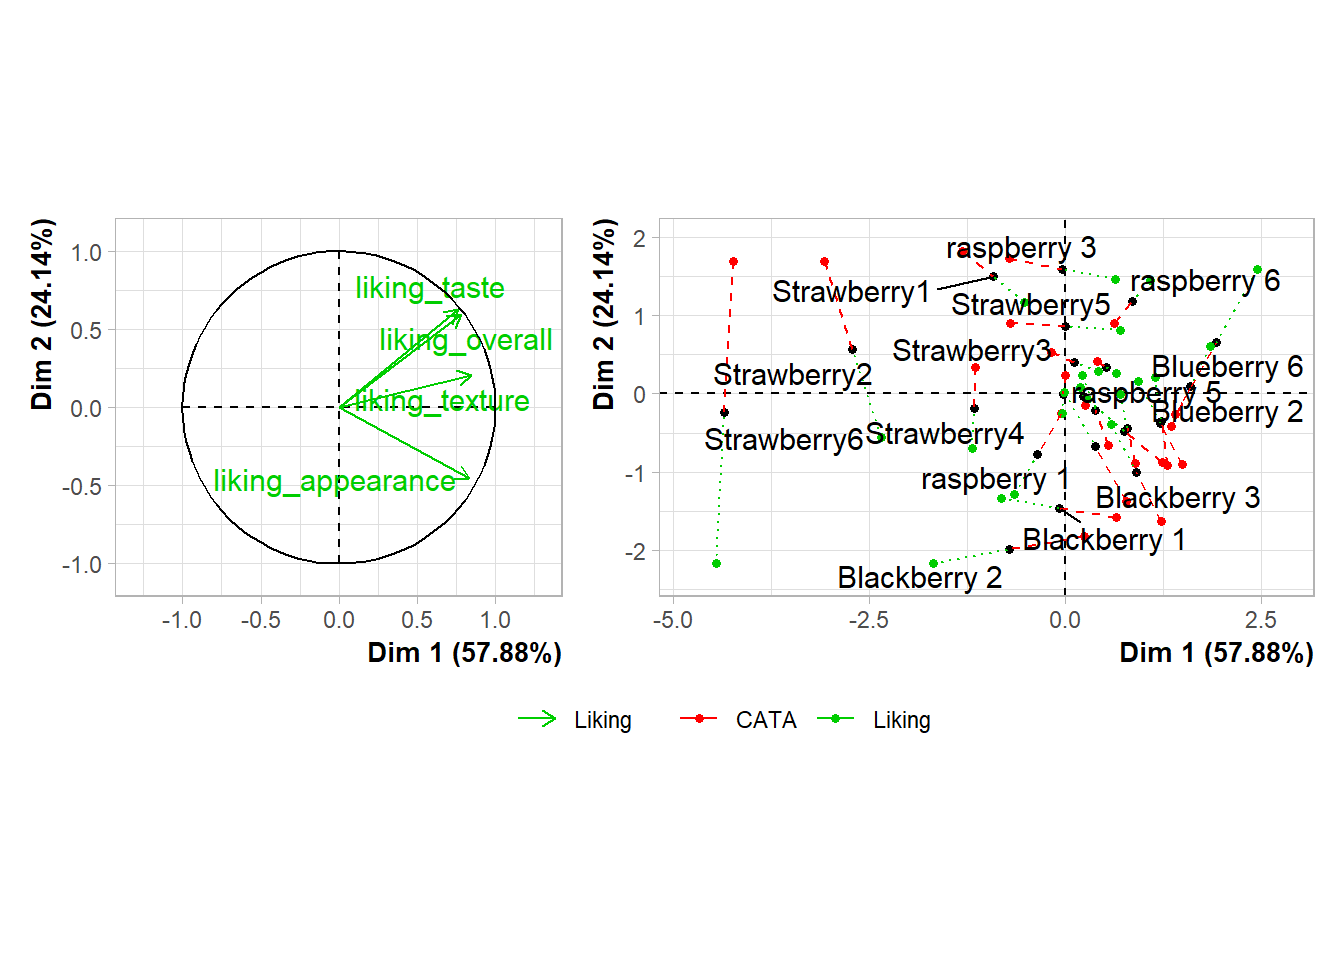
\includegraphics{04-ggplot2-extensions_files/figure-latex/collecting legends at the bottom of a patchwork ensemble-1} \end{center}

The \texttt{\&} operator lets you add elements like themes or annotations to all of the plots you've combined together. \texttt{plot\_layout()} is a \texttt{patchwork} function that lets you set relative plot sizes, decide how to arrange more than 2 plots, and move legends:

\begin{Shaded}
\begin{Highlighting}[]
\FunctionTok{plot}\NormalTok{(berry\_mfa\_res, }\AttributeTok{partial =} \StringTok{"all"}\NormalTok{) }\SpecialCharTok{+}
\NormalTok{  (}\FunctionTok{plot}\NormalTok{(berry\_mfa\_res, }\AttributeTok{choix =} \StringTok{"var"}\NormalTok{) }\SpecialCharTok{+}
  \FunctionTok{plot}\NormalTok{(berry\_mfa\_res, }\AttributeTok{choix =} \StringTok{"freq"}\NormalTok{, }\AttributeTok{invisible =} \StringTok{"ind"}\NormalTok{)) }\SpecialCharTok{+}
  \FunctionTok{plot\_layout}\NormalTok{(}\AttributeTok{guides =} \StringTok{"collect"}\NormalTok{, }\AttributeTok{ncol =} \DecValTok{1}\NormalTok{, }\AttributeTok{widths =} \DecValTok{2}\NormalTok{) }\SpecialCharTok{\&}
  \FunctionTok{theme}\NormalTok{(}\AttributeTok{plot.title =} \FunctionTok{element\_blank}\NormalTok{(),}
        \AttributeTok{axis.title =} \FunctionTok{element\_blank}\NormalTok{(),}
        \AttributeTok{legend.position =} \StringTok{"bottom"}\NormalTok{)}
\end{Highlighting}
\end{Shaded}

\begin{center}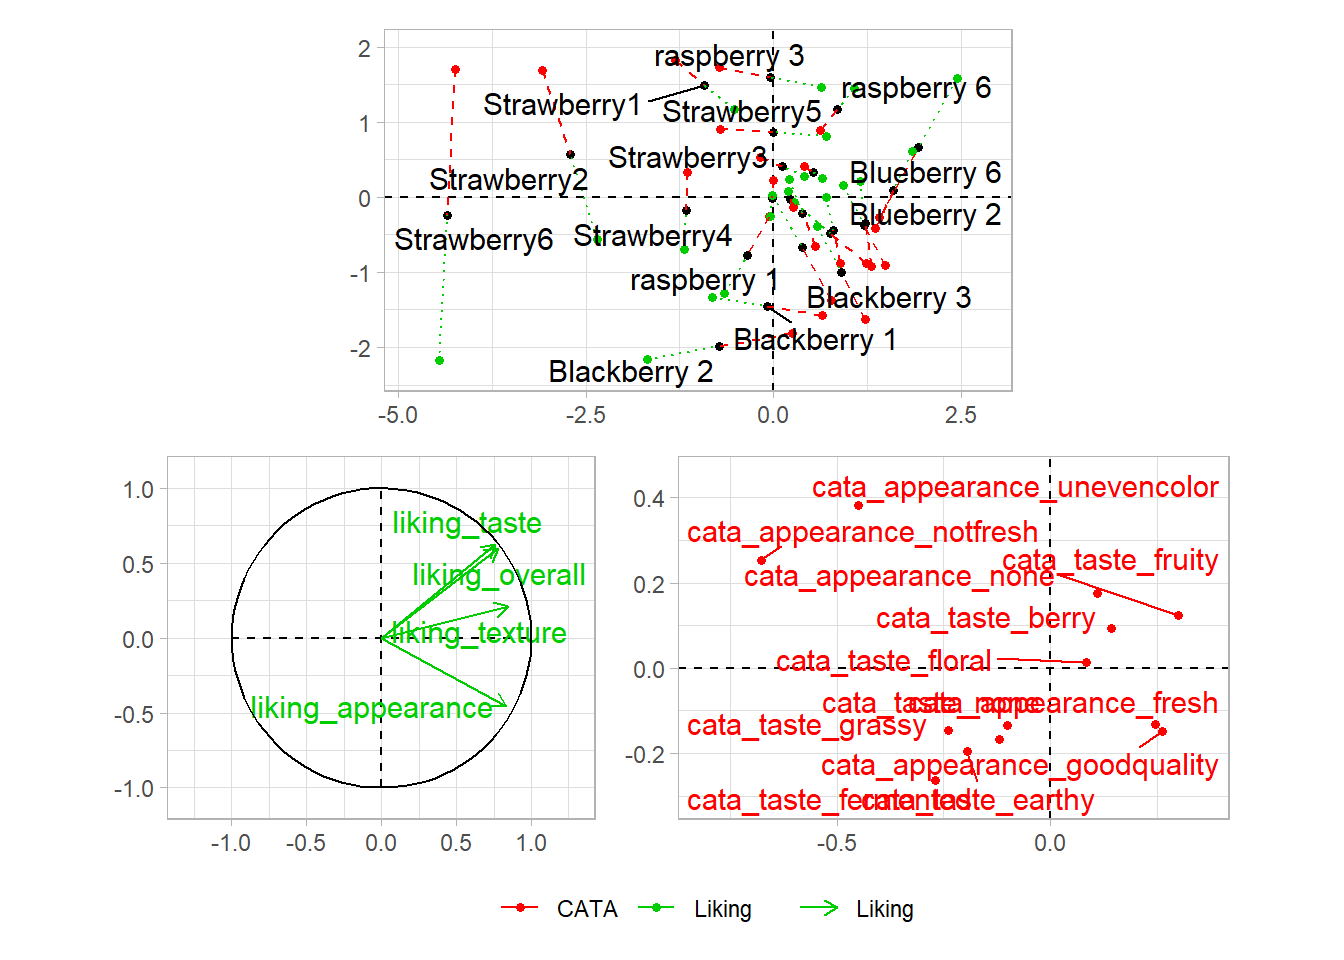
\includegraphics{04-ggplot2-extensions_files/figure-latex/more complex patchwork layout-1} \end{center}

If you want to put images anywhere on a visualization, you're struggling to make a complex arrangement with \texttt{patchwork}, or you have an \texttt{R} \texttt{list} structure containing multiple plots (say, the result of a \texttt{for} loop, \texttt{*apply()}, or \texttt{nest()} call), then \texttt{cowplot} is another option:

\begin{Shaded}
\begin{Highlighting}[]
\NormalTok{berry\_mfa\_res}\SpecialCharTok{$}\NormalTok{separate.analyses }\SpecialCharTok{\%\textgreater{}\%}
  \FunctionTok{lapply}\NormalTok{(}\ControlFlowTok{function}\NormalTok{(x) \{}
\NormalTok{    x}\SpecialCharTok{$}\NormalTok{ind}\SpecialCharTok{$}\NormalTok{coord }\SpecialCharTok{\%\textgreater{}\%}
      \FunctionTok{as\_tibble}\NormalTok{(}\AttributeTok{rownames =} \StringTok{"Berry"}\NormalTok{) }\SpecialCharTok{\%\textgreater{}\%}
      \FunctionTok{ggplot}\NormalTok{(}\FunctionTok{aes}\NormalTok{(}\AttributeTok{x =}\NormalTok{ Dim}\FloatTok{.1}\NormalTok{, }\AttributeTok{y =}\NormalTok{ Dim}\FloatTok{.2}\NormalTok{)) }\SpecialCharTok{+}
      \FunctionTok{geom\_point}\NormalTok{()}
\NormalTok{  \}) }\SpecialCharTok{\%\textgreater{}\%}
\NormalTok{  cowplot}\SpecialCharTok{::}\FunctionTok{plot\_grid}\NormalTok{(}\AttributeTok{plotlist =}\NormalTok{ ., }\AttributeTok{labels =} \FunctionTok{names}\NormalTok{(.))}
\end{Highlighting}
\end{Shaded}

\begin{center}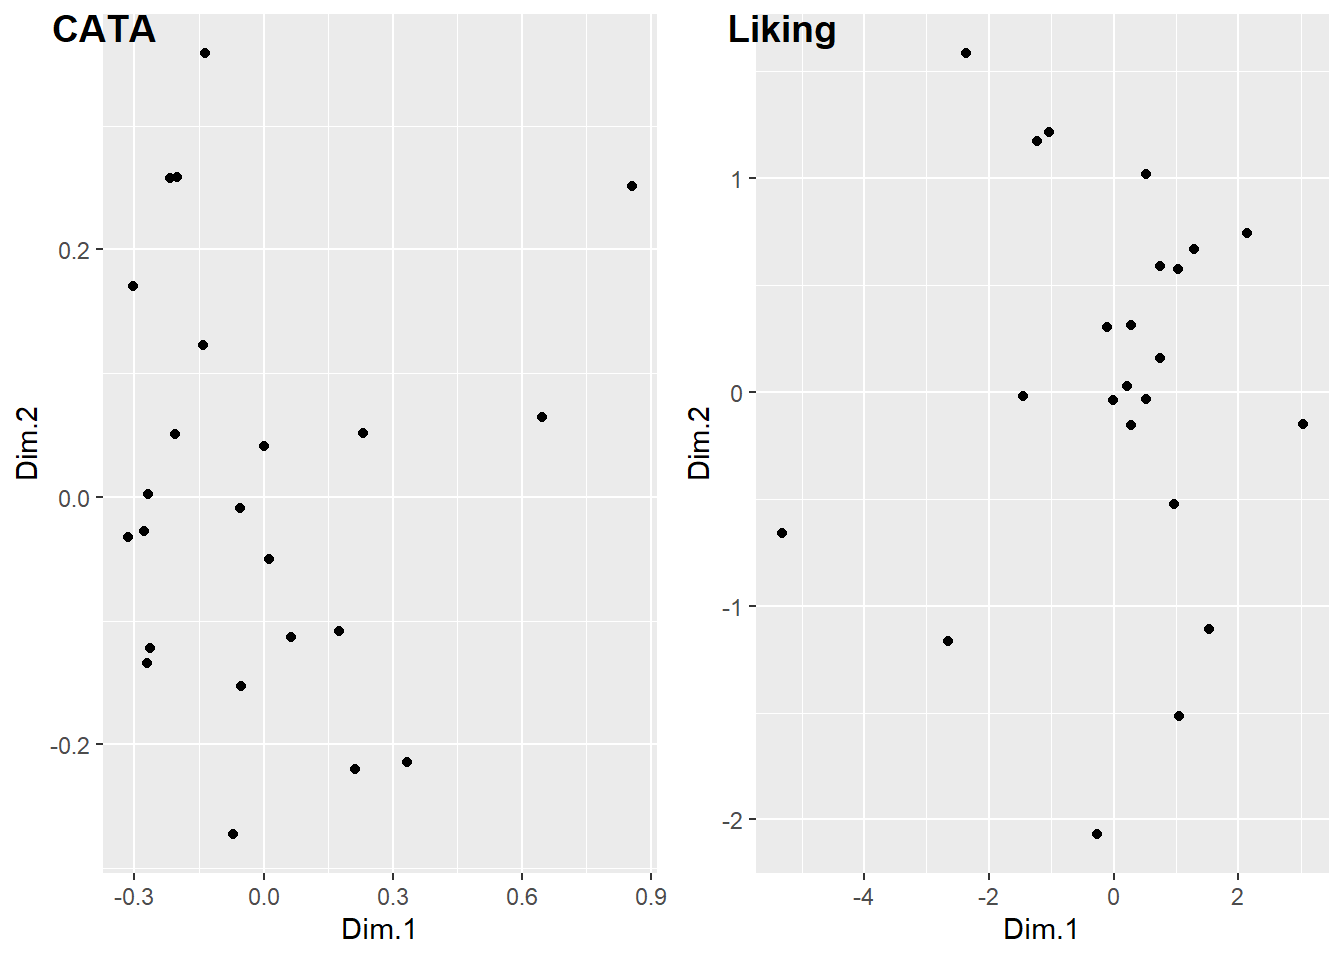
\includegraphics{04-ggplot2-extensions_files/figure-latex/plotting a list-1} \end{center}

\begin{Shaded}
\begin{Highlighting}[]
\CommentTok{\#You can also pipe your list into patchwork::wrap\_plots()}
\CommentTok{\#if you have the latest version of patchwork.}
\CommentTok{\#It\textquotesingle{}s a fairly new package, so it gains big new features very often.}
\end{Highlighting}
\end{Shaded}

Both of these packages can also add letters and other labels to each plot:

\begin{Shaded}
\begin{Highlighting}[]
\FunctionTok{plot}\NormalTok{(berry\_mfa\_res, }\AttributeTok{choix =} \StringTok{"var"}\NormalTok{) }\SpecialCharTok{+} \FunctionTok{plot}\NormalTok{(berry\_mfa\_res, }\AttributeTok{partial =} \StringTok{"all"}\NormalTok{) }\SpecialCharTok{+}
  \FunctionTok{plot\_layout}\NormalTok{(}\AttributeTok{guides =} \StringTok{"collect"}\NormalTok{) }\SpecialCharTok{+}
  \FunctionTok{plot\_annotation}\NormalTok{(}\AttributeTok{tag\_levels =} \StringTok{\textquotesingle{}A\textquotesingle{}}\NormalTok{) }\SpecialCharTok{\&}
  \FunctionTok{theme}\NormalTok{(}\AttributeTok{plot.title =} \FunctionTok{element\_blank}\NormalTok{(),}
        \AttributeTok{legend.position =} \StringTok{"bottom"}\NormalTok{)}
\end{Highlighting}
\end{Shaded}

\begin{center}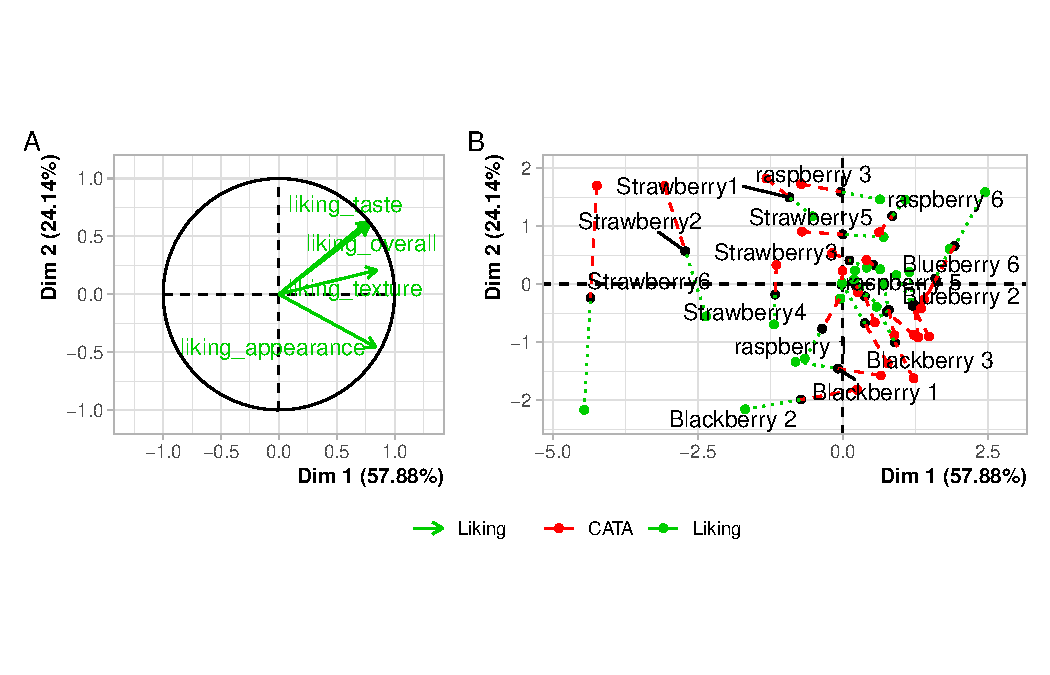
\includegraphics{04-ggplot2-extensions_files/figure-latex/labeling plots-1} \end{center}

\begin{Shaded}
\begin{Highlighting}[]
\NormalTok{cowplot}\SpecialCharTok{::}\FunctionTok{plot\_grid}\NormalTok{(}\FunctionTok{plot}\NormalTok{(berry\_mfa\_res, }\AttributeTok{choix =} \StringTok{"var"}\NormalTok{),}
                   \FunctionTok{plot}\NormalTok{(berry\_mfa\_res, }\AttributeTok{partial =} \StringTok{"all"}\NormalTok{),}
                   \AttributeTok{labels =} \StringTok{"AUTO"}\NormalTok{)}
\end{Highlighting}
\end{Shaded}

\begin{center}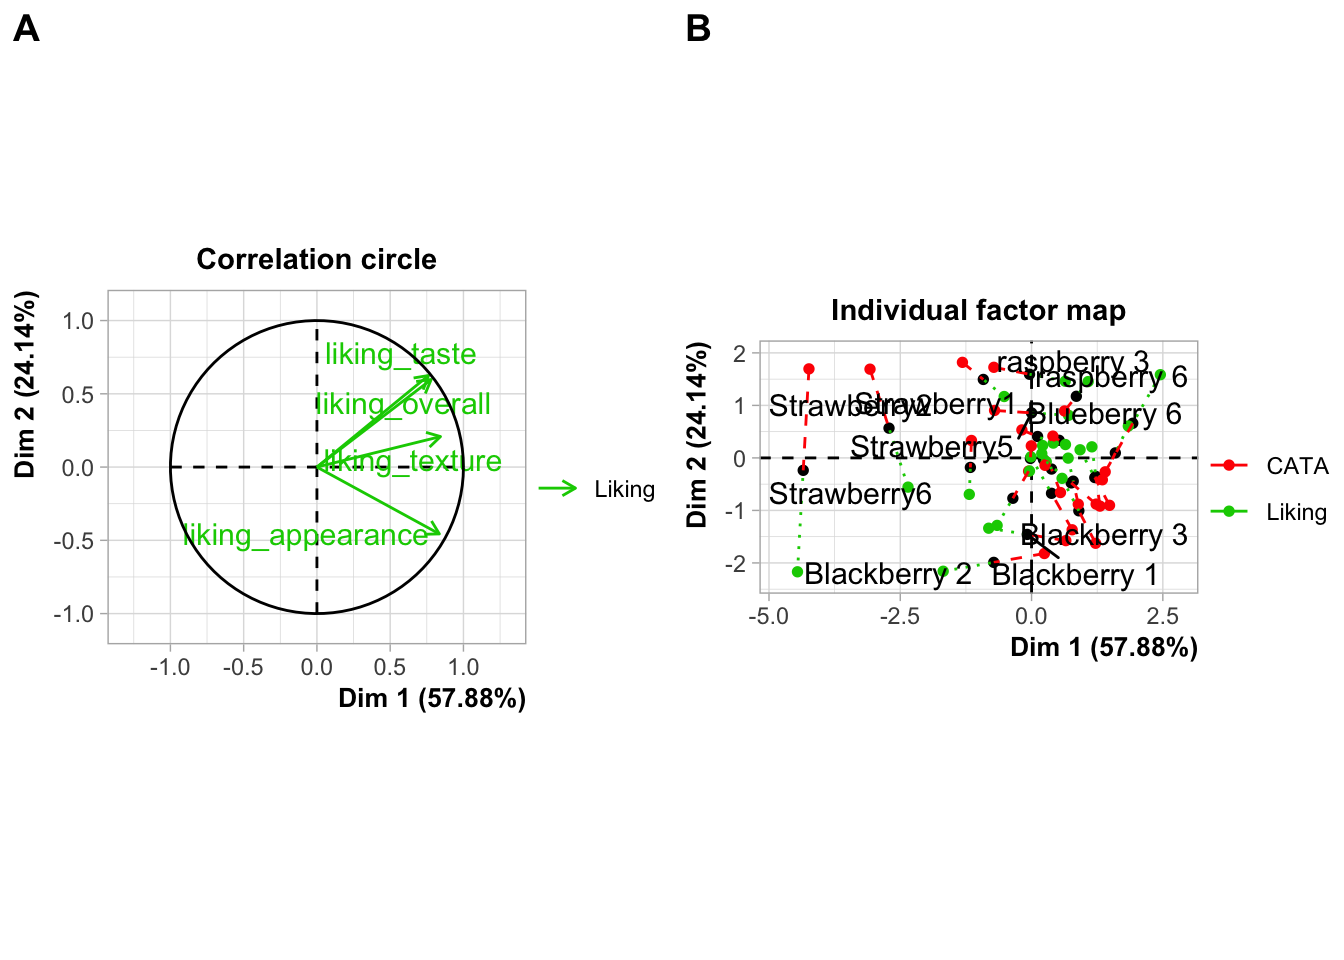
\includegraphics{04-ggplot2-extensions_files/figure-latex/labeling plots-2} \end{center}

\begin{Shaded}
\begin{Highlighting}[]
\CommentTok{\#Cowplot doesn\textquotesingle{}t have a way to combine or move legends.}
\CommentTok{\#You\textquotesingle{}d have to move the legends *before* using plot\_grid()}
\end{Highlighting}
\end{Shaded}

If you need to move or realign the labels so they're not overlapping anything, in \texttt{patchwork} you can add \texttt{theme(plot.tag.position\ =\ c(X,\ Y))} to individual plots with \texttt{+} or to the whole grouping of plots with \texttt{\&}. The \texttt{cowplot::plot\_grid()} function has arguments \texttt{labels\_x} and \texttt{labels\_y}, which let you adjust the distance from the bottom left hand corner of the figure.

\begin{Shaded}
\begin{Highlighting}[]
\FunctionTok{plot}\NormalTok{(berry\_mfa\_res, }\AttributeTok{choix =} \StringTok{"var"}\NormalTok{) }\SpecialCharTok{+} \FunctionTok{theme}\NormalTok{(}\AttributeTok{plot.tag.position =} \FunctionTok{c}\NormalTok{(}\FloatTok{0.2}\NormalTok{, }\FloatTok{0.95}\NormalTok{)) }\SpecialCharTok{+}
  \FunctionTok{plot}\NormalTok{(berry\_mfa\_res, }\AttributeTok{partial =} \StringTok{"all"}\NormalTok{) }\SpecialCharTok{+} \FunctionTok{theme}\NormalTok{(}\AttributeTok{plot.tag.position =} \FunctionTok{c}\NormalTok{(}\FloatTok{0.12}\NormalTok{, }\FloatTok{0.95}\NormalTok{)) }\SpecialCharTok{+}
  \FunctionTok{plot\_layout}\NormalTok{(}\AttributeTok{guides =} \StringTok{"collect"}\NormalTok{) }\SpecialCharTok{+}
  \FunctionTok{plot\_annotation}\NormalTok{(}\AttributeTok{tag\_levels =} \StringTok{\textquotesingle{}A\textquotesingle{}}\NormalTok{) }\SpecialCharTok{\&}
  \FunctionTok{theme}\NormalTok{(}\AttributeTok{plot.title =} \FunctionTok{element\_blank}\NormalTok{(),}
        \AttributeTok{legend.position =} \StringTok{"bottom"}\NormalTok{)}
\end{Highlighting}
\end{Shaded}

\begin{center}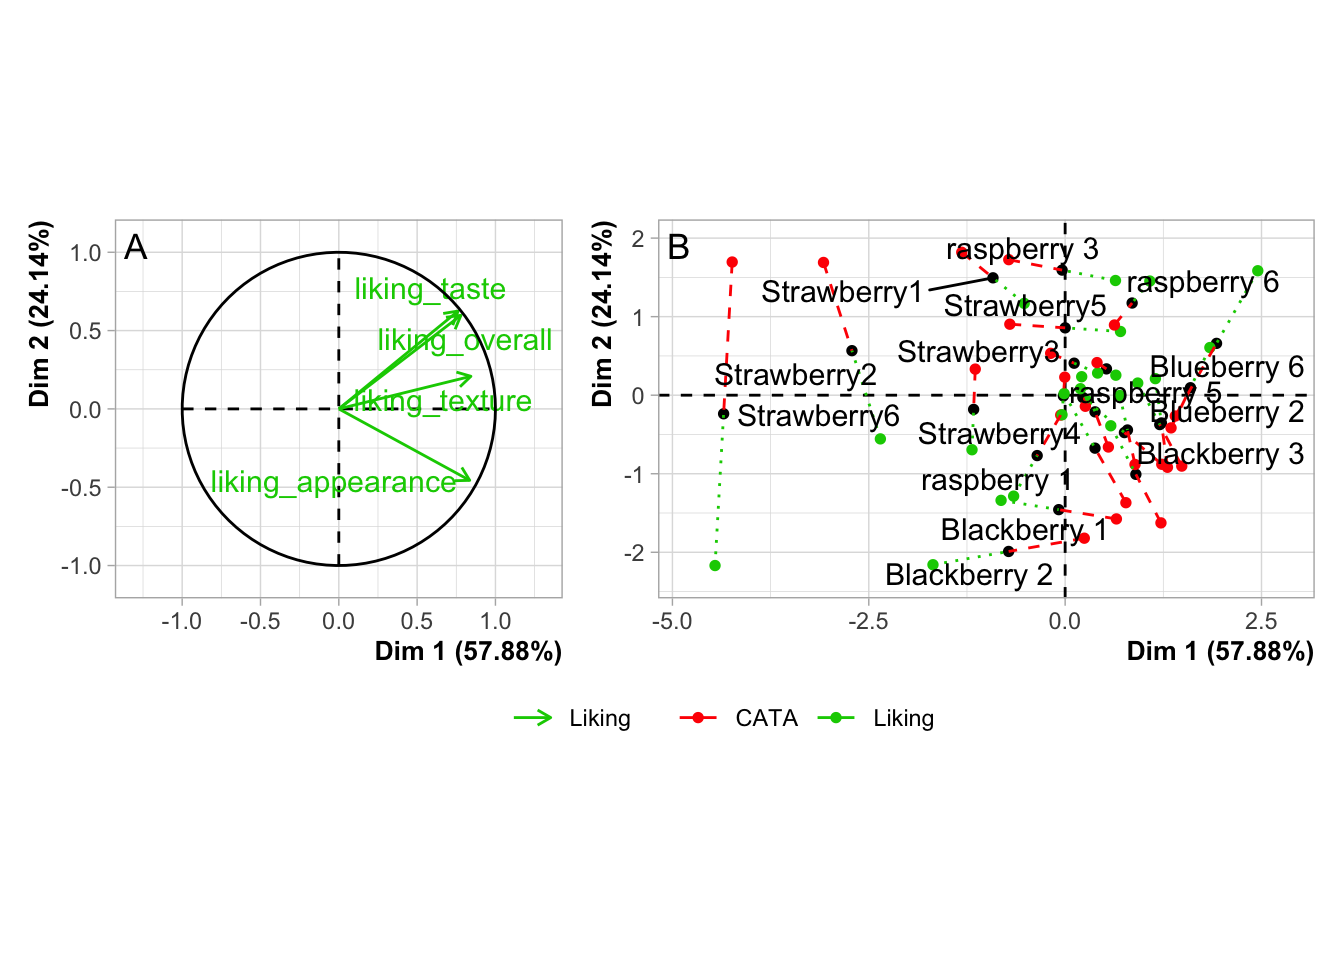
\includegraphics{04-ggplot2-extensions_files/figure-latex/moving plot labels-1} \end{center}

\begin{Shaded}
\begin{Highlighting}[]
\NormalTok{cowplot}\SpecialCharTok{::}\FunctionTok{plot\_grid}\NormalTok{(}\FunctionTok{plot}\NormalTok{(berry\_mfa\_res, }\AttributeTok{choix =} \StringTok{"var"}\NormalTok{),}
                   \FunctionTok{plot}\NormalTok{(berry\_mfa\_res, }\AttributeTok{partial =} \StringTok{"all"}\NormalTok{),}
                   \AttributeTok{labels =} \StringTok{"AUTO"}\NormalTok{,}
                   \AttributeTok{label\_y =} \FloatTok{0.8}\NormalTok{)}
\end{Highlighting}
\end{Shaded}

\begin{center}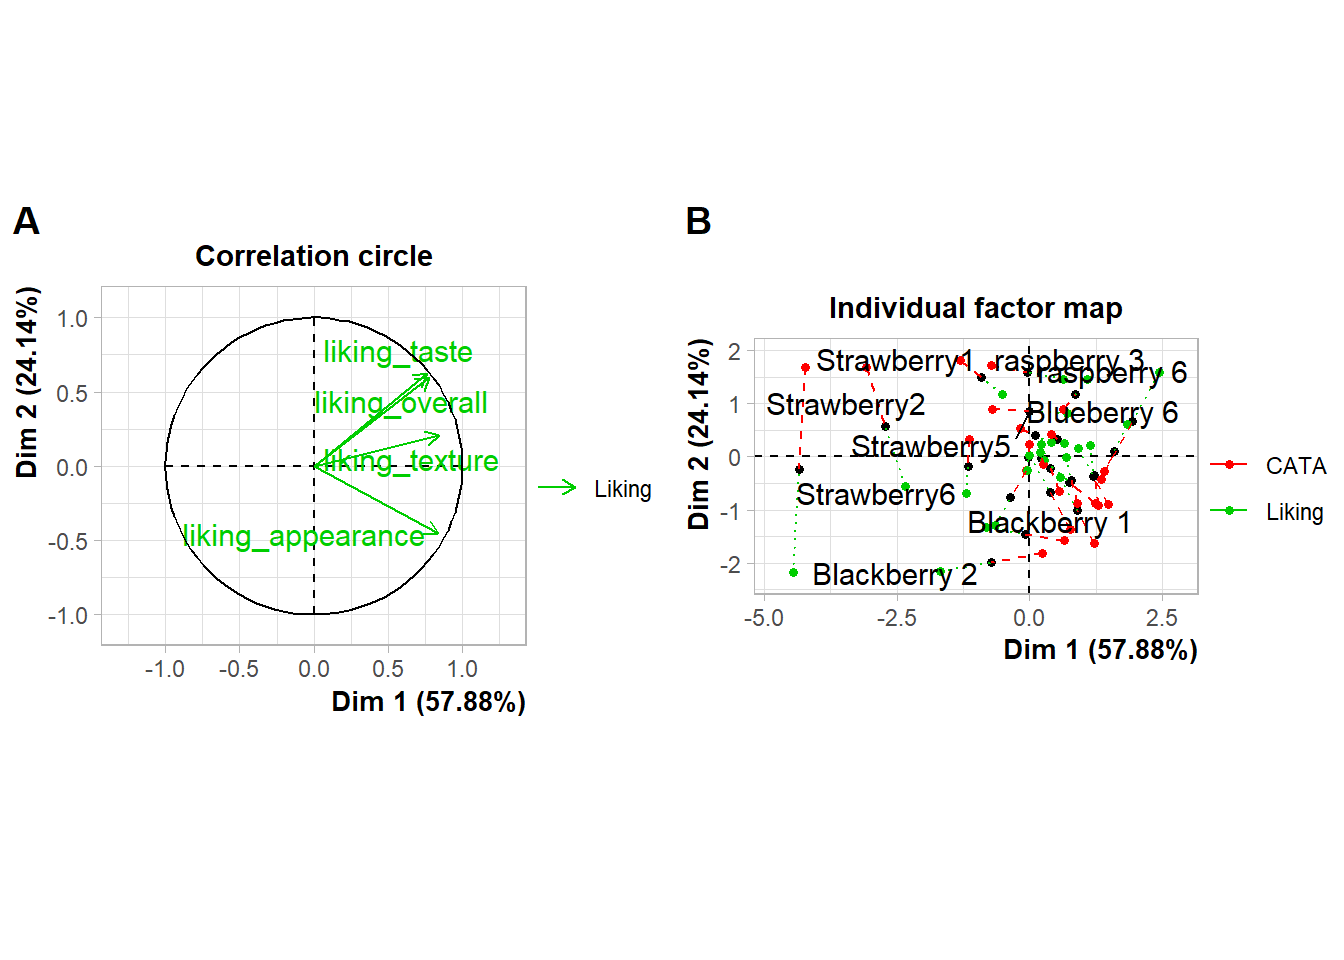
\includegraphics{04-ggplot2-extensions_files/figure-latex/moving plot labels-2} \end{center}

You can also use any image editing, publishing, or graphics software to manually combine, arrange, and label plots, but if you need to make changes to a plot later then doing your layout \emph{in \texttt{R}} will mean you just have to run the lightly-updated code again to re-export a fully formatted multi-part figure, even if the plot dimensions change.

\hypertarget{finding-new-packages}{%
\section{Finding New Packages}\label{finding-new-packages}}

This isn't all the functionality of any of these packages, and these aren't the only packages that add new features to \texttt{ggplot2}.

If you're trying to figure out how to create a type of plot you've never made before, we'd recommend:

\begin{enumerate}
\def\labelenumi{\arabic{enumi}.}
\tightlist
\item
  Ask yourself what variables are represented by the x and y axes, the shapes, the line types, or the colors. Think about whether you can build the plot from smaller components. Is it a grid of scatterplots with colored contour regions? How much of the plot is just points, lines, or rectangles with fancy formatting? You can do \textbf{a lot} with just \texttt{ggplot2}!
\item
  See if any of the packages in \href{https://exts.ggplot2.tidyverse.org/gallery/}{the list of registered ggplot extensions} have a plot similar to yours. These packages tend to have very thorough and visual documentation.
\item
  If it's a sensory-specific plot, \href{https://jlahne.github.io/r-opus-v2/index.html}{check out the \texttt{R} Opus v2}. Almost all of the plots only use \texttt{ggplot2}, \texttt{patchwork}, and \texttt{ggrepel}.
\item
  Use a web search with the kind of plot you want to make and the keyword ``ggplot2'' to find tutorials or discussions with example code. Results from \href{https://stackoverflow.com/questions/tagged/ggplot2}{Stack Overflow}, \href{https://www.data-to-viz.com/}{Data to Viz}, or \href{https://r-graph-gallery.com/index.html}{\texttt{R} Graph Gallery} are all likely to have good explanations and useful examples, while anything with ``(\# examples)'' in the article name is likely to be very basic material with good SEO.
\end{enumerate}

Keep in mind that keywords primarily used in sensory science, say ``preference map'' or ``penalty analysis'', are unlikely to yield examples in \texttt{ggplot2} with extensive results. In my own process of troubleshooting and double-checking for this workshop, I've found some helpful examples by searching ``add density contours to 2d scatterplot ggplot'' or ``ordered bar plot positive and negative ggplot''.

Package documentation might come up while you're looking, but the examples are often very abstract and simple, and they're often structured around names of functions rather than concepts, so it's often faster to see some examples of real plots that other people (who aren't writing an entire \texttt{R} package) wanted to make and then looking up the functions they used to do so.

Now, with the rest of the time we have left, I'm going to try and show off how I do some of the most common cleaning-up when it's time to actually present or publish.

\hypertarget{fine-tuning-publication-quality-ggplots}{%
\chapter{Fine-Tuning Publication-Quality ggplots}\label{fine-tuning-publication-quality-ggplots}}

The plots we've been making so far are fairly straightforward demonstrations. At the very end of Chapter 3, we briefly showed you the code and results for this plot:

\begin{Shaded}
\begin{Highlighting}[]
\NormalTok{berry\_penalty\_analysis\_data }\SpecialCharTok{\%\textgreater{}\%}
  \FunctionTok{select}\NormalTok{(}\SpecialCharTok{{-}}\NormalTok{count) }\SpecialCharTok{\%\textgreater{}\%}
  \FunctionTok{pivot\_wider}\NormalTok{(}\AttributeTok{names\_from =}\NormalTok{ checked,}
              \AttributeTok{values\_from =}\NormalTok{ penalty\_lift,}
              \AttributeTok{names\_prefix =} \StringTok{"checked\_"}\NormalTok{) }\SpecialCharTok{\%\textgreater{}\%}
  \FunctionTok{separate}\NormalTok{(cata\_variable, }
           \AttributeTok{into =} \FunctionTok{c}\NormalTok{(}\StringTok{"mode"}\NormalTok{, }\StringTok{"variable"}\NormalTok{), }
           \AttributeTok{sep =} \StringTok{"\_"}\NormalTok{) }\SpecialCharTok{\%\textgreater{}\%}
  \FunctionTok{mutate}\NormalTok{(}\AttributeTok{penalty\_lift =}\NormalTok{ checked\_1 }\SpecialCharTok{{-}}\NormalTok{ checked\_0,}
         \AttributeTok{mode =} \FunctionTok{case\_when}\NormalTok{(mode }\SpecialCharTok{==} \StringTok{"taste"} \SpecialCharTok{\textasciitilde{}} \StringTok{"(T)"}\NormalTok{,}
\NormalTok{                          mode }\SpecialCharTok{==} \StringTok{"appearance"} \SpecialCharTok{\textasciitilde{}} \StringTok{"(A)"}\NormalTok{,}
\NormalTok{                          mode }\SpecialCharTok{==} \StringTok{"appearane"} \SpecialCharTok{\textasciitilde{}} \StringTok{"(A)"}\NormalTok{)) }\SpecialCharTok{\%\textgreater{}\%}
  \FunctionTok{unite}\NormalTok{(variable, mode, }\AttributeTok{col =} \StringTok{"cata\_variable"}\NormalTok{, }\AttributeTok{sep =} \StringTok{" "}\NormalTok{) }\SpecialCharTok{\%\textgreater{}\%}
  \FunctionTok{mutate}\NormalTok{(}\AttributeTok{cata\_variable =}\NormalTok{ tidytext}\SpecialCharTok{::}\FunctionTok{reorder\_within}\NormalTok{(}\AttributeTok{x =}\NormalTok{ cata\_variable,}
                                                  \AttributeTok{by =}\NormalTok{ penalty\_lift,}
                                                  \AttributeTok{within =}\NormalTok{ berry)) }\SpecialCharTok{\%\textgreater{}\%}
  \FunctionTok{ggplot}\NormalTok{(}\AttributeTok{mapping =} \FunctionTok{aes}\NormalTok{(}\AttributeTok{x =}\NormalTok{ cata\_variable, }\AttributeTok{y =}\NormalTok{ penalty\_lift)) }\SpecialCharTok{+}
  \FunctionTok{geom\_col}\NormalTok{(}\FunctionTok{aes}\NormalTok{(}\AttributeTok{fill =}\NormalTok{ penalty\_lift), }\AttributeTok{color =} \StringTok{"white"}\NormalTok{, }\AttributeTok{show.legend =} \ConstantTok{FALSE}\NormalTok{) }\SpecialCharTok{+} 
  \FunctionTok{facet\_wrap}\NormalTok{(}\SpecialCharTok{\textasciitilde{}}\NormalTok{berry, }\AttributeTok{scales =} \StringTok{"free"}\NormalTok{, }\AttributeTok{nrow =} \DecValTok{1}\NormalTok{) }\SpecialCharTok{+} 
\NormalTok{  tidytext}\SpecialCharTok{::}\FunctionTok{scale\_x\_reordered}\NormalTok{() }\SpecialCharTok{+} 
  \FunctionTok{coord\_flip}\NormalTok{() }\SpecialCharTok{+} 
  \FunctionTok{theme\_classic}\NormalTok{() }\SpecialCharTok{+} 
  \FunctionTok{scale\_fill\_gradient}\NormalTok{(}\AttributeTok{low =} \StringTok{"tan"}\NormalTok{, }\AttributeTok{high =} \StringTok{"darkgreen"}\NormalTok{) }\SpecialCharTok{+} 
  \FunctionTok{labs}\NormalTok{(}\AttributeTok{x =} \ConstantTok{NULL}\NormalTok{, }\AttributeTok{y =} \ConstantTok{NULL}\NormalTok{,}
       \AttributeTok{title =} \StringTok{"Penalty / Lift Analysis"}\NormalTok{,}
       \AttributeTok{subtitle =} \StringTok{"displays the mean difference (within berries) for when a CATA variable is checked}\SpecialCharTok{\textbackslash{}n}\StringTok{or un{-}checked"}\NormalTok{) }\OtherTok{{-}\textgreater{}}
\NormalTok{  goal\_plot}

\NormalTok{goal\_plot}
\end{Highlighting}
\end{Shaded}

\begin{center}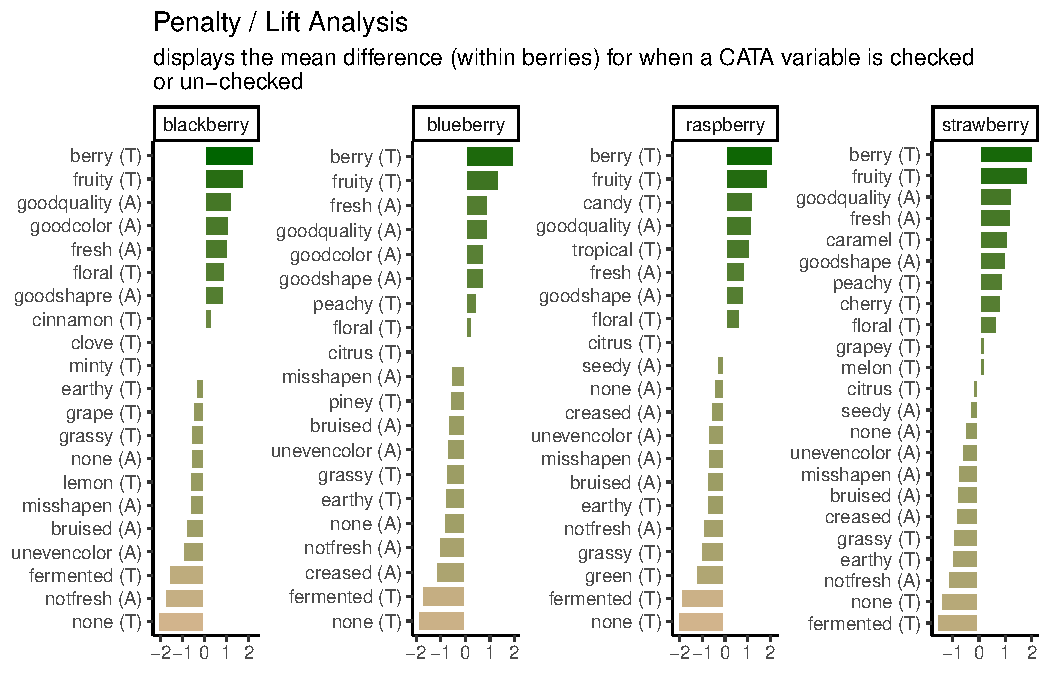
\includegraphics{05-finetuning-ggplot_files/figure-latex/penalty analysis example-1} \end{center}

Which uses some tricks from the \texttt{stringr} and \texttt{tidytext} packages in order to give us easy-to-read labels. Using the existing column names and variable-codes in our original data to make a first draft of a plot, it would've looked more like this:

\begin{Shaded}
\begin{Highlighting}[]
\NormalTok{berry\_penalty\_analysis\_data }\SpecialCharTok{\%\textgreater{}\%}
  \FunctionTok{select}\NormalTok{(}\SpecialCharTok{{-}}\NormalTok{count) }\SpecialCharTok{\%\textgreater{}\%}
  \FunctionTok{pivot\_wider}\NormalTok{(}\AttributeTok{names\_from =}\NormalTok{ checked,}
              \AttributeTok{values\_from =}\NormalTok{ penalty\_lift,}
              \AttributeTok{names\_prefix =} \StringTok{"checked\_"}\NormalTok{) }\SpecialCharTok{\%\textgreater{}\%}
  \FunctionTok{mutate}\NormalTok{(}\AttributeTok{penalty\_lift =}\NormalTok{ checked\_1 }\SpecialCharTok{{-}}\NormalTok{ checked\_0) }\SpecialCharTok{\%\textgreater{}\%}
  \FunctionTok{ggplot}\NormalTok{(}\AttributeTok{mapping =} \FunctionTok{aes}\NormalTok{(}\AttributeTok{x =}\NormalTok{ cata\_variable, }\AttributeTok{y =}\NormalTok{ penalty\_lift)) }\SpecialCharTok{+}
  \FunctionTok{geom\_col}\NormalTok{(}\FunctionTok{aes}\NormalTok{(}\AttributeTok{fill =}\NormalTok{ penalty\_lift), }\AttributeTok{color =} \StringTok{"white"}\NormalTok{, }\AttributeTok{show.legend =} \ConstantTok{FALSE}\NormalTok{) }\SpecialCharTok{+} 
  \FunctionTok{facet\_wrap}\NormalTok{(}\SpecialCharTok{\textasciitilde{}}\NormalTok{berry, }\AttributeTok{scales =} \StringTok{"free"}\NormalTok{, }\AttributeTok{nrow =} \DecValTok{2}\NormalTok{) }\SpecialCharTok{+}
  \FunctionTok{coord\_flip}\NormalTok{() }\SpecialCharTok{+} 
  \FunctionTok{theme\_classic}\NormalTok{() }\SpecialCharTok{+} 
  \FunctionTok{scale\_fill\_gradient}\NormalTok{(}\AttributeTok{low =} \StringTok{"tan"}\NormalTok{, }\AttributeTok{high =} \StringTok{"darkgreen"}\NormalTok{)}
\end{Highlighting}
\end{Shaded}

\begin{center}\includegraphics{05-finetuning-ggplot_files/figure-latex/worse penalty analysis example-1} \end{center}

Which we're showing because we have seen similar plots published in journal articles, with the overlapping text, redundant axis labels, and all. We can make this more readable by reordering the CATA attributes, shortening and reformatting the labels, and possibly by removing some extraneous elements like the \texttt{cata\_variable} label on the Y axis. These are common steps that make a huge difference.

And we'll get there, but first\ldots{}

\hypertarget{exporting-and-saving-plots}{%
\section{Exporting and Saving Plots}\label{exporting-and-saving-plots}}

It may seem like a weird time to be talking about saving plots, when we haven't gotten to the ``fine-tuning'' yet, but you should already be familiar with a few examples of things that change when the aspect ratio of the plot or the monitor you're viewing it on changes slightly. It is basically impossible to export a \texttt{ggplot} at the resolution needed for publishing without changing the aspect ratio, relative sizes, or space between some elements from what you're looking at in the Plots pane or the \texttt{.Rmd} chunk output.

It's good practice to export your plot as an image (or pdf or knit-together document or however else you plan to export it) and re-export it periodically as you go through fine-tuning.

This is also, probably, the most important part of this chapter. You will have to get every plot that you publish out of \texttt{R} somehow, after all! After that, we'll cover some tricks that we draw upon frequently, but you may find that you have different problems or priorities, or that some of these needs are situational.

But you will have to export plots for every project you want to share with the world.

\hypertarget{what-format}{%
\subsection{What format?}\label{what-format}}

You can, as we've already discussed, save a \texttt{ggplot} object in a \texttt{.rds} file. But that won't let you put it into your powerpoint, or manuscript, or take it to the printer. You need an image file. The exact \emph{type} of image will depend on the other software you're using for your report, presentation, paper, book, etc.

There are two major ways to save the kind of spatial color data that comprise images such as graphs. You can store them as \textbf{vector graphics}, which can be rescaled because they're made up of lines and shapes (we'll be talking about \texttt{.pdf} and \texttt{.svg}) or as \textbf{raster (bitmap) graphics}, which store images as a grid of \textbf{pixels} which each have a single uniform color (we'll be talking about \texttt{.png} and \texttt{.jpeg}).

\texttt{.pdf} vector images are best for \textbf{LaTeX} and professional publishing
\texttt{.svg} vector images are more widely supported in word processors and websites
\texttt{.png} raster images are the most predictable to print, the best for web publishing, and can be used in pretty much every software ever made, \emph{if} you know exactly the size you want.
\texttt{.jpeg} (along with \texttt{.tiff}) raster images are the raster format preferred by \emph{Food Quality and Preference} editors. They are worse for web publishing than \texttt{.png} but share its other advantages.

Note that \texttt{ggsave()} is like making a \texttt{.pdf} version of your working documents: you will not be able to read the plot images into \texttt{R} for editing anymore, no matter which format you save in.

\hypertarget{exporting-images-with-ggsave}{%
\subsection{\texorpdfstring{Exporting Images with \texttt{ggsave()}}{Exporting Images with ggsave()}}\label{exporting-images-with-ggsave}}

The easiest way to reproducibly save plots, so that all of your export options are in your code and you might be able to recreate it on a different computer, is with the function \texttt{ggplot2::ggsave()}, which works \emph{similarly} to the \texttt{write\_*()} functions and \texttt{save()}. You give it a file name to save to, relative to the current working directory, and then the variable where your plot is saved.

\texttt{ggsave()} supports all of the above-named image formats, as well as \texttt{.eps}, \texttt{.ps}, \texttt{.tex} (pictex), and \texttt{.bmp}. If you're reading this right now, you're looking at a webpage created using \texttt{bookdown} and \texttt{knitr}. We can't actually directly embed \texttt{.pdf} images in this site, but let's look at a few other example formats using the same plots.

\begin{Shaded}
\begin{Highlighting}[]
\FunctionTok{ggsave}\NormalTok{(}\StringTok{"img/penalty{-}lift{-}svg.svg"}\NormalTok{, goal\_plot)}
\end{Highlighting}
\end{Shaded}

\begin{verbatim}
## Saving 6.5 x 4.5 in image
\end{verbatim}

\begin{Shaded}
\begin{Highlighting}[]
\FunctionTok{ggsave}\NormalTok{(}\StringTok{"img/penalty{-}lift{-}png.png"}\NormalTok{, goal\_plot)}
\end{Highlighting}
\end{Shaded}

\begin{verbatim}
## Saving 6.5 x 4.5 in image
\end{verbatim}

\begin{Shaded}
\begin{Highlighting}[]
\FunctionTok{ggsave}\NormalTok{(}\StringTok{"img/penalty{-}lift{-}jpeg.jpeg"}\NormalTok{, goal\_plot)}
\end{Highlighting}
\end{Shaded}

\begin{verbatim}
## Saving 6.5 x 4.5 in image
\end{verbatim}

It will figure out from the file extension (the stuff after the \texttt{.} in the \texttt{filename} argument) what image type it's saving as, but you can also specify it explicitly with the \texttt{device} argument.

Now let's compare how each of these looks!

\begin{Shaded}
\begin{Highlighting}[]
\NormalTok{goal\_plot}
\end{Highlighting}
\end{Shaded}

\begin{center}\includegraphics{05-finetuning-ggplot_files/figure-latex/viewing the plot inside R-1} \end{center}

\begin{center}\includegraphics[width=7px]{img/penalty-lift-svg} \end{center}

\begin{center}\includegraphics[width=7px]{img/penalty-lift-png} \end{center}

\begin{center}\includegraphics[width=7px]{img/penalty-lift-jpeg} \end{center}

The two raster formats look basically the same, and only slightly different from the \texttt{.svg}. You'll notice that these saved plots all look more similar to each other than they do to the initial plot we previewed inside \texttt{R}. The text in \emph{all} of the plots has a bit more space around it using \texttt{ggsave()}, the bars are taller, and the plot aspect ratio is different.

We can adjust these using the rest of the arguments to \texttt{ggsave()}, namely the \texttt{scale}, \texttt{width}, \texttt{height}, \texttt{units}, and, for raster images, \texttt{dpi}.

You might be surprised that vector images have height and width options, because we already said they don't have a fixed display size, but as you saw a few code chunks ago, \texttt{ggsave()} picked a default image size of 7x7 inches when we didn't specify. The height and width are mostly important for determining the relative sizing of elements like text and whitespace.

\texttt{ggplot2} actually saves the sizes of certain plot elements, namely \emph{text} and most \texttt{geom\_*()}s, in inches or millimeters. When it has to construct an actual version of the plot at a given size, it tries to keep all of the 12-pt text 1/6'' tall (1 inch = 72 points). This 12-point font will take up a very small amount of a 4-foot-tall image, but a sixth of a 1'' image.

The fact that you can then print the \texttt{.svg} at any size you want is out of \texttt{ggplot2}'s hands. It will try to make the fonts and elements the right size for the size you're \emph{telling it} you will print.

If you get to this stage and realize that all of the fixed-size elements (e.g., text) are too big or too small, you can use \texttt{ggsave()}'s \texttt{scale} argument. \texttt{scale} \textless{} 1 makes all the fixed-size elements \emph{smaller} relative to the plot size and \texttt{scale} \textgreater{} 1 makes all the elements \emph{bigger} relative to the plot size. \texttt{scale} \textless{} 1 will generally also give you a \emph{larger plot area} and \emph{more space between your geoms}.

\begin{Shaded}
\begin{Highlighting}[]
\FunctionTok{ggsave}\NormalTok{(}\StringTok{"img/penalty{-}lift{-}svg{-}7x4.svg"}\NormalTok{, goal\_plot,}
       \AttributeTok{width =} \DecValTok{7}\NormalTok{, }\AttributeTok{height =} \DecValTok{4}\NormalTok{, }\AttributeTok{units =} \StringTok{"in"}\NormalTok{)}

\FunctionTok{ggsave}\NormalTok{(}\StringTok{"img/penalty{-}lift{-}svg{-}14x8.svg"}\NormalTok{, goal\_plot,}
       \AttributeTok{width =} \DecValTok{14}\NormalTok{, }\AttributeTok{height =} \DecValTok{8}\NormalTok{, }\AttributeTok{units =} \StringTok{"in"}\NormalTok{)}

\FunctionTok{ggsave}\NormalTok{(}\StringTok{"img/penalty{-}lift{-}svg{-}14x8{-}rescale.svg"}\NormalTok{, goal\_plot,}
       \AttributeTok{width =} \DecValTok{14}\NormalTok{, }\AttributeTok{height =} \DecValTok{8}\NormalTok{, }\AttributeTok{units =} \StringTok{"in"}\NormalTok{, }\AttributeTok{scale =}\NormalTok{ .}\DecValTok{5}\NormalTok{)}
\end{Highlighting}
\end{Shaded}

\begin{center}\includegraphics[width=7px]{img/penalty-lift-svg-7x4} \end{center}

\begin{center}\includegraphics[width=7px]{img/penalty-lift-svg-14x8} \end{center}

\begin{center}\includegraphics[width=7px]{img/penalty-lift-svg-14x8-rescale} \end{center}

All of these \texttt{.svg} images are \emph{displayed} at 7x4'' on your screen, but the plot we made with \texttt{width\ =\ 14,\ height\ =\ 8} has smaller text and larger plotting areas unless we correct this with \texttt{scale}. \texttt{penalty-lift-svg-7x4.svg} and \texttt{penalty-lift-svg-14x8-rescale.svg} are actually identical files.

You should \emph{avoid using \texttt{scale} for rasters}, as it will create plots that will not print at the size (\texttt{width} and \texttt{height}) and resolution (\texttt{dpi}) you specified.

\hypertarget{image-sizes-and-raster-resolutions}{%
\subsection{Image Sizes and Raster Resolutions}\label{image-sizes-and-raster-resolutions}}

All raster images are made up of grids of dots or pixels. Once you export a figure from \texttt{R} as a \texttt{.png}, \texttt{.jpeg}, or other raster format, \emph{you cannot resize it}. It will look blurry or blocky if you try to make it bigger, and even slight changes to the \textbf{aspect ratio} (\(width/height\)), the text and other plot elements will be noticeably stretched out.

You'll have fewer problems if you save an image that's way too big (i.e., has too many pixels) for what you need, so long as it's the right aspect ratio and all the plot elements have relative sizes that work at the scale you'll be printing. (See \href{https://sscc.wisc.edu/sscc/pubs/using-r-plots/saving-plots.html\#file-dimensions}{this short primer on ``Using \texttt{R} Plots in Documents'' from the University of Wisconsin-Madison} for examples.)

So, how big is a pixel? How many pixels are in an inch? It depends! (On the pixel density for screens and the resolution for printing, see \href{https://graphicdesign.stackexchange.com/questions/6080/what-is-the-difference-between-dpi-dots-per-inch-and-ppi-pixels-per-inch}{the discussion on this page} for details.)

\begin{itemize}
\tightlist
\item
  Most modern computer monitors have something like 90-120 pixels per inch (ppi)
\item
  Microsoft Powerpoint uses an internal resolution of 96 ppi as a default, \href{https://www.brightcarbon.com/blog/powerpoint-picture-size-and-resolution/}{although images will print at more than 96 dpi if they're sized appropriately}.
\item
  Older Apple software has a default of 72 ppi
\item
  \texttt{ggsave()} uses a default of 300 dpi
\item
  Poster printers will usually print at 300 dots per inch (dpi). They may ask for a minimum resolution of anywhere between 120-300 dpi, although 300 dpi will usually be a safe bet. Use your specific printer's recommendations.
\item
  Elsevier journals like \emph{Food Quality and Preference} \href{https://www.elsevier.com/about/policies-and-standards/author/artwork-and-media-instructions/artwork-sizing}{suggest at least 300 dpi for all images and at least 500 dpi for ``combination art'', which includes all \texttt{R} plots with colored or shaded areas}.
\end{itemize}

This is important because, if you have a 600x600-pixel raster image, and you try to print it any bigger than 2 inches x 2 inches on a 300 dpi printer, then you have \emph{missing image data} and the printed version will look blurry.

Whenever something, like a design software or an \texttt{R} function to save a plot, gives you the chance to enter an image size in inches or centimeters, \emph{you should figure out what dpi or ppi it's using}. It may be easier to figure out the final pixel size you want and export something that size or bigger. (For more details, see \href{https://apps.lib.umich.edu/files/services/exploratory/pdfs/preparingimages.pdf}{this guide on ``Preparing Images for PowerPoint, the Web, and Publication'' from the University of Michigan}. It's slightly outdated, so ignore the specific dpi/ppi numbers.)

You can see the possible image widths and corresponding pixel sizes for Elsevier journals \href{https://www.elsevier.com/about/policies-and-standards/author/artwork-and-media-instructions/artwork-sizing}{here}. For PowerPoint presentations, assume you're filling a 13.3x7.5'' space at 150 dpi. For printed posters, you'll find the final poster size on the competition guidelines and the final resolution from your printer. 12''x12'' for a single figure at 300 dpi is a good place to start.

You \emph{will} almost certainly have to re-export your figures several times in order to get the sizing and aspect ratios right.

Let's save a the same plots as a raster image (\texttt{.png}) with a few different \texttt{dpi} values.

\begin{Shaded}
\begin{Highlighting}[]
\FunctionTok{ggsave}\NormalTok{(}\StringTok{"img/penalty{-}lift{-}png{-}50dpi.png"}\NormalTok{, goal\_plot,}
       \AttributeTok{width =} \DecValTok{7}\NormalTok{, }\AttributeTok{height =} \DecValTok{4}\NormalTok{, }\AttributeTok{units =} \StringTok{"in"}\NormalTok{, }\AttributeTok{dpi =} \DecValTok{50}\NormalTok{)}

\FunctionTok{ggsave}\NormalTok{(}\StringTok{"img/penalty{-}lift{-}png{-}300dpi.png"}\NormalTok{, goal\_plot,}
       \AttributeTok{width =} \DecValTok{7}\NormalTok{, }\AttributeTok{height =} \DecValTok{4}\NormalTok{, }\AttributeTok{units =} \StringTok{"in"}\NormalTok{) }\CommentTok{\#default dpi = 300}

\FunctionTok{ggsave}\NormalTok{(}\StringTok{"img/penalty{-}lift{-}png{-}500dpi.png"}\NormalTok{, goal\_plot,}
       \AttributeTok{width =} \DecValTok{7}\NormalTok{, }\AttributeTok{height =} \DecValTok{4}\NormalTok{, }\AttributeTok{units =} \StringTok{"in"}\NormalTok{, }\AttributeTok{dpi =} \DecValTok{500}\NormalTok{)}
\end{Highlighting}
\end{Shaded}

\begin{center}\includegraphics[width=7px]{img/penalty-lift-png-50dpi} \end{center}

\begin{center}\includegraphics[width=7px]{img/penalty-lift-png-300dpi} \end{center}

\begin{center}\includegraphics[width=7px]{img/penalty-lift-png-500dpi} \end{center}

You can see that all of the 7x4'' raster plots look basically the same, except the first one is a little blurry when it's sized up to match the other two on your probably \textasciitilde100 dpi monitor. This is the problem we're trying to avoid.

Unlike \texttt{scale}, the \texttt{dpi} argument does not resize any of the text or geoms (it doesn't change the size of a ``point'' from 1/72''). But let's say we need a 300 dpi copy of this image printed at 14x8''. We already know that the 14x8'' output has text that's too small to read from afar.

In cases like these, it may be easier to output a size with the right \emph{aspect ratio} that looks good and is legible, then figure out what \texttt{dpi} you'll need to print it. If we need a 14x8'' plot at 300 dpi, that's \(14 \times 300 = 4200\) pixels wide by \(8 \times 300 = 2400\) tall. We can fake this with our 7x4'' plot at 600 dpi, since \(4200 / 7 = 600\) and \(2400 / 4 = 600\).

\hypertarget{other-image-export-options}{%
\subsection{Other Image Export Options}\label{other-image-export-options}}

This is not a \texttt{knitr} or \texttt{bookdown} tutorial, because we had to choose our topics, but we used the \texttt{bookdown} package to make the \href{https://lhami.github.io/sensometrics-r-tutorial-2024/}{online webpage version of this tutorial}. It comes with its own advantages and challenges, but it does significantly streamline the image-generation process for any project where the only file you need is one LaTeX file, \texttt{.html} page, or \texttt{.pdf} output with all of the text and all of the figures. If that sounds appealing to you, turn your attention to \href{https://bookdown.org/yihui/bookdown/}{``bookdown: Authoring Books and Technical Documents with \texttt{R} Markdown'' by Yihui Xie}.

\hypertarget{making-text-look-okay}{%
\section{Making Text Look Okay}\label{making-text-look-okay}}

A good \texttt{R} variable or column name doesn't have any spaces or punctuation other than underscores (\texttt{\_}) and dots (\texttt{.}), to avoid all those pesky backticks (```) in our code.

This is very different from what a good label in a plot looks like. You'll often want to make some sort of mass changes to column names or text variables before plotting, in order to address this. In our previous example, we used \texttt{separate()} to split one messy column with variable names into two, adjusted each one, and then used \texttt{unite()} to combine them again:

\begin{Shaded}
\begin{Highlighting}[]
\NormalTok{berry\_penalty\_analysis\_data }\SpecialCharTok{\%\textgreater{}\%}
  \FunctionTok{select}\NormalTok{(}\SpecialCharTok{{-}}\NormalTok{count) }\SpecialCharTok{\%\textgreater{}\%}
  \FunctionTok{pivot\_wider}\NormalTok{(}\AttributeTok{names\_from =}\NormalTok{ checked,}
              \AttributeTok{values\_from =}\NormalTok{ penalty\_lift,}
              \AttributeTok{names\_prefix =} \StringTok{"checked\_"}\NormalTok{) }\SpecialCharTok{\%\textgreater{}\%}
  \FunctionTok{separate}\NormalTok{(cata\_variable, }
           \AttributeTok{into =} \FunctionTok{c}\NormalTok{(}\StringTok{"mode"}\NormalTok{, }\StringTok{"variable"}\NormalTok{), }
           \AttributeTok{sep =} \StringTok{"\_"}\NormalTok{) }\SpecialCharTok{\%\textgreater{}\%}
  \FunctionTok{mutate}\NormalTok{(}\AttributeTok{penalty\_lift =}\NormalTok{ checked\_1 }\SpecialCharTok{{-}}\NormalTok{ checked\_0,}
         \AttributeTok{mode =} \FunctionTok{case\_when}\NormalTok{(mode }\SpecialCharTok{==} \StringTok{"taste"} \SpecialCharTok{\textasciitilde{}} \StringTok{"(T)"}\NormalTok{,}
\NormalTok{                          mode }\SpecialCharTok{==} \StringTok{"appearance"} \SpecialCharTok{\textasciitilde{}} \StringTok{"(A)"}\NormalTok{,}
\NormalTok{                          mode }\SpecialCharTok{==} \StringTok{"appearane"} \SpecialCharTok{\textasciitilde{}} \StringTok{"(A)"}\NormalTok{)) }\SpecialCharTok{\%\textgreater{}\%}
  \FunctionTok{unite}\NormalTok{(variable, mode, }\AttributeTok{col =} \StringTok{"cata\_variable"}\NormalTok{, }\AttributeTok{sep =} \StringTok{" "}\NormalTok{)}
\end{Highlighting}
\end{Shaded}

\begin{verbatim}
## # A tibble: 85 x 5
##    berry      cata_variable   checked_0 checked_1 penalty_lift
##    <chr>      <chr>               <dbl>     <dbl>        <dbl>
##  1 blackberry fresh (A)            4.70      5.80        1.10 
##  2 blackberry goodcolor (A)        4.63      5.77        1.14 
##  3 blackberry goodquality (A)      4.69      5.96        1.26 
##  4 blackberry goodshapre (A)       4.93      5.86        0.923
##  5 blackberry misshapen (A)        5.63      4.92       -0.708
##  6 blackberry none (A)             5.42      4.78       -0.641
##  7 blackberry notfresh (A)         5.57      3.76       -1.81 
##  8 blackberry unevencolor (A)      5.53      4.53       -0.998
##  9 blackberry bruised (A)          5.53      4.67       -0.861
## 10 blackberry berry (T)            4.21      6.49        2.27 
## # i 75 more rows
\end{verbatim}

\hypertarget{powerful-text-manipulation-with-stringr}{%
\subsection{\texorpdfstring{Powerful Text Manipulation with \texttt{stringr}}{Powerful Text Manipulation with stringr}}\label{powerful-text-manipulation-with-stringr}}

The \texttt{stringr} package is a part of the \texttt{tidyverse}, so you have it already loaded whenever you run \texttt{library(tidyverse)}. It has a lot of useful functions for working with text (called ``\textbf{str}ings'' in many programming languages), mostly of the form \texttt{str\_*()}. One thing you can do is change labels to uppercase, lowercase, or ``title case'' (first letter of each word capitalized), as appropriate:

\begin{Shaded}
\begin{Highlighting}[]
\NormalTok{berry\_penalty\_analysis\_data }\SpecialCharTok{\%\textgreater{}\%}
  \FunctionTok{select}\NormalTok{(berry) }\SpecialCharTok{\%\textgreater{}\%}
  \FunctionTok{mutate}\NormalTok{(}\AttributeTok{Upper =} \FunctionTok{str\_to\_upper}\NormalTok{(berry),}
         \AttributeTok{Title =} \FunctionTok{str\_to\_title}\NormalTok{(berry)) }\CommentTok{\# Capitalizes the first letter of each word}
\end{Highlighting}
\end{Shaded}

\begin{verbatim}
## # A tibble: 170 x 3
##    berry      Upper      Title     
##    <chr>      <chr>      <chr>     
##  1 blackberry BLACKBERRY Blackberry
##  2 blackberry BLACKBERRY Blackberry
##  3 blackberry BLACKBERRY Blackberry
##  4 blackberry BLACKBERRY Blackberry
##  5 blackberry BLACKBERRY Blackberry
##  6 blackberry BLACKBERRY Blackberry
##  7 blackberry BLACKBERRY Blackberry
##  8 blackberry BLACKBERRY Blackberry
##  9 blackberry BLACKBERRY Blackberry
## 10 blackberry BLACKBERRY Blackberry
## # i 160 more rows
\end{verbatim}

It also has its own version of \texttt{unite()} called \texttt{str\_c()}, although it works on vectors (e.g., inside \texttt{mutate()}) rather than on whole tables like a \texttt{dplyr} verb.

On the other hand, if you don't need to do the intermediate step of changing the \texttt{separate()}d parts, \texttt{str\_replace()} and \texttt{str\_replace\_all()} are very useful for dealing with underscores or periods. You give it \texttt{string}, the text vector you want to modify (inside \texttt{mutate()}, a column name); then \texttt{pattern}, the character(s) you want to replace; then \texttt{replacement}, what you want to replace them with.

\begin{Shaded}
\begin{Highlighting}[]
\NormalTok{berry\_penalty\_analysis\_data }\SpecialCharTok{\%\textgreater{}\%}
  \FunctionTok{select}\NormalTok{(}\SpecialCharTok{{-}}\NormalTok{count) }\SpecialCharTok{\%\textgreater{}\%}
  \FunctionTok{pivot\_wider}\NormalTok{(}\AttributeTok{names\_from =}\NormalTok{ checked,}
              \AttributeTok{values\_from =}\NormalTok{ penalty\_lift,}
              \AttributeTok{names\_prefix =} \StringTok{"checked\_"}\NormalTok{) }\SpecialCharTok{\%\textgreater{}\%}
  \FunctionTok{mutate}\NormalTok{(}\AttributeTok{cata\_variable =} \FunctionTok{str\_replace\_all}\NormalTok{(cata\_variable, }\StringTok{"\_"}\NormalTok{, }\StringTok{": "}\NormalTok{))}
\end{Highlighting}
\end{Shaded}

\begin{verbatim}
## # A tibble: 85 x 4
##    berry      cata_variable           checked_0 checked_1
##    <chr>      <chr>                       <dbl>     <dbl>
##  1 blackberry appearance: fresh            4.70      5.80
##  2 blackberry appearance: goodcolor        4.63      5.77
##  3 blackberry appearance: goodquality      4.69      5.96
##  4 blackberry appearance: goodshapre       4.93      5.86
##  5 blackberry appearance: misshapen        5.63      4.92
##  6 blackberry appearance: none             5.42      4.78
##  7 blackberry appearance: notfresh         5.57      3.76
##  8 blackberry appearance: unevencolor      5.53      4.53
##  9 blackberry appearane: bruised           5.53      4.67
## 10 blackberry taste: berry                 4.21      6.49
## # i 75 more rows
\end{verbatim}

They can both be as long as you like. If \texttt{pattern\ =\ \_} and there's more than one \texttt{\_} in one of the \texttt{string}s, \texttt{str\_replace()} will only replace the first one and \texttt{str\_replace\_all()} will replace them all.

\begin{Shaded}
\begin{Highlighting}[]
\FunctionTok{str\_replace}\NormalTok{(}\StringTok{"long\_text\_with\_many\_underscores"}\NormalTok{, }\StringTok{"\_"}\NormalTok{, }\StringTok{" "}\NormalTok{)}
\end{Highlighting}
\end{Shaded}

\begin{verbatim}
## [1] "long text_with_many_underscores"
\end{verbatim}

\begin{Shaded}
\begin{Highlighting}[]
\FunctionTok{str\_replace\_all}\NormalTok{(}\StringTok{"long\_text\_with\_many\_underscores"}\NormalTok{, }\StringTok{"\_"}\NormalTok{, }\StringTok{" "}\NormalTok{)}
\end{Highlighting}
\end{Shaded}

\begin{verbatim}
## [1] "long text with many underscores"
\end{verbatim}

You can add multiple sets of \texttt{pattern}s and \texttt{replace}ments to \texttt{str\_replace\_all()} using a named list: \texttt{c("pattern1"\ =\ "replace1",\ "pattern2"\ =\ "replace2"}. This is useful to, for instance, fix multiple typos like ``goodshapre''. Unlike the \texttt{case\_when()} example we showed before, you can fix typos that occur anywhere in the text, even if they're only parts of a word.

\begin{Shaded}
\begin{Highlighting}[]
\NormalTok{berry\_penalty\_analysis\_data }\SpecialCharTok{\%\textgreater{}\%}
  \FunctionTok{select}\NormalTok{(}\SpecialCharTok{{-}}\NormalTok{count) }\SpecialCharTok{\%\textgreater{}\%}
  \FunctionTok{pivot\_wider}\NormalTok{(}\AttributeTok{names\_from =}\NormalTok{ checked,}
              \AttributeTok{values\_from =}\NormalTok{ penalty\_lift,}
              \AttributeTok{names\_prefix =} \StringTok{"checked\_"}\NormalTok{) }\SpecialCharTok{\%\textgreater{}\%}
  \FunctionTok{mutate}\NormalTok{(}\AttributeTok{cata\_variable =} \FunctionTok{str\_replace\_all}\NormalTok{(cata\_variable,}
                                         \FunctionTok{c}\NormalTok{(}\StringTok{"shapre"} \OtherTok{=} \StringTok{"shape"}\NormalTok{,}
                                           \StringTok{"appearane"} \OtherTok{=} \StringTok{"appearance"}\NormalTok{,}
                                           \StringTok{"\_"} \OtherTok{=} \StringTok{" "}\NormalTok{)))}
\end{Highlighting}
\end{Shaded}

\begin{verbatim}
## # A tibble: 85 x 4
##    berry      cata_variable          checked_0 checked_1
##    <chr>      <chr>                      <dbl>     <dbl>
##  1 blackberry appearance fresh            4.70      5.80
##  2 blackberry appearance goodcolor        4.63      5.77
##  3 blackberry appearance goodquality      4.69      5.96
##  4 blackberry appearance goodshape        4.93      5.86
##  5 blackberry appearance misshapen        5.63      4.92
##  6 blackberry appearance none             5.42      4.78
##  7 blackberry appearance notfresh         5.57      3.76
##  8 blackberry appearance unevencolor      5.53      4.53
##  9 blackberry appearance bruised          5.53      4.67
## 10 blackberry taste berry                 4.21      6.49
## # i 75 more rows
\end{verbatim}

Be careful using short \texttt{pattern}s, because they will replace every example \emph{even if it's only part of a word}.

\begin{Shaded}
\begin{Highlighting}[]
\CommentTok{\#This can lead to unintentional side{-}effects}
\FunctionTok{c}\NormalTok{(}\StringTok{"nocolor"}\NormalTok{, }\StringTok{"none"}\NormalTok{, }\StringTok{"cornonthecob"}\NormalTok{, }\StringTok{"anode"}\NormalTok{) }\SpecialCharTok{\%\textgreater{}\%}
  \FunctionTok{str\_replace\_all}\NormalTok{(}\StringTok{"no"}\NormalTok{, }\StringTok{" NO "}\NormalTok{)}
\end{Highlighting}
\end{Shaded}

\begin{verbatim}
## [1] " NO color"      " NO ne"         "cor NO nthecob" "a NO de"
\end{verbatim}

\begin{Shaded}
\begin{Highlighting}[]
\CommentTok{\#Or it can be useful for fixing lots of similar problems all at once}
\NormalTok{berry\_penalty\_analysis\_data }\SpecialCharTok{\%\textgreater{}\%}
  \FunctionTok{select}\NormalTok{(}\SpecialCharTok{{-}}\NormalTok{count) }\SpecialCharTok{\%\textgreater{}\%}
  \FunctionTok{pivot\_wider}\NormalTok{(}\AttributeTok{names\_from =}\NormalTok{ checked,}
              \AttributeTok{values\_from =}\NormalTok{ penalty\_lift,}
              \AttributeTok{names\_prefix =} \StringTok{"checked\_"}\NormalTok{) }\SpecialCharTok{\%\textgreater{}\%}
  \FunctionTok{mutate}\NormalTok{(}\AttributeTok{cata\_variable =} \FunctionTok{str\_replace\_all}\NormalTok{(cata\_variable,}
                                         \FunctionTok{c}\NormalTok{(}\StringTok{"not"} \OtherTok{=} \StringTok{"not "}\NormalTok{,}
                                           \StringTok{"good"} \OtherTok{=} \StringTok{"good "}\NormalTok{,}
                                           \StringTok{"uneven"} \OtherTok{=} \StringTok{"uneven "}\NormalTok{,}
                                           \StringTok{"\_"} \OtherTok{=} \StringTok{" "}\NormalTok{)))}
\end{Highlighting}
\end{Shaded}

\begin{verbatim}
## # A tibble: 85 x 4
##    berry      cata_variable           checked_0 checked_1
##    <chr>      <chr>                       <dbl>     <dbl>
##  1 blackberry appearance fresh             4.70      5.80
##  2 blackberry appearance good color        4.63      5.77
##  3 blackberry appearance good quality      4.69      5.96
##  4 blackberry appearance good shapre       4.93      5.86
##  5 blackberry appearance misshapen         5.63      4.92
##  6 blackberry appearance none              5.42      4.78
##  7 blackberry appearance not fresh         5.57      3.76
##  8 blackberry appearance uneven color      5.53      4.53
##  9 blackberry appearane bruised            5.53      4.67
## 10 blackberry taste berry                  4.21      6.49
## # i 75 more rows
\end{verbatim}

\hypertarget{stringr-and-regular-expressions-a-small-tangent}{%
\subsection{\texorpdfstring{\texttt{stringr} and Regular Expressions (A small tangent)}{stringr and Regular Expressions (A small tangent)}}\label{stringr-and-regular-expressions-a-small-tangent}}

So far, we've been replacing letters and underscores, which is what we have in our example data. You can also use \texttt{str\_replace()} for periods (\texttt{.}), although you may be surprised when you first try:

\begin{Shaded}
\begin{Highlighting}[]
\FunctionTok{str\_replace\_all}\NormalTok{(}\StringTok{"long.text.with.many.periods"}\NormalTok{, }\StringTok{"."}\NormalTok{, }\StringTok{" "}\NormalTok{) }\CommentTok{\# Replaces everything}
\end{Highlighting}
\end{Shaded}

\begin{verbatim}
## [1] "                           "
\end{verbatim}

\begin{Shaded}
\begin{Highlighting}[]
\FunctionTok{str\_replace\_all}\NormalTok{(}\StringTok{"long.text.with.many.periods"}\NormalTok{, }\StringTok{"}\SpecialCharTok{\textbackslash{}\textbackslash{}}\StringTok{."}\NormalTok{, }\StringTok{" "}\NormalTok{) }\CommentTok{\# Replaces only dots}
\end{Highlighting}
\end{Shaded}

\begin{verbatim}
## [1] "long text with many periods"
\end{verbatim}

We have to \textbf{escape} the period (with an escaped backslash, actually, but for now just know that the two backslashes \texttt{\textbackslash{}\textbackslash{}} are the \texttt{stringr} escape sequence), because the \texttt{str\_*} functions with a \texttt{pattern} can use \textbf{Regular Expressions} (or regex). Regex are extremely powerful tools for finding patterns in text, similar to the intuitive ways a human might recognize something like an email address, a measurement, or a parenthetical.

\begin{Shaded}
\begin{Highlighting}[]
\FunctionTok{str\_extract}\NormalTok{(}\StringTok{"If you want to get in touch with me you can do so at lhamilton@vsu.edu."}\NormalTok{,}
            \StringTok{"}\SpecialCharTok{\textbackslash{}\textbackslash{}}\StringTok{w*@}\SpecialCharTok{\textbackslash{}\textbackslash{}}\StringTok{w+}\SpecialCharTok{\textbackslash{}\textbackslash{}}\StringTok{.(edu|gov|com|org|biz|net|fr|co}\SpecialCharTok{\textbackslash{}\textbackslash{}}\StringTok{.uk)}\SpecialCharTok{\textbackslash{}\textbackslash{}}\StringTok{b"}\NormalTok{)}
\end{Highlighting}
\end{Shaded}

\begin{verbatim}
## [1] "lhamilton@vsu.edu"
\end{verbatim}

\begin{Shaded}
\begin{Highlighting}[]
\FunctionTok{str\_extract\_all}\NormalTok{(}\StringTok{"Our 300th measurement was 10.31 cm, our 301st clocked in at 3.213in"}\NormalTok{,}
            \StringTok{"}\SpecialCharTok{\textbackslash{}\textbackslash{}}\StringTok{d+}\SpecialCharTok{\textbackslash{}\textbackslash{}}\StringTok{.}\SpecialCharTok{\textbackslash{}\textbackslash{}}\StringTok{d+ ?(cm|in|m)"}\NormalTok{)}
\end{Highlighting}
\end{Shaded}

\begin{verbatim}
## [[1]]
## [1] "10.31 cm" "3.213in"
\end{verbatim}

\begin{Shaded}
\begin{Highlighting}[]
\FunctionTok{str\_extract\_all}\NormalTok{(}\StringTok{"Regular Expressions (regex) are one tool in Natural Language Processing (NLP)"}\NormalTok{,}
            \StringTok{"(?\textless{}=}\SpecialCharTok{\textbackslash{}\textbackslash{}}\StringTok{()[\^{})]*(?=}\SpecialCharTok{\textbackslash{}\textbackslash{}}\StringTok{))"}\NormalTok{)}
\end{Highlighting}
\end{Shaded}

\begin{verbatim}
## [[1]]
## [1] "regex" "NLP"
\end{verbatim}

You can try changing the searched \texttt{string} in the above code to see if it recognizes your email or how many numbers you can get it to recognize. Usually, though, your plot labels aren't in full sentences in your data frame. Simpler regular expressions can still save you a lot of work:

\begin{Shaded}
\begin{Highlighting}[]
\NormalTok{berry\_penalty\_analysis\_data }\SpecialCharTok{\%\textgreater{}\%}
  \FunctionTok{select}\NormalTok{(}\SpecialCharTok{{-}}\NormalTok{count) }\SpecialCharTok{\%\textgreater{}\%}
  \FunctionTok{pivot\_wider}\NormalTok{(}\AttributeTok{names\_from =}\NormalTok{ checked,}
              \AttributeTok{values\_from =}\NormalTok{ penalty\_lift,}
              \AttributeTok{names\_prefix =} \StringTok{"checked\_"}\NormalTok{) }\SpecialCharTok{\%\textgreater{}\%}
  \FunctionTok{mutate}\NormalTok{(}\AttributeTok{cata\_variable =} \FunctionTok{str\_replace}\NormalTok{(cata\_variable,}
                                     \StringTok{"\^{}(.).*\_(.*)"}\NormalTok{,}
                                     \StringTok{"}\SpecialCharTok{\textbackslash{}\textbackslash{}}\StringTok{2 (}\SpecialCharTok{\textbackslash{}\textbackslash{}}\StringTok{1)"}\NormalTok{),}
         \AttributeTok{cata\_variable =} \FunctionTok{str\_to\_title}\NormalTok{(cata\_variable))}
\end{Highlighting}
\end{Shaded}

\begin{verbatim}
## # A tibble: 85 x 4
##    berry      cata_variable   checked_0 checked_1
##    <chr>      <chr>               <dbl>     <dbl>
##  1 blackberry Fresh (A)            4.70      5.80
##  2 blackberry Goodcolor (A)        4.63      5.77
##  3 blackberry Goodquality (A)      4.69      5.96
##  4 blackberry Goodshapre (A)       4.93      5.86
##  5 blackberry Misshapen (A)        5.63      4.92
##  6 blackberry None (A)             5.42      4.78
##  7 blackberry Notfresh (A)         5.57      3.76
##  8 blackberry Unevencolor (A)      5.53      4.53
##  9 blackberry Bruised (A)          5.53      4.67
## 10 blackberry Berry (T)            4.21      6.49
## # i 75 more rows
\end{verbatim}

You do not \emph{have} to learn regular expressions to clean up messy text, but being comfortable with them will (eventually) make you faster. You should at least learn the characters (\texttt{\textbackslash{}}, \texttt{.}, \texttt{{[}}, \texttt{{]}}, \texttt{\{}, \texttt{\}}, \texttt{(}, \texttt{)}, \texttt{\textless{}}, \texttt{\textgreater{}}, \texttt{*}, \texttt{+}, \texttt{-}, \texttt{=}, \texttt{!}, \texttt{?}, \texttt{\^{}}, \texttt{\$}, and \texttt{\textbar{}}) that will need to be \textbf{escaped} with two backslashes if you need to replace them. It will help you troubleshoot any weird results you get from the \texttt{str\_*()} functions.

If you want to learn more, we'd recommend starting with \href{https://stringr.tidyverse.org/articles/regular-expressions.html}{the \texttt{stringr} package's own vignette on regular expressions}, which you can view with \texttt{vignette("regular-expressions",\ "stringr")}. If you want more practice, you can then follow along with the \href{https://regexone.com/}{RegexOne} tutorial or \href{http://regextutorials.com/index.html}{RegexTutorials}.

Any ``perl-flavored'' regex tutorial or resource will work, with the exception that \emph{you will have to double the number of backslashes (\texttt{\textbackslash{}})} to use them in \texttt{R}.

\hypertarget{removing-legends-and-plot-elements}{%
\section{Removing Legends and Plot Elements}\label{removing-legends-and-plot-elements}}

You've already seen us use \texttt{+\ theme(panel.grid\ =\ element\_blank())} to get rid of the grid lines in a plot. You can use \texttt{element\_blank()} to get rid of lots of plot elements you might not want for whatever reason, usually because it's redundant with information you have elsewhere and thus just making the plot look more complicated or harder to read at a glance. The most common things you might want to remove are:

\begin{itemize}
\tightlist
\item
  \texttt{plot.title}, if some function added a title to the top of your plot and you want to get rid of it.
\item
  \texttt{axis.title}, \texttt{axis.title.x}, or \texttt{axis.title.y} if you don't need the column name(s) labeling your axes
\item
  \texttt{axis.ticks}, \texttt{axis.ticks.x}, or \texttt{axis.ticks.y} if you want to remove the little tick marks along a given axis (useful for bar plots)
\end{itemize}

\begin{Shaded}
\begin{Highlighting}[]
\NormalTok{berry\_long\_liking }\SpecialCharTok{\%\textgreater{}\%}
  \FunctionTok{ggplot}\NormalTok{(}\FunctionTok{aes}\NormalTok{(}\AttributeTok{x =}\NormalTok{ Scale, }\AttributeTok{y =}\NormalTok{ Liking, }\AttributeTok{color =}\NormalTok{ Scale)) }\SpecialCharTok{+}
\NormalTok{  ggbeeswarm}\SpecialCharTok{::}\FunctionTok{geom\_quasirandom}\NormalTok{() }\SpecialCharTok{+}
  \FunctionTok{facet\_wrap}\NormalTok{(}\SpecialCharTok{\textasciitilde{}}\NormalTok{ Attribute) }\SpecialCharTok{+}
  \FunctionTok{theme\_bw}\NormalTok{() }\SpecialCharTok{+}
  \FunctionTok{theme}\NormalTok{(}\AttributeTok{panel.grid =} \FunctionTok{element\_blank}\NormalTok{(),}
        \AttributeTok{axis.ticks =} \FunctionTok{element\_blank}\NormalTok{(),}
        \AttributeTok{legend.position =} \StringTok{"none"}\NormalTok{)}
\end{Highlighting}
\end{Shaded}

\begin{center}\includegraphics{05-finetuning-ggplot_files/figure-latex/removing the legend and the axis ticks-1} \end{center}

You can see a nearly-full list of the arguments to \texttt{ggplot2::theme()} in the theme help files (\texttt{?theme}), unlike with \texttt{ggplot2} aesthetics and the \texttt{geom\_*()} help files.

If you want to remove the legend, you use \texttt{+\ theme(legend.position\ =\ "none")}, but if you want to remove \emph{specific geoms} from the legend, then you have to adjust your \texttt{geom\_*()} calls.

\begin{Shaded}
\begin{Highlighting}[]
\NormalTok{ca\_cider}\SpecialCharTok{$}\NormalTok{col}\SpecialCharTok{$}\NormalTok{coord }\SpecialCharTok{\%\textgreater{}\%}
  \FunctionTok{as\_tibble}\NormalTok{(}\AttributeTok{rownames =} \StringTok{"Attribute"}\NormalTok{) }\SpecialCharTok{\%\textgreater{}\%}
  \FunctionTok{mutate}\NormalTok{(}\AttributeTok{Modality =} \FunctionTok{case\_when}\NormalTok{(Attribute }\SpecialCharTok{==} \StringTok{"Sweet"} \SpecialCharTok{\textasciitilde{}} \StringTok{"Taste"}\NormalTok{,}
\NormalTok{                              Attribute }\SpecialCharTok{==} \StringTok{"Bitter"} \SpecialCharTok{\textasciitilde{}} \StringTok{"Taste"}\NormalTok{,}
\NormalTok{                              Attribute }\SpecialCharTok{==} \StringTok{"Sour"} \SpecialCharTok{\textasciitilde{}} \StringTok{"Taste"}\NormalTok{,}
\NormalTok{                              Attribute }\SpecialCharTok{==} \StringTok{"Smooth"} \SpecialCharTok{\textasciitilde{}} \StringTok{"Mouthfeel"}\NormalTok{,}
\NormalTok{                              Attribute }\SpecialCharTok{==} \StringTok{"Dry"} \SpecialCharTok{\textasciitilde{}} \StringTok{"Mouthfeel"}\NormalTok{,}
\NormalTok{                              Attribute }\SpecialCharTok{==} \StringTok{"FullBodied"} \SpecialCharTok{\textasciitilde{}} \StringTok{"Mouthfeel"}\NormalTok{,}
                              \AttributeTok{.default =} \StringTok{"Aroma"}\NormalTok{)) }\SpecialCharTok{\%\textgreater{}\%}
  \FunctionTok{ggplot}\NormalTok{(}\FunctionTok{aes}\NormalTok{(}\AttributeTok{x =} \StringTok{\textasciigrave{}}\AttributeTok{Dim 1}\StringTok{\textasciigrave{}}\NormalTok{, }\AttributeTok{y =} \StringTok{\textasciigrave{}}\AttributeTok{Dim 2}\StringTok{\textasciigrave{}}\NormalTok{,}
             \AttributeTok{label =}\NormalTok{ Attribute, }\AttributeTok{color =}\NormalTok{ Modality)) }\OtherTok{{-}\textgreater{}}\NormalTok{ ca\_cider\_colored}

\NormalTok{ca\_cider\_colored }\SpecialCharTok{+}
  \FunctionTok{geom\_point}\NormalTok{() }\SpecialCharTok{+}
\NormalTok{  ggrepel}\SpecialCharTok{::}\FunctionTok{geom\_text\_repel}\NormalTok{()}
\end{Highlighting}
\end{Shaded}

\begin{center}\includegraphics{05-finetuning-ggplot_files/figure-latex/excluding geoms from the legend-1} \end{center}

\begin{Shaded}
\begin{Highlighting}[]
\NormalTok{ca\_cider\_colored }\SpecialCharTok{+}
  \FunctionTok{geom\_point}\NormalTok{() }\SpecialCharTok{+}
\NormalTok{  ggrepel}\SpecialCharTok{::}\FunctionTok{geom\_text\_repel}\NormalTok{(}\AttributeTok{show.legend =} \ConstantTok{FALSE}\NormalTok{)}
\end{Highlighting}
\end{Shaded}

\begin{center}\includegraphics{05-finetuning-ggplot_files/figure-latex/excluding geoms from the legend-2} \end{center}

\hypertarget{ordered-categorical-variables}{%
\section{Ordered Categorical Variables}\label{ordered-categorical-variables}}

Many of the figures we've made so far have had one axis with a categorical variable. Have you figured out how \texttt{ggplot2} orders the levels of categorical variables? If you have noticed, it's likely because it's in a different order than the one we'd like.

\begin{Shaded}
\begin{Highlighting}[]
\NormalTok{long\_cider\_data }\SpecialCharTok{\%\textgreater{}\%}
  \FunctionTok{filter}\NormalTok{(checked }\SpecialCharTok{==} \DecValTok{1}\NormalTok{) }\SpecialCharTok{\%\textgreater{}\%}
  \FunctionTok{ggplot}\NormalTok{(}\FunctionTok{aes}\NormalTok{(}\AttributeTok{x =}\NormalTok{ cata\_variable)) }\SpecialCharTok{+}
  \FunctionTok{geom\_bar}\NormalTok{() }\SpecialCharTok{+}
  \FunctionTok{coord\_flip}\NormalTok{() }\SpecialCharTok{+}
  \FunctionTok{facet\_grid}\NormalTok{(}\FunctionTok{vars}\NormalTok{(Temperature), }\FunctionTok{vars}\NormalTok{(Sample\_Name))}
\end{Highlighting}
\end{Shaded}

\begin{center}\includegraphics{05-finetuning-ggplot_files/figure-latex/default categorical axis in ggplot2-1} \end{center}

The CATA attributes are in alphabetical order. This is how \texttt{ggplot2} treats all \texttt{character} variables, and you can exert some control over the ordering by turning the variable into an ordered \texttt{factor}.

\hypertarget{specifying-ordinal-variables-as-factors}{%
\subsection{Specifying Ordinal Variables as Factors}\label{specifying-ordinal-variables-as-factors}}

You can order variables by hand, if there's a particular order you have in mind:

\begin{Shaded}
\begin{Highlighting}[]
\NormalTok{long\_cider\_data }\SpecialCharTok{\%\textgreater{}\%}
  \FunctionTok{mutate}\NormalTok{(}\AttributeTok{cata\_variable =} \FunctionTok{factor}\NormalTok{(cata\_variable,}
                                \AttributeTok{levels =} \FunctionTok{c}\NormalTok{(}\StringTok{"Sweet"}\NormalTok{, }\StringTok{"Sour"}\NormalTok{, }\StringTok{"Bitter"}\NormalTok{,}
                                           \StringTok{"Smooth"}\NormalTok{, }\StringTok{"Dry"}\NormalTok{, }\StringTok{"FullBodied"}\NormalTok{,}
                                           \StringTok{"Light"}\NormalTok{,}
                                           \StringTok{"Fruity"}\NormalTok{, }\StringTok{"Berries"}\NormalTok{, }\StringTok{"Fresh\_Apples"}\NormalTok{,}
                                           \StringTok{"Floral"}\NormalTok{, }\StringTok{"Spice"}\NormalTok{,}
                                           \StringTok{"Herbal"}\NormalTok{, }\StringTok{"Woody"}\NormalTok{, }\StringTok{"Earthy"}\NormalTok{,}
                                           \StringTok{"Funky"}\NormalTok{, }\StringTok{"Fermented"}\NormalTok{, }\StringTok{"Vomit"}\NormalTok{,}
                                           \StringTok{"Synthetic"}\NormalTok{, }\StringTok{"Candy"}\NormalTok{,}
                                           \StringTok{"Metallic"}\NormalTok{, }\StringTok{"Alcohol"}\NormalTok{))) }\OtherTok{{-}\textgreater{}}\NormalTok{ long\_cider\_manual\_factors}

\NormalTok{long\_cider\_manual\_factors }\SpecialCharTok{\%\textgreater{}\%}
  \FunctionTok{filter}\NormalTok{(checked }\SpecialCharTok{==} \DecValTok{1}\NormalTok{) }\SpecialCharTok{\%\textgreater{}\%}
  \FunctionTok{ggplot}\NormalTok{(}\FunctionTok{aes}\NormalTok{(}\AttributeTok{x =}\NormalTok{ cata\_variable)) }\SpecialCharTok{+}
  \FunctionTok{geom\_bar}\NormalTok{() }\SpecialCharTok{+}
  \FunctionTok{coord\_flip}\NormalTok{() }\SpecialCharTok{+}
  \FunctionTok{facet\_grid}\NormalTok{(}\FunctionTok{vars}\NormalTok{(Temperature), }\FunctionTok{vars}\NormalTok{(Sample\_Name))}
\end{Highlighting}
\end{Shaded}

\begin{center}\includegraphics{05-finetuning-ggplot_files/figure-latex/unnamed-chunk-1-1} \end{center}

Note that the attribute you list \emph{first} when you're specifying the \texttt{levels} will become 1, then 2, then 3. With \texttt{coord\_flip()}, that puts it at the bottom of the plot.

\begin{Shaded}
\begin{Highlighting}[]
\NormalTok{long\_cider\_manual\_factors }\SpecialCharTok{\%\textgreater{}\%}
  \FunctionTok{distinct}\NormalTok{(cata\_variable) }\SpecialCharTok{\%\textgreater{}\%}
  \FunctionTok{mutate}\NormalTok{(}\AttributeTok{variable\_number =} \FunctionTok{as.numeric}\NormalTok{(cata\_variable))}
\end{Highlighting}
\end{Shaded}

\begin{verbatim}
## # A tibble: 22 x 2
##    cata_variable variable_number
##    <fct>                   <dbl>
##  1 Fresh_Apples               10
##  2 Fermented                  17
##  3 Herbal                     13
##  4 Dry                         5
##  5 Spice                      12
##  6 Fruity                      8
##  7 Smooth                      4
##  8 Alcohol                    22
##  9 Light                       7
## 10 Sweet                       1
## # i 12 more rows
\end{verbatim}

This gives us control, but it's pretty annoying to write out for large lists of attributes, and you have to be sure the spelling and capitalization match exactly. Often, like with the penalty analysis plots, what we actually want to do is order the Attributes in terms of some other numerical variable, like frequency or size of penalty.

One way is to \texttt{arrange()} the data the way you want it and then use that order to specify the levels.

\begin{Shaded}
\begin{Highlighting}[]
\NormalTok{long\_cider\_data }\SpecialCharTok{\%\textgreater{}\%}
  \CommentTok{\# Counting the number of times each attribute is used across all products:}
  \FunctionTok{group\_by}\NormalTok{(cata\_variable) }\SpecialCharTok{\%\textgreater{}\%}
  \FunctionTok{mutate}\NormalTok{(}\AttributeTok{variable\_count =} \FunctionTok{sum}\NormalTok{(checked)) }\SpecialCharTok{\%\textgreater{}\%}
  \FunctionTok{ungroup}\NormalTok{() }\SpecialCharTok{\%\textgreater{}\%}
  \CommentTok{\# Arranging from least{-}to{-}most used:}
  \FunctionTok{arrange}\NormalTok{(variable\_count) }\SpecialCharTok{\%\textgreater{}\%}
  \CommentTok{\# Converting to a factor, so the least{-}used will be 1st, then the next:}
  \FunctionTok{mutate}\NormalTok{(}\AttributeTok{cata\_variable =} \FunctionTok{factor}\NormalTok{(cata\_variable, }\AttributeTok{levels =} \FunctionTok{unique}\NormalTok{(cata\_variable),}
                            \AttributeTok{ordered =} \ConstantTok{TRUE}\NormalTok{),}
         \AttributeTok{variable\_number =} \FunctionTok{as.numeric}\NormalTok{(cata\_variable)) }\OtherTok{{-}\textgreater{}}\NormalTok{ long\_cider\_frequency\_factors}

\CommentTok{\#Now the plot:}
\NormalTok{long\_cider\_frequency\_factors }\SpecialCharTok{\%\textgreater{}\%}
  \FunctionTok{filter}\NormalTok{(checked }\SpecialCharTok{==} \DecValTok{1}\NormalTok{) }\SpecialCharTok{\%\textgreater{}\%}
  \FunctionTok{ggplot}\NormalTok{(}\FunctionTok{aes}\NormalTok{(}\AttributeTok{x =}\NormalTok{ cata\_variable)) }\SpecialCharTok{+}
  \FunctionTok{geom\_bar}\NormalTok{() }\SpecialCharTok{+}
  \FunctionTok{coord\_flip}\NormalTok{() }\SpecialCharTok{+}
  \FunctionTok{facet\_grid}\NormalTok{(}\FunctionTok{vars}\NormalTok{(Temperature), }\FunctionTok{vars}\NormalTok{(Sample\_Name))}
\end{Highlighting}
\end{Shaded}

\begin{center}\includegraphics{05-finetuning-ggplot_files/figure-latex/unnamed-chunk-3-1} \end{center}

\hypertarget{facets-with-different-category-orders}{%
\subsection{Facets with Different Category-Orders}\label{facets-with-different-category-orders}}

You'll notice that our reordered categorical axes still have the same order across all of the plots. This would be true even if we changed our \texttt{group\_by()} call and used within-product sums to calculate \texttt{level}s. The order is based on factor levels for a single column, and \texttt{Fresh\_Apples} can't be ``more than'' \texttt{Dry} in one part of the column and ``less than'' in another part.

On its own, \texttt{facet\_wrap(...,\ scales\ =\ "free")} can drop unneeded attributes from plots, but it will still keep the same \emph{order} of the attributes across all axes.

If you have a faceted plot and you want each facet to have a different ordering of the terms, like in our big penalty analysis example, you'll have to use \texttt{tidytext::reorder\_within()}, \texttt{tidytext::scale\_*\_reordered()}, \emph{and} \texttt{facet\_wrap(...,\ scales\ =\ "free")}, all at once:

\begin{Shaded}
\begin{Highlighting}[]
\NormalTok{long\_cider\_data }\SpecialCharTok{\%\textgreater{}\%}
  \CommentTok{\# Counting the number of times each attribute is used across all products:}
  \FunctionTok{group\_by}\NormalTok{(Sample\_Name, Temperature, cata\_variable) }\SpecialCharTok{\%\textgreater{}\%}
  \FunctionTok{mutate}\NormalTok{(}\AttributeTok{Product =} \FunctionTok{str\_c}\NormalTok{(Sample\_Name, }\StringTok{" ("}\NormalTok{, Temperature, }\StringTok{")"}\NormalTok{),}
         \AttributeTok{variable\_count =} \FunctionTok{sum}\NormalTok{(checked),}
         \AttributeTok{cata\_variable =}\NormalTok{ tidytext}\SpecialCharTok{::}\FunctionTok{reorder\_within}\NormalTok{(cata\_variable,}
                                                  \AttributeTok{by =}\NormalTok{ variable\_count,}
                                                  \AttributeTok{within =} \FunctionTok{list}\NormalTok{(Sample\_Name, Temperature))) }\SpecialCharTok{\%\textgreater{}\%}
  \FunctionTok{ungroup}\NormalTok{() }\SpecialCharTok{\%\textgreater{}\%}
  \FunctionTok{filter}\NormalTok{(checked }\SpecialCharTok{==} \DecValTok{1}\NormalTok{) }\SpecialCharTok{\%\textgreater{}\%}
  \FunctionTok{ggplot}\NormalTok{(}\FunctionTok{aes}\NormalTok{(}\AttributeTok{x =}\NormalTok{ cata\_variable)) }\SpecialCharTok{+}
  \FunctionTok{geom\_bar}\NormalTok{() }\SpecialCharTok{+}
\NormalTok{  tidytext}\SpecialCharTok{::}\FunctionTok{scale\_x\_reordered}\NormalTok{() }\SpecialCharTok{+}
  \FunctionTok{coord\_flip}\NormalTok{() }\SpecialCharTok{+}
  \CommentTok{\# This will not work with facet\_grid, because it forces all plots in a row to}
  \CommentTok{\# share a vertical axis, even with scales = "free"}
  \FunctionTok{facet\_wrap}\NormalTok{(}\SpecialCharTok{\textasciitilde{}}\NormalTok{ Product,}
             \AttributeTok{scales =} \StringTok{"free"}\NormalTok{)}
\end{Highlighting}
\end{Shaded}

\begin{center}\includegraphics{05-finetuning-ggplot_files/figure-latex/unnamed-chunk-4-1} \end{center}

\hypertarget{putting-it-all-together}{%
\section{Putting it all together}\label{putting-it-all-together}}

Now, at long last, we're ready to walk line-by-line through the example penalty analysis figure that we've just been copy-pasting so far in the workshop.

\begin{Shaded}
\begin{Highlighting}[]
\NormalTok{berry\_penalty\_analysis\_data }\SpecialCharTok{\%\textgreater{}\%}
  \FunctionTok{select}\NormalTok{(}\SpecialCharTok{{-}}\NormalTok{count) }\SpecialCharTok{\%\textgreater{}\%}
  \FunctionTok{pivot\_wider}\NormalTok{(}\AttributeTok{names\_from =}\NormalTok{ checked,}
              \AttributeTok{values\_from =}\NormalTok{ penalty\_lift,}
              \AttributeTok{names\_prefix =} \StringTok{"checked\_"}\NormalTok{) }\SpecialCharTok{\%\textgreater{}\%}
  \FunctionTok{separate}\NormalTok{(cata\_variable, }
           \AttributeTok{into =} \FunctionTok{c}\NormalTok{(}\StringTok{"mode"}\NormalTok{, }\StringTok{"variable"}\NormalTok{), }
           \AttributeTok{sep =} \StringTok{"\_"}\NormalTok{) }\SpecialCharTok{\%\textgreater{}\%}
  \FunctionTok{mutate}\NormalTok{(}\AttributeTok{penalty\_lift =}\NormalTok{ checked\_1 }\SpecialCharTok{{-}}\NormalTok{ checked\_0,}
         \AttributeTok{mode =} \FunctionTok{case\_when}\NormalTok{(mode }\SpecialCharTok{==} \StringTok{"taste"} \SpecialCharTok{\textasciitilde{}} \StringTok{"(T)"}\NormalTok{,}
\NormalTok{                          mode }\SpecialCharTok{==} \StringTok{"appearance"} \SpecialCharTok{\textasciitilde{}} \StringTok{"(A)"}\NormalTok{,}
\NormalTok{                          mode }\SpecialCharTok{==} \StringTok{"appearane"} \SpecialCharTok{\textasciitilde{}} \StringTok{"(A)"}\NormalTok{)) }\SpecialCharTok{\%\textgreater{}\%}
  \FunctionTok{unite}\NormalTok{(variable, mode, }\AttributeTok{col =} \StringTok{"cata\_variable"}\NormalTok{, }\AttributeTok{sep =} \StringTok{" "}\NormalTok{) }\SpecialCharTok{\%\textgreater{}\%}
  \FunctionTok{mutate}\NormalTok{(}\AttributeTok{cata\_variable =}\NormalTok{ tidytext}\SpecialCharTok{::}\FunctionTok{reorder\_within}\NormalTok{(}\AttributeTok{x =}\NormalTok{ cata\_variable,}
                                                  \AttributeTok{by =}\NormalTok{ penalty\_lift,}
                                                  \AttributeTok{within =}\NormalTok{ berry)) }\SpecialCharTok{\%\textgreater{}\%}
  \FunctionTok{ggplot}\NormalTok{(}\AttributeTok{mapping =} \FunctionTok{aes}\NormalTok{(}\AttributeTok{x =}\NormalTok{ cata\_variable, }\AttributeTok{y =}\NormalTok{ penalty\_lift)) }\SpecialCharTok{+}
  \FunctionTok{geom\_col}\NormalTok{(}\FunctionTok{aes}\NormalTok{(}\AttributeTok{fill =}\NormalTok{ penalty\_lift), }\AttributeTok{color =} \StringTok{"white"}\NormalTok{, }\AttributeTok{show.legend =} \ConstantTok{FALSE}\NormalTok{) }\SpecialCharTok{+} 
  \FunctionTok{facet\_wrap}\NormalTok{(}\SpecialCharTok{\textasciitilde{}}\NormalTok{berry, }\AttributeTok{scales =} \StringTok{"free"}\NormalTok{, }\AttributeTok{nrow =} \DecValTok{1}\NormalTok{) }\SpecialCharTok{+} 
\NormalTok{  tidytext}\SpecialCharTok{::}\FunctionTok{scale\_x\_reordered}\NormalTok{() }\SpecialCharTok{+} 
  \FunctionTok{coord\_flip}\NormalTok{() }\SpecialCharTok{+} 
  \FunctionTok{theme\_classic}\NormalTok{() }\SpecialCharTok{+} 
  \FunctionTok{scale\_fill\_gradient}\NormalTok{(}\AttributeTok{low =} \StringTok{"tan"}\NormalTok{, }\AttributeTok{high =} \StringTok{"darkgreen"}\NormalTok{) }\SpecialCharTok{+} 
  \FunctionTok{labs}\NormalTok{(}\AttributeTok{x =} \ConstantTok{NULL}\NormalTok{, }\AttributeTok{y =} \ConstantTok{NULL}\NormalTok{,}
       \AttributeTok{title =} \StringTok{"Penalty / Lift Analysis"}\NormalTok{,}
       \AttributeTok{subtitle =} \StringTok{"displays the mean difference (within berries) for when a CATA variable is checked}\SpecialCharTok{\textbackslash{}n}\StringTok{or un{-}checked"}\NormalTok{)}
\end{Highlighting}
\end{Shaded}

\begin{center}\includegraphics{05-finetuning-ggplot_files/figure-latex/final walkthrough of penalty analysis-1} \end{center}

\hypertarget{wrap-up-and-further-resources}{%
\chapter{Wrap-up and further resources}\label{wrap-up-and-further-resources}}

Let's look back at what we were aiming to do today:

\begin{quote}
In this tutorial, we will introduce the audience to ggplot2 and the rest of the tidyverse R packages with the aim of developing sufficient basic skills to visualize multivariate sensory and consumer data. We will provide a learning dataset for the analysis---a set of free response comments and overall liking scores from a central location test on berries. We will teach participants how to import, manipulate, and plot data using user-friendly, ``tidy'' R programming. All resources used in the tutorial are open-source and will remain available to attendees, including an R script covering the full workflow.

At the end of the tutorial, attendees will be able to prepare raw sensory data for common multivariate visual representations in R.
\end{quote}

We have managed to touch on all of these topics, but of course we have taken the most cursory look at each. I hope what we've gone over today has inspired you, sure, but I mostly hope it has shown you \textbf{how much you can do with just a little knowledge}. My journey in terms of learning data science with \texttt{R} has been all about building my coding ability incrementally. My code looks more like this than anything else, but I am able to get so much done:

\begin{figure}
\centering
\includegraphics{img/xkcd_844_good_code.png}
\caption{What does good code even look like? (via \href{https://xkcd.com/844/}{XKCD})}
\end{figure}

By developing your ability to code (in \texttt{R} or Python, or whatever works for you--Julia?) you will open up a whole set of analyses that you would otherwise be unable to access.

\hypertarget{getting-help-1}{%
\section{Getting help}\label{getting-help-1}}

\begin{enumerate}
\def\labelenumi{\arabic{enumi}.}
\tightlist
\item
  Look up the help file for whatever you're doing. Do this by using the syntax \texttt{?\textless{}search\ item\textgreater{}} (for example \texttt{?c} gets help on the vector command) as a shortcut on the console.
\item
  Search the help files for a term you think is related. Can't remember the command for making a sequence of integers? Go to the ``Help'' pane in RStudio and search in the search box for ``sequence''. See if some of the top results get you what you need.
\item
  The internet. Seriously. I am not kidding even a little bit. R has one of the most active and (surprisingly) helpful user communities I've ever encountered. Try going to google and searching for ``How do I make a sequence of numbers in R?'' You will find quite a bit of useful help. I find the following sites particularly helpful

  \begin{enumerate}
  \def\labelenumii{\arabic{enumii}.}
  \tightlist
  \item
    \href{https://stackoverflow.com/questions/tagged/r}{Stack Overflow}
  \item
    \href{https://stats.stackexchange.com/questions/tagged/r}{Cross Validated/Stack Exchange}
  \item
    Seriously, \href{https://is.gd/80V5zF}{Google will get you most of the way to helpful answers} for many basic R questions.
  \end{enumerate}
\end{enumerate}

I want to emphasize that \textbf{looking up help is normal}. I do it all the time. Learning to ask questions in helpful ways, how to quickly parse the information you find, and how to slightly alter the answers to suit your particular situation are key skills.

\hypertarget{learning-more-with-sensometrics-society}{%
\section{Learning more with Sensometrics Society}\label{learning-more-with-sensometrics-society}}

\hypertarget{further-readingresources}{%
\section{Further reading/resources}\label{further-readingresources}}

\begin{enumerate}
\def\labelenumi{\arabic{enumi}.}
\tightlist
\item
  General \texttt{R} programming

  \begin{enumerate}
  \def\labelenumii{\arabic{enumii}.}
  \tightlist
  \item
    \href{https://datacarpentry.org/r-socialsci/}{Data Carpentry's \emph{R for Social Scientists}} (and, really the courses from \href{https://carpentries.org/}{The Carpentries} in general)
  \item
    \href{https://r4ds.had.co.nz/}{Wickham \& Grolemund's \emph{R for Data Science}}
  \item
    \href{https://stat545.com/}{The stat545 course website}
  \item
    My own (somewhat opinionated and eccentric) course from VT: \href{https://jlahne.github.io/food-data-science-2022/}{FST 5984}
  \end{enumerate}
\item
  Data Visualization Best Practices

  \begin{enumerate}
  \def\labelenumii{\arabic{enumii}.}
  \tightlist
  \item
    \href{https://socviz.co/}{Healy's \emph{Data Visualization}}
  \item
    \href{https://www.data-to-viz.com/caveats.html}{``Caveats'' from the website Data to Viz}, including topics such as why radar plots \& pie charts are controversial and what to use instead.
  \end{enumerate}
\item
  \texttt{ggplot2}-specific

  \begin{enumerate}
  \def\labelenumii{\arabic{enumii}.}
  \tightlist
  \item
    \href{https://r-graphics.org/}{Winston Chang's \emph{R Graphics Cookbook}}, basically a collection of short tips and sample plots
  \item
    \href{https://r-graph-gallery.com/index.html}{R Graph Gallery's posts} breaking down the code to make real, complex, polished ggplots
  \item
    \href{https://exts.ggplot2.tidyverse.org/}{ggplot2's registered extension gallery}
  \end{enumerate}
\end{enumerate}

We will also be presenting\ldots{}

\hypertarget{questionscomments}{%
\section{Questions/Comments}\label{questionscomments}}

If you get stuck, feel free to find us during the conference, or email us at \textbf{jlahne at vt dot edu} and \textbf{lhamilton at vsu dot edu}. I'd love to learn about what you're working on!

\hypertarget{references}{%
\section{References}\label{references}}

\hypertarget{refs}{}
\begin{CSLReferences}{1}{0}
\leavevmode\vadjust pre{\hypertarget{ref-calvert2022a}{}}%
Calvert, Martha D., Elizabeth Cole, Amanda C. Stewart, Clinton L. Neill, and Jacob Lahne. 2022. {``Can {Cider Chemistry Predict Sensory Dryness}? {Benchmarking} the {Merlyn Dryness Scale}.''} \emph{Journal of the American Society of Brewing Chemists}, October, 1--6. \url{https://doi.org/10.1080/03610470.2022.2121562}.

\leavevmode\vadjust pre{\hypertarget{ref-yeung2021}{}}%
Yeung, Henry F., Kumpol Homwongpanich, Elizabeth Michniuk, Dominic Rovai, Massimo Migliore, Amy Lammert, and Jacob Lahne. 2021. {``A Tale of 3 Scales: {How} Do the 9-Pt, {Labeled Affective Magnitude}, and Unstructured {Visual Analog} Scales Differentiate Real Product Sets of Fresh Berries?''} \emph{Food Quality and Preference} 88 (March): 104109. \url{https://doi.org/10.1016/j.foodqual.2020.104109}.

\end{CSLReferences}

\end{document}
